% thesis.tex
%
% This file is root file for an example thesis written using the
% IIT Bombay LaTeX Style file.
% Created by Amey Karkare (21 June 2007)
%
% It is provided without warranty on an AS IS basis.

%=====================================================================
% Read: http://www.cse.iitb.ac.in/karkare/iitbthesis/
%    FAQ.txt     for frequently asked quetions
%    Changes.txt for changes
%    README      for more information
%=====================================================================

%=====================================================================
% DOCUMENT STYLE
%=====================================================================
% IITB PhD Thesis format default settings are:
%   12pt, one-sided printing on a4 size paper
%\documentclass{iitbthesis}
%\documentclass[a4paper,plainchapterheads,yschapters,twoside,truedoublelespace]{iitbthesis}
\documentclass[a4paper,plainchapterheads,yschapters,twoside,truedoublelespace,openright]{iitbthesis}
% For two-sided printing, with Chapter starting on odd-numbered pages,
% use the following line instead:  
%\documentclass[openright,twoside]{iitbthesis}
%\newcommand{\clearemptydoublepage}{\newpage{\pagestyle{empty}
%\cleardoublepage}}
\setcounter{secnumdepth}{3}
%\setcounter{tocdepth}{3}

%=====================================================================
% OPTIONAL PACKAGES
%=====================================================================
% To include optional packages, use the \usepackage command.
% For e.g., The package epsfig is used to bring in the Encapsulated
%    PostScript figures into the document.
%    The package times is used to change the fonts to Times Roman;
%=====================================================================

\usepackage{epsfig}
%\usepackage{times}
\usepackage[T1]{fontenc}
\usepackage[utf8]{inputenc}
\usepackage{mathptmx}
\usepackage{amssymb}
\usepackage{amsmath,epsfig}
\usepackage{graphicx,graphics}
\usepackage{url}
\usepackage{hyperref}
\usepackage[capitalise]{cleveref}
\usepackage{textcomp}
\usepackage{enumitem}
\usepackage{natbib}
\usepackage{float,rotating,pdflscape}
\renewcommand\bibname{References}
%\usepackage{acronym}
%\usepackage{sectsty}
%\chapterfont{\centering}
%\chaptertitlefont{\centering}
\usepackage{titlesec}
%\titleformat{\chapter}[display]
%  {\normalfont\huge\bfseries\centering}
%  {\chaptertitlename\ \thechapter}{20pt}{\Huge}
\usepackage{bm,bbm}
\usepackage{float,lscape}
\usepackage{subfig}
\DeclareMathOperator{\atan}{atan}
\usepackage{epstopdf}
\usepackage{tabu}
\usepackage{multirow}
\usepackage{array}
\usepackage{booktabs}
\usepackage{graphicx}
\usepackage{caption}
\usepackage{lettrine}
\usepackage{enumitem}
\usepackage{lscape}
\usepackage{rotating}
\usepackage[capitalise]{cleveref}
\usepackage{booktabs}
\usepackage{longtable}
\usepackage{mathptmx}
\usepackage{anyfontsize}
\usepackage{t1enc}
\usepackage{relsize}
\usepackage{placeins}
\usepackage{nomencl}
\usepackage{rotating}
\usepackage{glossaries}
\usepackage{scrlayer}
\usepackage{enumitem}
%\AtBeginDocument{\setlength\abovedisplayskip{4pt}}
%\AtBeginDocument{\setlength\belowdisplayskip{4pt}}
%\usepackage{enumerate}
%=====================================================================
%  Single counter for theorems and theorem-like environments:
%=====================================================================
\newtheorem{theorem}{Theorem}[chapter]
\newtheorem{assertion}[theorem]{Assertion}
\newtheorem{claim}[theorem]{Claim}
\newtheorem{conjecture}[theorem]{Conjecture}
\newtheorem{corollary}[theorem]{Corollary}
\newtheorem{definition}[theorem]{Definition}
\newtheorem{example}[theorem]{Example}
\newtheorem{figger}[theorem]{Figure}
\newtheorem{lemma}[theorem]{Lemma}
\newtheorem{prop}[theorem]{Proposition}
\newtheorem{remark}[theorem]{Remark}
\newcommand{\vect}[1]{\boldsymbol{#1}}
%=====================================================================
% End of Preamble, start of document
%
\begin{document}

%=====================================================================
% Include the prelude for Title page, abstract, table of contents, etc
% You need to modify it to contain your details
\abovedisplayskip=8mm
\abovedisplayshortskip=8mm
\belowdisplayskip=8mm
\belowdisplayshortskip=8mm

\include{prelude}
\chapter*{List of Abbreviations}
\makeatletter
\newcommand{\tocfill}{\cleaders\hbox{}\hfill}
%\newcommand{\tocfill}{\cleaders\hbox{$\m@th \mkern\@dotsep mu . \mkern\@dotsep mu$}\hfill}
\makeatother
\newcommand{\abbrlabel}[1]{\makebox[3cm][l]{\textbf{#1}\ \tocfill}}
\newenvironment{abbreviations}{\begin{list}{}{\renewcommand{\makelabel}{\abbrlabel}
                                              \setlength{\itemsep}{0pt}}}{\end{list}}
%\begin{abbreviations}[labelsep=1em,font=\bfseries]
\begin{abbreviations}
\item[AGU] 	Adaptive Generalized Unitary transformation
\item[API] Application Programming Interface
\item[BSC]	Backscattering Coefficient
\item[SAR]  Synthetic Aperture Radar  
\item[CTD]	Coherent Target Decomposition
\item[DEM] Digital Elevation Model
\item[DOP] Degree of Polarization
\item[EM] 	Electromagnetic
\item[FDD]	Freeman-Durden Decomposition
\item[FSI]   Forest Survey of India
\item[GDEM]  Global Digital Elevation Model
\item[GUI]	Graphical User Interface
\item[G4U] Generalized 4 component decomposition with Unitary transformation
\item[ICTD]  Incoherent Target Decomposition
\item[IEM] 	Integral Equation Model
\item[IST]	Indian Standard Time
\item[LOS]  Line of Sight
\item[MAE] Mean Absolute Error
\item[MFC] Microsoft Foundation Classes
\item[MRS]	Microwave Remote Sensing
\item[MSVC] Microsoft Visual C++.Net
\item[NASA-JPL]	National Aeronautics and Space Administration-Jet Propulsion Laboratory
\item[PolSAR] Polarimetric Synthetic Aperture Radar
\item[POM]	Physical Optics Model
\item[RMSE] Root Mean Square Error
\item[SPM] Small Perturbation Model
\item[SDI] Single Document Interface
\item[SIR-C/X]	Spaceborne Imaging Radar C-band and X-band
\item[SRTM] Shuttle Radar Topography Mission
\item[Y4O]	Yamaguchi four component Decomposition
\end{abbreviations}

\chapter*{List of Symbols}
\makeatletter
%\newcommand{\tocfill}{\cleaders\hbox{$\m@th \mkern\@dotsep mu . \mkern\@dotsep mu$}\hfill}
\makeatother
%\newcommand{\abbrlabel}[1]{\makebox[3cm][l]{\textbf{#1}\ \tocfill}}
\newenvironment{symbols}{\begin{list}{}{\renewcommand{\makelabel}{\abbrlabel}
                                              \setlength{\itemsep}{0pt}}}{\end{list}}
\begin{symbols}
\item[$\mu$] 	Magnetic permeability
\item[$\varepsilon$] Relative complex dielectric constant
\item[$\mu_0$]	Magnetic permeability of free space
\item[$\varepsilon^{'}$]  Real part of dielectric constant  
\item[$\varepsilon^{''}$] Imaginary part of dielectric constant
%\item[$\varepsilon_{v}}$] Snowpack volume dielectric constant
\item[$\kappa_e$] Volume extinction coefficient
\item[$\kappa_{a}$] Absorption coefficient
\item[$\kappa_{s}$]	Scattering coefficient
\item[$\delta_{p}$] Penetration depth
\item[$\delta R$]   Slant range resolution of SAR data
\item[$\delta R_g$]  Ground range resolution of SAR data
\item[$\mbox{c}$]	Speed of light
\item[$\tau$] Pulse length of SAR signal
\item[$\beta$]  Bandwidth of the SAR signal
\item[$\theta$ ] 	Incidence angle or local incidence angle
\item[$\theta_{i}$] 	Local incidence angle
\item[$\theta_{r}$]  Local refractive angle 
\item[$\delta A$]	Azimuth resolution of the SAR data
\item[$L$]    SAR antenna length
\item[$\mathbf{E}(\mathbf{r},t)$] Electric field vector
\item[$\rho(\mathbf{r}, t)$] Volume density of free charges
\item[$\mathbf{g}_\mathbf{E}$] Stokes vector
\item[$g_0$] Total power of the wave
\item[$g_1$] Power in the linear horizontal or vertical polarized components
\item[$g_2$] Power in the linearly polarized components at tilt angles$\psi$= 45$^\circ$ or 135$^\circ$
\item[$g_3$] Power in the left-handed and right-handed circular polarized component
\item[$\mathbf{[J]}$]	Jones matrix
\item[$\bm{U_2}$] Unitary matrix
\item[$\lambda_1$, $\lambda_2$]	Non-negative real eigenvalues
\item[$A_W$] Wave anisotropy 
\item[$A_{p}$] Particle anisotropy
\item[$(H_W)$] Entropy
\item[$\mathbf{[S]}$]	Sinclair matrix
\item[$(\bm{k})$] 3-D Pauli target vector
\item[$\{\Psi_P\}$]	Pauli spin matrix set
\item[$\{\Psi_L\}$]	Lexicographic matrix basis set
\item[$\bm{\varOmega}$]	Lexicographic target vector
\item[$\mathbf{\langle[T]\rangle}$]	Coherency matrix
\item[$\mathbf{\langle[C]\rangle}$]	Covariance matrix
\item[$T^{*}$]	Matrix transpose with complex conjugation
\item[$\langle ... \rangle$]	Spatial or temporal ensemble average
\item[$\sigma$$^\circ$]	Backscattering coefficient
\item[$\mu\mbox{m}$]	Micrometers
\item[$\mbox{nm}$]	Nanometers
\item[$\sigma_{hh}^0$]	Backscattering coefficient of $\mbox{HH}$ polarization
\item[$\sigma_{vv}^0$]	Backscattering coefficient of $\mbox{VV}$ polarization
\item[$\sigma_{vvhh}^0$]	Correlation between $\mbox{VV}$ and $\mbox{HH}$ polarization
\item[$\alpha_1$]	Dominant scattering magnitude
\item[$\mathbf{\langle[T_2]\rangle}$]	$2\times2$ coherency matrix
\item[${[\Sigma]}$]	$2\times2$ diagonal matrix
\item[$\alpha_{IEM}$]	Scattering angle estimated from the simplified IEM model
\item[$\nu$]	Signal frequency
\item[$f_{hh}$]	HH-polarization scattering coefficient
\item[$f_{vv}$]	VV-polarization scattering coefficient
\item[$F_{hh}$]	Fresnel reflection coefficient for hh polarization
\item[$F_{vv}$]	Fresnel reflection coefficient for vv polarization
\item[$\rho_d$]	Dry snow density
\item[$f_v$]	Volume scattering intensity
\item[$\gamma_{HHVV}$]	Cross-polarization component for the dual-polarimetric coherent SAR data
\item[$W_e$]	Effective snow wetness
\item[$W_s(\rho_p,\varepsilon_s)$]	Snow surface wetness
\item[$W_v(\rho_p,\varepsilon_v)$]	Snow volume wetness
\item[$f_{s}$] Surface scattering coefficient
\item[$f_d$] Double bounce scattering coefficient
\item[$f_v$] Volume scattering coefficient
\item[$f_{c}$] Helix scattering coefficient
\item[${\left\langle\mathbf{[T]}\right\rangle_{surface}}$]	Expansion matrix for the surface scattering
\item[${\left\langle\mathbf{[T]}\right\rangle_{double}}$]	Expansion matrix for the double bounce scattering
\item[${\left\langle\mathbf{[T]}\right\rangle_{vol}}$]	Expansion matrix for the volume scattering
\item[${\left\langle\mathbf{[T]}\right\rangle_{helix}}$]	Expansion matrix for the helix scattering
\item[$P_s$]	Surface scattering power
\item[$P_d$]	Double-bounce scattering power
\item[$P_v$]	Volume scattering power
\item[$P_c$]	Helix scattering power
\item[${[S_{vol}]}$]	Volume scattering matrix
\item[${[T(\theta)]_{vol}}$]	Volume coherency matrix
\item[$\gamma_{HH}$]	Fresnel transmission coefficient for HH polarization
\item[$\gamma_{VV}$]	Fresnel transmission coefficient for VV polarization
\item[$|\gamma|^2$]	Generalized volume parameter 
\item[$\bm{k}$]	Wave number
\item[$W$]	Fourier transform component
\item[$|\beta|^2$]	Generalized surface parameter
\item[$\omega_{s}$]	Normalized surface scattering power
\item[$\omega_{v}$]	Normalized volume scattering power
\item[$B_{HH}$]	Bragg coefficient for HH polarization channel
\item[$\alpha_{HH}$]	Bragg coefficient for HH polarization channel
\item[$B_{VV}$]	Bragg coefficient for VV polarization channel
\item[$\alpha_{VV}$]	Bragg coefficient for VV polarization channel
\item[$\alpha_{s1}$] Dominant scattering type magnitude
\item[${\langle[{\mathbf{T}}(\phi_1)]\rangle}$]	coherency matrix with real($\theta$) and complex($\phi_1$) unitary transformation.  
\item[${\langle[{\mathbf{T}}(\phi_2)]\rangle}$]	coherency matrix with real($\theta$) and complex($\phi_2$) unitary transformation. 
\item[${\langle[{\mathbf{M}}(\phi_1)]\rangle}$]	$4\times4$ Mueller matrices from ${\langle[{\mathbf{T}}(\phi_1)]\rangle}$
\item[${\langle[{\mathbf{M}}(\phi_2)]\rangle}$]	$4\times4$ Mueller matrices from ${\langle[{\mathbf{T}}(\phi_2)]\rangle}$
\item[$\mathbf{G_{H}^{r}}$]	Received Stokes vector for a horizontal polarization
\item[$\mathbf{G_{V}^{r}}$]	Received Stokes vector for a vertical polarization
\item[$m_{H}$]	DOP of a received EM wave for a horizontally (H) transmitted wave
\item[$m_{V}$]	DOP of a received EM wave for a vertically (V) transmitted wave
\item[$m_{E}$]	Effective DOP
\item[$m_{E}^{\mbox{\scriptsize opt}}$]	AGU-Dop
\item[$p_{max}$]	Touzi optimum Dop (maximum)
\item[$p_{min}$]	Touzi optimum Dop (minimum)
\item[$\chi_{t}^{\mbox{\scriptsize opt}}$]	Optimum polarization angles (ellipticity)
\item[$\psi_{t}^{\mbox{\scriptsize opt}}$]	Optimum polarization angles (orientation)
\item[$s$]	RMS surface roughness
\item[$\lambda$]	Wavelength
\item[$\mathbf{E_{pq}^s}$]	Scattered field
\item[$\varepsilon_{r}$]	Snow surface dielectric constant
\end{symbols}

\newpage
\setlength{\parskip}{2.5mm}
\titlespacing{\chapter}{0cm}{55mm}{10mm}
\titleformat{\chapter}[display]
  {\normalfont\huge\bfseries\centering}
  {\chaptertitlename\ \thechapter}{20pt}{\Huge}
  
  \titlespacing*{\section}
  {0pt}{8mm}{8mm}
  \titlespacing*{\subsection}
  {0pt}{8mm}{8mm}
  
\cleardoublepage\pagenumbering{arabic}
%=====================================================================
% Include the technical part of the report
%%\include{chap_intro}             % Chapter 1: Introduction
\chapter{Introduction}
\section{Background}

\label{sec:background}

\lettrine[findent=2pt]{\textbf{S}}{}now is the backbone of the hilly, mountainous areas of the world because of its freshwater storage. It supply water in lakes, rivers and large portions of the world's highly populated zones like India. Snow is primarily an ice particle formed by sublimation of vapor in the atmosphere or a collection of loosely bonded ice crystals deposited from the atmosphere. It originates in clouds when temperatures are below the freezing point and water vapor in the atmosphere condenses directly into ice without going through the liquid stage. Once an ice crystal has formed, it absorbs and freezes additional water vapor from the surrounding air, growing into a snow crystal or snow pellet, which then falls on the Earth. Snowfall requires two specific weather conditions: low temperatures and moisture in the atmosphere. It is most common in high altitudes and high latitudes, particularly in the mountainous regions of the Northern and Southern Hemispheres. Snow cover over the Indian Himalaya is shown in Figure~\ref{fig:snow image}.
\begin{figure}[!htbp]
	\centering
	\subfloat[]{\includegraphics[width=0.48\textwidth]{Figure_General/snow1.JPG}} \hspace{1mm}
	\subfloat[]{\includegraphics[width=0.48\textwidth]{Figure_General/snow2.JPG}} \\
	\subfloat[]{\includegraphics[width=0.48\textwidth]{Figure_General/snow4.JPG}} \hspace{1mm}
	\subfloat[]{\includegraphics[width=0.48\textwidth]{Figure_General/snow3.JPG}}
	\caption [Snow cover regions over the Indian Himalaya] {Snow cover in the Indian Himalaya.} 
	\label{fig:snow image}
\end{figure}

\begin{figure}[!htbp]
	\centering
	\subfloat[]{\includegraphics[width=0.48\textwidth]{Figure_General/snow_crystal_1.JPG}} \hspace{1mm}
	\subfloat[]{\includegraphics[width=0.48\textwidth]{Figure_General/snow_crystal_2.JPG}} \\
	\subfloat[]{\includegraphics[width=0.48\textwidth]{Figure_General/snow_crystal_3.JPG}} \hspace{1mm}
	\subfloat[]{\includegraphics[width=0.48\textwidth]{Figure_General/snow_crystal_4.JPG}}
	\caption [Different types of snow flakes] {Different types of snow flakes \small(accessed from SnowCrystals.com as on 19 Jan. 2016).} 
	%\caption*{\small(source :SnowCrystals.com)}
	\label{fig:snow crystals}
\end{figure}

Changes in climate can affect the amount and duration of the snowfall in winter season. The change in snow cover area and the amount of snow that melts affect water supplies and hydro power generation. An intrinsic relationship exists between snow in cold region and the discharge in the emanating river system. The snow cover is a temporal intermediate storage, releasing the ecologically and economically important melt water in warmer periods. In hydrological investigations, modeling and forecasting of snow melts runoff require timely information about spatial variability of snow properties like snow cover, snow wetness, snow density, snow depth and grain size. The microscopic view of different snow flakes are shown in Figure~\ref{fig:snow crystals}. Several organizations and agencies will be benefited from the precise quantitative information over large area about snowpack parameters, including climate and ocean modeling agencies, hydropower industries, snow and avalanche research centers, local weather forecast agencies. Moreover, north Indian sub-continent livelihoods are the prime beneficiaries because Himalayan snow and glaciers are the primary river sources for this region. In addition to that, these parameters would help in the estimation of snow melt run-off, which will be useful for predicting floods in the Himalayan catchment areas. 

Over major portions of the middle and high latitudes, and at high elevations in the tropical  latitudes, snow and alpine glaciers are the largest contributors to runoff in rivers and to ground-water recharge. Snow and ice also play important interactive roles in regional climates, because the snow has a higher albedo than any other natural surface. The snow covered areas being mostly at higher altitude and remote places, the data collection by conventional and ground-based methods are difficult, both in terms of logistic and sporadic occurrences. Even when available, snow cover data represent only point measurements of field observations which may or may not be representative of a large area or basin. Due to the strong spatial and time dependent dynamics of snow cover, high temporal observations are necessary. 

From this point of view, satellite remote sensing can be used which has the ability to monitor the snow pack parameters over a large area. Remote sensing is the science of acquiring, processing and analyzing the information about the Earth's surface without actually being in contact with it. This is done by sensing the energy emitted or reflected from the Earth's surface.  The microwave portion of the electromagnetic spectrum has a special importance in satellite remote sensing because of its all-weather, day and night observation capability. The microwave spectrum covers the range from approximately 1cm to 1m in wavelength. Longer wavelength microwave radiation can penetrate through cloud cover, haze, dust etc. Even during heavy rainfall the longer wavelengths of microwave signals are not susceptible to atmospheric scattering unlike shorter optical wavelengths. This property allows detection of microwave energy under almost all weather and environmental conditions allowing data acquisition at all time.

The principle of passive Microwave Remote Sensing (MRS) is similar to that of thermal remote sensing. All objects emit electromagnetic energy which they absorbs from the sun; but the energy from microwaves is generally very low in magnitude. Passive MRS systems measure this naturally emitted energy within its field of view. This emitted energy is dependent on the temperature and dielectric properties of the objects. Passive microwave sensors are typically radiometers. The energy available from them is quite small compared to optical wavelengths because of their higher wavelengths.Thus, the field of view must be large to detect enough energy to record a signal. Most passive microwave sensors (radiometers) are therefore characterized by low spatial resolution.

Moreover, information from radar images is quite different from that received by radiometer. Due to these differences, the radar offers different perspectives of the Earth’s surface. The radar backscatter coefficient has been shown to be very useful for quantitative estimation of snow pack parameters. Ground-based experiments were conducted to study the effect of dry and wet snow on backscattering coefficient of the terrain~\citep{Stiles1980}. In general, the backscatter received by the SAR antenna from the snowpack can be modeled as a combination of: (1). the surface scattering at the air-snow interface, (2). the underlying ground surface scattering, (3). the volume scattering within the snowpack and (4). the snow-soil interface scattering. The measured backscattering coefficient is a function of several snow and soil parameters: snow layer, thickness, snow temperature, snow wetness, snow density, surface roughness (air-snow interface as well as snow-ground interface)~\citep{ulaby1986microwave}. Radar backscattering effects on geographical areas, relief, aspect angle, layover and shadow have also been studied in~\citep{Koskinen97,Nagler2000}. The snow volume scattering has been modeled by a discrete particle model which was experimentally justified at C-band~\citep{Kendra98,Koskinen2000}. A semi-empirical model for radar backscattering coefficient of snow covered ground was developed at 35~GHz and 95~GHz frequencies~\citep{Ulaby95}. This model relates the backscatter coefficient to the incidence angle and the snowpack parameters (snow depth, crystal size and liquid water content) for each linear polarization.  

The electromagnetic (EM) response of any material is defined in terms of its magnetic permeability ($\mu$) and its relative complex dielectric constant ($\varepsilon$)~\citep{von1954dielectric}. The $\mu$ of snow is equal to that of the free space, $\mu=\mu_0$ and therefore, the propagation of EM wave in snow is only a function of $\varepsilon=\varepsilon^{'}-j\varepsilon^{''}$, ($j=\sqrt{-1}$). In order to characterize snow, which is a heterogeneous mixture of air, ice and liquid water, we need to understand the dielectric properties of the mixture. The dielectric behavior of water and ice is described by a Debye type relaxation spectrum~\citep{stiles1980dielectric}. Snow is classified as wet or dry depending upon the amount of liquid water content. Dry snow consists of ice particles and air, whereas wet snow contains liquid water as a third component. Microwaves strongly respond to this change in liquid water content in snow~\citep{hallikainen1986dielectric,tiuri1984complex,Hallikainen87}. The estimation of snowpack parameters requires a good understanding of the scattering mechanisms from the snowpack. Scattering from the air-snow surface and the uppermost layers are effective for wet snow estimation. The attenuation of a propagating EM wave is given in terms of the volume extinction coefficient ($\kappa_e$) and the penetration depth is defined as, $\delta_{p}=1/\kappa_e$. 

For dry snowpack, the backscatter contribution from the air-snow surface is small and thus can be neglected. The total backscatter contribution is a combination of snow volume and snow-ground surface. For dry snow, the penetration depth, $\delta_p\approx$10~m at 10~GHz and decreases to 1~m at 40~GHz~\citep{Rott85}. Volume scattering in snow is due to dielectric discontinuities. Volume scattering from thin, dry snow cover is undetectable at wavelengths longer than 10 or 15 cm, however, the level of scattering is dependent on the amount of snow on the ground (more snow implies more dielectric discontinuities for scattering )~\citep{bernier1987microwave}. The extinction coefficient, $\kappa_e$ which is inversely related to $\delta_p$ is equal to the sum of the absorption coefficient ($\kappa_{a}$) and scattering coefficient ($\kappa_{s}$). For wet snow, $\kappa_{e}\approx\kappa_{a}$ at microwave frequencies, as the absorption losses are much larger than the scattering losses. Due to this, $\delta_p$ is of the order of 1 or 2 wavelengths and hence, the snow-ground scattering may be neglected. For C-band SAR, the backscattering signal from wet snow is dominated by the scattering from air-snow interface and snow volume medium~\citep{Shi95wetness}. Several models have been developed to predict backscattering from rough surfaces: (1). the physical optics model, (2). the geometric optics model, (3). the small perturbation models (SPMs) and (4) the integral equation model (IEM) which is valid for a wide range of surfaces~\citep{Fung92,fung1994microwave}. Several studies have shown both positive and negative correlations between the backscatter coefficient and snow wetness possibly due to surface roughness~\citep{stiles1980dielectric,shi1992radar}. Several algorithms for snow covered area retrieval have shown a negative correlation between the backscatter coefficient and wetness values for reasonable snow wetness and depth~\citep{Koskinen97,Nagler2000,Guneriussen2001b}. Even though, there are many studies that have shown an empirical relationship between the radar backscattering coefficients and snowpack parameters, no standard method is available to study the quantitative estimation of snowpack parameters over the high topographic regions like Indian Himalaya till date.   

Even though, few studies~\citep{Shi95wetness,shi2000depth,Shi2000} have used full polarimetry data for snowpack parameter estimation, but the complete polarization information were not utilized. However, only the first order backscattering coefficients to invert snow parameters were considered. Moreover, SAR measurements can be efficiently used to infer bulk properties of snowpack. In comparison to conventional single-channel SAR, the introduction of SAR polarimetry can significantly improve the quality of the results. These improvements are due to the quantitative ability to utilize full vector nature of the Em wave for scattering mechanisms. Hence, remote sensing using polarimetric SAR data has great potential in determining the extent and the properties of snowpack. There have been many snow and glacier studies over the Indian Himalayan region using fully polarimetric SAR data~\citep{singh2011a,singh2012a,singh2012b,singh2014a,singh2014b}. Apart from these studies, dual-~polarimetric (HH/VV) coherent TerraSAR-X (X-band) and full polarimetric Radarsat-2 (C-band)  data are used for the development of inversion techniques for the estimation of snow parameters in this thesis. To consider the limitations and research gaps in the field of snow parameters estimation from SAR data, the following important points have been the motivation to choosing the research objectives.

\section{Motivation}
\begin{itemize}
	\item SAR polarimetry is a very active research area in radar remote sensing in which there is an increased need to explore the potential for quantitative estimation of bio-/geo-physical parameters.
	
	\item Many works have reported the study of snow parameters using SAR data, among which very few studies barely attempted to retrieve any quantitative (for example snow wetness, snow density, snow grain size etc.) information.
	
	\item There is no proven precise methodology for the estimation of snowpack parameters using full polarimetric SAR data over the Indian Himalayan region. 
	
	\item The data obtained from the new generation advanced full-polarimetric SAR sensors along with the advanced polarimetric decomposition techniques, provide an opportunity to develop improved algorithms for snow pack parameters estimation. 
	
\end{itemize}
\section{Research objectives}
In this thesis, polarimetric SAR data is used for the estimation of snowpack parameters over the Indian Himalayan region. In this context algorithms are developed for the estimation of snow wetness, snow surface dielectric constant and density. The proposed objectives are as follows, 

\begin{description}
	\item[$\ 1 (a).$ ] Estimation of snow wetness from dual polarimetric $(\mbox{HH}+\mbox{VV})$ coherent X-band data.
	\item[$\ 1 (b).$ ] Estimation of snow wetness from full polarimetric $(\mbox{HH}+\mbox{HV}+\mbox{VH}+\mbox{VV})$ SAR data.
	\item[$\ 1 (c).$ ] Estimation of snow surface dielectric constant from full polarimetric $(\mbox{HH}+\mbox{HV}+\mbox{VH}+\mbox{VV})$ SAR data.
	\item[$\ 2.   $ ] Development of an algorithm for estimation of snow density from full polarimetric $(\mbox{HH}+\mbox{HV}+\mbox{VH}+\mbox{VV})$ C-band SAR data.
\end{description}

%\begin{enumerate}
%	
%\item Development of an algorithm for 
%	\begin{enumerate}
%	  \item Estimation of snow wetness from dual polarimetric $(\mbox{HH}+\mbox{VV})$ coherent TerraSAR-X X-band (9.65 GHz) data.
%	  \item Estimation of effective snowpack wetness from full polarimetric $(\mbox{HH}+\mbox{HV}+\mbox{VH}+\mbox{VV})$ Radarsat-2 (5.4 GHz) data.
%	  \item Estimation of snow surface dielectric constant from full polarimetric $(\mbox{HH}+\mbox{HV}+\mbox{VH}+\mbox{VV})$ SAR data.
%	\end{enumerate} 
%\item Development of an algorithm for estimation of snow density from full polarimetric $(\mbox{HH}+\mbox{HV}+\mbox{VH}+\mbox{VV})$ Radarsat-2 (5.4 GHz) data.
%\end{enumerate} 

These objectives are accomplished over the Indian Himalayan region for which the data is acquired and measurements area recorded from the field campaigns conducted during January to March 2012-2014. In the Indian Himalayan region the snowfall normally occurs during December to March from an altitude of 2000 m above the mean sea level. The expected snow wetness during Jan.-- Feb. is around 2--6 $\%$ by volume because of fresh snowfall and average minimum temperature. The snow density variation mainly depends on the temperature which produces the snow melt-freeze cycle. In the Indian Himalayan region, the mean minimum temperature in the month of January is around -15$^\circ$C-0$^\circ$C and the mean maximum temperature in the month of June is around 20$^\circ$C-30$^\circ$C. The mean high and low temperatures in the month of February over the study area are around 11.7$^\circ$C  and -0.7$^\circ$C respectively.
	  
\section{Thesis outline}
	The subject matter of the thesis is presented in the following five chapters, 
\begin{enumerate}[label=\checkmark]
\item	Chapter-1 gives an overview of the advantage of polarimetric SAR systems for snowpack parameters estimation. It also describes an outline of the snowpack parameters and their characteristics with respect to the electromagnetic waves, and also emphasizes the motivation of this research and objectives.
\item	Chapter-2 elucidates the principle and important parameters of SAR system and the characteristics of snowpack parameters. A thorough investigation of snowpack characterization studies, polSAR decomposition techniques and their advancements are included in this chapter. 
\item	Chapter 3 describes all the new developments of methodologies for the estimation of snow parameters from available SAR systems in separate subsections. All the new developments are presented with detailed flowcharts and derivations. The detailed description about the study area, in-situ field data collection and the data sets used for this study are incorporated in this chapter. 
\item Chapter-4 discusses the results obtained from all the algorithms and are presented in separate subsections along with detailed investigations using topographic and observatory measurements. Multi-temporal analyses of the results is also included in this chapter. 
\item	Chapter-5 highlights the new findings obtained by the utilization of SAR polarimetric data and conclusions arising out of this complete study are elucidated. The scope for future and continuation of this research work are also reported.  
%a new algorithm for the estimation of another important snowpack parameter, snow density is proposed using SAR polarimetry data. The detailed methodology with flow chart, snow density maps, thorough analysis of multi temporal variation of snow density within a season and the validation of the results are included in this section. 
%\item In Chapter-6, the proposed methodologies and the discussions of the results, including the important findings of the studies are summarized. The future scopes of the research works are proposed successively, following the conclusion on the basis of important extracts and understanding of the subject of interest.
\end{enumerate}


\chapter{Review of Literature}
\label{sec:2}
\section{Introduction}
In this Chapter, the emphasis of the discussion is on retrieval of snowpack parameters using spaceborne polarimetric SAR images. The principle and the imaging geometry of SAR system is described and a brief overview of the polarimetric SAR concepts are presented. A comprehensive exploration of all major factors affecting the SAR signal backscattered by the snow surface is discussed as available in the literature till date. 

\section{Microwave remote sensing}
Microwave remote sensing is used to study the target's characteristics using the wavelength ranging from about one centimeter to few tens of centimeters. This enables observation in all weather, day and nights without any severe restriction by rain and cloud. Microwave remote sensing in general is a function of number of observables like frequency characteristics, polarization, backscattering etc., which help to extract the physical characteristics about the targets. Microwave remote sensing is mainly classified as passive and active based on its imaging source. Passive systems uses naturally emitted, reflected or scattered microwave radiation from the Earth surface but on the other hand active systems uses its own illuminating source as shown in Figure~\ref{fig:microwave_img_sys}. Apart from SAR, microwave scatterometers and radar altimeters are the other spaceborne active microwave remote sensing sensors which have been specially launched for Ocean topography and Ocean surface wind studies respectively. The passive microwave remote sensing systems are generally radiometers.  
\begin{figure}[!htbp]
	\centering
	\includegraphics[width=0.75\columnwidth]{Figure_General/Active_RS}\\
	\includegraphics[width=0.75\columnwidth]{Figure_General/passive_RS}	
	\caption{Schematic representation of active and passive remote sensing systems.} 
	\label{fig:microwave_img_sys}
\end{figure}

SAR is an active system for imaging the Earth’s surface in day and night, in all weather, through cloud or haze and most importantly their spatial resolution is compatible with areas having high topographic variations like the Himalayan region. There are two possible operation scenarios for SAR systems viz. monostatic and bistatic. The monostatic SAR systems are equipped with both transmitting and receiving antennas in the same platform whereas in bistatic SAR system the transmitting and the receiving antennas are in separate platforms.
\section{SAR imaging geometry}
A typical SAR imaging geometry is shown in Figure~\ref{fig:SAR_geometry}. The flight direction of the satellite is called the azimuth and perpendicular to the azimuth direction when projected on to the ground is called the range. Radars can be generally classified as a real and a synthetic aperture radar based on its imaging mechanisms. In both the real and synthetic aperture radars, the range resolution is calculated by the separation of backscattered signals from various targets using the time delay between the echoes.  Doppler history is used in Synthetic aperture radar for calculation of azimuth resolution whereas angular size is used for a real aperture radar images. The SAR system focus an objects inside a beam for a longer time while traveling in the along track direction; whereby, the system synthesizes a larger antenna and produces a higher azimuth resolution.
The slant range and ground-range resolution of the SAR system is given in~(\ref{eq:range_resolution_SAR}) and~(\ref{eq:range_ground_resolution_SAR}) respectively.  
\begin{equation}
\delta R= \frac{\mbox{c}\tau}{2}=\frac{\mbox{c}}{2\beta}
\label{eq:range_resolution_SAR}
\end{equation}
\begin{equation}
\delta R_g = \frac{c\tau}{2\sin\theta}
\label{eq:range_ground_resolution_SAR}
\end{equation}
where, $\mbox{c}$ denotes the speed of light, $\tau$ is the pulse length $\beta$ is the bandwidth and $\theta$ is the incidence angle. The ground range resolution is inversely proportional to incidence angle as shown in~(\ref{eq:range_ground_resolution_SAR}). This also means that the ground range resolution in an image will be affect by the local slopes. The ground range resolution will be degraded for slopes facing towards the SAR system than the slopes facing away from the sensor. The azimuth resolution of the SAR system is given in~(\ref{eq:azimuth_resolution_SAR}), 
\begin{equation}
\delta A = \frac{L}{2}
\label{eq:azimuth_resolution_SAR}
\end{equation}
where $L$ is the antenna length. The azimuth resolution for a SAR system is only depend on the physical size of the antenna and independent of the slant range of the sensor as given in~(\ref{eq:azimuth_resolution_SAR}). Generally, smaller the antenna produces larger footprint on the surface which allows sensor to observe a longer duration of each point on the Earth surface. This means longer array can be synthesized and which allows larger Doppler bandwidth hence a finer azimuth resolution.
%\begin{figure}[!htbp]
%\centering
%\includegraphics[width=\columnwidth]{Figure_General/SAR_Geometry1.png} 
%\caption{SAR Imaging Geometry}
%%\caption*{\small(source :"Remote Sensing Illustration" by Arkarjun - Own work. Licensed under CC BY-SA 3.0 via Wikimedia Commons - \url{http://commons.wikimedia.org/wiki/File:Remote_Sensing_Illustration.jpg})}
%\label{fig:SAR_geometry}
%\end{figure}
\begin{figure}[!ht]
	\centering
	\includegraphics[width=0.6\columnwidth]{Figure_General/incidence_angle} 
	\caption{SAR Imaging geometry and incidence and local incidence angle calculation \small( accessed from "Guide to Magellan Image Interpretation" \url{http://history.nasa.gov/JPL-93-24/p46.htm} as on 19 Jan. 2016)}.
	\label{fig:SAR_geometry}
\end{figure}

\section{Basics of SAR polarimetry}

SAR polarimetry is an innovative and emerging research field which provides an opportunity to many new developments of the remote sensing applications. Several polarimetric SAR systems have been developed and flown in the space over the last few decades. Pioneers in this field such as G. W. Sinclair (1945), E.M. Kennaugh (1952), and J. R. Huynen (1970) have made significant contributions in early stage of the polarimetric radar imaging research. Soon the importance of the SAR polarimetry has increased considerably through the works of Ulaby, Fung (1990) and Alpers (1981) for their works on geophysical parameter and Ocean studies. 

Spaceborne sensors provide valuable information about the Earth's surface and environment. Active microwave sensors are of particular interest for this task due to their high resolution and their ability to image through clouds and at night. Earlier, the conventional spaceborne SAR imaging radars were implemented for long-duration missions (e.g: ERS-1 , ERS-2, JERS- 1 , Radarsat-1) which only operated in a single-frequency and a single polarization mode. The advances in technologies in the last two decades have led to the development of full-polarimetric SAR systems, where every resolution element in the image is measured as a complex scattering matrix. This complete and detailed measurements of target's polarization properties permits a much more in-depth understanding of the electromagnetic scattering process. A target which is comparable to the size of the radar wavelength strongly influence the radar backscattering. Therefore, a polarimetric sensor operating in various frequency bands provides information about the imaged target over a wide range of scales.

With the introduction of advanced radar concepts like polarimetry, interferometry and polarimetric SAR interferometry the applications utilizing SAR imagery has changed drastically. Even though, polarimetry and interferometry techniques had been demonstrated much earlier, radar polarimetry only became an operational research tool with the introduction of the NASA/JPL Airborne Synthetic Aperture Radar (AIRSAR) system in the early 1980s for Earth observation. Radar polarimetry was proven from space with the two Spaceborne Imaging Radar C-band and X-band (SIR-C/X) SAR flights on board the space shuttle Endeavor in April and October 1994. 

The time-varying direction of the EM wave, generally describe an ellipse in a plane transverse to the propagation which plays an important role in characterizing of the wave with targets and the propagation medium. This polarization transformation behavior is called as ellipsometry in optical sensing and imaging~\citep{azzam1977ellipsometry,born1970foundations,jones1941new,wolf1954optics}, it is called polarimetry (Polar: polarization, Metry: measure) in radar, lidar/ladar and SAR sensing and imaging~\citep{kennaugh1952effects,deschamps1949geometrical,rumsey1951techniques,graves1956radar,huynen1970,van1989unsupervised,zebker1987imaging,boerner1997polarimetry}. Thus, ellipsometry and polarimetry, which use the basics of the polarization of EM waves introduced in the 19th century and at the beginning of the 20th century~\citep{stokes1851composition,wiener1930generalized,born1970foundations}, are concerned with the characterization of the polarization properties of optical and radio waves respectively. 

Polarimetry research became active during the late 1940s with the introduction of dual-polarized antenna technology~\citep{kennaugh1952effects,sinclair1950transmission,rumsey1951techniques,hagfors1967study,mccormick1973method,mccormick1985optimal}. George Sinclair formulated a 2$\times$2 coherent scattering matrix to illustrate the radar target property as a polarization transformer~\citep{sinclair1950transmission}. E.M. Kennaugh also formulated a backscatter theory based on the polarizations of the 4$\times$4 scattering matrix~\citep{kennaugh1952effects}. He introduced the concept of optimal polarization by implementing the concurrent work of C. Jones, H. Mueller. Based on the original pioneering work of~\citep{kennaugh1952effects},~\citep{huynen1970} developed a phenomenological approach to radar polarimetry that had a subtle impact on the steady advancement of polarimetry~\citep{giuli1986polarization} and gave an impetus to further development, which continues today. Since the work of Huynen, important contributions have been made to the application of polarization diversity to improve the detection capability of radar systems~\citep{ioannidis1979optimum,poelman1984multinoch,swartz1988optimal}. An excellent contribution was made in the 1980s by Boerner and his coworkers through theoretical studies of the polarization properties of scattering radiation with respect to inverse scattering and target  identification~\citep{Agrawal1989,boerner1981use,boerner1991basic,boerner1993development,boerner1991basic,davidovitz1986extension,foo1984high,kostinski1986foundations}. He initiated a critical analysis of Kennaugh’s and Huynen’s work and extended Kennaugh’s optimal polarization theory~\citep{boerner1991basic}. He has been influential in causing the radar community to recognize the need of polarimetry in remote sensing applications. A new era of SAR in full polarimetry (or in quad polarization) started in 1985, with the National Aeronautics and Space Administration, Jet Propulsion Laboratory (NASA-JPL) first imaging airborne radar polarimetry~\citep{van1989unsupervised,zebker1987imaging}. The early implementations of radar polarimeters utilized conventional techniques with variable physical antenna polarization~\citep{hagfors1967study,zebker1987imaging}. The space-borne era started in 1994, when the SIR-C/X-SAR was successfully launched onboard the space shuttle.  In two short ten-day missions in April and October, 1994, SIR-C acquired SAR images of the Earth with quad polarizations at C-band (5.8 cm in wavelength) and L-band (23.5 cm in wavelength), and with single polarization at X- band. Recently, several space borne satellites like ALOS-2, TerraSAR-X, RADARSAT-2 are acquiring the SAR image with multiple polarization at their specific wavelengths.
    
SAR polarimerty is the science of acquiring, processing and analyzing the polarization state in microwave region of electromagnetic spectrum. Fully Polarimetric synthetic aperture radar, also known as quad-polarization SAR, measures a target’s reflectivity with quad-polarizations: horizontal transmitting and receiving ($\mbox{HH}$), horizontal transmitting and vertical receiving ($\mbox{HV}$), vertical transmitting and horizontal receiving ($\mbox{VH}$), and vertical transmitting and vertical receiving ($\mbox{VV}$). This is achieved by alternately transmitting horizontal (H) and vertical (V) polarization radar pulses and receiving both H and V polarizations of reflected pulses with sufficiently high pulse repetition frequencies. Unlike single or dual polarization SAR, quad-polarization data can be used to synthesize responses from any combination of transmitting and receiving polarizations. This capability provides information to characterize scattering mechanisms of various terrain covers and enhances the accuracy and details of terrain characterization~\citep{ulaby1990radar}.

The monochromatic electromagnetic plane wave propagation in time-space vector can be given based on the Maxwell equation, 
\begin{equation}
\Delta\mathbf{E}(\mathbf{r},t)-\mu\varepsilon\frac{\partial^2 \mathbf{E}(\mathbf{r}, t) }{\partial t^2}-\mu\sigma\frac{\partial \mathbf{E}(\mathbf{r}, t) }{\partial t}=-\frac{1}{\varepsilon}\frac{\partial \Delta\rho(\mathbf{r}, t) }{\partial t}
\end{equation}
where $\mathbf{E}(\mathbf{r},t)$ is wave electric field $\rho(\mathbf{r}, t)$ is volume density of free charges, $\epsilon$ and $\mu$ are permittivity and permeability of the medium. The electric field vector may be represented in the following vectorial form, 
\begin{equation}
\mathbf{E}(z,t)=
\left[\begin{array}{c}
E_{0x}\cos(\omega t-kz+\delta_{x})\\
E_{0y}\cos(\omega t-kz+\delta_{y})\\
0
\end{array}\right]
\end{equation}
\subsection{Jones vector}
The Jones vector representation of the plane monochromatic electric field aims to describe the wave polarization using the minimum amount of information~\citep{azzam1977ellipsometry,luneburg1996radar}. The time-space electric field vector can be written as,     
\begin{equation}
\mathbf{E}(z,t)=
\left[\begin{array}{c}
E_{0x}\cos(\omega t-kz+\delta_{x})\\
E_{0y}\cos(\omega t-kz+\delta_{y})\\
\end{array}\right]=Re\left\{
\left[
\begin{array}{c}
E_{0x}e^{j\delta_{x}}\\
E_{0y}e^{ j\delta_{x}}\\
\end{array}
\right]e^{-jkz}e^{j\omega t}
\right\}
\end{equation}

\subsection{Stokes Vector}

Another way of the representing the polarization of a wave that is particularly appropriate for the case of partially polarized waves is through the use of the Stokes parameters of the wave. 
\begin{equation}
\mathbf{E}\cdot\mathbf{E}^{* T} = \left[
\begin{array}{cc}
E_{x}E^{*}_{x} & E_{x}E^{*}_{y} \\
E_{y}E^{*}_{x} & E_{y}E^{*}_{y}
\end{array}
\right]
\end{equation}
For a monochromatic wave, these four parameters are defined as,
\begin{equation}
\mathbf{g}_\mathbf{E}=\left[\begin{array}{c}
g_0\\
g_1\\
g_2\\
g_3
\end{array}\right]=
\left[
\begin{array}{c}
E_{x}E^{*}_{x}+E_{y}E^{*}_{y}\\
E_{x}E^{*}_{x}-E_{y}E^{*}_{y}\\
E_{x}E^{*}_{y}+E_{y}E^{*}_{x}\\
j(E_{x}E^{*}_{y}-E_{y}E^{*}_{x})
\end{array}\right]=
\left[\begin{array}{c}
|E_x^2 +E_y^2| \\
|E_x^2 -E_y^2|\\
2Re(E_xE_y^*)\\
-2Im(E_xE_y^*)
\end{array}\right]
\end{equation}
For such a fully polarized wave, only three of the Stokes parameters are independent since,
\begin{equation}
g_0^2=g_1^2+g_2^2+g_3^2
\end{equation}
Using the relations between the ellipse orientation, ellipticity, wave amplitudes and relative phase, the Stokes parameters can also be written as
\begin{equation}
\mathbf{g}_\mathbf{E}=\left[\begin{array}{c}
g_{0}\\
g_1\\
g_2\\
g_3
\end{array}\right]=\left[\begin{array}{c}
E_{0x}^2 +E_{0y}^2\\
E_{0x}^2 -E_{0y}^2\\
2E_{0x}E_{0y}\cos\delta\\
2E_{0x}E_{0y}\sin\delta
\end{array}\right] =\left[\begin{array}{c}
A^2\\
A^2\cos(2\phi)\cos(2\tau)\\
A^2\sin(2\phi)\cos(2\tau)\\
A^2\sin(2\tau)
\end{array}\right]
\label{eq:stokes_Phi_Psi}
\end{equation}
The relations in~(\ref{eq:stokes_Phi_Psi}) lead to a simple geometric interpretation of polarization states. In the case of partially polarized waves, all four Stokes parameters are required to fully characterize the polarization state of the EM wave. In general, the Stokes parameters are related by $g_0^2 \ge g_1^2+g_2^2+g_3^2$, with equality holding only for fully polarized waves. In the extreme case of an unpolarized wave, the Stokes parameters are $g_0 > 0$ and $g_1=g_2=g_3=0$. It is always possible to describe a partially polarized wave by the sum of a fully polarized wave and an unpolarized wave.
\subsection{Wave covariance matrix}
The scattered return from the distributed targets are generally partially polarized waves, even when the illuminated signals are monochromatic with fixed frequency and polarization. This state of wave is given by the so called wave covariance matrix. The 2$\times$2 complex Hermitian positive semidefinite wave coherency matrix is also called as the Jones matrix which is defined as,   
\begin{equation}
\begin{split}
\mathbf{[J]}= \langle \mathbf{E}\cdot\mathbf{E}^{* T}\rangle=\left[\begin{array}{cc}
\langle E_{x}E^{*}_{x} \rangle & \langle E_{x}E^{*}_{y}\rangle\\
\langle E_{y}E^{*}_{x}\rangle & \langle E_{y}E^{*}_{y}\rangle
\end{array}\right]=\left[\begin{array}{cc}
\langle J_{xx}\rangle & \langle J_{xy}\rangle\\
\langle J_{xy}^*\rangle & \langle J_{yy} \rangle
\end{array}\right] \\
= \frac{1}{2} \left[\begin{array}{cc}
\langle g_0 \rangle + \langle g_1 \rangle & \langle g_2 \rangle -j \langle g_3 \rangle\\
\langle g_2 \rangle +j \langle g_3 \rangle & \langle g_0 \rangle - \langle g_1 \rangle
\end{array}\right]
\end{split}
\end{equation}
and the wave degree of polarization can be expressed in-terms of the Stokes parameters as, 
\begin{equation}
\mbox{DoP}=\frac{\sqrt{\langle g_1^2\rangle+\langle g_2^2\rangle+\langle g_3^2\rangle}}{\langle g_0\rangle}
\end{equation}
The scattered wave is completely unpolarized if $\mbox{DoP}=0$ and if $\mbox{DoP}=1$ the scattered wave is said to be completely polarized. In general, this value lies between 0 and 1 which is called as a partially polarized wave. 

The wave coherency matrix $\mathbf{[J]}$ can be written interms of the eigenvectors and eigenvalues as follows, 
\begin{equation}
\mathbf{[J]}=\bm{U_2}\left[\begin{array}{cc}
\lambda_1 & 0\\
0  & \lambda_2
\end{array}\right]
\bm{U_2^{-1}} =\lambda_1\bm{\underline{u}_1}\bm{\underline{u}_1^{T*}}+\lambda_2\bm{\underline{u}_2}\bm{\underline{u}_2^{T*}}
\end{equation}
where $\lambda_1 \ge \lambda_2 \ge 0$ are the two non-negative real eigenvalues which can be given as, 
\begin{equation}
\begin{split}
\lambda_1 = \frac{1}{2}\left\{\langle g_0\rangle+\sqrt{\langle g_1^2\rangle+\langle g_2^2\rangle+\langle g_3^2\rangle}\} \right\}\\
\lambda_2 = \frac{1}{2}\left \{\langle g_0\rangle-\sqrt{\langle g_1^2\rangle+\langle g_2^2\rangle+\langle g_3^2\rangle}\right\}
\end{split}
\end{equation}
The wave anisotropy ($A_W$) and entropy $(H_W)$ measures from the covariance matrix $\mathbf{[J]}$ also can be written as, 
\begin{equation}
A_W=\frac{\lambda_1-\lambda_2}{\lambda_1+\lambda_2} \hspace{1cm}
H_W= -\sum_{i=1}^{2}p_i\log_2p_i \hspace{0.5cm}with \hspace{0.5cm}
p_i=\frac{\lambda_i}{\lambda_1+\lambda_2}
\end{equation}  

\subsection{Target scattering vectors}\label{sec:scattering-target-vectors}
The transmitted microwave signal interacts with the Earth surface (or a target) and exhibits the changes in phase and/or the polarization state of the received signal. In the monostatic case, the transmitting and the receiving antennas are placed in the same platform. The energy that is re-radiated by the target has a response in both the vertical and the horizontal polarizations, and is expressed in the form of a 2$\times$2 scattering matrix. A fully polarimetric SAR system operating in a given frequency measures the complete scattering behavior for each pixel within an image. The backscatter alignment (BSA) convention has been the preferred system in the area of monostatic SAR polarimetry~\citep{van1990imaging,ulaby1990radar}. The $\mathbf{[S]}$ matrix, which is expressed in the BSA coordinates, is referred to as the Sinclair matrix~\citep{sinclair1950transmission,kennaugh1952effects,ulaby1990radar,zebker1991imaging,guissard1994mueller,boerner1997polarimetry} and is given in the horizontal–vertical polarization basis (H,V) as,
\begin{equation}
\mathbf{[S]}=
\left[\begin{array}{cc}
S_{HH} & S_{HV}\\
S_{VH} & S_{VV}
\end{array}\right] \hspace{0.5cm} \Rightarrow \hspace{0.5cm}
\bm{k}=V(\mathbf{[S]})=\frac{1}{2}\operatorname{Tr}(S\Psi)
\label{Eq:scattering_matrix}
\end{equation}
where each element in the matrix represents the backscatter response of the target at a specific polarization. The diagonal elements of the matrix represent the co-polarized scattering information, and the off-diagonal terms represent the cross-polarized information. In the monostatic backscattering case, the reciprocity constrains the Sinclair matrix to be symmetrical, that is $S_{XY} =S_{YX}$. The corresponding Pauli spin matrix set $\{\Psi_P\}$ and the 3-D target vectors $(\bm{k})$ can be written as, 

\begin{equation}
\{\Psi_P\}=\left\{\sqrt{2}\left[\begin{array}{cc}
1 & 0 \\
0 & 1 
\end{array} \right] \hspace{0.5cm}
\sqrt{2}\left[\begin{array}{cc}
1 & 0 \\
0 & -1
\end{array}\right] \hspace{0.5cm}
\sqrt{2}\left[\begin{array}{cc}
0 & 1 \\
1 & 0
\end{array}\right]
\right\}
\end{equation}
\begin{equation}
\bm{k}=\frac{1}{2}\left[\begin{array}{ccc}
S_{XX}+S_{YY} & S_{XX}-S_{YY} & 2S_{XY}
\end{array}
\right]^T
\end{equation}
For the Lexicographic matrix basis set $\{\Psi_L\}$and 3-D target vector $\bm{\varOmega}$ can be written as, 
\begin{equation}
\{\Psi_L\}=\left\{2\left[\begin{array}{cc}
1 & 0 \\
0 & 0 
\end{array} \right] \hspace{0.5cm}
2\sqrt{2}\left[\begin{array}{cc}
0 & 1 \\
0 & 0
\end{array}\right] \hspace{0.5cm}
2\left[\begin{array}{cc}
0 & 0 \\
0 & 1
\end{array}\right]
\right\}
\end{equation}
\begin{equation}
\bm{\varOmega}=\left[\begin{array}{ccc}
S_{XX} & \sqrt{2}S_{XY} & S_{YY}
\end{array}
\right]^T
\end{equation}
\begin{equation}
Span(\mathbf{[S]})=|\bm{k}|^2=|\bm{\varOmega}|^2= |S_{XX}|^2
+ 2|S_{XY}|^2 +|S_{YY}|^2
\end{equation}
The scattering matrix describes the information of the pure target exhibiting a particular scattering mechanism. However in general, the Earth features are more complex and produces the mixed scattering mechanism. In such a case, the information obtained from the scattering matrix is insufficient to describe the physical properties of the Earth surface. So the second order statistics of the scattering matrix i.e covariance~(\ref{Eq:Covariance_matrix}) and coherency matrix~(\ref{Eq:coherency_matrix}) are used. In this monostatic case the 3$\times$3 polarimetric coherency and covariance matrix are generated from the outer product of the associated target vector with its conjugate transpose as,

\begin{equation}
\small
\mathbf{\langle[T]\rangle}=\langle \bm{k}\cdot \bm{k^{T*}}\rangle=\frac{1}{2}\left[\begin{array}{ccc}
\langle|S_{XX}+S_{YY}|^2\rangle & \langle(S_{XX}+S_{YY})(S_{XX}-S_{YY})^*\rangle & 2\langle(S_{XX}+S_{YY})S_{XY}^*\rangle\\ 
\langle(S_{XX}-S_{YY})(S_{XX}+S_{YY})^*\rangle & \langle|S_{XX}-S_{YY}|^2\rangle & 2\langle(S_{XX}-S_{YY})S_{XY}^*\rangle \\
2\langle S_{XY}(S_{XX}+S_{YY})^*\rangle & 2\langle S_{XY}(S_{XX}-S_{YY})^*\rangle & 4\langle |S_{XY}|^2\rangle
\end{array}\right]
\label{Eq:coherency_matrix}
\end{equation}

\begin{equation}
\mathbf{\langle[C]\rangle}=\langle \bm{\varOmega}\cdot \bm{\varOmega^{T*}}\rangle=\left[\begin{array}{ccc}
\langle|S_{XX}|^2\rangle & \sqrt{2}\langle S_{XX}S_{XY}^*\rangle & \langle S_{XX}S_{YY}^*\rangle\\ 
\sqrt{2}\langle S_{XY}S_{XX}^*\rangle & 2\langle|S_{XY}|^2\rangle & \sqrt{2}\langle S_{XY}S_{YY}^*\rangle \\
\langle S_{YY}S_{XX}^*\rangle & \sqrt{2}\langle S_{YY}S_{XY}^*\rangle & \langle|S_{YY}|^2\rangle
\end{array}\right]
\label{Eq:Covariance_matrix}
\end{equation}
where the superscript $T^{*}$ denotes matrix transpose with complex conjugation and $\langle ... \rangle$ denotes a spatial or temporal ensemble average of an imaging window.  

\subsection{Polarimetric decomposition theorems}
Polarimetric target decomposition is a robust technique to characterize scattering mechanisms from polarimetric SAR data. An important objective of PolSAR decomposition technique is to extract physical information about targets from the observed scattering of microwaves. Target decomposition techniques can be broadly classified into two categories: 1) coherent target decomposition (CTD), which utilize the information contained in a target scattering matrix $\mbox{[S]}$~(\ref{Eq:scattering_matrix}) and 2) incoherent target decomposition (ICTD), which utilize the second-order statistics in terms of covariance matrices ($\mbox{[T]}$ or $\mbox{[C]}$)~(\ref{Eq:coherency_matrix},\ref{Eq:Covariance_matrix}) derived from the scattering matrix $\mbox{[S]}$. The aim of the CTD is to express the measured scattering matrix $\mbox{[S]}$ as a combination of basis matrices corresponding to canonical scattering mechanisms within a resolution cell. In which~\citep{huynen1970,krogager1990new,Cameron96,corr2002alternative} are some of the important CTD techniques. Pauli coherent target decomposition image of Radarsat-2 data over Manali-Dhundhi, India is shown in Figure~\ref{fig:Pauli_RGB_Chennai}.

\begin{figure}[!ht]
	\centering
	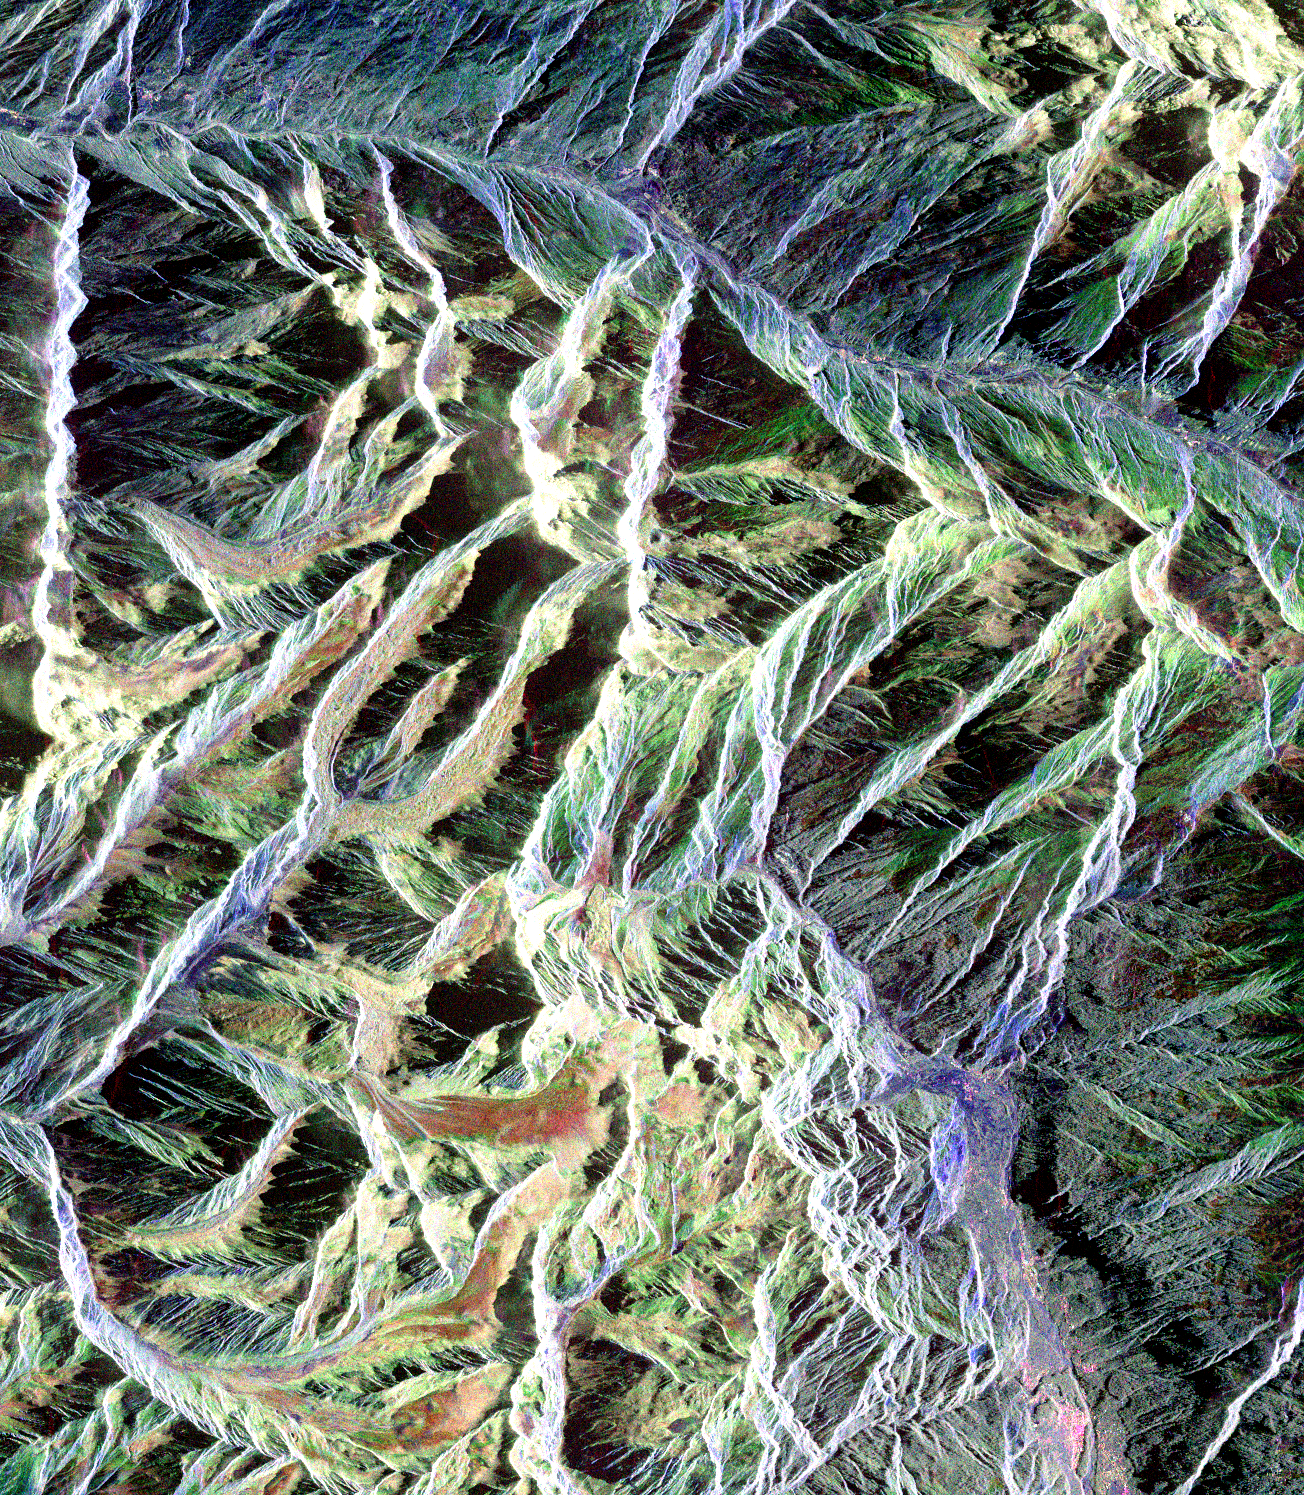
\includegraphics[width=0.6\columnwidth]{Figure_General/Manali_PauliRGB.png} 
	\caption{RADARSAT-2 Pauli RGB image of Manali-Dhundhi region,Himachal Pradesh, India}
	\label{fig:Pauli_RGB_Chennai}
\end{figure}

Furthermore, ICTD can be subdivided into eigenvalue-eigenvector-based and model-based decomposition techniques. Eigenvalue eigenvector-based decompositions provide a unique solution in terms of the scattering mechanisms~\citep{Cloude96,TOUZI2007}. These decompositions include the Von Neumann entropy ($\mbox{H}$)~\citep{john1955mathematical,cloude1986group}, the anisotropy ($\mbox{A}$)~\citep{CLOUDE97}, and the eigenvector parameters $\alpha$ and $\beta$~\citep{Cloude96,CLOUDE97}, which are assigned a physical interpretation with reference to target scattering mechanisms~\citep{cloude1986group,van1992bayesian,CLOUDE97,Cloude96}. Cloude and Pottier’s parameters have become the standard tools for target characterization and have been used as the basis for the development of new classification methods introduced for the analysis of fully polarimetric SAR data~\citep{lee1999polarimetric,pottier2000unsupervised,ferro2001unsupervised}. However,~\citep{alvarez2011coherence} raised questions regarding the assignment of each eigenvector to one of the independent scattering mechanisms by the spectral decomposition of the coherency matrix. Nonetheless, the solutions provided by model-based decompositions depend on the assumptions made about the physical scattering model. Model-based decompositions have gained considerable attention after the initial work of~\citep{freeman98}. Their decomposition assumes the target to be reflection-symmetric, i.e., the co-polarized and the cross-polarized components are always uncorrelated. This assumption was later relaxed in~\citep{Yamaguchi2005}, which included the helical scattering as a fourth component. These two decompositions are widely used in both practice and literature because of their simplicity and computational ease. Besides these, the decomposition of~\citep{arii2010general,arii2011adaptive} and~\citep{neumann2010estimation} introduced different scattering models for vegetation volume component. In~\citep{jagdhuber2013soil} this full-polarimetric decomposition with multi-angular data acquisition to estimate soil moisture from bare ground and vegetated soils have been proposed.In~\citep{cui2014complete} this a complete and an exact decomposition of the coherency matrix into a volume and two single scattering with non-negative scattering powers have been proposed. In~\citep{lee2014generalized} this the shortcomings of model-based decompositions are investigated, and suggested several models to alleviate them. Recently,~\citep{jagdhuber2014iterative} developed a hybrid model-based and eigenvalue-eigenvector based polarimetric decomposition technique with generalized volume model for soil moisture estimation under vegetation cover. 

A major advancement was made with the orientation compensation application in model-based decompositions. This was necessary because of the fact that a target with different orientations in the plane orthogonal to the radar line of sight (LOS) will have different polarimetric responses. A number of decomposition methods with orientation compensation have been proposed in~\citep{arii2011adaptive,YAMAGUCHI2011,singh13,Lee2011,An10,Chen14}. The fundamental idea behind such compensation is to minimize the cross-polarization component. The orientation compensation can, to a certain extent, reduce the overestimation of the volume power in a model-based decomposition and increase the double-bounce power. Most notably among these methods are reported in~\citep{Lee2011}, the three-component model-based decomposition by~\citep{An10}, the orientation-compensated four-component decomposition by~\citep{YAMAGUCHI2011}, and the generalized four-component decomposition by real and complex rotation of the coherency matrix by~\citep{singh13}. Most recently~\citep{bhattacharya2015adaptive} used the degree of polarization as a criteria to choose the second unitary transformation for the decomposition. The scattering powers obtained by~\cite{Yamaguchi2005} have been modified using with the concept of statistical information theory for matrices~\citep{bhattacharya2015modifying}.

\section{Factors influencing the SAR signal}
In SAR imaging, microwave portion of the EM wave signals are transmitted towards the Earth surface by an antenna. The backscattered microwave energy to the SAR system is recorded and which makes use of the conventional radar principle to form an image by utilizing the time delay. The transmitted microwave signal is scattered in all directions and the energy backscattered towards the radar is referred as radar cross-section ($\sigma$), and is a function of the amount of transmitted power absorbed and reflected by the target. The radar backscatter coefficient ($\sigma$$^\circ$) is defined as the amount of radar cross-section per unit area on the ground~\citep{jensen2000remote}. The $\sigma$$^\circ$ is a function of the wavelength, polarization, and incidence angle, as well as the target characteristics such as surface roughness, geometry and dielectric properties.

It is understood that the backscattering signal from a seasonal natural snow cover is affected by three sets of parameters: (1) snowpack parameters including snow density, free liquid water content (snow wetness), particle size and variation, characteristics of particle spatial distribution, and stratification; (2) subsurface parameters that include the dielectric and roughness properties at the snow-ground interface and (3) sensor parameters, which include the frequency, incidence geometry, and polarization;~(\cite{shi1992radar}). 

\subsection{Microwave scattering of snowpack}
The backscattering signal received by a SAR system from the snowpack is that the total sum of the surface scattering at air/snow interface, the volume scattering within the snowpack, scattering at the snow/ground interface and volume scattering from the underlying soil surface. The snow surface and volume scattering components are function of the polarization amplitude and the transmissivity respectively. Both the polarization amplitude and transmissivity depends on the dielectric constant of the medium and local incident angle. The dielectric constant of snow is primarily a function of frequency, snow wetness, temperature and density~\citep{ulaby1986microwave,hallikainen1986dielectric}. 

In case of dry snow, volume scattering is governed by dielectric discontinuities which are created by the differences in electric properties of ice crystal and air. The volume scattering increases with snow grain size and inter layering and with an increase in the amount of snow. Age of snow may influence the SAR backscatter because older snow has larger grain size than new snow grains.
The situation is totally different in the case of wet snow~\citep{ulaby1980active,stiles1980dielectric,matzler1984snow}. As soon as the top layer becomes wet (4$\%$-5$\%$ wetness by volume), the penetration capability of radar signal is reduced ~\citep{matzler1984snow}. It has been also reported in~\citep{matzler1984snow} that co-polarization ($\mbox{HH}$ and$\mbox{VV}$) backscattering coefficients of wet snow at look angle 40$^\circ$ is 10 times lower than the backscattering coefficient from dry snow and at the same time the cross polarized backscattering coefficients ($\mbox{HV}$ and $\mbox{VH}$) are 100 times lower. 

The relationship between scattering mechanism and snow wetness has been discussed in ~\citep{Shi93}. The volume scattering is inversely correlated to snow wetness. The liquid water content mainly causes an increase in snow dielectric constant which results in a significant decrease in transmission at the air/snow interface and  high dielectric loss increases the absorption coefficient. On the other hand, the surface scattering is proportional to wetness~\citep{shi1995sir}. The wavelength shift of the radar signal in snowpack was reported in~\citep{shi2000depth}. Hence, the complexity of relationship between the backscattering and snow parameters (i.e. wetness and density) makes it unrealistic to develop an empirical relationship between SAR backscattering and field measurements~\citep{singh2007envisat}. Therefore, there is need to develop inversion algorithm for snowpack parameters estimation for resolving this problem. 
  
\subsection{Influence of surface parameters} 
\begin{description}
	\item[(a) Dielectric properties:] The electrical characteristics of terrain features interact with their geometric characteristics to determine the intensity of radar returns. One measure of an object’s electrical character is the complex dielectric constant, which is a parameter that indicates the reflectivity and conductivity of various materials. The complex dielectric constant describes the ability of materials to absorb, reflect and transmit microwave energy~\citep{Campbell2002A}. Moisture content changes the electrical properties of a material, which in turn affects how the material will appear on a radar image. In~\citep{bernier1998potential} has been observed that gradual thawing of the soil caused the soil moisture and the soil dielectric constant to increase  with a resulting observed increase of backscattering signal of the snow cover. In the microwave region of the spectrum, most natural materials have a dielectric constant in the range of 3 to 8 when dry, whereas water has a dielectric constant of approximately 80. This means that the presence of moisture in soil will result in significantly greater reflectivity~\citep{ulaby1986microwave}.
\end{description}
\begin{description}
	\item[(b) Surface roughness:] The use of SAR data to retrieve surface roughness is of considerable importance in many domains, including agriculture, hydrology, and meteorology. Experimental results and studies using simulation models have shown that the radar signal is more sensitive to surface roughness at high incident angles than at low incident angles. In~\citep{holah2005potential,baghdadi2002potential,fung1994microwave,ulaby1986microwave} it has been reported that HH polarization is slightly more sensitive than VV polarization to soil surface roughness~\citep{holah2005potential}. Rough surfaces produce returns of relatively strong intensity for a wide range of depression angles~\citep{li1983tradeoffs}.
\end{description}

\subsection{Effects of SAR system parameters}  
Wavelength, polarization, incident angle and look direction are some of the important SAR system parameters. The importance of these parameters for the snowpack charaterization is presented here with more details.
\begin{description}
	\item[(a) Wavelength:] Wavelength is defined as the mean distance between two successive peak, valley or zero-crossing of a sinusoidal wave pattern and is normally measured in micrometers ($\mu\mbox{m}$) or nanometers $(\mbox{nm})$~\citep{Jensen2005introductory}. Wavelength is inversely proportional to frequency, however, When EM signal passes from one medium to another, speed of light and wavelength changes while the frequency remains the same. This wavelength interval in EM spectrum is commonly referred to as a band, channel, or region~\citep{Jensen2005introductory}. Imaging radars normally operate within a small range of wavelengths with rather broad interval. The subdivisions of the microwave region is commonly defined by $\mbox{K}_a$, $\mbox{K}$, $\mbox{K}_u$, $\mbox{X}$, $\mbox{C}$, $\mbox{S}$, $\mbox{L}$, and $\mbox{P}$ bands in ascending order of wavelength. The wavelength and the frequency range of the each band is shown in Table~\ref{table:Microwave_bands}. 	
	\begin{table}[!h]
		\caption{Microwave wavelength and frequency bands}
		\begin{tabu} to 1\textwidth { X[C] X[C] X[C]}
			\toprule
			Band & Wavelength (cm) & Frequency (GHz) \\ 
			\bottomrule
			$\mbox{K}_a$ & 0.75--1.18 & 40.0--26.5 \\ 
			$\mbox{K}$  & 1.19--1.67 & 26.5--18.0 \\
			$\mbox{K}_u$ & 1.67--2.4  & 18.0--12.5\\
			$\mbox{X}$ & 2.4--3.8   & 12.5--8.0 \\
			$\mbox{C}$  & 3.9--7.5   & 8.0--4.00 \\
			$\mbox{S}$   & 7.5--15.0  & 4.0--2.0 \\
			$\mbox{L}$  & 15.0--30.0 & 2.0--1.0\\
			$\mbox{P}$  & 30.0--100.0& 1.0-0.3\\
			\bottomrule 
		\end{tabu}
		\label{table:Microwave_bands}
	\end{table}	
	
	Radar wavelength has a fundamental influence on the interaction between the EM wave and the natural medium~\citep{garestier2006polinsar}. In principle, radar signals are capable to penetrate through the snowpack based on its wavelength and water content presents in the snowpack. In the absence of water content, penetration depth increases with the increase of wavelength~\citep{singh2009snow}. This means that longer wavelengths result in higher penetration~\citep{Campbell2002A} and could be used for mapping of wet snow~\citep{rott1993snow,nagler1996methods,shi1994snow,rao2006envisat}. The longer wavelengths are not generally useful for detecting and mapping of dry snow because snow particles are much smaller than the wavelength. It also difficult in distinguishing dry snow from bare ground using longer wavelengths SAR data. Thus, at these longer wavelengths, there is little chance for a microwave signal to be attenuated and scattered by the relatively small ice crystals comprising a snowpack~\citep{watte1970snowfield,ulaby1980active,ulaby1981microwave}. 
	
	In recent studies, it was found that the X-band image can discriminate fresh snow area from that of snow free or bare surfaces, but at C-band and L-band wavelength the signal returns may be quite similar, causing confusion in discriminating these categories. The preference of the X-band imagery with fixed channel over the C- band and L-band for general interpretation is a result of the greater sensitivity of the shorter wavelength to snow discrimination~\citep{venkataraman2008snow}. Wavelengths longer than 10–15~cm are not impeded as they move through most dry seasonal snowpacks~\citep{bernier1987microwave,bernier1998potential}. Volume scattering from a shallow, dry snow cover (SWE $<$20~cm) is undetectable at C-band (5.3~GHz, 5.6~cm), because the backscatter is dominated by soil/snow scattering. Volume scattering in dry snow results from scattering at dielectric discontinuities created by the differences in electrical properties of ice crystals and air, and by ice lenses and layers. 
		
	Atmospheric scattering is usually very small at intermediate and lower microwave frequencies and can be neglected~\citep{ulaby1980active,leconte1990preliminary,leconte1996exploring}. In case of wet snow~\citep{stiles1980dielectric,ulaby1980active,ulaby1986microwave}, when at least one layer of the snowpack (within the penetration depth of the radar signal) becomes wet (4–5~$\%$ liquid water content), the penetration depth of the radar signal is reduced to about 3–4~cm (or one wavelength at X-band)~\citep{matzler1984snow}. Thus, there may be high contrast between snow-free ground and ground covered with wet snow, thus making it possible to distinguish wet and dry snow when imaged with C-band SAR from space. Volume scattering increases with snow-grain size and internal layering, and with thickness of snow. Surface roughness is a relative concept dependent on incident microwave wavelength. 
	
	As wavelength increases, surface roughness criteria will also change. In general, more surface features will appear smoother at longer wavelengths than at shorter wavelengths. Therefore, a SAR image will appear darker in longer wavelengths than in shorter wavelengths provided the other parameters are the same~\citep{xia1997understanding}. Theoretically, azimuth resolution~(\ref{eq:azimuth_resolution_SAR}) and range resolution~(\ref{eq:range_ground_resolution_SAR}) of the SAR image is not depend on the wavelength. Therefore, wavelength will not affect the azimuth or range resolution of a SAR image. Earlier, all radar systems acquired images in a single polarization mode. Thus, relatively few studies have been carried out to examine the effect of wavelength on the detectability of snow. 
	\end{description}

\begin{description}
	\item[(b) Incidence angle:]The incidence angle is defined as the angle between the incident radar beam and the normal or vertical direction to the Earth’s surface at the point of incidence~\citep{lillesand2014remote} as shown in Figure~\ref{fig:SAR_geometry}. The look angle is defined as the angle between the vertical direction and the radar beam at the radar platform~\citep{van2011synthetic}. Depression angle is the angle between an imaginary horizontal plane and a radar beam at radar platform. Incident angle and depression angle are complementary angles, so their sum is 90$^\circ$~\citep{campbell2002introduction}. 	
		
	Radar incident angle can influence the geographical feature identification and classification to a certain degree. For low incident angle, the layover will distort the quality of SAR image in hilly terrain. For high incident angle, the radar layover is lower, but the shadow is too much, and it will lose some useful information~\citep{li2005multi}. Incident angle affects the detectability of target through its control of range resolution. On one hand, small incident angles produce poor range resolution than larger angles, as range resolution is inversely proportional to the incident angle~\citep{campbell2002introduction}. On the other hand, small incident angles provide higher spatial resolution in across track direction, improved imaging geometry in hilly and mountainous terrain (reduced foreshortening, less layover), improved thematic information content of the backscattering coefficient, and improved discrimination of small complex land cover surfaces~\citep{wegmuller2003envisat}. Experimental studies using simulation models have shown that the radar signal is more sensitive to surface roughness at high incident angles than at low incident angles~\citep{baghdadi2002potential,fung2010microwave,ulaby1986microwave,holah2005potential}.
	
	%Backscattering coefficient derived from ERS-1 data for glacier, firn and accumulation area decreases significantly at incident angle lower than 35$^\circ$ and remains almost constant between incident angle range 35$^\circ$ and 60$^\circ$. For area with vegetation and for rocks, backscattering coefficient decreases approximately linearly as incident angle increases~\citep{nagler1996methods}. For Otztal site in Alps, using ERS-1 data with low incident angle (23$^\circ$) the layover and shadow area was found 36$\%$ and 42$\%$ in ascending and descending image respectively. However, the layover area in ASAR image with swath IS6 over part of Himalayan snow cover region was found 14$\%$. The layover and foreshortening areas are more for ENVISAT swath-2 mode data which is acquired at 23$^\circ$ incidence angle. For reducing these effects, radar data at higher incidence angles (ENVISAT swath-6 or 7) are to be acquired for snow studies~\citep{singh2007envisat}.
\end{description}
	

\begin{description}
	\item[(c) Look direction: ]The direction at which the radar signal strikes the landscape, is important in both natural and man-made landscapes. In natural landscapes, look direction is especially important when terrain features display a preferential alignment. Look directions perpendicular to topographic alignment will tend to maximize radar shadow, whereas look directions parallel to topographic orientation will tend to minimize radar shadow. The extent of radar shadow depends not only upon local relief, but also upon orientations of features relative to flight path; features positioned in the near-range portion (other factors being equal) will have the smallest shadows, whereas those at the far-range edge of the image will cast larger shadows~\citep{campbell2002introduction}. Therefore it is clear that there exists a close relationship between the look direction or radar azimuth and the orientation of the topographic feature. The same type of land-cover may appear very different on a radar image due solely to a different orientation relative to the radar look direction~\citep{bryan1979effect,grey2003mapping}.
\end{description}

\begin{description}
	\item[(d) Polarization: ]Polarization is a property of certain types of waves that describes the orientation of their oscillations. The discovery of the phenomena of polarized electromagnetic energy dates back to AD 1000 when the Viking used crystals to observe the polarization of sky light under foggy condition and were able to navigate in absence of sunlight. In 1669, the first known quantitative work on light observation was published by Erasmus Bartolinus. He was followed by C. Huygens who contributed most significantly to the field of optics by proposing the wave nature of the light and discovering polarized light~\citep{lee2009polarimetric}. E.L Malus proved Newton’s conjecture that polarization is an intrinsic property of light~\citep{konnen1985polarized}. Light is a transverse electromagnetic wave. The electric and magnetic fields vibrate at right angles to the direction of propagation.  If all of the waves in a beam of light have their electric fields vibrating in the same direction, the light is described as polarized. That is, the polarization of a light wave describes the orientation of its electric field in space. Plane-polarized light has an electric field that oscillates in a specific plane perpendicular to the direction of propagation. Unlike randomly polarized light, the direction of the electric field vibration remains constant for plane-polarized light. 
	
	There are two commonly mentioned special cases of polarization, horizontal polarization, where the electric field vibrates horizontally as the wave moves forward and vertical polarization, where the electric field vibrates vertically as the wave moves forward. Plane polarized light is also called linearly-polarized light because the electric field vector can be pictured as vibrating along a line in space. If the magnitude of the electric field vector remains constant throughout each cycle, but its direction is continuously changing, the electric field can be thought of as spiraling around an axis as the wave moves forward, like the threads of an advancing screw. Elliptical polarization is the most general type of polarization. In fact, in the mathematical treatment of polarization, linear polarization and circular polarization are simply the two extremes of the elliptical case. As with circular polarization, the electric field vector rotates, but in this case the magnitude does not remain constant. That is, the tip of the electric field vector sweeps out an ellipse rather than a circle as the wave propagates.
	
	The reflected or scattered polarization characteristics of EM energy recorded by a remote sensing system can be used in many Earth resource investigations~\citep{Jensen2005introductory}. It is possible to use polarizing filters on passive remote sensing systems (e.g., aerial cameras) to record polarized light at various angles. It is also possible to selectively transmit and receive polarized energy using active remote sensing systems such as radar(e.g., horizontal transmit, vertical receive- HV; vertical transmit, horizontal receive-VH; vertical transmit, vertical receive-VV; horizontal transmit, horizontal receive-HH).
	
	Multi-polarized information about the target or Earth surface recorded by the radar system is a special interest for the bio-\ geo-physical parameter investigations. In~\citep{shi1995sir}, found that the surface and volume interaction terms are the important scattering source for cross polarized signals. The surface-volume interaction terms under the independent assumption result in an over-estimation for HH polarization. For VV polarization, however, it always over-estimates at small incident angle and under-estimates at large incidence angle. The importance of multi-frequency and multi-polarization data for separating different snow and ice regimes on glaciers and for mapping accumulation and ablation areas has been analyzed by~\citep{rott1995snow}. L- or C-band co- and cross-polarized channels in combination with X-band were found to be of main importance for snow and glacier applications. Multi-polarized, multi-frequency microwave data can suffice the needs up to some extent when a simplified form of Integral Equation Method (IEM) is used. 
	
	The single band (C-band) SAR data is inadequate for the estimation of snow wetness because which takes more than one unknown parameter into consideration. The effect of the snow volume scattering albedo and surface roughness can be minimized to estimate the snow parameters using multi-polarization(dual polarization) backscattering coefficient (HH, VV and Re{[\mbox{HHVV}]}) measurement~\citep{Shi95wetness}. In~\citep{autret1989theoretical} and ~\citep{chen1995simple} also have reported that the influence of surface roughness can be minimized using the co-polarized ratio (HH/VV). Hence, multiple polarizations helps to distinguish the physical structure of the scattering surfaces. Co-polarization signals are dominated component for surface scattering eg., $\mbox{VV}$ polarization and cross-polarization is the dominant component for volume scattering eg.,$\mbox{VH}$ polarization.
	
	By comparing both the $\mbox{HH}$ and $\mbox{HV}$ images, the features and areas that represent regions on the landscape that tend to depolarize the signal can be identified. Such areas will reflect the incident horizontally polarized signal back to antenna as vertically polarized energy- that is they change the polarization of the incident microwave energy. Such areas can be identified as bright regions on the $\mbox{HV}$ image and as dark or dark grey regions on the corresponding HH image. The polarization of the energy that would have contributed to the brightness of the $\mbox{HH}$ image has been changed, so it creates instead a bright area on the HV image. The same information can be restated in a different way. A surface that is an ineffective depolarizer will tend to scatter energy in the same polarization in which it was transmitted; such areas will appear bright in the HH image and dark on the HV image ~\citep{campbell2002introduction}. The alternating polarization mode of ASAR is capable of providing multi-polarimetric acquisitions by means of SAR acquisitions, where switching is made on polarizations instead of sub swaths. Each of these polarizing channels have varying sensitivities to different surface characteristics and properties. For example, the dynamic range of the like polarized component is larger than that of the cross-polarized component for snow cover area~\citep{shi1997estimation}; this is in contrast to the measurement for forested areas, where the dynamic range of the cross-polarized component is larger than that of the like-polarized component~\citep{dong1997radar}. 
	
	The information from alternative polarization of SAR images are the great importance in the process of identification and classification of different types of scattering mechanisms, and where the penetration depth is different at different polarization channels. However, use of satellite SAR polarimetry data sets for snow cover area analysis is only a beginning and there are still many unknowns. Given the paucity of data analysis of snow covered area with multi-polarized data sets and the variation in the earlier results much remains to be determined about the exact relationships between snow parameters and radar backscatter. In~\citep{venkataraman2008snow}  have reported that the backscattering coefficient value of $\mbox{HH}$ polarization is lower than the $\mbox{VV}$ polarization while studying the snow wetness in the Himalayan snow covered region. 
\end{description}
\subsection{Snowpack parameters}
\label{sec:2.3}
Microwave signal interaction with targets (e.g. snow) changes mainly according to the frequency (or wavelength) and the polarization. The interaction depends on the shape and orientation of the scatters and the scattering mechanisms (i.e. whether it is single or multiple scattering). The polarization characteristics get vary for different polarization channels for the same target. By using imaging radar, the polarimetric characteristic can be measured for each pixel to understand the scattering mechanism associated with it. The geophysical information associated with the scattering mechanism could be inferred from these polarimetric responses. Generally, single frequency and single polarization radar techniques have a considerable degree of ambiguity for different types of targets. To overcome this, the dimensionality of the observation needs to be increased. This can be achieved through the use of multi-frequency and/or multi-polarization radar systems. Multi-temporal and multiple incident angles are other ways of increasing the dimensionality of observation. In this section important estimation of snowpack parameters (wetness and density) relative to the proposed objectives and their characteristics is discussed through the available literatures. Exhaustive review of mountainous snow cover properties using active microwave remote sensing is presented in~\citep{snehmani2015review}.

\begin{description}
	\item[(a) Snow wetness: ] Snow wetness is a percentage of free liquid water presented in the snowpack. This is an useful indicator for the prediction of snow melt start and runoff and also a important parameter for the prediction of avalanches, flooding, global warming, and climate change. Estimating snow wetness requires a good understanding on the scattering mechanism of wet snow. This is a very complex task due to the highly variable physical structure of wet snow. Effective permittivity of snowpack is highly depended on the presence of water droplets or particles in it. For dry snowpack, the backscatter contribution from the air-snow surface is small and thus can be neglected. So, the total backscatter contribution is a combination of snow volume and snow-ground surface only~\citep{Shi2000}. 
	
	For dry snow, the penetration depth, $\delta_p\approx$ 10~m at 10~GHz and decreases to 1~m at 40~GHz~\citep{Rott85}. Volume scattering in snow is due to dielectric discontinuities. Volume scattering from thin dry snow cover is undetectable at wavelengths longer than 10 or 15 cm, however, the level of scattering is dependent on the amount of snow on the ground (more snow implies more dielectric discontinuities for scattering)~\citep{bernier1987microwave}. The extinction coefficient, $\kappa_e$ which is inversely related to $\delta_p$ is equal to the sum of the absorption coefficient ($\kappa_{a}$) and scattering coefficient ($\kappa_{s}$). For wet snow, $\kappa_{e}\approx\kappa_{a}$, at microwave frequencies as the absorption losses are much larger than the scattering losses. Due to this, $\delta_p$ is of the order of 1 or 2 wavelengths and hence, the snow-ground scattering may be neglected. For C-band SAR, the backscattering signal from wet snow is dominated by the scattering from air-snow interface and snow volume medium~\citep{Shi95wetness}.
	SAR backscattering coefficient is sensitive to many snow parameters that hydrologist use, especially free liquid water content in the snowpack because of the large dielectric contrast between ice and water in microwave spectrum (~\citep{Shi93}. Several investigators~\citep{Arslan05,shi1992radar,shi1997estimation,Shi95wetness,strozzi1999mapping,Singh2007_spie,singh2010snow} reported that backscatter coefficient image of radar is extremely useful for the quantitative estimation of snow wetness (percentage of liquid water content in snowpack).
	 
	L band, horizontal polarization SAR shows that the backscattering coefficient ($\sigma^0$) decreases with increase in snow depth and snow wetness for a given snow density and surface roughness.  The variation in grain size does not seem to affect this relation.  In case of dry snow, there is very little change in $\sigma^0$ with change in snow depth.  Using this relation, it may be possible to derive snow wetness from backscatter coefficient if we know the snow depth.  However, it is not credible to derive a simple empirical relation between snow wetness and radar backscattering, as previous investigations have shown both negative and positive relationships between backscattering coefficients and snow wetness~\citep{Shi95wetness}. This relationship is complicated, as surface roughness affects this relationship. Surface roughness affects the relationship between the backscattering coefficients and snow wetness.  For low wetness ($\le 3\%$) the dielectric contrast between air and snow is small and volume scattering dominates, so backscattering is now sensitive to surface roughness and decreases as wetness increases.  However, for wetter snow, backscattering becomes sensitive to surface roughness, because the surface-scattering component increases while the volume-scattering component decreases. Thus the relationship between backscattering and snow wetness is controlled by the scattering mechanism.  When the surface is smooth, volume scattering is the dominant scattering source. 
	
    As snow wetness increases, both the volume scattering albedo and the transmission coefficients greatly decrease.  This results in a negative correlation between the backscattering signals and snow wetness.  When the surface is rough, increasing snow wetness results in greatly increased surface scattering interaction and surface scattering becomes the dominant scattering process.  Therefore, a positive correlation between the backscattering signals and snow wetness will be observed~\citep{Shi93}. Moreover, the relationship between co polarization and snow wetness can be either positive or negative, depending on snow characteristics, surface roughness and incidence angle. In~\citep{Singh2007_spie}, an empirical model has been developed for the estimation of snow wetness using $\mbox{HH}$ polarization backscattering coefficient. It has been observed that, the backscattering coefficient is approximately constant for the snow wetness values ranges from 3.0$\%$ - 5.0 $\%$.  This complexity of the relationship between the backscattering coefficient and snow wetness makes it unrealistic to develop a simple empirical relation. 
		
	A inversion model has been developed for the estimation of snow wetness based on Small Perturbation Model (SPM)~\citep{Shi93}. This model is applicable for the incidence angle ranges from 15$^\circ$-70$^\circ$ and for the small to moderate surface roughness variations. Further,~\citep{Shi95wetness} used fully polarimetric space shuttle borne SIR-C data to derive snow wetness by inverting a first order backscatter model (surface and volume scattering). By measuring three components ($\sigma_{vv}^0$= Backscattering Coefficient (BSC) of VV polarization, $\sigma_{hh}^0$ = BSC of HH polarization and $\sigma_{vvhh}^0$=$Re[VVHH^*]$) they were able to minimize effects from volume scattering and surface roughness (i.e. reduce the dimensionality of inversion problem) to estimate snow permittivity, which subsequently is related to snow wetness.~\citep{singh2006snow} also developed dielectric retrieval algorithm using first order surface scattering and volume scattering based on Physical Optics Model (POM). Further the dielectric constant has been related to snow wetness. Absolute error between Envisat-ASAR estimated and field measured value was observed to be 2.52$\%$ by volume.
	
	~\citep{Kendra98} conducted experiments to measure radar backscatter at C and X band of artificial snow of varying depths. The results of this study are amenable to comparison with predictions based on theoretical methods for modeling volume scattering media.  A direct polarimetric inversion approach has been described through which the characteristics of the snow medium are extracted from the measured data.~\citep{Kendra98} have also collected backscatter values alongwith concurrent snow liquid water content (wetness) measurements in experimental snowpacks. These measurements were used to confirm the validity of the algorithm developed by~\citep{Shi95wetness} for the retrieval of snow liquid water content. It has been found that the algorithm was able to precisely characterize the snowpacks for their wetness.~\citep{niang2007new} also developed statistical inversion model which performs retrieval of the snow wetness using ENVISAT- ASAR alternating polarization data.~\citep{Shi95wetness} model required fully polarimetric SAR data, but ENVISAT-ASAR has capability of data acquisition in dual polarization only. Hence,~\citep{singh2010snow} modified~\citep{Shi95wetness} snow wetness algorithm for dual polarization and the modified algorithm was implemented on ENVISAT-ASAR dual polarization data.  Model estimated wetness was found to be quite in agreement with measured wetness with 2.8$\%$ absolute error.	
\end{description}

\begin{description}
	\item[(b) Snow density: ] In general, snow is electromagnetically a three component dielectric mixture of ice, water and air. Dry snow is an inhomogeneous medium consisting of ice particles and air voids, whereas wet snow consists of ice spheres embedded in an air-water medium. Snow density is an important parameter of the snowpack which influences the thermal, mechanical and optical properties of snow layers. It is thus a vital parameter for avalanche prediction~\citep{hirashima2009adjustment,brun1989investigation} and snow hydrology~\citep{rango1995revisiting,jonas2009estimating,sturm2010estimating}. The snow density is a complex parameter that can vary spatially, temporally and vertically within the snowpack profile~\citep{bormann2013spatial}. Wind erosion, melt-refreeze events, compaction and snow metamorphisms acting in response to internal temperature and moisture gradients~\citep{sommerfeld1970classification,colbeck1982overview} are responsible for seasonal snowpack densification. The snow particles get reshaped into sphere-like structures due to wind erosion. These sphere shaped particles, then closely pack together thereby increasing the density. The melt-freeze processes~\citep{colbeck1982overview} due to temperature fluctuations is majorly responsible for snow densification. The liquid water content present in the snowpack~\citep{brun1989energy,marshall1999snow} along with the destructive snow metamorphisms occurring when vertical temperature gradients are weak~\citep{colbeck1982overview} results in smaller and rounded particles. Bulk weight density of snow according to EN 1991-1-3 and NS 3491-3 (settled snow is measured several hours or days after its fall; old snow several weeks or months after its fall). 	As given in NS 3491-3 and EN 1991-1-3 (European Committee for Standardization, 2003) the mean density of snow is given in~Table~\ref{table:mean_density_of_snow}~\citep{MET40}.
	
	\begin{table}[!htbp]
		\caption{Mean density of different snow types}
		\centering
		\begin{tabu} to 0.8\textwidth { X[l] X[r]}
			\toprule
			Type of snow & Bulk weight density (kg m $^{-3}$) \\ 
			\bottomrule
		\end{tabu}
		\begin{tabu} to 0.8\textwidth { X[l] X[r]}
			Fresh & 100 \\ 
			Settled & 200\\ 
			Old & 250-350\\
			Wet & 400 \\
			\bottomrule
		\end{tabu}
		\label{table:mean_density_of_snow}
	\end{table}
	
	Several works have been done with the microwave interaction of snow at various frequencies~\citep{stiles1980active,ulaby1980active,ulaby1984snowcover,rott1987possibilities,rott1988study}The radar backscattering coefficient is a function of various parameters classified as surface parameters and radar observation parameters. The radar observation parameters include the transmission wave frequency, polarization, and incidence angle. Surface parameters include roughness, geometrical shape and dielectric properties of the target. SAR data showed its potential for snow cover monitoring in the boreal forest zone~\citep{koskinen1997use}. Several theoretical models have been developed and experimental data sets have been analyzed to relate backscattered coefficient of snow covered terrain with its physical properties~\citep{Shi95wetness,Shi2000,shi2000depth,besic2012dry,besic2015stochastic}. All these studies have indicated that the factors which have been found to have the most profound influence on the backscatter coefficient are snow water equivalent, liquid water content and moisture content of soil. The snow surface roughness and size distribution of ice crystals are also some of the important factors and the extent of their importance is further dependent on the wavelength used and the angle of incidence. Satellite remote sensing is a key tool in monitoring the snow pack parameters over a large area. Microwave remote sensing measurements can be efficiently used to infer bulk properties of snowpack. 
	
	Many algorithms have been developed for SAR data to estimate the snow dielectric constant~\citep{Shi93,Shi95,Singh2007_spie,niang2007new,singh2010snow,surendar2013improved,bhattacharya2014snow}. The real part of the relative dielectric constant~($\varepsilon{'}$) is solely dependent on the density. An inversion approach for the estimation of snow density from full polarimetric SAR data was developed by~\citep{Shi2000} using L-band data from SIR-C/XSAR mission. This algorithm does not require a priori knowledge of the subsurface dielectric and roughness properties and it can be applied over a large range of incident angles (10$^\circ$-70$^\circ$). The estimated snow density compared to field measurements shows an RMSE of 0.042 gcm$^{-3}$ and a relative error of 13$\%$. However, this method cannot be applied where the subsurface is dominated by volume scattering, as may be the case with snow-covered firn. Even though they used full polarimetry data, they did not utilize the complete full-polarimetric information. However, they have only considered a first order backscattering coefficients to invert snow density. There are many snow and glacier studies done over the Indian Himalayan region using fully polarimetric SAR  data~\citep{singh2011a,singh2012a,singh2012b,singh2014a,singh2014b}. Dry snow density estimation algorithm over the Indian Himalayan region was proposed in~\citep{Snehmani2010density}. In this, C-band ENVISAT-ASAR data has been used and snowpack volume and snow-ground scattering components were considered for the inversion. Very recently,~\citep{surendar2015density} demonstrated and validated the snow wetness and density estimation algorithms based on full polarimetric C-band Radarsat-2 data over Indian Himalayan region. The snow density algorithm accounted for only a snowpack volume scattering for the C-band data. 
	 
\end{description}
	
\section{Current PolSAR reserch for snowpack parameter studies}
	Recently, some ad-hoc programmes initiated to study the global snow cover to understand the fresh water storage. In particular, the ESA’s Cold Regions Hydrology high-resolution Observatory (CoReH2O) mission offers many researchers to carried out the study on snow parameters estimation. Some SAR sensors onboard Unmanned Aerial Vehicle (UAV) (Ex., snowSAR) was also flown to study the snowpack characterization with high amount of accuracy. The availability of high spatial temporal resolution and multi-polarization $\&$ multi-frequency SAR systems provide an opportunity to researchers to explore more precise snowpack information. A new empirical relationship has been developed for the estimation of SWE using X-band COSMO SkyMed $\mbox{VV}$ polarization data~\citep{Pettinato2013}. This empirical relationship may be highly depends on the study area and data acquisition time and weather conditions. This method is also valid only for dry snow cover with the snow depth in the range of 60-70cm. 
	
	
	Rott et al. (2014) and Macelloni et al. (2014) used the minimization approach to estimate the SWE over the terrain and forest cover area respectively using multi-frequency dual polarization SnowSAR data. This methods need priori information to apply the minimization and retrieve SWE and this methods are applicable only for dry snow cover. Leinss et al. (2014 (a)) estimated the fresh snow depth using co-polarization phase difference of X-band SAR data.  They have presented the relationship between the microstructure of snow and the co-polarization phase difference and have also studied the variation of CPD with respect to the temperature gradient.  Leinss et al. (2014 (b)) have also presented an approach for estimation of SWE using differential interferometry technique. They have derived a linear function between the SWE and the phase difference for dry snow using Ku and X band SnowScat instrument. Very recently, Surendar et al. (2015 (a), 2015 (b)) demonstrated and validated the snow wetness and density estimation algorithms based on full polarimetric C-band Radarsat-2 data over Indian Himalayan region. The snow density algorithm accounted for only a snowpack volume scattering for the C-band data. Further this algorithm can be modified and suitably used for higher wavelength bands and for complete dry snowpack conditions. 
	
\chapter{Development of Algorithms and Methodologies}
\label{sec:3}
In this chapter, all the new algorithms developed during the course of this work for the estimation of snow parameters from polarimetric SAR systems are explained. All the new methodologies are presented with detailed flowcharts and derivations. The detailed description about the study area, in-situ field data collection and the data sets used for this study are also incorporated in this chapter.

\section{Snow wetness estimation using dual polarimetric SAR data}
\label{sec:3.1}
In this section, a new snow wetness estimation method from dual-polarimetric coherent (HH/VV) SAR data
(i.e., TerraSAR-X) is developed which is based on the work of~\cite{jagdhuber2013polarimetric} for the estimation of soil moisture. In wet snow, the surface and the volume are the dominant scattering mechanisms. The snow surface wetness is estimated by using the simplified IEM model for high frequency limit of X-band (9.6 GHz) data. The snowpack volume wetness is estimated under the Rayleigh scattering assumption. The proposed method is used to estimate the snow wetness of the top layers ($\approx$ 15~cm) of the snowpack. 

The dual-polarimetric coherent TerraSAR-X data can be represented by a $2\times2$ coherency matrix ([$T_2$]) given in~(\ref{eq:coherency_matrix_dual}). In this study, we will analyze this coherency matrix to estimate the snow surface and the snow volume wetness. 
\begin{equation}
{
\mathbf{\langle[T_2]\rangle}= \frac{1}{2} \left[ \begin{array}{ccc}
<|S_{HH}+S_{VV}|^2> & <(S_{HH}+S_{VV})(S_{HH}-S_{VV})^*>\\
<(S_{HH}+S_{VV})^*(S_{HH}-S_{VV})> & <|S_{HH}-S_{VV}|^2>\\
\end{array}\right]	
 }
\label{eq:coherency_matrix_dual}
\end{equation}
In order to estimate the snow surface wetness, the simplified IEM scattering model is used to obtain the dominant scattering magnitude $(\alpha_1)$ under the high frequency limit of X-band (9.6 GHz)~\citep{allain2003}. The IEM model has been shown to be valid for a wide range of surface roughness~\citep{Fung92,fung1994microwave}. Usually a wet snow surface is rougher than a dry snow surface because of selective melting and re-freezing.  

A snow layer is an inhomogeneous medium composed of ice particles and water inclusions of different shapes, sizes, and orientations~\citep{Shi95wetness}. At a given sensor frequency, the snow density and the liquid water content affect the permittivity of snow. The Rayleigh scattering assumption has been used for the study of snowpack volume wetness, where the particles of the medium are considered substantially smaller than the incident wavelength. Finally, the effective snow wetness is obtained by suitably weighing the surface and the volume snow wetness components. The weights are obtained from the eigen-decomposition of the [$\mbox{T}_2$] matrix.

The in-situ measurements were obtained synchronously with the TerraSAR-X pass in January. Snow wetness measurements were taken at every 5~cm depth of the standing snow. The average wetness measurement is considered as the effective snow wetness which is then used to validate the results obtained from the proposed method.

\subsection{Snow surface wetness}
The dominant polarimetric scattering angle $(\alpha_1)$, corresponding to the dominant eigenvector and the eigenvalue is obtained from the dual coherent [$T_2$] matrix as shown in~(\ref{eq:alphas}).
\begin{equation}
\begin{split}
[T_2] &= [U_2][\Sigma][U_2]^{T} \\
U_2 &= \left[ \begin{array}{ccc}
u_{11} & u_{12} \\
u_{21} & u_{22} \\
\end{array} \right] \\
\alpha_1 &= \cos ^{ - 1}(|u_{11}|) 
\end{split}
\label{eq:alphas}
\end{equation}
where $[U_2]$ is a 2$\times$2 unitary matrix of the eigenvectors, $[\Sigma]$ is a $2\times2$ diagonal matrix of the eigenvalues and the superscript $T$ denotes matrix transpose. In the high frequency limit, like X-band (9.5 GHz), the dominant polarimetric scattering angle $(\alpha_1)$ obtained from the dual-polarimetric data is compared with the scattering angle $(\alpha_{IEM})$ estimated from the simplified IEM model for high frequency $(\nu)$ limit of X-band data ~(\ref{eq:highfreq})~\citep{allain2003}. 
\begin{equation}
\alpha_1 \approx \lim\limits_{\nu \rightarrow High}(\alpha_{IEM}) 
\label{eq:highfreq}
\end{equation}
The estimated $(\alpha_{IEM})$ from the simplified IEM model is only a function of the local incidence angle ($\theta$) and the surface dielectric constant $(\varepsilon_s)$ and is independent of the terrain roughness~(\ref{eq:iemalpha}). The local incidence angle $(\theta)$ is obtained using an external DEM (e.g. SRTM DEM).
\begin{equation}
\begin{split}
\lim\limits_{\nu \rightarrow High} (\alpha_{IEM}) &= \atan\left( \frac{2f_{hh}f_{vv}^{*}-X}{2f_{hh}f_{vv}^{*}+X}\right) \\
X = \left|f_{vv}\right|^2 - \left|f_{hh}\right|^2 + &\sqrt{\left(\left|f_{vv}\right|^2 - \left|f_{hh}\right|^2\right)^2 + 4\left|f_{hh}f_{vv}^{*}\right|^2}
\end{split}
\label{eq:iemalpha}
\end{equation}
The $f_{hh}=-\frac{2F_{hh}}{\cos\theta}$ and $f_{vv}=\frac{2F_{vv}}{\cos\theta}$ are the co-polarization scattering coefficients, where $F_{hh}$ and $F_{vv}$ are the Fresnel reflection coefficient for each polarization as a function of the local incidence angle $(\theta)$ and the dielectric constant $(\varepsilon_s)$. This estimated surface dielectric constant $(\varepsilon_s)$ is then used to compute the snow surface wetness using the Denoth's method $(W_s (\rho_d,\varepsilon_s))~\eqref{eq:denoth}~$~\citep{denoth1995electron}, where $\rho_d$ is the dry snow density.

\subsection{Snow volume wetness}
Apart from the snow surface wetness component, a small amount of snow volume wetness component is also expected with X-band data from a standing snow cover over ground since the penetration depth of the probing wave will be limited. The volume scattering of the snowpack is modeled as a random volume in this study. The snowpack particle structure shows high spatial variation and as a result of which it is difficult to model its volume scattering component. In this context, the particle anisotropy has been used to account for all snow particle structures. The anisotropy parameter which is interpreted in terms of the particle geometry is also characterized by the ratio of principal values of polarizability~\citep{cloude2009polarisation}. A random volume scattering coherency matrix is used in this study~(\ref{eq:volumemodel}) where $f_v$ is the volume scattering intensity and $A$ represents the particle anisotropy. 
\begin{equation}
\begin{split}
\frac{f_v}{(1+A^2)} \left[ \begin{array}{cc}
V_{11} & V_{12} \\
V_{12}^* & V_{22} \\
\end{array} \right]= \left[ \begin{array}{cc}
\frac{1}{2} & 0 \\
0 & \frac{1}{4} \\ 
\end{array} \right] \\
V_{11} = \frac{1}{2} (A+1)^2 ; V_{12} = 0 ;
V_{22} =\frac{1}{4}(A-1)^2 \\
\end{split}
\label{eq:volumemodel}
\end{equation}

The volume scattering intensity ($f_v$) is a function of the cross-polarization component ($S_{xx}$) in quad-polarimetric case. But, unlike in the quad-polarimetric data, the cross-polarization component is unavailable in the dual-polarimetric X-band $(\mbox{HH/VV})$ coherent data. Hence, this cross-polarization component is synthesized from the dual-polarimetric data under the azimuthally symmetric condition~(\ref{eq:crosspolestimation}).  
\begin{equation}
\begin{split}
f_v &= 8<|S_{xx}|^2> \\
<|S_{xx}|^2> &= \frac{1}{4} \left(1-\gamma_{HHVV}\right)\left(<|S_{HH}|^2>+<|S_{VV}|^2>\right) \\
\gamma_{HHVV} &= \frac{<S_{HH}S^*_{VV}>}{\sqrt{<|S_{HH}|^2><|S_{VV}|^2>}}
\end{split}
\label{eq:crosspolestimation}
\end{equation}
The quality of the estimated cross-polarization component cannot be assessed in this study due to the unavailability of a quad-polarimetric TerraSAR-X data along with the dual-polarimetric (HH/VV) coherent data. However, it has been shown that the Root Mean Square Error (RMSE) of the synthesized cross-polarization component for the TerraSAR-X data is around 1.8-2.0 dB compared to 5.0-5.4 dB for L-band E-SAR data over agricultural areas~\citep{Jagdhuber2014}. In this work our study area is a snow cover over flat bare ground devoid of any vegetation for which the condition of azimuthal symmetry can be assumed to be valid. By solving for the particle anisotropy $(A)$, it can be readily seen that it is a function of the volume scattering intensity $(f_v)$. In general the anisotropy parameter which is an indicator of particle shape is also bounded by the dielectric constant~(\ref{eq:anisotropy})~\citep{ablitt2000characterisation}. This dielectric constant is then used to estimate the volume snow wetness.
\begin{equation}
\frac{1}{\varepsilon_v} < A < \frac{\varepsilon_v + 1}{2}
\label{eq:anisotropy}
\end{equation}

In order to have an approximate estimate of $\varepsilon_v$, we have combined the lower and the upper bounds of the inequality involving the anisotropy parameter and $\varepsilon_v$. Any estimate of  $\varepsilon_v$ cannot lie below the curve given by $1/ A$ and below the line given by $2A-1$. An estimating function for $\varepsilon_v$ satisfying both these conditions is given by~(\ref{eq:volumedielctric}). As the value of the anisotropy parameter increases from 0 to 1, there is a rapid fall in the estimate of $\varepsilon_v$ as dictated by the lower bound. At $A=1$, the lower and the upper bounds of the inequality converge, and $\varepsilon_v$ is estimated as unity. Beyond this point there is a linear rise in the estimate of $\varepsilon_v$. 
\begin{equation}
\varepsilon_v = \frac{1}{A} + \left| \frac{1}{A} - (2A - 1)\right|
\label{eq:volumedielctric}
\end{equation}
\begin{equation}
W_e=
\begin{cases}
\bar{\lambda}_{1}W_s(\rho_d,\varepsilon_s) + \bar{\lambda}_{2}W_v(\rho_d,\varepsilon_v) \quad: W_s(\rho_d,\varepsilon_s) > W_v(\rho_d,\varepsilon_v) \\ 
\bar{\lambda}_{1}W_v(\rho_d,\varepsilon_v) + \bar{\lambda}_{2}W_s(\rho_d,\varepsilon_s) \quad: W_v(\rho_d,\varepsilon_v) > W_s(\rho_d,\varepsilon_s) \\
\end{cases}
\bar{\lambda}_{i} = \frac{\lambda_i}{\sum_{i=1,2}^{}\lambda_i}, \quad
\bar{\lambda}_{1} > \bar{\lambda}_{2}
\label{eq:effectivewetness}
\end{equation}
Similar to the snow surface wetness estimation, the volume dielectric constant $\varepsilon_v$ is used to estimate the snow volume wetness using the Denoth's method $(W_v (\rho_d,\varepsilon_v))$~\eqref{eq:denoth}, where $\rho_d$ is the dry snow density as used before. The effective snow wetness $(W_e)$ is estimated as a weighted average of the surface and the volume snow wetness according to~(\ref{eq:effectivewetness}). The pseudo probabilities computed from the eigenvalues are used to weigh $W_s(\rho_d,\varepsilon_s)$ and $W_v(\rho_d,\varepsilon_v)$ to estimate $W_e$. In the high frequency limit for the wet snow cover condition ($W_s(\rho_p,\varepsilon_s) > W_v(\rho_d,\varepsilon_v)$), the surface scattering is mostly the dominant scattering mechanism. Owing to this criteria, the surface wetness $W_s(\rho_d,\varepsilon_s)$ is weighted with the first dominant eigenvalue, $\bar{\lambda}_{1}$ and subsequently the volume wetness $W_v(\rho_d,\varepsilon_v)$ is weighted with the second dominant eigenvalue, $\bar{\lambda}_{2}$. In some cases (fairly less), when $W_v(\rho_d,\varepsilon_v) > W_s(\rho_d,\varepsilon_s)$, the volume wetness, $W_v(\rho_d,\varepsilon_v)$ is weighted with the first dominant eigenvalue, $\bar{\lambda}_{1}$ and the surface snow wetness, $W_s(\rho_d,\varepsilon_s)$ is weighted with the second dominant eigenvalue, $\bar{\lambda}_{2}$ to calculate the effective snow wetness $W_{e}$. The flowchart of the proposed snow wetness estimation methodology is shown in Figure~\ref{fig:flow_chart_sw_dual_pol}.
\begin{sidewaysfigure}[!htbp]
		\centering
		\includegraphics[width=0.6\columnwidth]{Figures_SW2/flow_chart}
		\caption [Flowchart of snow wetness estimation method for dual-pol data]{Flowchart of the proposed snow wetness estimation methodology.}
		\label{fig:flow_chart_sw_dual_pol}
\end{sidewaysfigure}	
\section{Snow wetness estimation using full polarimetric SAR data}
\label{sec:3.2}
In this section, a novel inversion model for the estimation of snow wetness from full-polarimetric SAR data is explained. This inversion technique is based on the G4U scattering power polarimetric decomposition technique. In wet snow, the surface and the volume are the dominant scattering mechanisms, therefore the generalized surface and the volume parameters are adopted. These parameters are then directly used to estimate the surface and the volume snow wetness. The effective snow wetness map is derived from the weighted average of both the wetness maps. The weights are derived from the normalized surface and volume scattering powers. 
\subsection*{Introduction}
The radar backscattering coefficient has been very useful for the quantitative estimation of snowpack parameters. Ground-based experiments were conducted to study the effect of dry and wet snow to backscattering coefficient of terrain~\citep{Stiles1980}. The measured backscattering coefficient is a function of several snow and soil parameters: snow layer, thickness, snow temperature, snow wetness, snow density, surface roughness (air-snow interface as well as snow-ground interface)~\citep{ulaby1986microwave}. Radar backscattering effects on geographical areas, relief, aspect angle, layover and shadow have also been studied~\citep{Koskinen97,Nagler2000,small2011flattening}. The snow volume scattering has been modeled by a discrete particle model which was experimentally justified at C-band~\citep{Kendra98,Koskinen2000}. A semi-empirical model for radar backscattering coefficient of snow covered ground was developed at 35~GHz and 95~GHz frequencies~\citep{Ulaby95}. This model relates the backscatter coefficient to the incidence angle and the snow-pack parameters (snow depth, crystal size and liquid water content) for each linear polarization.  

Several models have been developed to predict backscattering from rough surfaces: (1). the physical optics model, (2). the geometric optics model, (3). the small perturbation models (SPMs) and (4) the integral equation model (IEM) which is valid for a wide range of surfaces~\citep{Fung92,fung1994microwave}. Possibly due to surface roughness, several studies have shown both positive and negative correlation between the backscatter coefficient and snow wetness~\citep{stiles1980dielectric,shi1992radar}. Several algorithms for snow covered area retrieval have observed a negative correlation between the backscatter coefficient and wetness values for reasonable snow wetness and depth~\citep{Koskinen97,Nagler2000,Guneriussen2001b}. A inversion model has been developed to estimate snow wetness based on the first-order scattering model considering both surface and volume scattering~\citep{Shi93}. The NASA/JPL airborne AIRSAR imaging polarimetric data was used in this study. However, the first-order scattering model does not fit to most natural surfaces as they are very rough on the radar wavelength scale. The Integral Equation Model (IEM) which is valid over a wider range of surface roughness is used for the inversion model to estimate snow wetness~\citep{Shi95wetness}. The polarimetric space-borne Shuttle Imaging Radar Mission C-band (SIR-C) data was used for this study. The above method was modified to estimate snow wetness from conventional dual-polarization ENVISAT-ASAR data~\citep{singh2010snow}. A statistical inversion model was also developed to retrieve snow wetness using ENVISAT-ASAR alternating polarization data~\citep{niang2007new}. Recently, a new snow wetness estimation methodology has been proposed which utilizes the full-polarimetric SAR decomposition technique~\citep{Surendar13a}. 

A major advancement was made with the orientation compensation application in model-based polarimetric decompositions. This was necessary because of the fact that a target with different orientations in the plane orthogonal to the radar line of sight (LOS) will have different polarimetric responses. A number of decomposition methods with orientation compensation have been proposed to alleviate this issue~\citep{Lee2011,An10,YAMAGUCHI2011,singh13,arii2011adaptive,Chen14}. In the context of this work, the orientation compensation on the coherency matrix is important because of the gentle to very steep slopes of the Himalayan topography. These slopes vary in azimuth as well as in the range direction due to which there is an appreciable distortion in the backscattering observed in the Himalayan region as compared to horizontal flat surfaces. The polarization orientation shift or equivalently the cross-~polarization component is induced due to the azimuthally sloped surfaces~\citep{Lee2000,Lee2002}. In addition, the amount of the induced polarization orientation shifts is also a function of the radar look angle and the slope angle in the range direction. These effects in highly topographically irregular surfaces can be reduced with the help of polarization orientation compensation or minimization of the cross-polarized component. 

The Yamaguchi four-component decomposition with rotation of the coherency matrix (Y4R)~\citep{YAMAGUCHI2011} is the most frequently used method in SAR polarimetry. The Himalayan topography with gentle to steep slope behave like oriented surface from the radar illumination direction which causes the overestimation of the volume scattering component in the original Yamaguchi decomposition method (Y4O)~\citep{Yamaguchi2005}. The modified method (Y4R) compensates for the orientation changes along the radar line of sight which consequently decreases the volume scattering power. In this work we have used the general four-component scattering power decomposition method (G4U)~\citep{singh13} which is implemented by a double unitary transformation of the coherency matrix~(\ref{eq:g4u_decomposition_1} and~\ref{eq:g4u_decomposition_2}), 

\begin{subequations}
	\begin{multline}
	\left\langle\mathbf{[T(\theta)]}\right\rangle = \left[U(\theta)\right]\Bigl(f_{s}\left\langle\mathbf{[T]}\right\rangle_{surface} +  f_{d}\left\langle\mathbf{[T]}\right\rangle_{double} + f_v\left\langle\mathbf{[T]}\right\rangle_{vol} \\ + f_{c}\left\langle\mathbf{[T]}\right\rangle_{helix}\Bigr)\left[U(\theta)\right]^{\dagger}
	\label{eq:g4u_decomposition_1}
	\end{multline}
	\begin{equation}
	\left\langle\mathbf{[T(\phi)]}\right\rangle = \left[U(\phi)\right]\left\langle\mathbf{[T(\theta)]}\right\rangle\left[U(\phi)\right]^{\dagger} = \left[ \begin{array}{ccc}
	T_{11} & T_{12} & T_{13} \\
	T_{21} & T_{22} & 0 \\
	T_{31} & 0 & T_{33}
	\end{array}\right] 
	\label{eq:g4u_decomposition_2}
	\end{equation}
	\begin{equation}
	\left[U(\theta)\right] = \left[ \begin{array}{ccc}
	1 & 0 & 0 \\
	0 & \mbox{cos}2\theta & \mbox{sin}2\theta \\
	0 & -\mbox{sin}2\theta & \mbox{cos}2\theta
	\end{array}\right];  \quad
	\left[U(\phi)\right] = \left[ \begin{array}{ccc}
	1 & 0 & 0 \\
	0 & \mbox{cos}2\phi & j\mbox{sin}2\phi \\
	0 & j\mbox{sin}2\phi & \mbox{cos}2\phi
	\end{array}\right]
	\label{eq:utheta_and_uphi}
	\end{equation}
\end{subequations}
where $\dagger$ denotes complex conjugation and transposition, $\left[U(\theta)\right]$ and $\left[U(\phi)\right]$ denotes the real and the complex unitary transformation matrices respectively~(\ref{eq:utheta_and_uphi}) and $\left\langle\mathbf{[T(\theta)]}\right\rangle = \left[U(\theta)\right]\left\langle\mathbf{[T]}\right\rangle\left[U(\theta)\right]^{\dagger}$ denotes the measured coherency matrix after real orientation compensation. The $f_{s}$, $f_d$, $f_v$ and $f_{c}$ are the corresponding scattering coefficients of the expansion matrices, $\left\langle\mathbf{[T]}\right\rangle_{surface}$, $\left\langle\mathbf{[T]}\right\rangle_{double}$, $\left\langle\mathbf{[T]}\right\rangle_{vol}$ and $\left\langle\mathbf{[T]}\right\rangle_{helix}$ respectively. These coefficients are then used to estimate the surface ($P_s$), double-bounce ($P_d$), volume ($P_v$) and the helix ($P_c$) scattering powers. 

The G4U decomposition fully utilizes the polarimetric coherency phase information provided by a full-polarimetric SAR data. Unlike the Freeman-Durden decomposition (FDD)~\citep{freeman98}, the Y4O and the Y4R decompositions, which only uses 55.5$\%$, 66.6$\%$ and 75$\%$ of the polarimetric phase information respectively, the G4U utilizes 100$\%$ of the polarimetric phase information. The G4U decomposition also employs an extended volume scattering model to discriminate volume scattering between dipole and dihedral scattering structures caused by the cross-polarization (HV) component.

In the existing G4U decomposition method the volume scattering from forest cover and vegetation canopy has been modeled as a cloud of randomly oriented dipoles. However, a generalized spheroidal shape of snow particles is considered in the extension of G4U to express the volume scattering model over the wet snowpack to achieve a precise results of wetness~\citep{singh2013b}. Microwave interaction with snow depends on the dielectric and geometrical properties of the object. In general, the backscattering coefficient of snow-covered terrain consists of contributions from: (1) backscattering from air-snow interface, (2) volume scattering from the snow layer, and (3) backscattering from the underlying ground surface~\citep{ulaby1986microwave}. For wet snow, the important backscattering contributions result from the volume and the air-snow surface. The double-bounce scattering over snow covered terrain is small and hence can be neglected ($P_d\approx0$) ~\citep{singh2013b}.  

In this work the scattering by snow particles is modeled in terms of their polarizability. The volume scattering matrix defined for a single particle is defined as,
\begin{equation}
[S_{vol}]=\left[\begin{array}{cc}
S_{HH}^{vol} & 0 \\
0 & S_{VV}^{vol}
\end{array}\right] = S_{HH}^{vol}\left[\begin{array}{cc}
1 & 0 \\
0 & A_{p}
\end{array}\right]
\label{eq:scattering_matrix_fung_sw}
\end{equation}
where $A_{p}$ is known as the particle anisotropy. The anisotropy can also be interpreted in terms of the particle geometry and can be defined as the ratio of the principal values of polarizability~\cite{cloude2009polarisation}. In general, the anisotropy parameter can be used to a certain degree of reliability as a reference for the particle shape. However, the anisotropy parameter is also bounded by the dielectric constant ($\varepsilon$) of the particle and is bounded as shown in~\ref{eq:anisotropy},
In order to have a volume scattering from a random cloud of snow particles, the volume scattering matrix defined in~(\ref{eq:scattering_matrix_fung_sw}) should be arbitrarily rotated about the line of sight by an angle $\theta$ as,
\begin{equation}
[S_{vol}]=S_{HH}^{vol}\left[\begin{array}{cc}
\mbox{cos}(\theta) & \mbox{sin}(\theta) \\
-\mbox{sin}(\theta) & \mbox{cos}(\theta)
\end{array}\right]\left[\begin{array}{cc}
1 & 0 \\
0 & A_{p}
\end{array}\right]\left[\begin{array}{cc}
\mbox{cos}(\theta) & -\mbox{sin}(\theta) \\
\mbox{sin}(\theta) & \mbox{cos}(\theta)
\end{array}\right].
\label{eq:rotated_volume_scattering_matrix_sw}
\end{equation}
for which the volume coherency matrix $[T(\theta)]_{vol}$ can be written as,
\begin{equation}
[T(\theta)]_{vol}=\frac{1}{2}\left|S_{HH}^{vol}\right|^2\left[\begin{array}{ccc}
|1+A_{p}|^2 & (1 + A_{p})\mbox{cos}2\theta & -(1 + A_{p})\mbox{sin}2\theta    \\
(1 + A_{p})^*\mbox{cos}2\theta & |1-A_{p}|^2\mbox{cos}^22\theta  & -|1-A_{p}|^2\frac{\mbox{sin}4\theta}{2}   \\ 
-(1 + A_{p})^*\mbox{sin}2\theta & -|1-A_{p}|^2\frac{\mbox{sin}4\theta}{2} & |1-A_{p}|^2\mbox{sin}^22\theta
\end{array}\right].
\label{eq:coh_matrix_sp_sw}
\end{equation}
The volume scattering coherency matrix in~(\ref{eq:coh_matrix_sp_sw}) is averaged over all possible angles $\theta$ to obtain the volume scattering coherency matrix of a random cloud of small spheroid particles in one resolution cell as,
\begin{equation}
\left\langle[T]\right\rangle_{vol}^{snow}=\int[T(\theta)]_{vol}p(\theta)d\theta
\label{eq:average_coherency_matrix_sw}
\end{equation}
for uniformly distributed snow particles, 
\begin{equation}
p(\theta)=\frac{1}{2\pi} \quad; 0<\theta<2\pi
\label{eq:uniform_distrbn_sw}
\end{equation}
The average snow volume coherency matrix~(\ref{eq:volume_coherency_matrix_sw}) can be written in terms of generalized volume parameter ($|\gamma|^2$), 
\begin{equation}
\left\langle\mathbf{[T]}\right\rangle_{vol}^{snow} = f_{v}\left[ \begin{array}{ccc}
|\gamma|^{2} & 0 & 0 \\
0 & \frac{1}{2} & 0 \\
0 & 0 & \frac{1}{2}
\end{array}\right].
\label{eq:volume_coherency_matrix_sw}
\end{equation}
with the volume scattering coefficient as,
\begin{equation}
f_{v} = \frac{1}{2}|\gamma_{HH}-\gamma_{VV}|^{2}f(\theta_{i},\theta_{r},\omega,\tau,P)
\label{eq:fv_sw}
\end{equation}
where $\theta_{i}$ and $\theta_{r}$ are the local incidence and refractive angles, $\omega=\kappa_{s}/\kappa_{e}$ is the snow volume albedo, defined as the ratio of the scattering $\kappa_{s}$ and the extinction coefficient $\kappa_{e}$, $\tau$ is the optical depth ($\tau=\kappa_{e}d$) where $d$ is the snow depth, $P$ is the Rayleigh scattering phase function and,
\begin{equation}
|\gamma|^2 = \frac{|\gamma_{HH} + \gamma_{VV}|^2}{|\gamma_{HH} - \gamma_{VV}|^2} = \frac{|1 + A_{p}|^2}{|1 - A_{p}|^2}.
\label{eq:gammasquare_sw}
\end{equation}
where $\gamma_{HH}$ and $\gamma_{VV}$ are the Fresnel transmission coefficients for HH and VV polarizations respectively,
\begin{subequations}
	\begin{align}
	\gamma_{HH} =& \frac{2\sqrt{\varepsilon_{v} - \mbox{sin}^2\theta_{i}}}{\mbox{cos}\theta_{i} + \sqrt{\varepsilon_{v} - \mbox{sin}^2\theta_{i}}} \\
	\gamma_{VV} =& \frac{2\sqrt{\varepsilon_{v} - \mbox{sin}^2\theta_{i}}}{\varepsilon_{v}\mbox{cos}\theta_{i} + \sqrt{\varepsilon_{v} - \mbox{sin}^2\theta_{i}}}
	\end{align}
	\label{eq:fresnel_trans_coefficients_sw}
\end{subequations}
the local incidence angle $\theta_{i}$ should be converted into the local refractive angle $\theta_{r}$ using the Snell's law.
%Since $A_{p}$ is bounded, therefore $|\gamma|^2$ is also bounded as,
%\begin{equation}
%\left|\frac{\varepsilon_{v}+1}{\varepsilon_{v}-1}\right|^2 < |\gamma|^2 < \left|\frac{\varepsilon_{v}+3}{\varepsilon_{v}-1}\right|^2
%\end{equation}
By assuming that the double-bounce scattering is negligible in wet snow, the generalized volume parameter $|\gamma|^2$ is derived~\cite{singh2013b} as,
\begin{equation}
|\gamma|^2 = \frac{T_{11}(\theta)}{2T_{33}(\theta)-f_c} - \frac{|T_{12}(\theta)+T_{13}(\theta)|^{2}}{(2T_{33}(\theta)-f_{c})(T_{22}(\theta)-T_{33}(\theta)}
\label{eq:gamma_square_coherency_elememts_sw}
\end{equation}
where $f_{c}$ is the helix scattering coefficient given by,
\begin{equation}
f_{c}=2|\mbox{Im}\{T_{23}(\theta)\}|.
\label{eq:helix_scattering_coefficient_sw}
\end{equation}
The snow volume dielectric constant is then estimated by equating~(\ref{eq:gammasquare_sw}) and~(\ref{eq:gamma_square_coherency_elememts_sw}).   

\begin{sidewaysfigure}[!htbp]
		\centering
		\includegraphics[width=0.85\columnwidth]{Figures/flow_chart_1}
		\caption{Flowchart of the proposed methodology for snow wetness estimation using full polarimetric SAR data.}
		\label{fig:fullpol_methodology}
\end{sidewaysfigure}

In a similar way, the average snow surface coherency matrix is given as,
\begin{equation}
\left\langle\mathbf{[T]}\right\rangle_{surface}^{snow} = f_{s}\left[ \begin{array}{ccc}
1 & \beta^* & 0 \\
\beta & |\beta|^{2} & 0 \\
0 & 0 & 0
\end{array}\right] 
\label{eq:surface_coherency_matrix_sw}
\end{equation}
with the surface scattering coefficient as,
\begin{equation}
f_s=\frac{1}{2}|\alpha_{HH} + \alpha_{VV}|^2f(\theta_{i},s,\bm{k})W
\label{eq:fs_sw}
\end{equation}
where $s$ is the snow rms height, $\bm{k}$ is the wave number, $W$ is the Fourier transform component of the surface correlation length and,
\begin{equation}
|\beta|^2 = \left|\frac{\alpha_{HH}-\alpha_{VV}}{\alpha_{HH}+\alpha_{VV}}\right|^2
\label{eq:betasquare_sw}
\end{equation}
where $\alpha_{HH}$ and $\alpha_{VV}$ are the Bragg coefficients for HH and VV polarizations respectively.  
\begin{subequations}
	\begin{align}
	\alpha_{HH} =& \frac{\mbox{cos}\theta_{i} - \sqrt{\varepsilon_{s} - \mbox{sin}^2\theta_{i}}}{\mbox{cos}\theta_{i} + \sqrt{\varepsilon_{s} - \mbox{sin}^2\theta_{i}}} \\
	\alpha_{VV} =& (\varepsilon_{s}-1)\frac{\mbox{sin}^2\theta_{i} - \varepsilon_{s}(1 + \mbox{sin}^2\theta_{i})}{\left[\varepsilon_{s}\mbox{cos}\theta_{i} + \sqrt{\varepsilon_{s} - \mbox{sin}^2\theta_{i}}\right]^2}.
	\end{align}
	\label{eq:fresnel_refl_coefficients_sw}
\end{subequations}
The generalized surface parameter $|\beta|^2$ is derived from the coherency matrix~\citep{singh2013b} as,
\begin{equation}
|\beta|^2 = \left|\frac{T_{12}(\theta) + T_{13}(\theta)}{T_{11}(\theta) - f_{v}|\gamma|^2}\right|^2
\label{eq:beta_square_coherency_elememts_sw}
\end{equation}
where $|\gamma|^2$ is the generalized volume parameter derived above.
The snow surface dielectric constant is then estimated by equating~(\ref{eq:betasquare_sw}) and~(\ref{eq:beta_square_coherency_elememts_sw}). The snow surface and the volume dielectric constants are used in the empirical equation~(\ref{eq:wetness})~\citep{denoth1995electron} to estimate the snow surface and the volume wetness. 
\begin{equation}
W(\%) = 5.35[\varepsilon -(1+1.92\rho)]
\label{eq:wetness}
\end{equation} 
The effective snow wetness ($W_e$)~(\ref{eq:effective_snow_wetness}) is derived from the surface ($W_s$) and the volume ($W_v$) snow wetness using the corresponding scattering powers ($P_S$ and $P_v$) derived from the G4U decomposition for snow, 
\begin{equation}
W_e(\%) = \omega_{s}W_{s} + \omega_{v}W_{v}; \quad \omega_{s}+\omega_{v}=1
\label{eq:effective_snow_wetness}
\end{equation}
where $\omega_{s}=\frac{P_s}{P_s+P_v}$ and $\omega_{v}=\frac{P_v}{P_s+P_v}$. The flowchart of the proposed methodology is shown in Figure~\ref{fig:fullpol_methodology}.
\begin{figure*}[!h]
	\centering
	\includegraphics[width=0.6\textwidth]{Figures/plot}
	\caption[Plot of Snow wetness Vs Penetration depth at C-band]{Penetration depth as a function of snow wetness at C-band microwave frequency.}
	\label{fig:penetration_plot}
\end{figure*}

The C-band microwave signal will approximately penetrate 5--20~cm when the snowpack has liquid water content of $< 4\%$ by volume as can be very well observed in Figure~\ref{fig:penetration_plot}. For saturated snow wetness ($> 8\%$ by volume), the penetration depth is only a few millimeters. It is understandable that snowpack wetness will vary depending on the condition of snow on the ground. For snow surface melt condition, the surface scattering power will be higher than the snowpack volume scattering power. So in this case, the effective wetness will have more percentage of surface wetness contribution than the snowpack volume wetness. On the other hand, in dry snow condition, (eg., during snow fall) the snowpack is completely dry within few centimeters (depending on the duration and condition of snowfall) while the volume may have higher wetness due to the older snowpack. In this condition, the effective snow wetness will have more percentage of volume wetness contribution than the surface wetness.

\section{Estimation of snow surface dielectric constant from polarimetric SAR data}
\label{sec:3.3}
In this section, a new method to estimate snow surface dielectric constant from polarimetric SAR data is explained. The novelty of the method is realized by the introduction of the effective degree of polarization estimated by unitary rotation of the coherency matrix. This technique leads to maximize the number of surface scattering pixels for inversion.  A ratio of the Bragg coefficients $B_{HH}$ and $B_{VV}$ as a function of the local incidence angle $\theta_{i}$ and the dielectric constant $\varepsilon_{r}$ is related to the dominant scattering type magnitude $\alpha_{s1}$~\citep{TOUZI2007}. An inversion technique is then used to estimate the dielectric constant $\varepsilon_{r}$. A similar inversion approach is proposed in~\citep{Hajnsek2003} to invert soil surface parameters from polarimetric SAR data using the Cloude-Pottier entropy ($H$) and alpha ($\alpha$).

\subsection{Dominant scattering mechanism}
In this study, dominant scattering type amplitude is considered to characterize scattering of snow. In order to understand this it is very essential to know that which layers of snow/ice are primarily responsible for this scattering. The scattering from volume is mainly observed from dry snow in which microwaves can penetrate 10~m at 10~GHz~\citep{rott1987possibilities}. However, small variations in liquid water content in snow significantly reduces the penetration depth~\citep{rott1987possibilities,rott1995monitoring}. 

The dominant scattering type amplitude ($\alpha_{s1}$) is obtained from the eigenvalue/eigenvector based incoherent target decomposition (ICTD) theorem proposed in~\cite{TOUZI2007}. In general, ICTD is used to express the averaged scattering mechanism given by a $3\times3$ coherency matrix $\langle[{\mathbf{T}}]\rangle$ as a sum of independent scattering components~\citep{Cloude92NATO,Cloude96,TOUZI2007}. The $\alpha$--$\beta$ scattering model proposed in~\cite{Cloude96} differs from the scattering model proposed in~\cite{TOUZI2007} for non-symmetric targets. The scattering type parameter $\alpha$ introduced by Cloude-Pottier is in fact a function of the symmetric scattering type magnitude $\alpha_{s}$ and the helicity $\tau_{m}$. However, the dominant scattering type $\alpha_{s1}$ obtained from the first eigenvector (corresponding to $p_{1}$ with $p_{3}<p_{2}<p_{1}$, where $p_{i}=\lambda_{i}/\sum_{1}^{3}\lambda_{i}$) is similar to $\alpha_{1}$ for $\tau_{m}\simeq0$. In this study, while considering the dominant scattering type from the snow surface, a subset $\alpha_{s1}^{B}$~\eqref{eq:alpha_subset} of $\alpha_{s1}$ has been considered which characterizes Bragg scattering. 
\begin{equation}
\alpha_{s1}^{B}=\Big\{\{\alpha_{s1} \in [0,90^\circ]: p_{1}\ge 0.7\} \le 20^\circ\Big\}
\label{eq:alpha_subset}
\end{equation}
Therefore, $\alpha_{s1} \in \alpha_{s1}^{B}$ has been considered for analysis in this study. The $\alpha_{s1}$ image of the study site for 8 Feb.2013 data is shown in Figure~\ref{fig:results_1}(c). It can be clearly seen that $\alpha_{s1} \le 20^\circ$ for most of the areas. Moreover, it can be seen that in the higher altitudes ($> 4000$~m.a.s.l) $\alpha_{s1} \ge 40^\circ$ which may be due to volume scattering from dry snowpack. 
%In the next section the effective (optimum) degree of polarization is estimated by unitary transformations of the coherency matrix. 

\subsection{Degree of polarization}
The degree of polarization ($m$) is defined as the ratio of the (average) intensity of the polarized portion of the wave to that of the (average) total intensity of the wave. For a completely polarized EM wave, $m = 1$ and for a completely unpolarized EM wave, $m = 0$. In between these two extreme cases, the EM wave is said to be partially polarized, $0 < m < 1$. In this study, two independent methods have been used to derive the optimum degree of polarization. In one method, the optimum degree of polarization is derived by unitary transformation (both real and complex) of the 3$\times$3 coherency matrix $\mathbf{\langle[T]\rangle}$ for which the cross-polarization component ($T_{33}$) is minimized. In another method, the optimum degree of polarization $(p_{max}~\mbox{and}~p_{min})$ is derived by numerically solving a sixth order polynomial equation formed by the elements of the Mueller matrix. The optimum degree of polarization obtained from these two methods is then compared for the estimation of the snow surface dielectric constant. 

\subsubsection{AGU pptimum degree of polarization (AGU--Dop)}
In some model-based decompositions the $3\times3$ multi-look coherency $\mathbf{\langle[T]\rangle}$ or the covariance $\mathbf{\langle[C]\rangle}$ matrices (where $\langle\dots\rangle$ denotes ensemble averaging) is rotated by a real matrix $[{\mathbf{R}}(\theta)]$~\eqref{eq:R_theta} about the radar line of sight (LOS). The angle $\theta$ is obtained by minimizing the $T_{33}(\theta)$ component of $\mathbf{\langle[T]\rangle}$: $\frac{\partial T_{33}(\theta)}{\partial \theta}=0$. 
\begin{equation}
[{\mathbf{R}}(\theta)] = \left[ \begin{array}{ccc}
1 &0 & 0 \\
0 & \cos(2\theta) & \sin(2\theta) \\
0 & -\sin(2\theta) & \cos(2\theta)
\end{array}\right] 
\label{eq:R_theta} 
\end{equation}
The fundamental idea behind such compensation is to minimize the cross-polarization component. The orientation compensation can be used to reduce the overestimation of the volume power in a model-based decomposition to a certain extent and increase the double-bounce power. 

In the proposed method~\citep{bhattacharya2015adaptive}, after the real rotation, two complex unitary transformation matrices $[{\mathbf{R}}(\phi_1)]$ and $[{\mathbf{R}}(\phi_2)]$~\eqref{eq:R_phi_2} were applied to the $\langle[{\mathbf{T}}(\theta)]\rangle$ matrix,
\begin{align*}
\langle[{\mathbf{T}}(\phi_1)]\rangle&=[{\mathbf{R}}(\phi_1)]\langle[{\mathbf{T}}(\theta)]\rangle[{\mathbf{R}}(\phi_1)]^{-1} \quad \mbox{and},\\[0.4em] 
\langle[{\mathbf{T}}(\phi_2)]\rangle&=[{\mathbf{R}}(\phi_2)]\langle[{\mathbf{T}}(\theta)]\rangle[{\mathbf{R}}(\phi_2)]^{-1}
\end{align*}
where the angles $\phi_{1}$ and $\phi_{2}$ are obtained similarly by minimizing the  $T_{33}(\phi_{1})$ and the $T_{33}(\phi_{2})$ components respectively: $\frac{\partial T_{33}(\phi_{1})}{\partial \phi_{1}}=0$ and $\frac{\partial T_{33}(\phi_{2})}{\partial \phi_{2}}=0$. 
\begin{gather}
[{\mathbf{R}}(\phi_1)] = \left[ \begin{array}{ccc}
1 & 0 & 0 \\
0 & \cos(2\phi_1) & j\sin(2\phi_1) \\
0 & j\sin(2\phi_1) & \cos(2\phi_1)
\end{array}\right] \label{eq:R_phi_1} \\[0.5em] 
[{\mathbf{R}}(\phi_2)] = \left[ \begin{array}{ccc}
\cos(2\phi_2) & 0 & j\sin(2\phi_2) \\
0 & 1 & 0 \\
j\sin(2\phi_2) & 0 & \cos(2\phi_2)
\end{array}\right] 
\label{eq:R_phi_2}
\end{gather}

In order to compute the degree of polarization, the coherency matrices $\langle[{\mathbf{T}}(\phi_1)]\rangle$ and $\langle[{\mathbf{T}}(\phi_2)]\rangle$ are transformed into a $4\times4$ Mueller matrices $\langle[{\mathbf{M}}(\phi_1)]\rangle$ and $\langle[{\mathbf{M}}(\phi_2)]\rangle$ respectively. The received Stokes vectors $\mathbf{G_{H}^{r}}=\begin{bmatrix} g_{H1}^{r} & g_{H2}^{r} & g_{H3}^{r} & g_{H4}^{r}
\end{bmatrix}^{T}$ and $\mathbf{G_{V}^{r}}=\begin{bmatrix}
g_{V1}^{r} & g_{V2}^{r} & g_{V3}^{r} & g_{V4}^{r}
\end{bmatrix}^T$ for a horizontal and a vertical  polarizations respectively are related to the
transmit Stokes vectors $\mathbf{G_{H}^{t}} = \begin{bmatrix}
1 & 1 & 0 & 0
\end{bmatrix}^T$ and $\mathbf{G_{V}^{t}} = \begin{bmatrix}
1 & {-1} & 0 & 0
\end{bmatrix}^T$ for linear horizontal and vertical polarizations respectively by $\mathbf{G_{H/V}^{r}}=\mathbf{\langle[M]\rangle}\mathbf{G_{H/V}^{t}}$. The degree of polarization of a received EM wave for a horizontally (H) and a vertically (V) transmitted wave is defined as $m_{H}$ and $m_{V}$~\eqref{eq:dop} respectively, and $m_{E}$ is the effective degree of polarization~\eqref{eq:dop_h_v}.
\begin{gather}
m_{H} = \frac{\Big(\sum_{i=2}^{4}({g_{Hi}^{r}})^2 \Big)^{1/2}}{g_{H1}^{r}},\quad\label{eq:dop}
m_{V} = \frac{\Big(\sum_{i=2}^{4}({g_{Vi}^{r}})^2 \Big)^{1/2}}{g_{V1}^{r}}\\[0.1em] 
m_{E} = \Bigg(\frac{m_{H}^{2}+m_{V}^{2}}{2}\Bigg)^{1/2}
\label{eq:dop_h_v}
\end{gather}

The two independent $m_{E}$'s which are obtained from the Mueller matrices, $\langle[{\mathbf{M}}(\phi_1)]\rangle$ and $\langle[{\mathbf{M}}(\phi_2)]\rangle$ are compared and the maximum among the two $m_{E}^{\mbox{\scriptsize opt}}$ is retained for that particular pixel as shown in Figure~\ref{fig:results_1}(a). Along with $\alpha_{s1} \in \alpha_{s1}^{B}$, the $m_{E}^{\mbox{\scriptsize opt}}$ is used to delineate the pixels which are then used to estimate the dielectric constant by an inversion technique.
%===============================================%
\subsubsection{Touzi optimum degree of polarization}
In~\cite{touzi1992polarimetric}, a new method have been developed to optimize the degree of polarization of a partially polarized wave. An analytical computation method has been developed to derive the optimum degree of polarization $(p_{max}~\mbox{and}~p_{min})$ along with the scattered wave intensity. This unique method is based on Lagrange multiplier which shows that the optimum degree of polarization $(p_{max}~\mbox{and}~p_{min})$ can be obtained by numerically solving a sixth order polynomial equation~\citep{touzi1992polarimetric}. This also leads to the estimation of the optimum polarization angles $(\chi_{t}^{\mbox{\scriptsize opt}},\psi_{t}^{\mbox{\scriptsize opt}})$. The optimum degree of polarization is derived using the elements of the Mueller matrix along with the $(\chi_{t},\psi_{t})$. The $\Delta p$ parameter (the deviation of the degree of polarization) along with the $p_{min}$ parameter has shown significant improvement in the ship-sea contrast compared to single polarization (HH, VV and HV) channels~\citep{Touzi2015}. The $p_{max}$ obtained for the 8 Feb 2013 Radarsat-2 data over the study area is shown in Figure~\ref{fig:results_1}(b).

\begin{figure*}[!h]
	\centering
	\subfloat[]{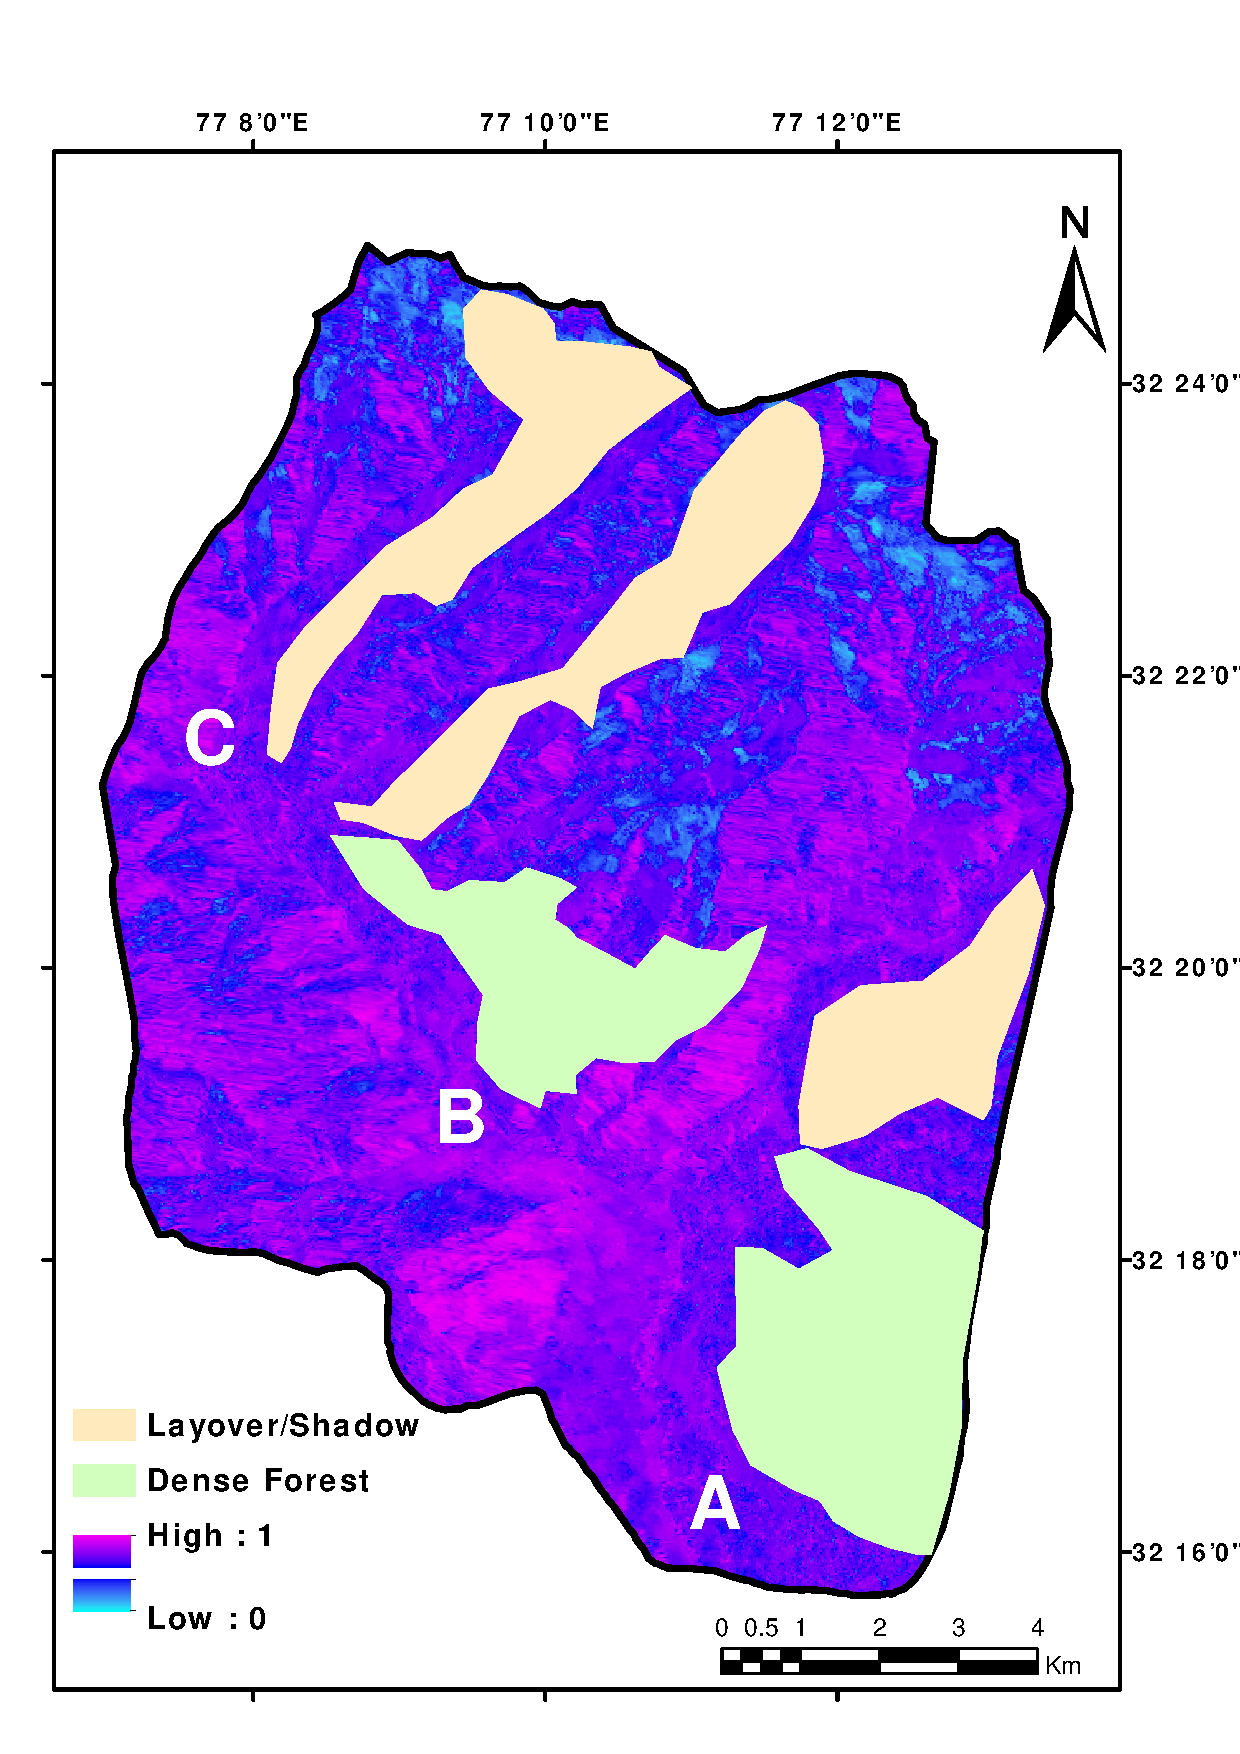
\includegraphics[width=0.4\columnwidth]{Figures_SSD/Ag4U_DOP}} 
	\hspace{1mm}
	\subfloat[]{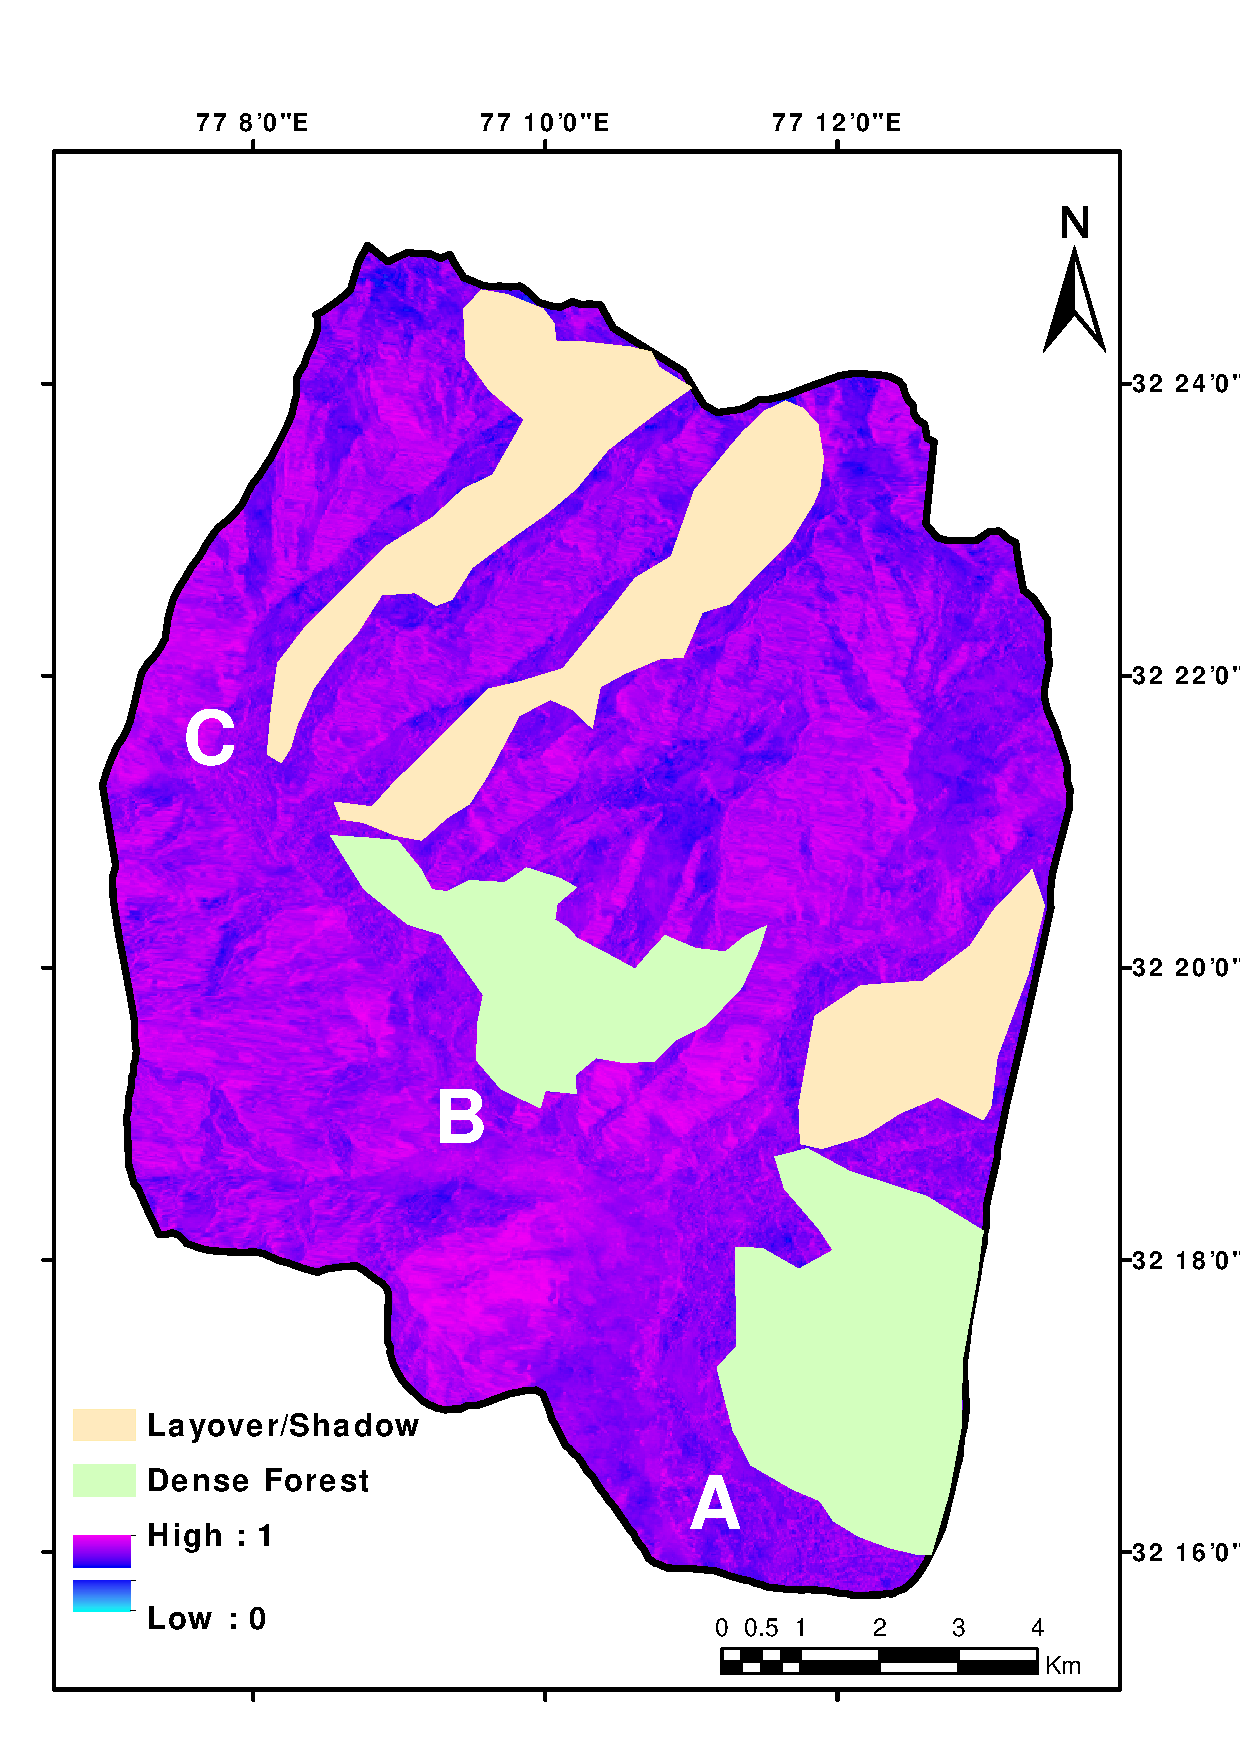
\includegraphics[width=0.4\columnwidth]{Figures_SSD/Touzi_DOP}} 
	\vspace{1mm}
	\subfloat[]{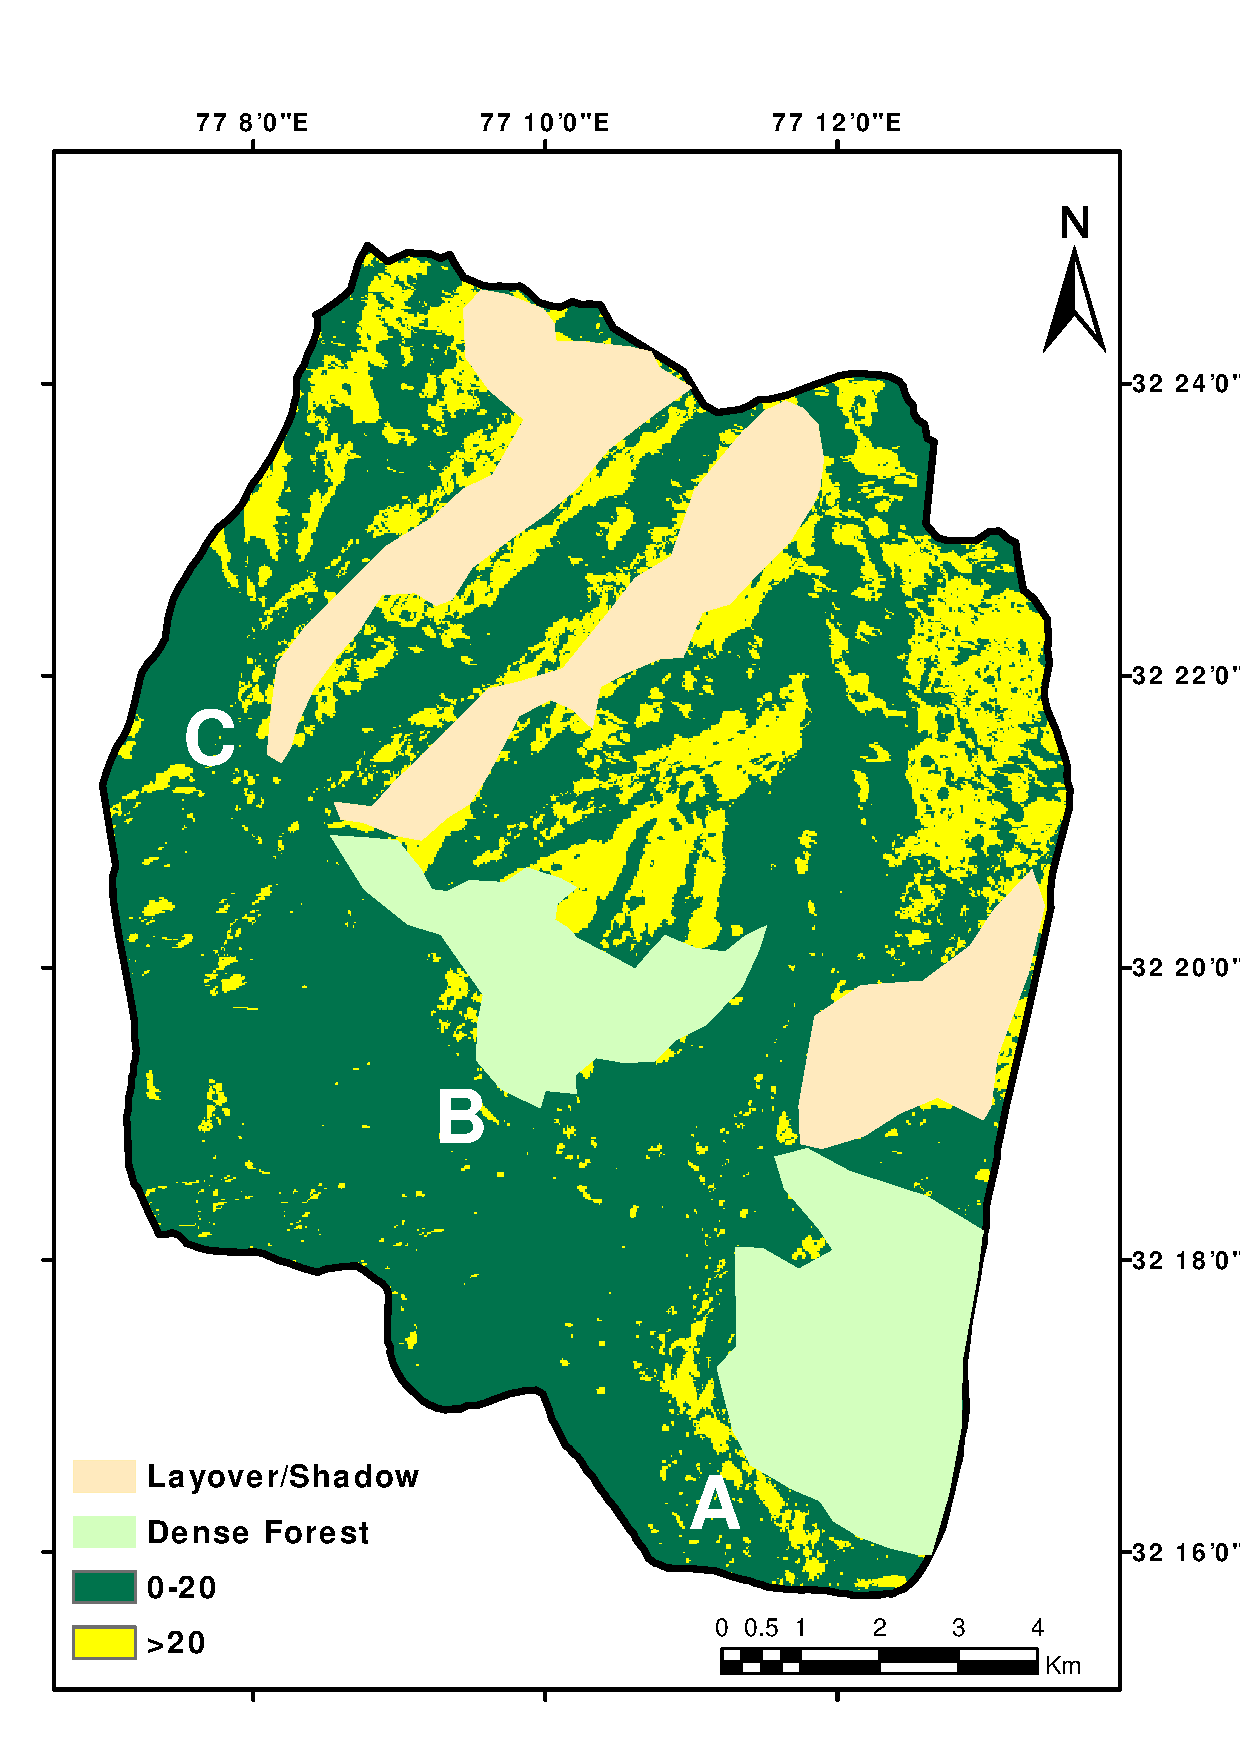
\includegraphics[width=0.4\columnwidth]{Figures_SSD/alpha_8feb13}} \hspace{1mm}
	\subfloat[]{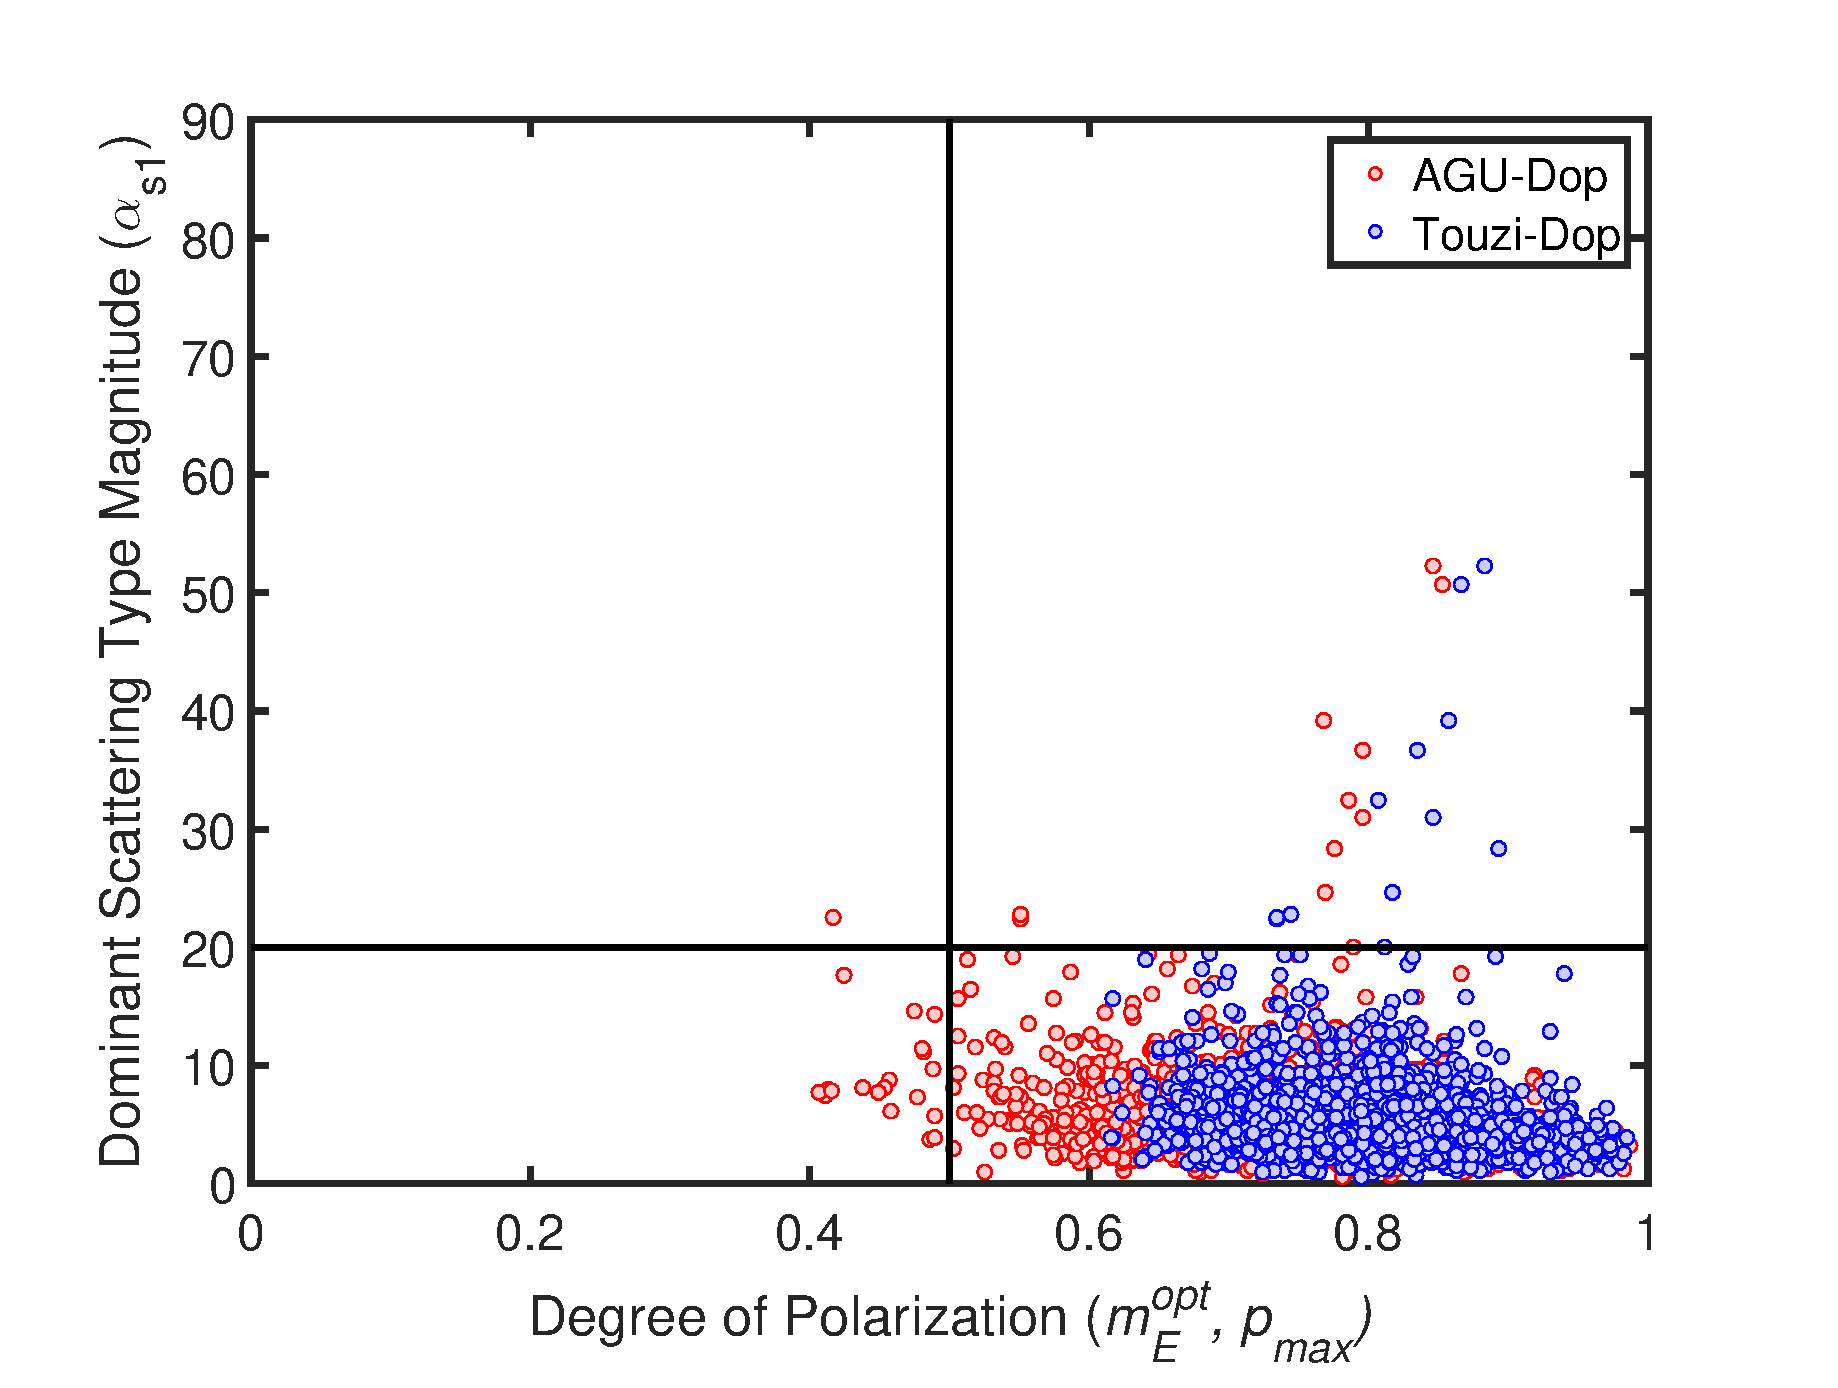
\includegraphics[width=0.4\columnwidth]{Figures_SSD/dop_alpha_1}} 
	\caption[The optimum degree of polarization by (a) AGU (b) Touzi methods, (c) the dominant scattering type magnitude and (d) the $\alpha_{s1} \mbox{vs.} m_{E}^{\mbox{\scriptsize opt}}$ plot for 8 Feb.2013 data]{The optimum degree of polarization by (a) AGU and (b) Touzi methods, (c) the dominant scattering type magnitude and (d) the $\alpha_{s1} \mbox{vs.} m_{E}^{\mbox{\scriptsize opt}}$ plot for 8 Feb.2013 data. The points A, B and C on the maps are the three observatory locations over the study area.}
	\label{fig:results_1}
\end{figure*}
%\begin{figure*}[!h]
%	\centering
%	\subfloat[$m_{E}^{\mbox{\scriptsize opt}}$\label{Fig:AGU_DOP}]{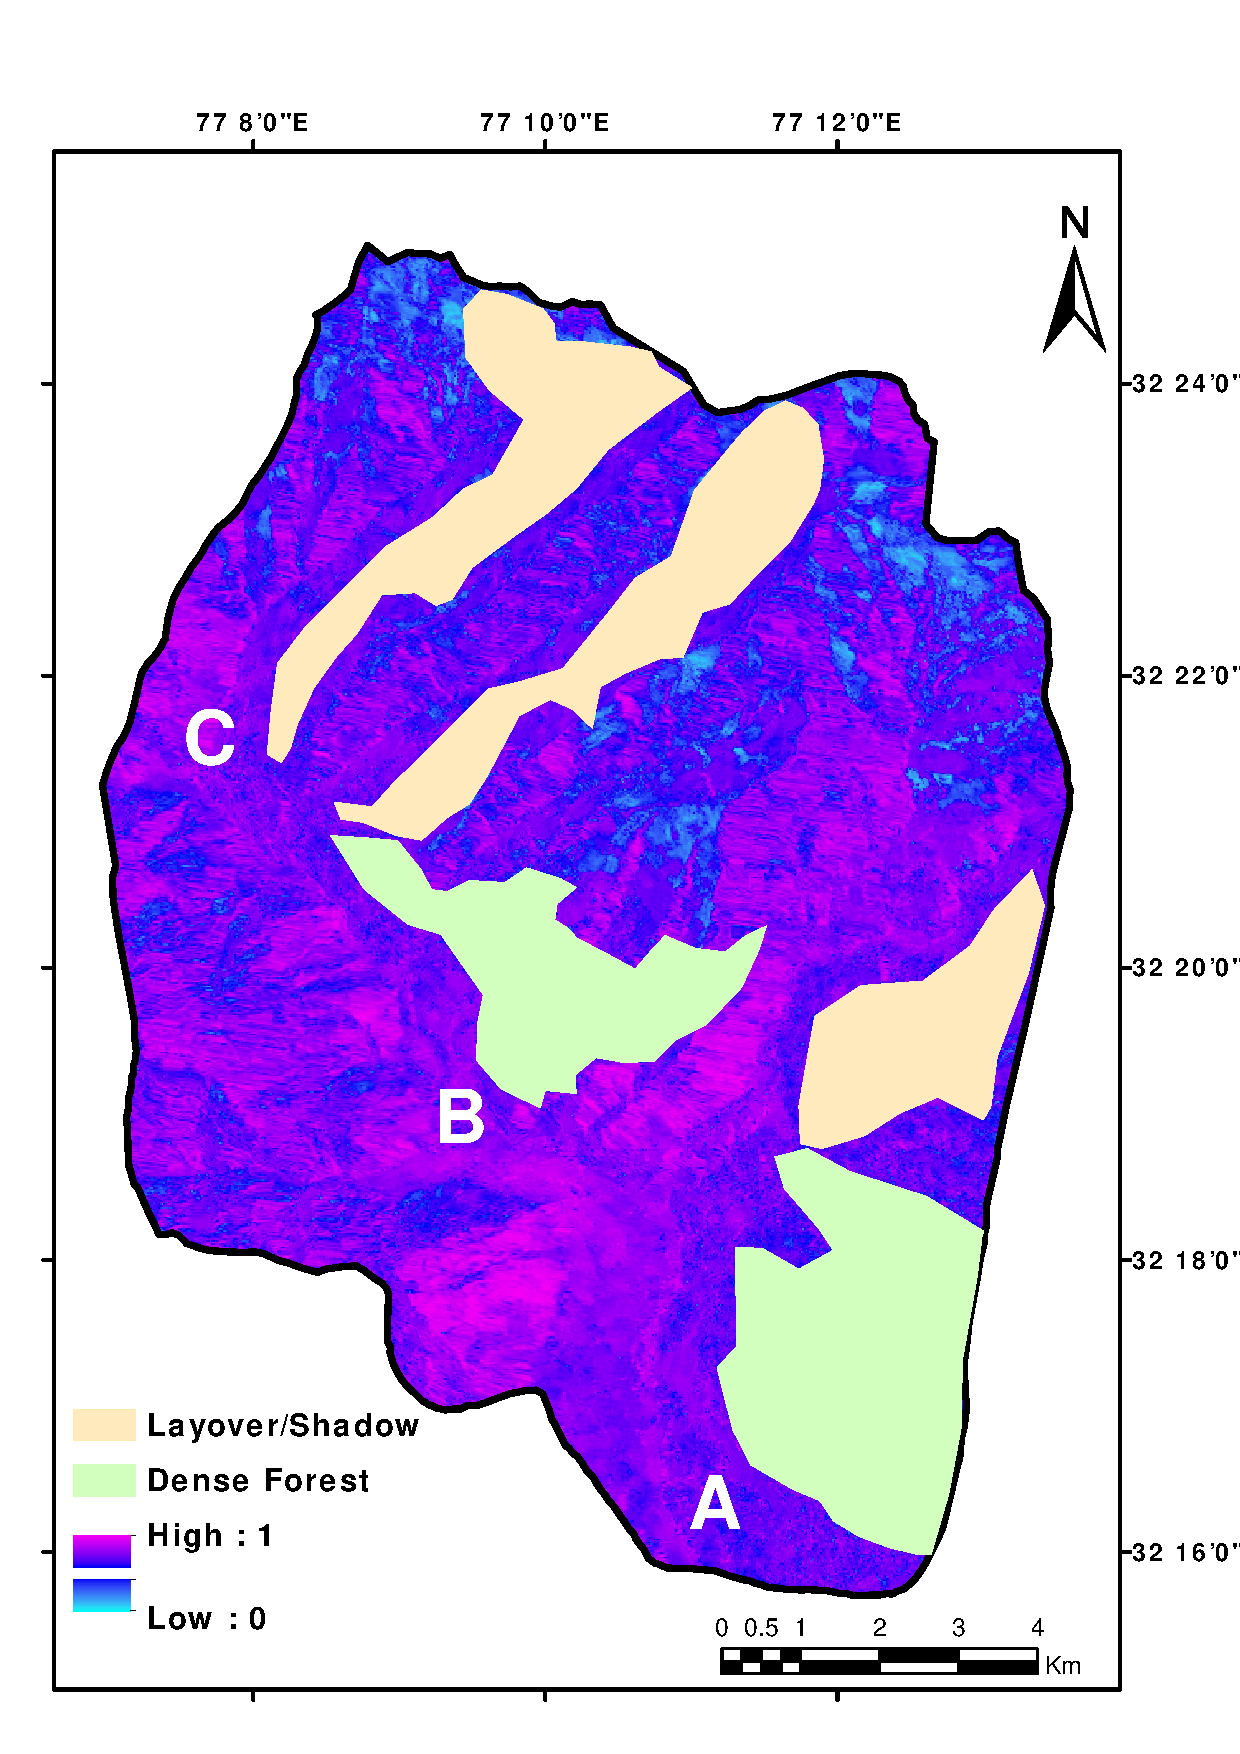
\includegraphics[width=0.4\columnwidth]{Figures_SSD/Ag4U_DOP}} 
%	\hspace{1mm}
%	\subfloat[$p_{max}$\label{Fig:Touzi_DOP}]{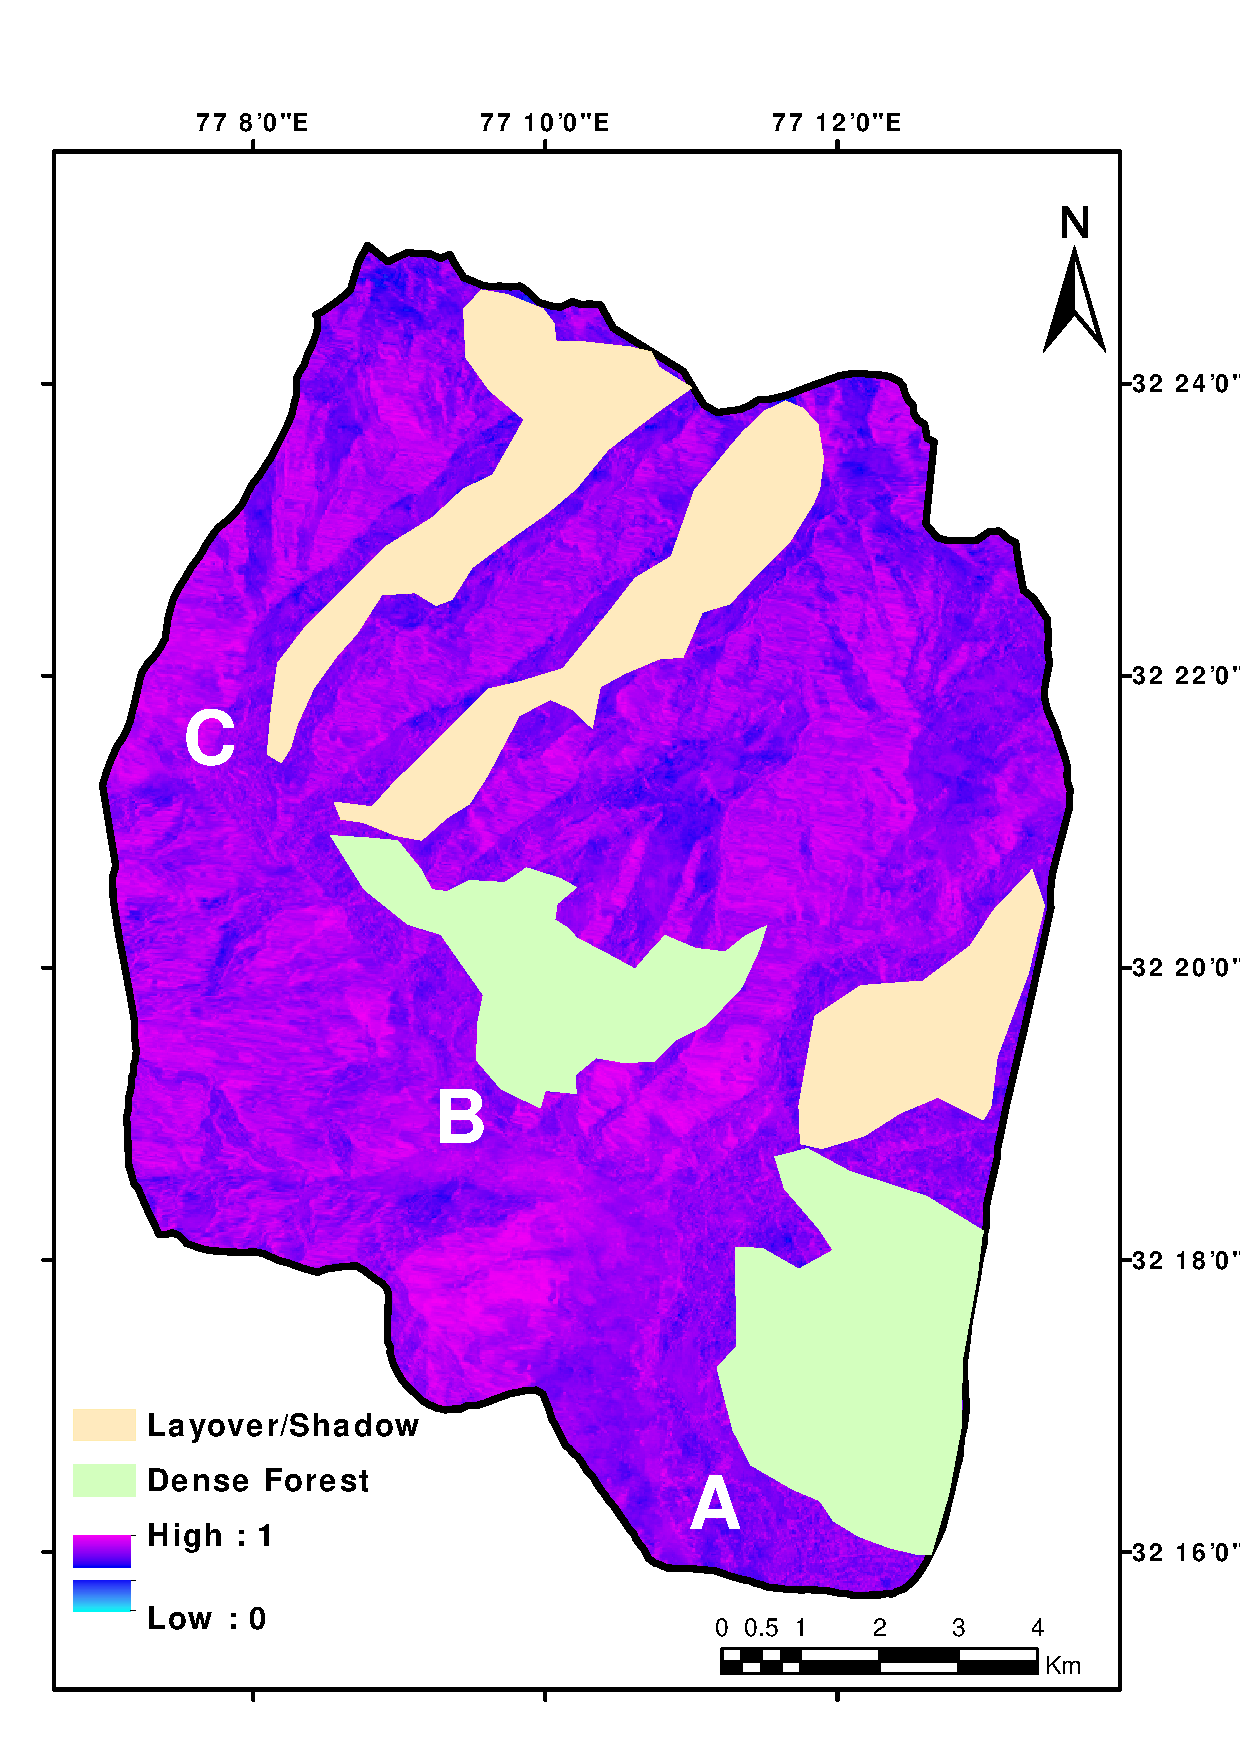
\includegraphics[width=0.4\columnwidth]{Figures_SSD/Touzi_DOP}} 
%	\vspace{1mm}
%	\subfloat[$\alpha_{s1}$\label{Fig:alpha_s1}]{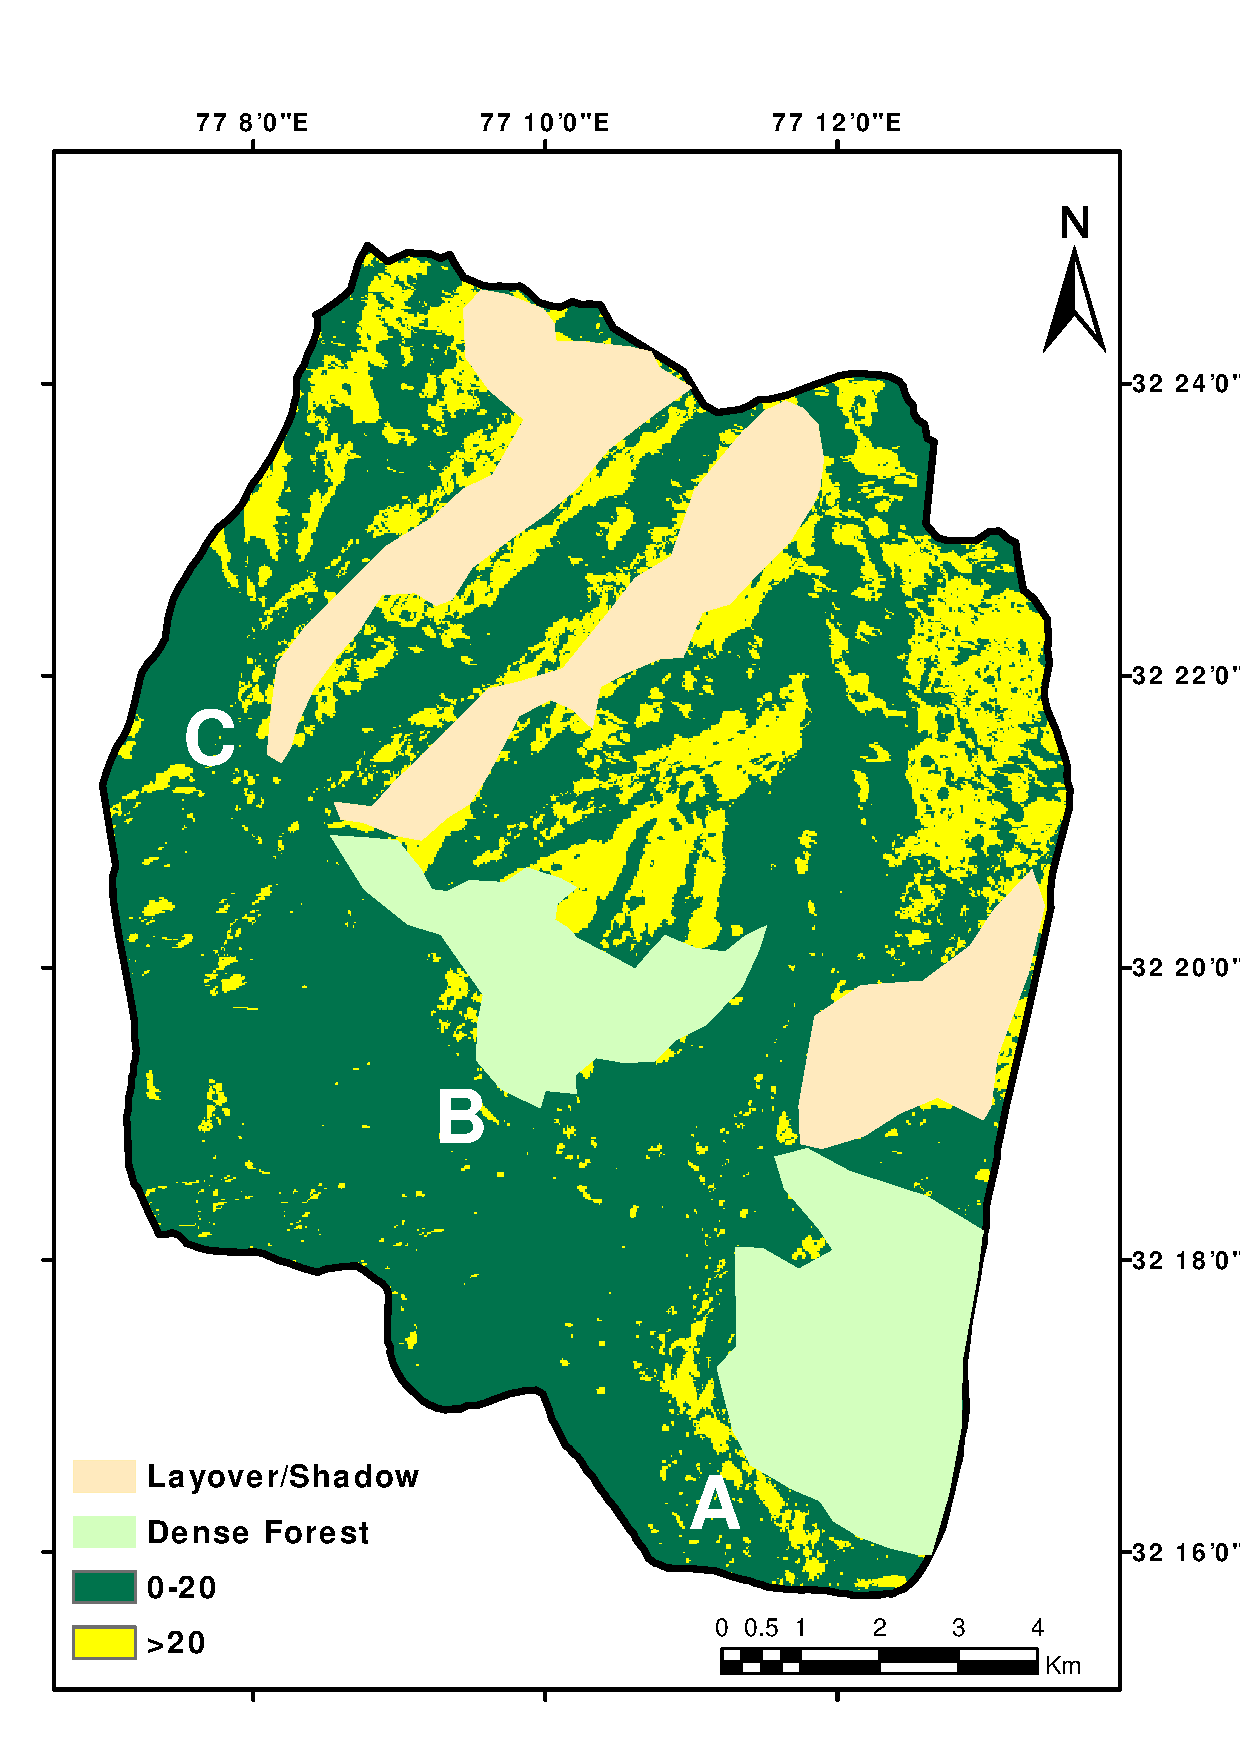
\includegraphics[width=0.4\columnwidth]{Figures_SSD/alpha_8feb13}} \hspace{1mm}
%	\subfloat[$\alpha_{s1} \mbox{vs.} Dop$\label{Fig:dop_alpha}]{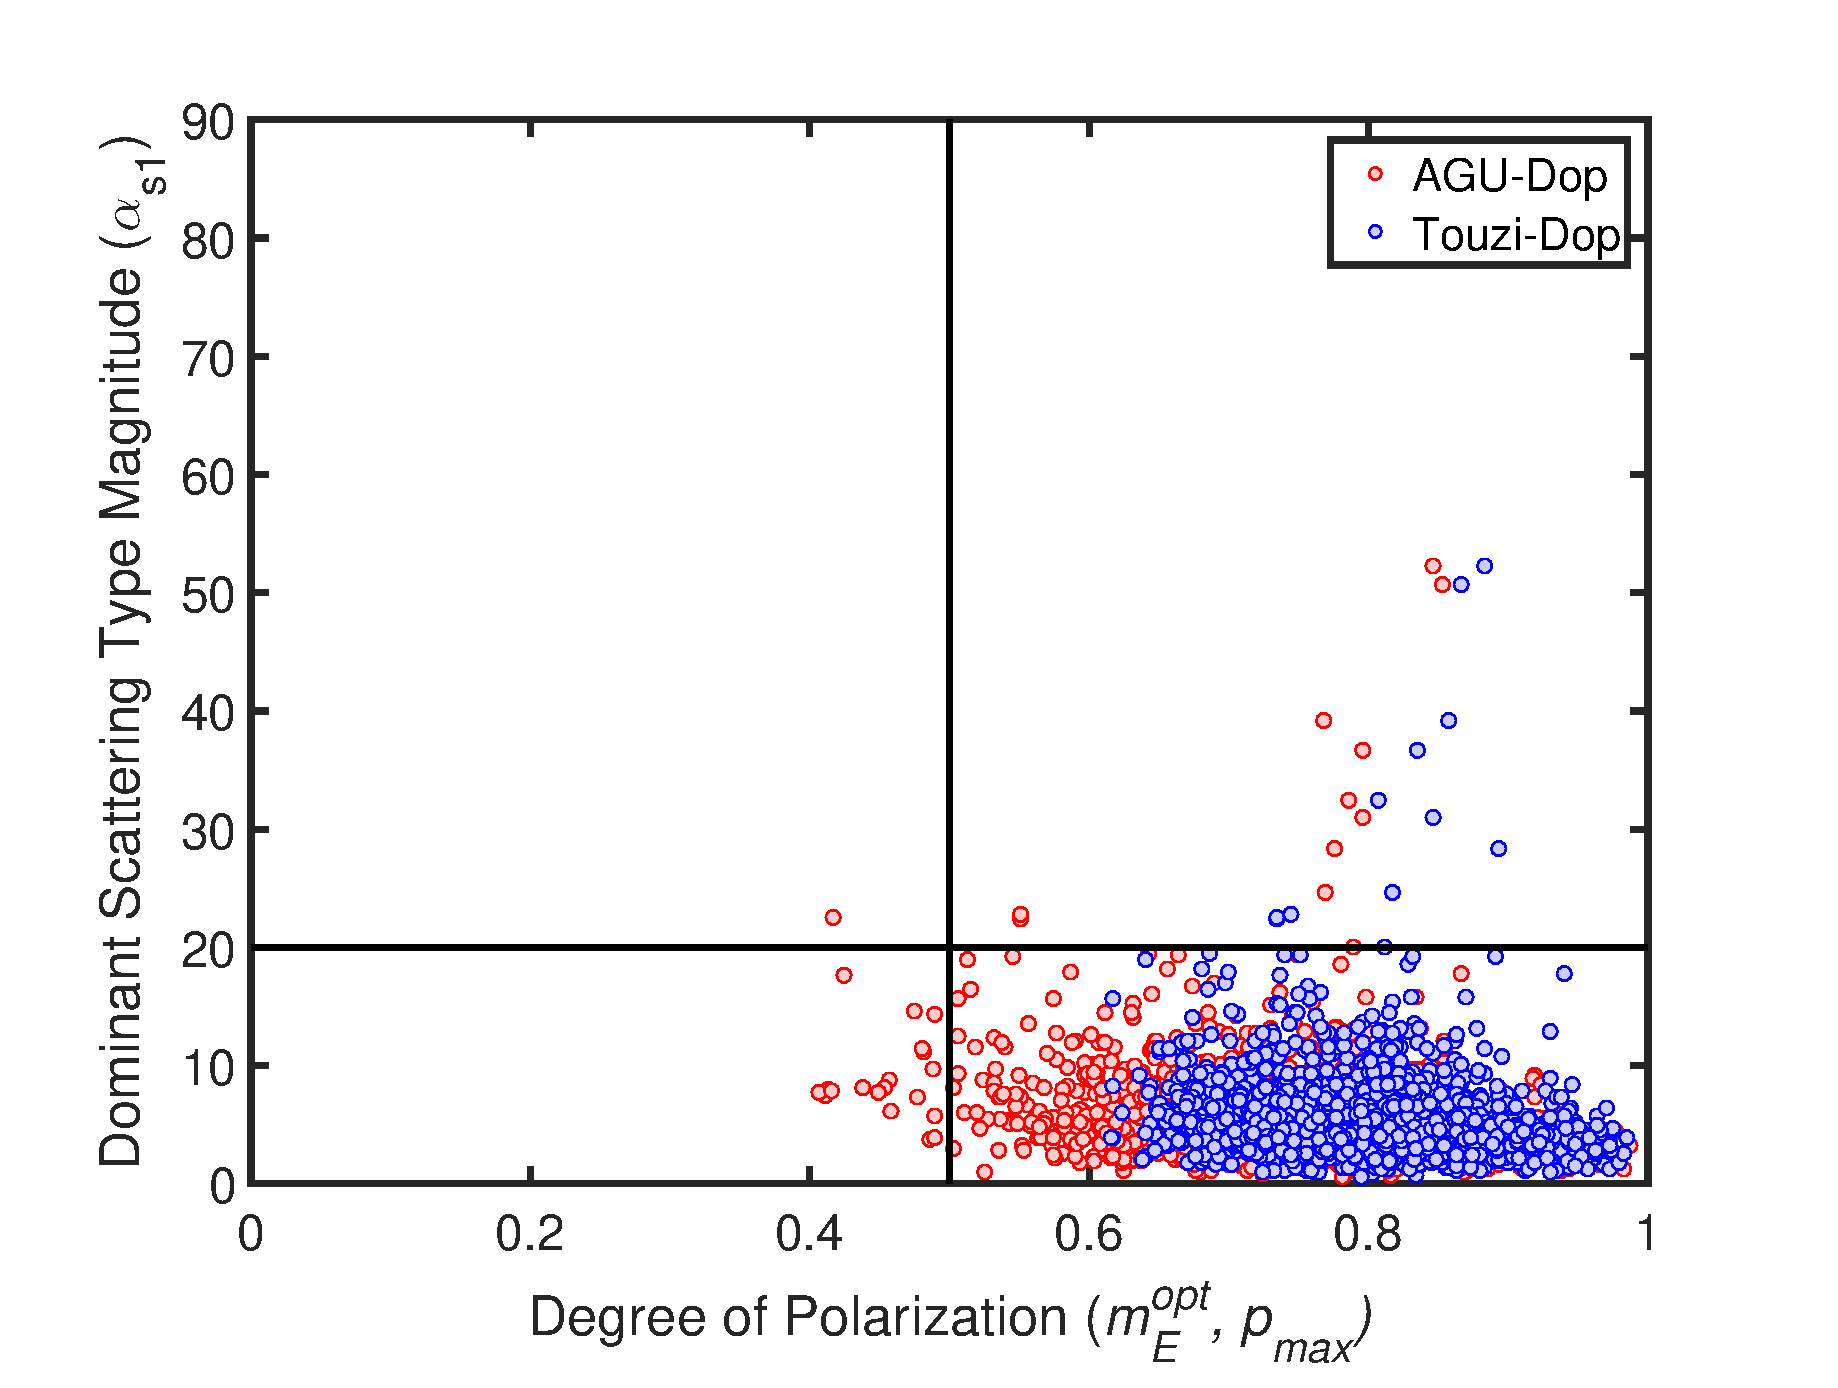
\includegraphics[width=0.4\columnwidth]{Figures_SSD/dop_alpha_1}} 
%	\caption[The optimum degree of polarization by (a) AGU and (b) Touzi methods, (c) The dominant scattering type magnitude (d) the $\alpha_{s1} \mbox{vs.} m_{E}^{\mbox{\scriptsize opt}}$ plot for 8 Feb.2013 data]{The optimum degree of polarization by (a) AGU and (b) Touzi methods, (c) The dominant scattering type magnitude (d) the $\alpha_{s1} \mbox{vs.} m_{E}^{\mbox{\scriptsize opt}}$ plot for 8 Feb.2013 data. The points A, B and C on the maps are the three observatory locations over the study area.}
%	\label{fig:results_1}
%\end{figure*}

\subsection{Snow surface dielectric constant}
The small perturbation or Bragg rough surface scattering~\citep{tsang1985theory} is defined for large (compared to the incident wavelength $\lambda$) surface facets where the rms surface roughness $s$ is small compared to $\lambda$. This is usually expressed in terms of the wavenumber $k$ and for all practical applications $ks < 0.3$. The backscattered power depends only on a certain frequency component which pertains to the surface roughness spectrum (the Fourier transform of the surface profile). Moreover, the surface roughness is implicit in the Fourier transform of the surface profile and it is similar to both the polarization channels (HH and VV). Hence, a simple ratio of the co-polarized channels (eg. HH/VV) will be only a function of the local incidence angle $\theta_{i}$ and the snow surface dielectric constant $\varepsilon_{r}$~\citep{cloude2009polarisation}. 

The Bragg scattering is considered without the cross-polarization component. The surface roughness criteria in this case is tightly constrained which limits its practical  applicability. In order to circumvent this problem, the extended Bragg (X-Bragg) model was proposed in~\cite{Hajnsek2003}. The scattered field ($\mathbf{E_{pq}^s}$) given in \eqref{eq:scattered_field} is related to the Bragg coefficients $B_{HH}$ and $B_{VV}$ for the co-polarized components~\eqref{eq:bragg_coefficients_1}--~\eqref{eq:bragg_coefficients_2}. These co-polarized components depend only on the local incidence angle $\theta$ and the dielectric constant $\varepsilon_{r}$, whereas the cross-polarized component $B_{HV}=B_{VH}=0$. 
\begin{subequations}
	\begin{align}
	\mathbf{E_{pq}^s} = & i2k\cos\theta B_{pq}\hat{Z}(2k\sin\theta)
	\label{eq:scattered_field} \\
	B_{HH} = & \frac{\mbox{cos}\theta_{i} - \sqrt{\varepsilon_{r} - \mbox{sin}^2\theta_{i}}}{\mbox{cos}\theta_{i} + \sqrt{\varepsilon_{r} - \mbox{sin}^2\theta_{i}}} \label{eq:bragg_coefficients_1}\\
	B_{VV} = & (\varepsilon_{r}-1)\frac{\mbox{sin}^2\theta_{i} - \varepsilon_{r}(1 + \mbox{sin}^2\theta_{i})}{\left[\varepsilon_{r}\mbox{cos}\theta_{i} + \sqrt{\varepsilon_{r} - \mbox{sin}^2\theta_{i}}\right]^2} \label{eq:bragg_coefficients_2} 
	\end{align}
\end{subequations}

Using this model, two independent parameters: roughness index and the moisture index were derived~\citep{cloude2002new}. The roughness index is dependent on the dielectric constant and the angle of incidence, while the moisture index is independent of the roughness and the surface scattering amplitude. It only depends on the dielectric constant $\varepsilon_{r}$ and the angle of incidence $\theta$. The moisture index is used in this study which relates the roll-invariant dominant scattering type amplitude $\alpha_{s1}$ to the Bragg coefficients $B_{HH}$ and $B_{VV}$~\eqref{eq:alphas1_bragg}.
\begin{equation}
\alpha_{s1}=\tan^{-1}\Bigg(\Bigg|\frac{B_{HH}-B_{VV}}{B_{HH}+B_{VV}}\Bigg|\Bigg), \quad \alpha_{s1} \in \alpha_{s1}^{B}
\label{eq:alphas1_bragg}
\end{equation}
%\begin{subequations}
%	\begin{align}
%	B_{HH} =& \frac{\mbox{cos}\theta_{i} - \sqrt{\varepsilon_{r} - \mbox{sin}^2\theta_{i}}}{\mbox{cos}\theta_{i} + \sqrt{\varepsilon_{r} - \mbox{sin}^2\theta_{i}}} \label{eq:bragg_coefficients_1}\\
%	B_{VV} =& (\varepsilon_{r}-1)\frac{\mbox{sin}^2\theta_{i} - \varepsilon_{r}(1 + \mbox{sin}^2\theta_{i})}{\left[\varepsilon_{r}\mbox{cos}\theta_{i} + \sqrt{\varepsilon_{r} - \mbox{sin}^2\theta_{i}}\right]^2} \label{eq:bragg_coefficients_2}
%	\end{align}
%\end{subequations}

Following this, the snow surface dielectric constant $\varepsilon_{r}$ is numerically obtained by inverting~\eqref{eq:alphas1_bragg} for only those pixels which lie in the region of $\alpha_{s1}^{B}$ and $m_{E}^{\mbox{\scriptsize opt}} > 0.5$. This can be clearly seen in Figure~\ref{fig:results_1}(d) for samples from the study area used in this paper for the 8 Feb data. This methodology can be justified by the fact that approximately $9-10\%$ increase in the number of pixels have been obtained as compared to the original data $(\langle[{\mathbf{T}}]\rangle)$, for all the data sets used in this study by using the criteria of optimum degree of polarization $m_{E}^{\mbox{\scriptsize opt}}$. These pixels lie in the region of $\alpha_{s1}^{B}$ and have been correctly inverted to obtain $\varepsilon_{r}$. 

\section{Snow density estimation using full polarimetric SAR data}
\label{sec:3.4}
Followed by the snow wetness estimation from full polarimetry SAR data~\ref{sec:3.2}, here also the general four-component scattering power decomposition method (G4U)~\citep{singh13} is adopted to develop a new snow density estimation method. The G4U decomposition which is used in this study, has the added advantage of full utilization of the polarimetric coherency phase information provided by a full-polarimetric SAR data. Unlike the L-band data, the estimation of the snow density using C-band relies mainly on the scattering from the snowpack volume. Therefore, the generalized volume parameter is utilized in this study. It is then directly used to invert the snowpack dielectric constant. The effective snow dielectric constant is derived using the normalized volume scattering power, which is then used in a standard semi-empirical equation~\citep{looyenga1965dielectric} to estimate the snow density. 

%Unlike the Freeman-Durden decomposition (FDD)~\citep{freeman98}, the Yamaguchi 4-component decomposition (Y4O)~\citep{Yamaguchi05} and the Yamaguchi 4-component decomposition with rotation (Y4R)~\citep{YAMAGUCHI2011}, which only uses 55.5$\%$, 66.6$\%$ and 75$\%$ of the polarimetric phase information respectively whereas the G4U utilizes 100$\%$ of the polarimetric phase information which is implemented by a double unitary transformation of the coherency matrix~(\ref{eq:g4u_decomposition_1} and~\ref{eq:g4u_decomposition_2}), 
%
%\begin{subequations}
%\begin{multline}
% \left\langle\mathbf{[T(\theta)]}\right\rangle = \left[U(\theta)\right]\Bigl(f_{s}\left\langle\mathbf{[T]}\right\rangle_{surface} +  f_{d}\left\langle\mathbf{[T]}\right\rangle_{double} + f_v\left\langle\mathbf{[T]}\right\rangle_{vol} \\ + f_{c}\left\langle\mathbf{[T]}\right\rangle_{helix}\Bigr)\left[U(\theta)\right]^{\dagger}
%\label{eq:g4u_decomposition_1}
%\end{multline}
%\begin{equation}
%\left\langle\mathbf{[T(\phi)]}\right\rangle = \left[U(\phi)\right]\left\langle\mathbf{[T(\theta)]}\right\rangle\left[U(\phi)\right]^{\dagger} = \left[ \begin{array}{ccc}
%T_{11} & T_{12} & T_{13} \\
%T_{21} & T_{22} & 0 \\
%T_{31} & 0 & T_{33}
%\end{array}\right] 
%\label{eq:g4u_decomposition_2}
%\end{equation}
%\begin{equation}
%\left[U(\theta)\right] = \left[ \begin{array}{ccc}
%1 & 0 & 0 \\
%0 & \mbox{cos}2\theta & \mbox{sin}2\theta \\
%0 & -\mbox{sin}2\theta & \mbox{cos}2\theta
%\end{array}\right];  \quad
%\left[U(\phi)\right] = \left[ \begin{array}{ccc}
%1 & 0 & 0 \\
%0 & \mbox{cos}2\phi & j\mbox{sin}2\phi \\
%0 & j\mbox{sin}2\phi & \mbox{cos}2\phi
%\end{array}\right]
%\label{eq:utheta_and_uphi}
%\end{equation}
%\end{subequations}
%where $\dagger$ denotes complex conjugation and transposition, $\left[U(\theta)\right]$ and $\left[U(\phi)\right]$ denotes the real and the complex unitary transformation matrices respectively~(\ref{eq:utheta_and_uphi}) and $\left\langle\mathbf{[T(\theta)]}\right\rangle = \left[U(\theta)\right]\left\langle\mathbf{[T]}\right\rangle\left[U(\theta)\right]^{\dagger}$ denotes the measured coherency matrix after real orientation compensation. The $f_{s}$, $f_d$, $f_v$ and $f_{c}$ are the corresponding scattering coefficients of the expansion matrices, $\left\langle\mathbf{[T]}\right\rangle_{surface}$, $\left\langle\mathbf{[T]}\right\rangle_{double}$, $\left\langle\mathbf{[T]}\right\rangle_{vol}$ and $\left\langle\mathbf{[T]}\right\rangle_{helix}$ respectively. These coefficient are then used to estimate the surface ($P_s$), double-bounce ($P_d$), volume ($P_v$) and the helix ($P_c$) scattering powers. 
%In this work the scattering by snow particles is modeled in terms of their polarizability.The volume scattering matrix defined for a single particle is defined as,
%\begin{equation}
%[S_{vol}]=\left[\begin{array}{cc}
%S_{HH}^{vol} & 0 \\
%0 & S_{VV}^{vol}
%\end{array}\right] = S_{HH}^{vol}\left[\begin{array}{cc}
%1 & 0 \\
%0 & A_{p}
%\end{array}\right]
%\label{eq:scattering_matrix_fung_sd}
%\end{equation}
%where $A_{p}$ is known as the particle anisotropy.The anisotropy can also be interpreted in terms of the particle geometry and can be defined as the ratio of the principal values of polarizability~\cite{cloude2009polarisation}. In general, the anisotropy parameter can be used to a certain degree of reliability as a reference for the particle shape. However, the anisotropy parameter is also bounded by the dielectric constant ($\varepsilon$) of the particle and is bounded by,
%\begin{equation}
%\frac{1}{\varepsilon{'}_{v}}<A_{p}<\frac{\varepsilon{'}_{v} + 1}{2}.
%\label{eq:anisotropy_sd}
%\end{equation}
%In order to have a volume scattering from a random cloud of snow particles, the volume scattering matrix defined in~(\ref{eq:scattering_matrix_fung_sd}) should be arbitrarily rotated about the line of sight by an angle $\theta$ as,
%\begin{equation}
%[S_{vol}]=S_{HH}^{vol}\left[\begin{array}{cc}
%\mbox{cos}(\theta) & \mbox{sin}(\theta) \\
%-\mbox{sin}(\theta) & \mbox{cos}(\theta)
%\end{array}\right]\left[\begin{array}{cc}
%1 & 0 \\
%0 & A_{p}
%\end{array}\right]\left[\begin{array}{cc}
%\mbox{cos}(\theta) & -\mbox{sin}(\theta) \\
%\mbox{sin}(\theta) & \mbox{cos}(\theta)
%\end{array}\right].
%\label{eq:rotated_volume_scattering_matrix_sd}
%\end{equation}
%for which the volume coherency matrix $[T(\theta)]_{vol}$ can be written as,
%\begin{equation}
%[T(\theta)]_{vol}=\frac{1}{2}\left|S_{HH}^{vol}\right|^2\left[\begin{array}{ccc}
%|1+A_{p}|^2 & (1 + A_{p})\mbox{cos}2\theta & -(1 + A_{p})\mbox{sin}2\theta    \\
%(1 + A_{p})^*\mbox{cos}2\theta & |1-A_{p}|^2\mbox{cos}^22\theta  & -|1-A_{p}|^2\frac{\mbox{sin}4\theta}{2}   \\ 
%-(1 + A_{p})^*\mbox{sin}2\theta & -|1-A_{p}|^2\frac{\mbox{sin}4\theta}{2} & |1-A_{p}|^2\mbox{sin}^22\theta
%\end{array}\right].
%\label{eq:coh_matrix_sp_sd}
%\end{equation}
%The volume scattering coherency matrix in~(\ref{eq:coh_matrix_sp_sd}) is averaged over all possible angles $\theta$ to obtain the volume scattering coherency matrix of a random cloud of small spheroid particles in one resolution cell as,
%\begin{equation}
%\left\langle[T]\right\rangle_{vol}^{snow}=\int[T(\theta)]_{vol}p(\theta)d\theta
%\label{eq:average_coherency_matrix_sd}
%\end{equation}
%for uniformly distributed snow particles, 
%\begin{equation}
%p(\theta)=\frac{1}{2\pi} \quad; 0<\theta<2\pi
%\label{eq:uniform_distrbn_sd}
%\end{equation}
%The average snow volume coherency matrix~(\ref{eq:volume_coherency_matrix_sd}) can be written in terms of generalized volume parameter ($|\gamma|^2$), 
%\begin{equation}
%\left\langle\mathbf{[T]}\right\rangle_{vol}^{snow} = f_{v}\left[ \begin{array}{ccc}
%|\gamma|^{2} & 0 & 0 \\
%0 & \frac{1}{2} & 0 \\
%0 & 0 & \frac{1}{2}
%\end{array}\right].
%\label{eq:volume_coherency_matrix_sd}
%\end{equation}
%with the volume scattering coefficient as,
%\begin{equation}
%f_{v} = \frac{1}{2}|\gamma_{HH}-\gamma_{VV}|^{2}f(\theta_{i},\theta_{r},\omega,\tau,P)
%\label{eq:fv_sw}
%\end{equation}
%where $\theta_{i}$ and $\theta_{r}$ are the local incidence and refractive angles, $\omega=\kappa_{s}/\kappa_{e}$ is the snow volume albedo, defined as the ratio of the scattering $\kappa_{s}$ and the extinction coefficient $\kappa_{e}$, $\tau$ is the optical depth ($\tau=\kappa_{e}d$) where $d$ is the snow depth, $P$ is the Rayleigh scattering phase function and,
%\begin{equation}
%|\gamma|^2 = \frac{|\gamma_{HH} + \gamma_{VV}|^2}{|\gamma_{HH} - \gamma_{VV}|^2} = \frac{|1 + A_{p}|^2}{|1 - A_{p}|^2}.
%\label{eq:gammasquare_sd}
%\end{equation}
%where $\gamma_{HH}$ and $\gamma_{VV}$ are the Fresnel transmission coefficients for HH and VV polarizations respectively,
%\begin{subequations}
%	\begin{align}
%	\gamma_{HH} =& \frac{2\sqrt{\varepsilon{'}_{v} - \mbox{sin}^2\theta_{i}}}{\mbox{cos}\theta_{i} + \sqrt{\varepsilon{'}_{v} - \mbox{sin}^2\theta_{i}}} \\
%	\gamma_{VV} =& \frac{2\sqrt{\varepsilon{'}_{v} - \mbox{sin}^2\theta_{i}}}{\varepsilon{'}_{v}\mbox{cos}\theta_{i} + \sqrt{\varepsilon{'}_{v} - \mbox{sin}^2\theta_{i}}}
%	\end{align}
%	\label{eq:fresnel_trans_coefficients_sd}
%\end{subequations}
%the local incidence angle $\theta_{i}$ should be converted into the local refractive angle $\theta_{r}$ using the Snell's law.
%%Since $A_{p}$ is bounded, therefore $|\gamma|^2$ is also bounded as,
%%\begin{equation}
%%\left|\frac{\varepsilon_{v}+1}{\varepsilon_{v}-1}\right|^2 < |\gamma|^2 < \left|\frac{\varepsilon_{v}+3}{\varepsilon_{v}-1}\right|^2
%%\end{equation}
%By assuming that the double-bounce scattering is negligible in wet snow, the generalized volume parameter $|\gamma|^2$ is derived~\cite{singh2013b} as,
%\begin{equation}
%|\gamma|^2 = \frac{T_{11}(\theta)}{2T_{33}(\theta)-f_c} - \frac{|T_{12}(\theta)+T_{13}(\theta)|^{2}}{(2T_{33}(\theta)-f_{c})(T_{22}(\theta)-T_{33}(\theta)}
%\label{eq:gamma_square_coherency_elememts_sd}
%\end{equation}
%where $f_{c}$ is the helix scattering coefficient given as,
%\begin{equation}
%f_{c}=2|\mbox{Im}\{T_{23}(\theta)\}|.
%\label{eq:helix_scattering_coefficient_sd}
%\end{equation}
%The snow volume dielectric constant is then estimated by equating~(\ref{eq:gammasquare_sd}) and~(\ref{eq:gamma_square_coherency_elememts_sd}).
The generalized volume parameter ($|\gamma|^2$) derived from~(\ref{eq:gamma_square_coherency_elememts_sw}) is equated with~(\ref{eq:gammasquare_sw}) for the inversion of snowpack volume dielectric constant. The estimated snowpack volume dielectric constant is normalized with the volume scattering power ($\omega=P_v/TP$) estimated from the G4U decomposition. This normalized (effective) snowpack dielectric constant ($\varepsilon_{e}{'}=\omega.\varepsilon_{v}{'}$) is then used in the Looyenga's semi-empirical dielectric equation~\citep{looyenga1965dielectric} to estimate the snow density ($\rho_s$). The flowchart of the proposed methodology is shown in Figure~\ref{fig:methodology}. 

\begin{equation}
\varepsilon_{e}{'}=1.0 + 1.5995\rho_s + 1.861\rho_s^{3}
\label{eq:looyenga}
\end{equation}

\begin{sidewaysfigure}
	\centering
	\includegraphics[width=0.49\textwidth]{Figures_sd/flow_chart}
	\caption [Flowchart of snow density estimation algorithm]{Flowchart of the snow density estimation method for C-band full polarimetric data}
	\label{fig:methodology}
\end{sidewaysfigure}

In this proposed method, the generalized volume parameter utilizes the full-polarimetric SAR measurements from the snowpack. Hence, this parameter is able to take care of various snow conditions. On the other hand, the scattering powers from the snowpack volume is a function of the penetration depth, the grain size, the snow wetness, etc. So, the generalized volume parameter combined with the scattering power is able to correctly quantify the snowpack density. During February, in the Indian Himalayan region, more than 90 $\%$ of the study area was completely covered with snow and our method was directly applied to the area. There was no masking used in this study to classify a area into wet/dry snow/snow free. The classification of wet or dry snow was not required because the proposed model takes into account different scattering mechanism contribution associated with different snow conditions while calculating the effective density.
\chapter{Results and Discussions}
\label{sec:4}
In this Chapter, the results obtained from all the algorithms are presented in separate sub-sections along with the detailed investigations using topographic and observatory measurements. Multi-temporal analyses of the results are also presented. 
\section{Snow wetness from dual polarimetric data}
\FloatBarrier
In this section, the results obtained from the proposed snow wetness estimation method for dual-polarimetric coherent (HH/VV) SAR data (\emph{i.e.,} TerraSAR-X)~\cref{sec:3.1} are presented. This method is based on the work of~\cite{jagdhuber2013polarimetric} for soil moisture estimation. The dominant surface and volume scatterings for the wet snow lead us to estimate the snow surface and snowpack volume wetness. The snow surface wetness is estimated by using the simplified IEM model for high frequency limit of X-band (9.6 GHz) data. The snow volume wetness is estimated under the Rayleigh scattering assumption. The proposed method is used to estimate the snow wetness of the top layers of the snowpack. The results obtained from the proposed method are validated using the near real time in-situ measurements with the satellite pass.
\subsection{Study area and data used}
\label{sec:4.1.1}
The field campaign was conducted to collect the in-situ measurements synchronized with the TerraSAR-X data acquisition on 23 January 2009 (the area outline in blue in Figure~\ref{fig:study_area_dual_pol}). Along with this dataset, three more TerraSAR-X datasets acquired on 12 January 2009, 18 January 2009 and 24 January 2009 (the area outlined as red in Figure~\ref{fig:study_area_dual_pol}) have also been used to infer the snow wetness changes over the study area. The Solang observatory, where the field campaign was conducted is marked (green star) in Figure~\ref{fig:study_area_dual_pol}. The date, time of acquisition, pass and incidence angles of the data used in this study are given in Table~\ref{table:data acquisition_sw_dual}.
\begin{table}[!htbp]
	\caption{TerraSAR-X data acquisition table}
	\begin{center}
		\begin{tabular}{| c | c |c | c |c |} \hline
			No & Date & Acq. Time (IST) & Pass & Inc. Angle ($^\circ$) \\ \hline \hline
			1 & 12 Jan 2009 & 6:14 AM & Des & 38.3-39.4\\ \hline
			2 & 18 Jan 2009 & 6:24 PM & Asc & 47.3-48.2\\ \hline
			3 & 23 Jan 2009 & 6:24 AM & Des & 38.1-39.1\\ \hline
			4 & 24 Jan 2009 & 6:15 PM & Asc & 32.1-33.3\\ \hline
		\end{tabular}
	\end{center}
	\label{table:data acquisition_sw_dual}
\end{table}
The in-situ snow wetness was measured with a dielectric moisture meter~\citep{denoth1989snow,denoth1995electron}. The snow probe was used for measuring the permittivity$\varepsilon$) of the snow medium. The volumetric liquid water content ($W(\mbox{Vol}\%)$) was calculated from the measured snow permittivity ($\varepsilon$) and the snow density ($\rho$), using the following empirical relation~\citep{denoth1995electron}:
\begin{equation}
W(\mbox{Vol}\%)=5.35\left[\varepsilon-(1+1.92\rho)\right]
\label{eq:denoth}
\end{equation}

\begin{figure}[!htbp]
	\centering
	\includegraphics[width=\columnwidth]{Figures/study_area_sw_dual}
	\caption [Study area of Solang, Himachal Pradesh, India]{Study area along with the footprints of the TerraSAR-X acquisitions. The Solang observatory is indicated by a green star in the image.}
	\label{fig:study_area_dual_pol}	
\end{figure}

The snow wetness map for the 23 Jan. 2009 data, estimated by the proposed method is shown in Figure~\ref{fig:proposed_results_dualpol}(c). It can be seen that major part of the study area exhibits wetness in the range of 0-4$\%$ by volume. This data was acquired in descending pass and the temperature recorded during the pass was around 2.5$^\circ$C. At some places the estimated wetness is in the range of $>$5$\%$ by volume. This could be possible due to a slight amount of rainfall (5.8~mm) over the Solang valley which is evident from the observatory data (Table~\ref{table:observatory_data_dual_pol}). Since the snow temperature is lower than the downpour water, the snow has absorbed the downpour water temperature and began to melt. However, there are blanks (white pixels) in the right hand side of the wetness map. This could be because of geometric distortions (possibly shadow) due to a slope facing away from the radar. All images with descending passes used in this study have similar blank portions. The snow wetness results estimated by the proposed method for this dataset is compared with the in-situ measurements Figure~(\ref{fig:validation_plot_dualpol}). It can be seen that the estimated snow wetness by the proposed method are closer to the in-situ measurements. The overall mean absolute error for the proposed method is 1.65$\%$ by volume.

\begin{figure}[!htbp]
	\centering
	\subfloat[]{\includegraphics[width=0.5\textwidth]{Figures_SW2/12Jan}} 
	\subfloat[]{\includegraphics[width=0.5\textwidth]{Figures_SW2/18Jan}} \\
	\subfloat[]{\includegraphics[width=0.5\textwidth]{Figures_SW2/23Jan}}
	\subfloat[]{\includegraphics[width=0.5\textwidth]{Figures_SW2/24Jan}}
	\caption [Snow wetness maps from TerraSAR-X dual coherent PolSAR data]{Snow wetness maps from TerraSAR-X dual coherent PolSAR data derived from the proposed method.} 
	\label{fig:proposed_results_dualpol}
\end{figure}

The proposed snow wetness estimation method is also applied to three other TerraSAR-X datasets acquired during the same season (12, 18 and 24 Jan. 2009). The snow wetness map for 12 Jan. 2009 shows low values (0-2$\%$) for most of the study area as shown in Figure~\ref{fig:proposed_results_dualpol}(a) which could be due to very low temperature (-3.5$^\circ$C) during the acquisition (descending). On 18 January, there was a snowfall of 13 cm and the maximum temperature recorded for the day (FN and AN) was 4$^\circ$C (Table~\ref{table:observatory_data_dual_pol}). These conditions are reflected in Figure~\ref{fig:proposed_results_dualpol}(b), where most of the area is covered with dry snow. On 24 January, the standing snow has reduced by 7 cm within a span of less than 12 hours with the temperature varying from 4.0 - 10.5$^\circ$C (Table~\ref{table:observatory_data_dual_pol}). The snow wetness is observed to vary from 3-10$\%$ as seen in Figure~\ref{fig:proposed_results_dualpol}(d) due to this temperature variation.

\begin{figure}[!htbp]
	\centering
	\includegraphics[width=\columnwidth]{Figures_SW2/Validation_plot_SW_dual}
	\caption [Validation of snow wetness method for dual pol data]{Comparison of the estimated snow wetness by the proposed method with the in-situ measurements.}
	\label{fig:validation_plot_dualpol}
\end{figure}
\begin{table}[!htbp]
	\caption [Observatory measurements during TerraSAR-X data acquisitions]{Observatory measurements at Solang observatory during the period of TerraSAR-X data acquisitions}
	\begin{center}
		\begin{tabular}{| c | c | c | p{1.5cm} | p{1.5cm} | p{1.5cm} | c |} \hline
			No & Date  & FN /AN  & Max Temp ($^\circ$C)  & Min Temp ($^\circ$C)  & Rain fall (mm)  & Standing Snow (cm)\\ \hline \hline
			1 & 12 Jan 2009 & F  &      & -3.5 &-  & 22\\ \hline
			2 & 12 Jan 2009 & A  & 14.5 &      &-  & 18\\ \hline 
			3 & 18 Jan 2009 & F  &      & 1.0  &-  & 7\\ \hline
			4 & 18 Jan 2009 & A  &  4   &      &-  & 20\\ \hline 
			5 & 19 Jan 2009 & F  &      & -0.5 &-  & 26\\ \hline
			6 & 19 Jan 2009 & A  &  11  &      &-  & 17\\ \hline 
			7 & 20 Jan 2009 & F  &      & -1.5 &-  & 17\\ \hline
			8 & 20 Jan 2009 & A  &  15  &      &-  & 15\\ \hline 
			9 & 21 Jan 2009 & F  &      & 1.5  &-  & 15\\ \hline
			10 & 21 Jan 2009 & A &  16  &      &-  & 12\\ \hline 
			11 & 22 Jan 2009 & F &      & 1.5  &-  & 12\\ \hline
			12 & 22 Jan 2009 & A &  6   &      &-  & 12\\ \hline 
			13 & 23 Jan 2009 & F &      & 2.5  & 5.8 & 10\\ \hline
			14 & 23 Jan 2009 & A &  12  &      &-  & 12\\ \hline 
			15 & 24 Jan 2009 & F &      & 4.0  &-  & 12\\ \hline
			16 & 24 Jan 2009 & A &  10.5&      &- & 5\\ \hline 
		\end{tabular}
	\end{center}
	\label{table:observatory_data_dual_pol}
\end{table}
\FloatBarrier
\section{Snow wetness from full polarimetric data}
\FloatBarrier
The availability of fully polarimetric Radarsat-2 data along with the advanced PolSAR decomposition techniques, gives full freedom to utilize the complete polarimetric information for the development of new techniques for the estimation of geophysical parameters. In this section detailed analysis of a proposed new inversion model~(\cref{sec:3.2}) is presented. The algorithm is applied to the Radarsat-2 full polarimetric SAR data and the results obtained from the method are validated using the near real time in-situ measurements with the satellite pass.

\subsection{Study area and data used}
\label{sec:4.2.1}
The study area comprised of snow cover over a bare flat terrain with sparse vegetation. This area is a part of the Beas and the Chandra Bhaga catchment which lies in the Kullu district of Himachal Pradesh, India. It is geographically located between the latitudes of 32$^\circ$ 15' N and 32$^\circ$ 30' N, and between the longitudes of 77$^\circ$ E and 77$^\circ$ 15' E. The Snow and Avalanche Study Establishment (SASE) under Ministry of Defense, Government of India, maintains three manual observatories at Bahang, Solang and Dhundhi which are located at an altitude of 2006~m, 2446~m and 2896~m, respectively. According to the Forest Survey of India (FSI) report in 2011~\citep{FSI2011}, less than 17$\%$ areas in the state of Himachal Pradesh are covered with dense vegetation. 
\begin{figure}[!thpb]
	\centering
	\includegraphics[width=\columnwidth]{Figures/sa_final}
	\includegraphics[width=0.8\columnwidth]{Figure_General/Study}
	\caption [Study area of Manali-Dhundhi region, Himachal pradesh, India]{Study area with location of the three observatories.}
	\label{fig:study_area}
\end{figure}

Field campaigns were conducted to collect near-real time in-situ measurements with the Radarsat-2 fine resolution quad polarimetric (FQ) data acquisitions for consecutive three winter seasons from 2012 to 2014 and the data acquired for this study is given in Table~\ref{table:data acquisition}. The study area is outlined in blue and the three observatories where the field campaigns were conducted are marked (green star) in Figure~\ref{fig:study_area}. The $3\times3$ coherency matrix was generated from the single-look complex Radarsat-2 full-polarimetric SAR data. A multi looking factor of 3 in the range direction and 4 in the azimuth direction was used to make the pixel square and Lee-Refined filter was applied to remove the speckle noise. The local incidence angle map is generated while performing the Range–Doppler terrain correction using the ASTER GDEM and the Layover/Shadow areas were also masked before applying the methodology. 
\begin{figure}[!thpb]
	\centering
	\subfloat[]{\includegraphics[width=0.48\textwidth]{Figures/aa1_opt}} \hspace{1mm}
	\subfloat[]{\includegraphics[width=0.48\textwidth]{Figures/aa2_opt}} \\
	\subfloat[]{\includegraphics[width=0.48\textwidth]{Figures/aa3_opt}} \hspace{1mm}
	\subfloat[]{\includegraphics[width=0.48\textwidth]{Figures/aa4_opt}} \\
	\caption{In-situ measurements over the study area using field instruments.}
	\label{fig:snow_cover_area}
\end{figure}

The snow fork instrument was used in the field to measure the snow wetness in this study as shown in figures~\ref{fig:snow_cover_area}(a)--(d). The snow fork is a portable instrument which measures the resonant frequency, attenuation and the 3-db bandwidth~\citep{sihvola1986snow}. These measurements were then used to calculate the complex dielectric constant of snow. The snow density and the wetness are calculated using semi-empirical equations. The measurements from this instrument are reliable as it does not compress the snowpack, the measurements are easily repeatable and the results can be checked by calibration measurement in the air. 

As reported in ~\cite{sihvola1986snow}, this snow fork instrument leads to 1.5$\%$ error in real part of dielectric constant values ($\epsilon_{s}^{'}$) and the accuracy of the measured density ($\rho_{d}$) is $\pm$ 0.01 when the snow density value is 0.2. The accuracy of the measurement increases with the snow density values. For example, when the density is 0.4 the accuracy is $\rho_{d}$ = 0.4 $\pm$ 0.0015. The accuracy of the snow wetness is $\pm$ 0.004 and $\pm$ 0.05 when the snow is with the density value of 0.2 and 0.4 and wetness 0.02 and 0.05, respectively.

Each snow pit was dug around 30--40~cm in depth. The fork was completely inserted in every 5~cm depth interval of the snowpack and the snow wetness measurements were recorded. As per literatures, microwave C-band signal normally penetrates through the snowpack to a maximum of 15 to 20~cm in low to moderate snow wetness conditions. So, for validation purpose, the average snow wetness measurement for the top 20 cm snow depth was considered as a ground truth at each point.

\begin{table}[!h]
	\caption{Radarsat-2 data acquisition table.}
	\begin{center}
		\begin{tabular}{| c | c | p{3cm} | c | p{2cm} |} \hline
			No. & Date & Acquisition Time (UTC+5:30h) & Pass & Incidence Angle ($^\circ$) \\ \hline \hline
			1 & 07 Feb 2012 & 6:18 AM & Descending & 41.9-43.3\\ \hline
			2 & 14 Feb 2012 & 6:14 AM & Descending & 46.8-48.0\\ \hline
			3 & 06 Feb 2013 & 6:25 PM & Ascending & 39.2-40.7\\ \hline
			4 & 08 Feb 2013 & 6:14 AM & Descending & 46.0-47.2\\ \hline
			5 & 18 Feb 2014 & 6:29 PM & Ascending & 44.4-45.7\\ \hline
			6 & 20 Feb 2014 & 6:18 AM & Descending & 41.0-42.4\\ \hline
			7 & 29 Jan 2015 & 6:14 AM & Descending & 46.0-47.2\\ \hline
			8 & 22 Feb 2015 & 6:14 AM & Descending & 46.0-47.2\\ \hline
			9 & 18 Mar 2015 & 6:14 AM & Descending & 46.0-47.2\\ \hline
		\end{tabular}
	\end{center}
	\label{table:data acquisition}
\end{table}
\begin{figure}[!th]
	\centering
	\includegraphics[width=0.9\textwidth]{Figures/effe_SW.png}
	\caption [Effective Snow wetness map from 08 Feb. 2013 Radarsat-2 data]{The effective snow wetness map (c) (in $\%$ volume) for 08 Feb 2013 data derived from the surface (a) and the volume (b) snow wetness maps. (d) The profile plot shows the surface and volume scattering powers over the transact "AB".}
	\label{fig:effective_snow_wetness_fullpol}
\end{figure}

%\begin{figure*}[!th]
%\centering
%\includegraphics[width=\textwidth]{validation_plot_1}
%\caption{Comparison of the estimated snow wetness by the proposed and the Shi~-Dozier method with the in-situ measurements. Values indicated by Red *: proposed method and Blue +: Shi-Dozier.}
%\label{fig:validation_plot}
%\end{figure*}
In the Indian Himalayan region, the snowfall generally occurs during December to March from an altitude of 2000~m above the mean sea level. The mean minimum temperature in the month of January is around -15$^\circ$C--0$^\circ$C and the mean maximum temperature in the month of June is around 20$^\circ$C--30$^\circ$C. The expected snow wetness during Jan-Feb is around 2--6 $\%$ by volume because of fresh snowfall and average minimum temperature. 

The surface and the volume snow wetness estimated by the proposed model for the 8 Feb 2013 data is shown in Figure~\ref{fig:effective_snow_wetness_fullpol}(a)--(b) respectively. The effective snow wetness map for 8 Feb 2013 data shown in Figure~\ref{fig:effective_snow_wetness_fullpol}(c) shows that most of the snow cover in the study area has a wetness in the range of 2--4$\%$ by volume. The minimum temperature recorded at the Bahang, Solang and Dhundi observatories were -~3$^\circ$C, -~7.5$^\circ$C and -~7$^\circ$C respectively. There was a 11~cm snow melt observed on the previous day (7 Feb 2013) due to a maximum temperature of 11$^\circ$C recorded at the Bahang observatory. However, the surface snow would have refrozen during the acquisition because of the recorded low temperature (-~3$^\circ$C). For cases with clear nights and temperatures close or below 0$^\circ$C, radiative emission from the snow surface (and also volume) causes a refreeze of the snow surface. The snow surface can freeze many centimeter deep during night, while the lower lying snow volume is still wet. Therefore, especially for acquisitions in the early morning hours, a higher contribution from the snow volume is expected. This is clearly observed from the estimation that the volume snow wetness is higher than the surface snow wetness. The scattering power plot (Figure~\ref{fig:effective_snow_wetness_fullpol}(d)), shows that the volume scattering power is higher than that of the surface. A similar trend in the estimated snow wetness and the observatory measurements is noticed on 20 Feb 2014 data (Figure~\ref{fig:proposed_results_fullpol2}(b)).

The snow wetness map derived by the proposed model for the 14th Feb 2012 data over the study area (Figure~\ref{fig:proposed_shi_dozier_results}(a)) shows low wetness values (0--2$\%$ by volume). The area was completely covered with dry snow and around 32 cm snowfall was recorded from 13th Feb evening to 14th Feb morning. The snow depth was around 300 cm over the Dhundi observatory and the temperature recorded was around -5$^\circ$C over the study area during the data acquisition. The estimated snow wetness results by the proposed model is in complete agreement with the in-situ measurements and is also in accordance with the field conditions. In comparison, it can be seen that the estimated snow wetness map (Figure~\ref{fig:proposed_shi_dozier_results}(b)) for the same data by the existing Shi-~Dozier method shows an over estimation of the wetness values compared to the in-situ measurements. 
\begin{figure}[!thpb]
	\centering
	\subfloat[]{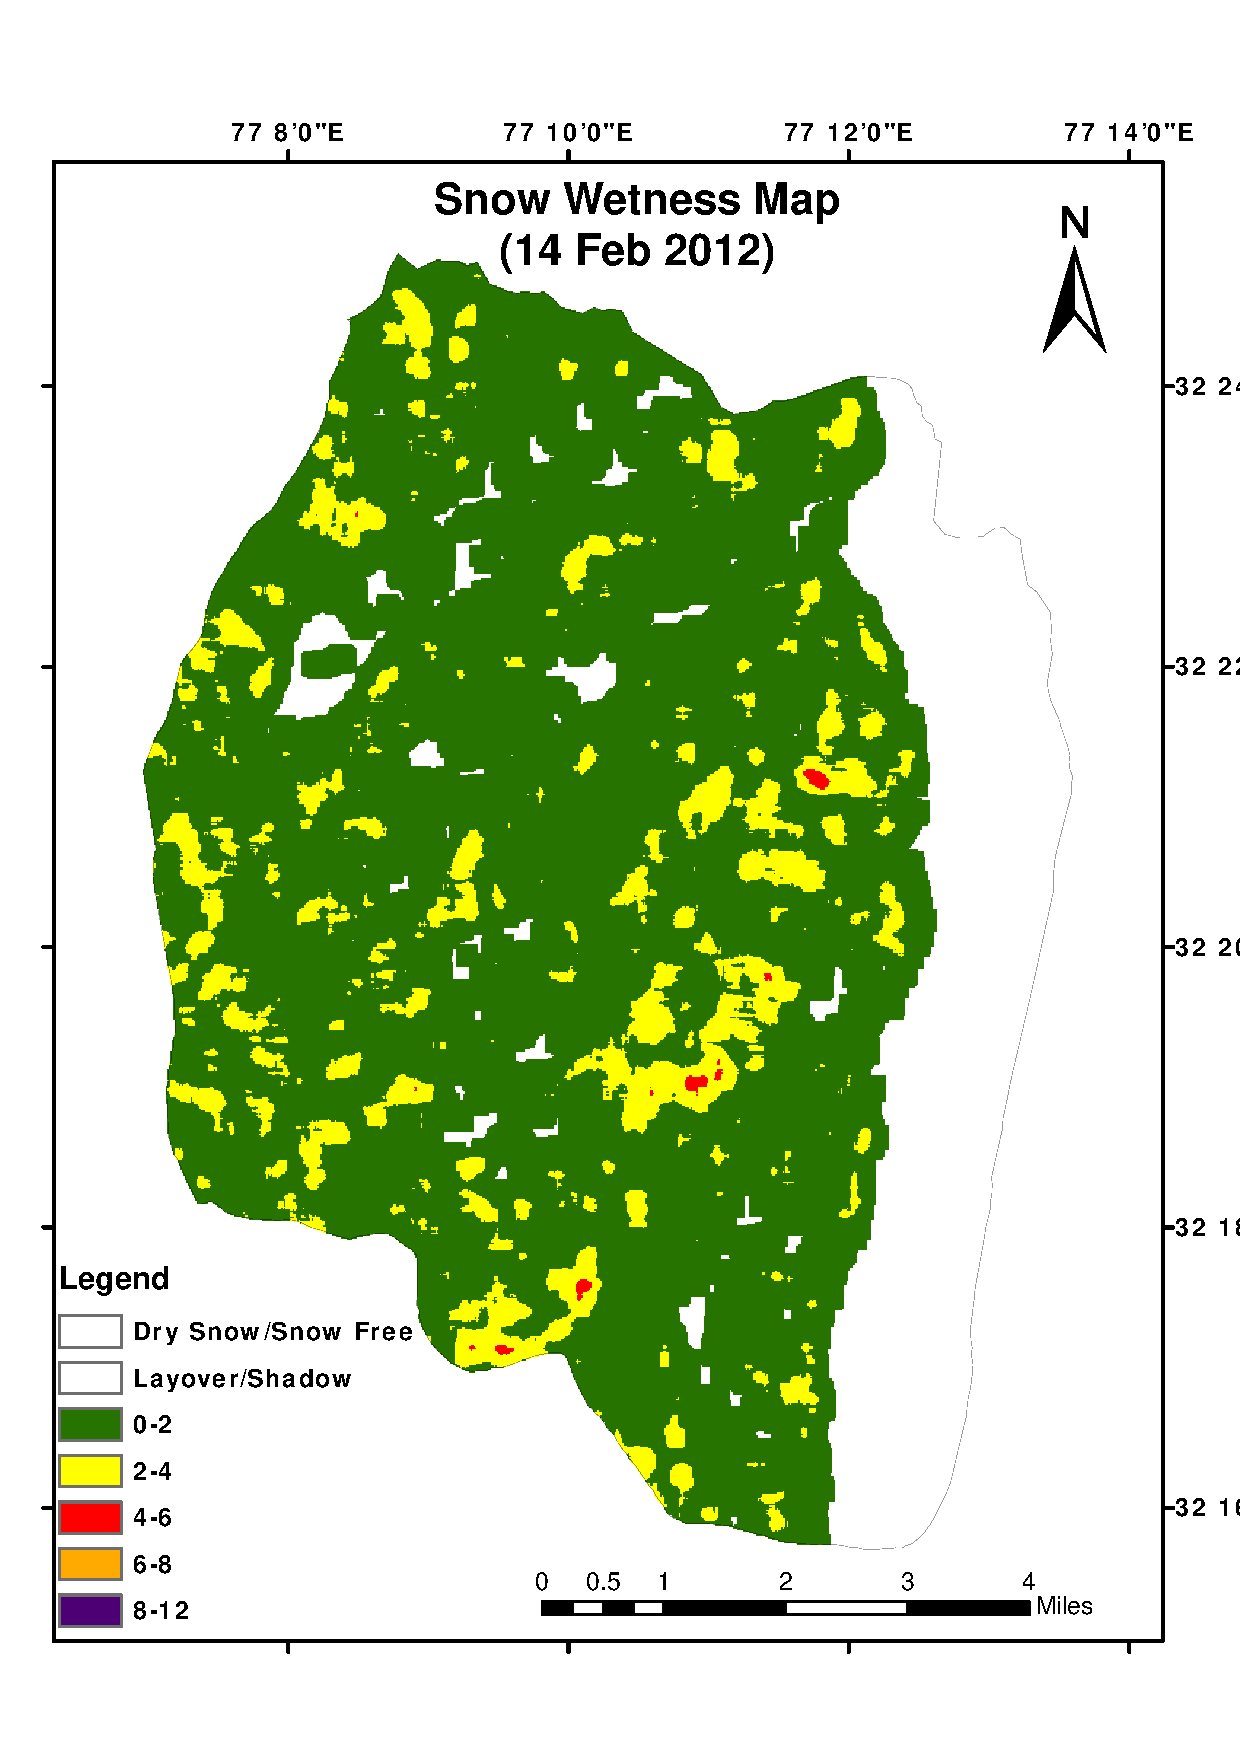
\includegraphics[width=0.45\textwidth]{Figures/14Feb2012}}
	\subfloat[]{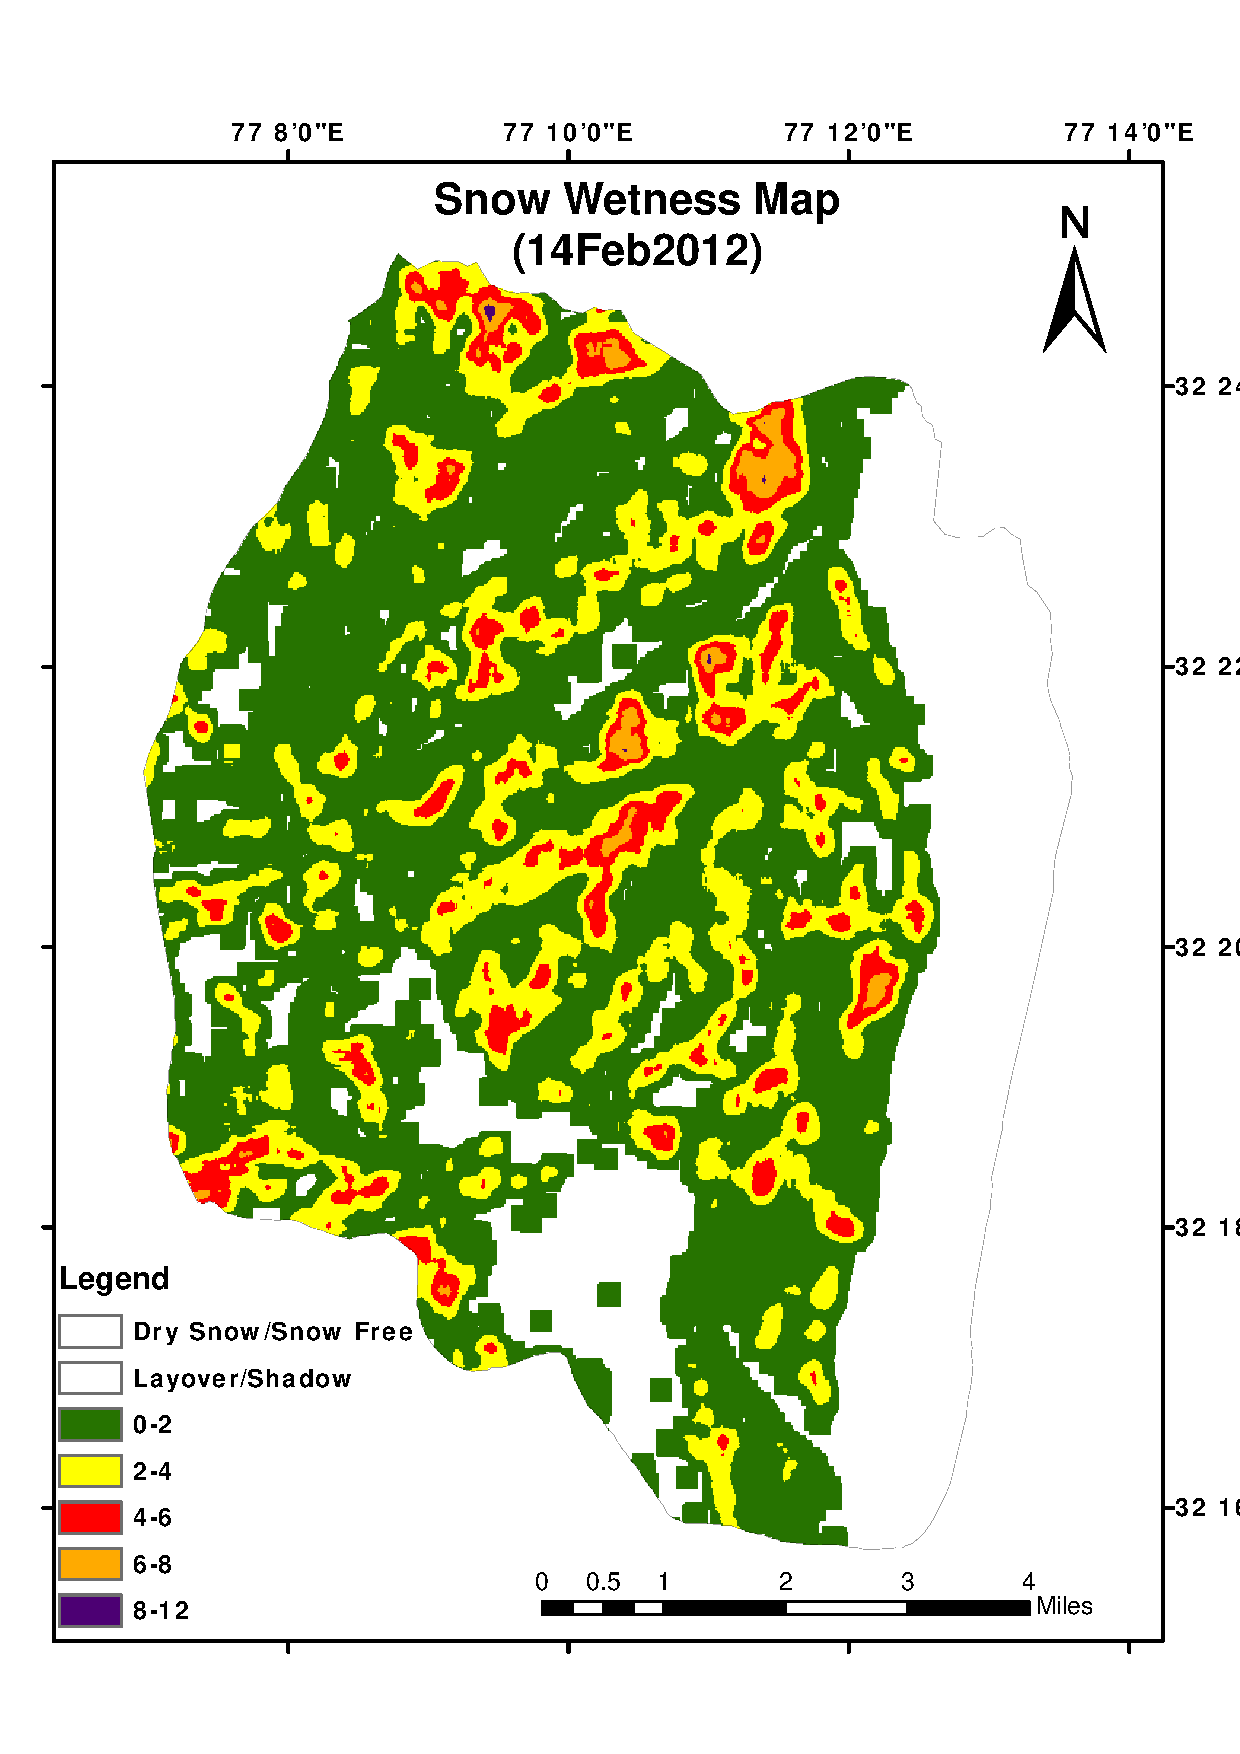
\includegraphics[width=0.45\textwidth]{Figures/14Feb2012_shi}}
	\caption[Comparison of the proposed and Shi~-Dozier snow wetness maps of 14 Feb. 2012 Radarsat-2 data] {Comparison of the snow wetness maps (in $\%$ volume) derived from (a) the proposed and (b) the Shi~-Dozier method. The white blank portion on the right hand side of the map is due to out of data coverage.}
	\label{fig:proposed_shi_dozier_results}
\end{figure}

The snow wetness map for 7 Feb 2012 (Figure~\ref{fig:proposed_results_fullpol1}(a)) data shows that the wetness is in the range of 2--3$\%$ around the Bahang observatory. During this descending pass acquisition, the in-situ measurements were collected around the Bahang observatory and the temperature was recorded around -~2$^\circ$C. The estimated wetness values have a decent concurrence with the field data collected in near-real time with the satellite pass. In the following year, the effective snow wetness was estimated for 6 and 8 Feb 2013 datasets. The snow wetness map derived from the proposed model for the 6 Feb data (Figure~\ref{fig:proposed_results_fullpol1}(b)), shows that the wetness over the Bahang observatory region is around 3--6$\%$ with the maximum temperature of 4$^\circ$C. The wetness is around 1--3$\%$ over the Solang and the Dhundhi observatories where the maximum temperatures were recorded at 1.5$^\circ$C and 1$^\circ$C respectively along with a fresh snowfall on that day. 
\begin{figure}[!thpb]
	\centering
	\subfloat[]{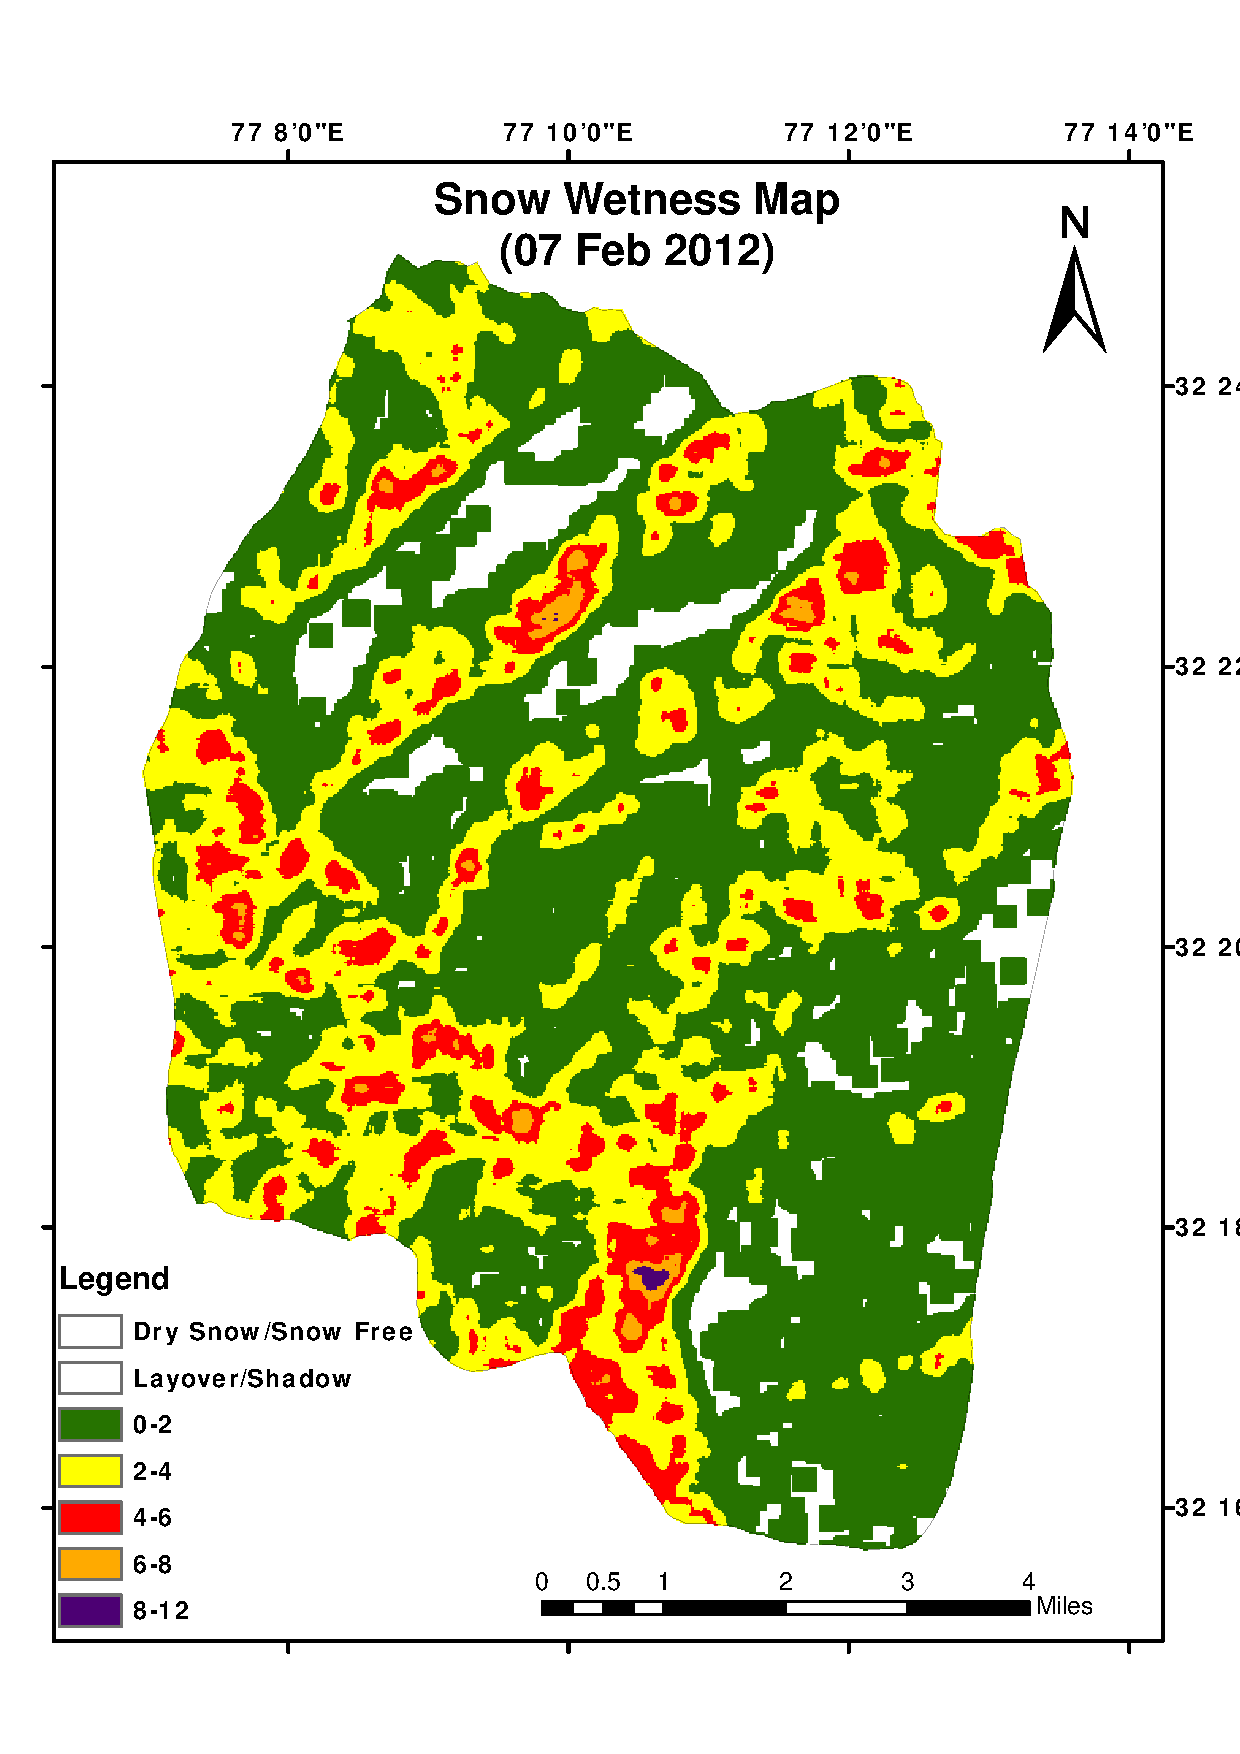
\includegraphics[width=0.45\textwidth]{Figures/07Feb2012}} 
	\subfloat[]{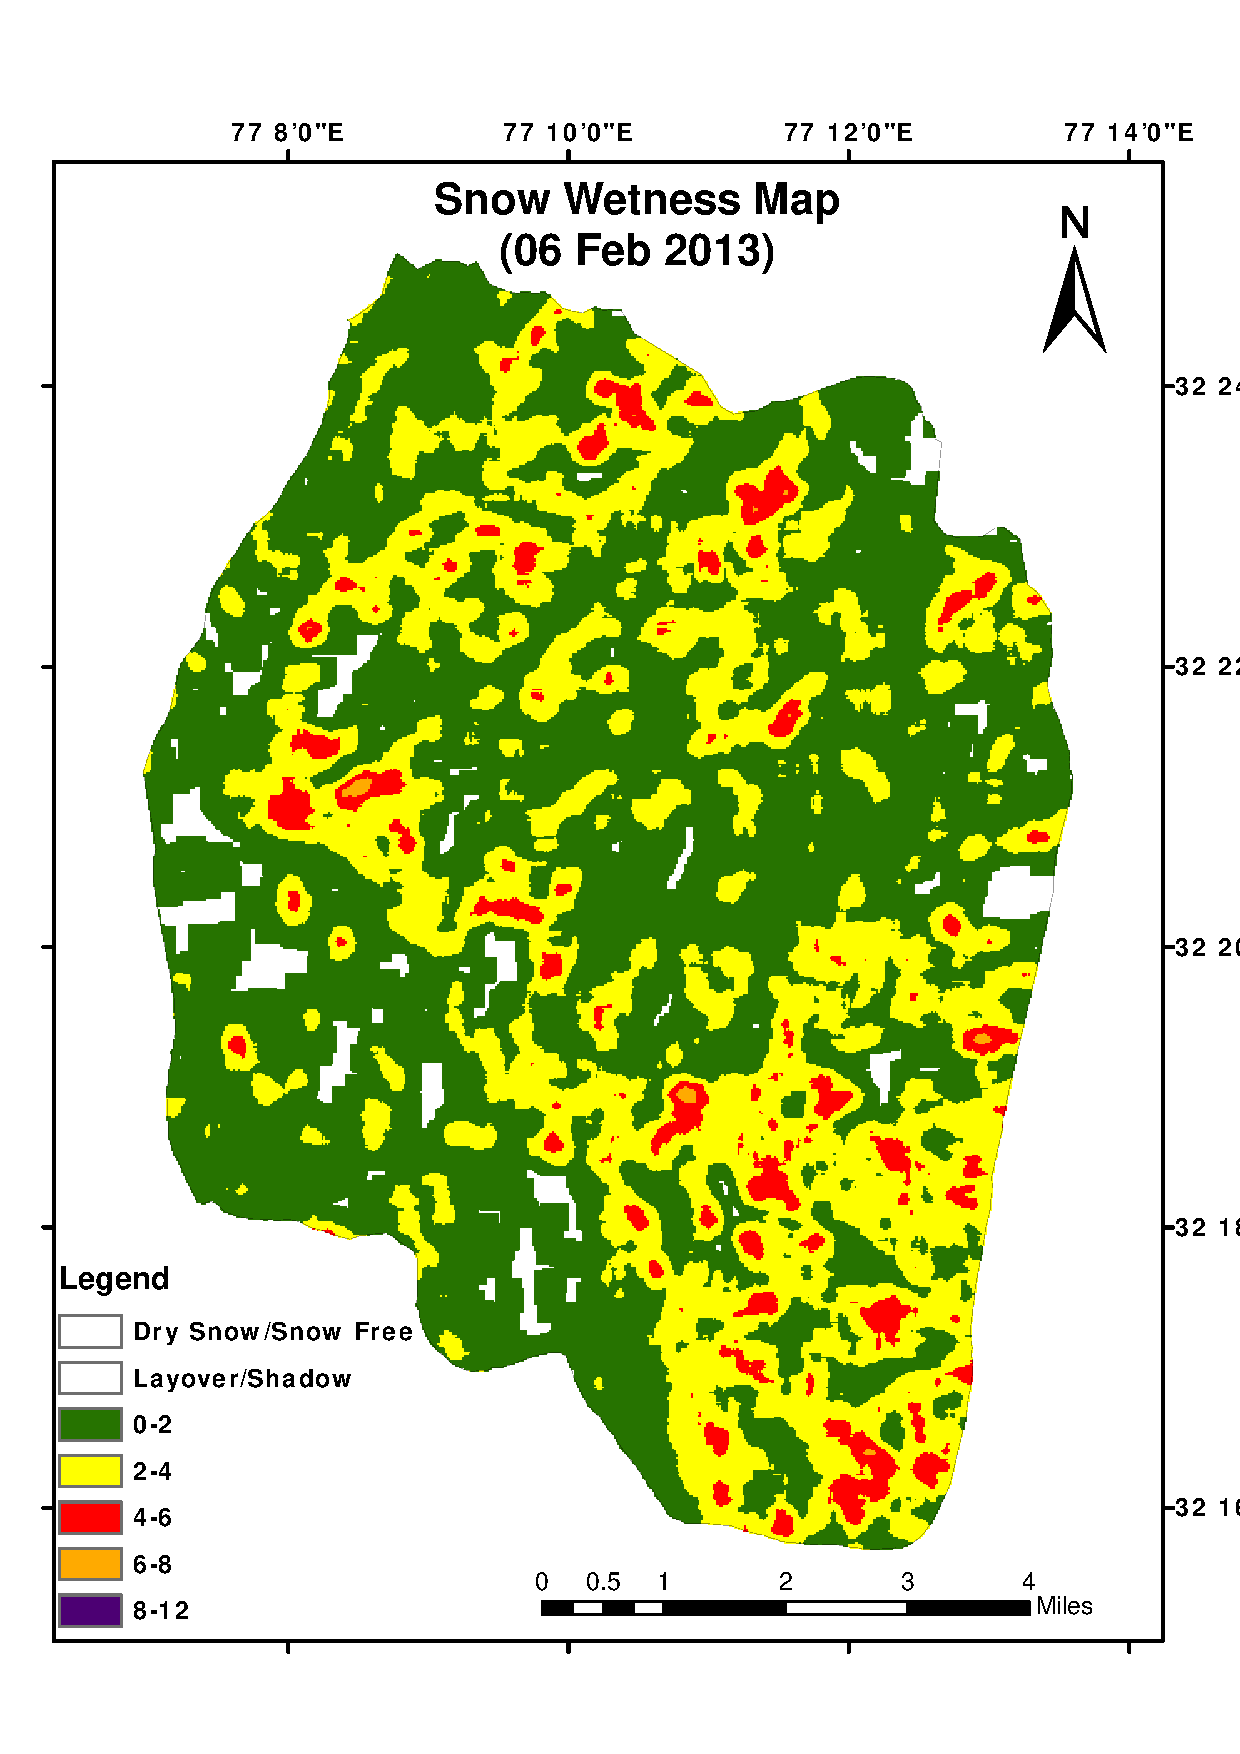
\includegraphics[width=0.45\textwidth]{Figures/06Feb2013}} 
	\caption [Snow wetness maps of 07 Feb. 2012 and 06 Feb. 2013 Radarsat-2 data]{Snow wetness maps (in $\%$ volume) derived from the proposed model.} 
	\label{fig:proposed_results_fullpol1}
\end{figure}

The effective snow wetness map for 18 Feb 2014 is shown in Figure~\ref{fig:proposed_results_fullpol2}(a) which is derived using the weighted average of surface and volume snow wetness maps. It shows that the wetness is in the range of 3--6$\%$ over the study area. The maximum temperature for the day was recorded around 17$^\circ$C, 14$^\circ$C and 8$^\circ$C in the Bahang, Solang and Dhundi observatories, respectively. Due to this high temperature there was a melting of 6 cm, 11 cm and 7 cm of snow within a span of less than 12 hours recorded at the three observatories respectively. This  can be clearly seen in the effective snow wetness map Figure~\ref{fig:proposed_results_fullpol2}(a) which is obtained from the surface (6--9$\%$) and the volume (3--8$\%$) snow wetness maps. This may be due to the melting of snow surface which subsequently percolates into the snowpack, thereby increasing the volume wetness.

\begin{figure}[!thpb]
	\centering
	\subfloat[]{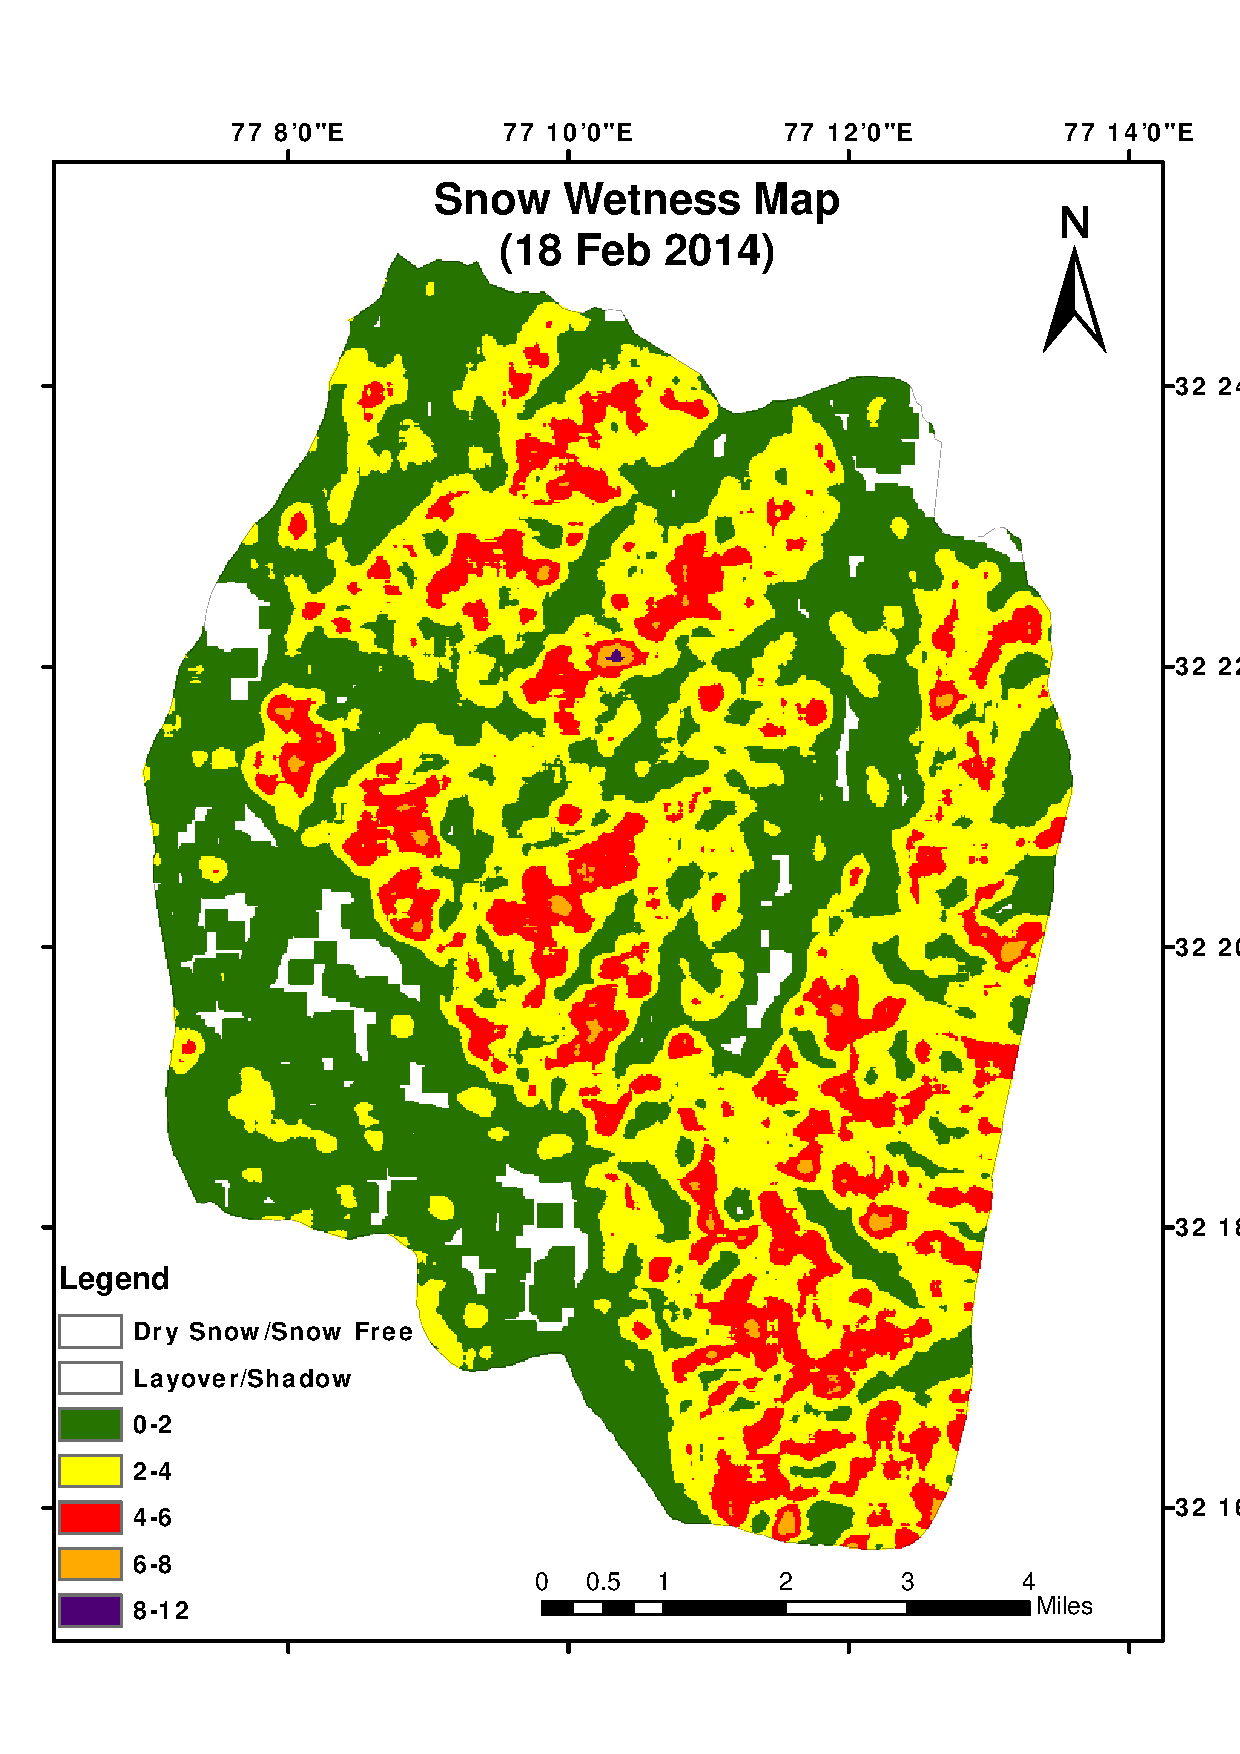
\includegraphics[width=0.45\textwidth]{Figures/18Feb2014}}
	\subfloat[]{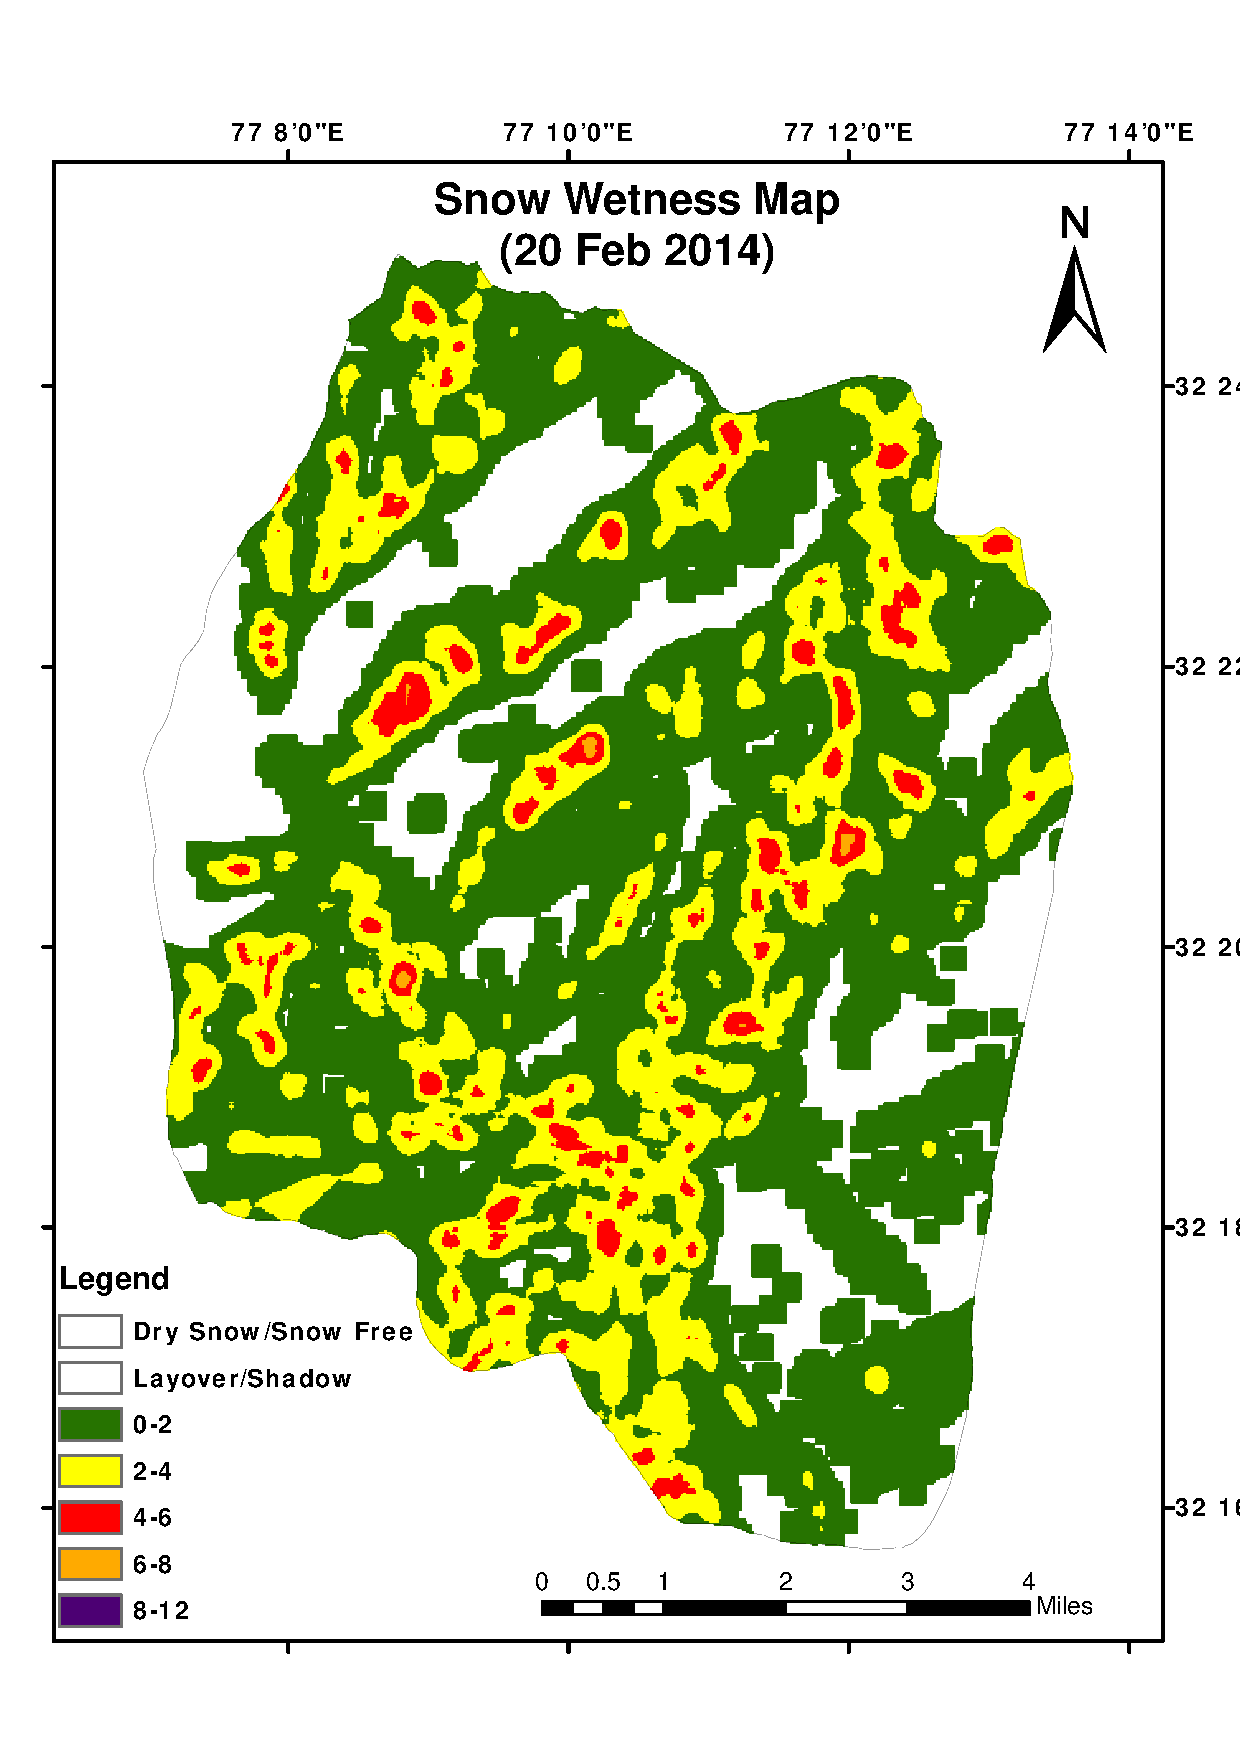
\includegraphics[width=0.45\textwidth]{Figures/20Feb2014}}
	\caption [Snow wetness maps of 18 Feb. 2014 and 20 Feb. 2014 Radarsat-2 data]{Snow wetness maps (in $\%$ volume) derived from the proposed model. RADARSAT-2 Data and Products ©MacDonald, Dettwiler and Associates Ltd. (2014) $–$ All Rights Reserved. RADARSAT is an official trademark of the Canadian Space Agency} 
	\label{fig:proposed_results_fullpol2}
\end{figure}

A total of 40 in-situ measurements were collected in near-real time with the satellite data for three consecutive years to validate the proposed snow wetness estimation algorithm. The snow wetness estimated by the proposed and the Shi-Dozier algorithms along with in-situ measurements are plotted in Figure~\ref{fig:validation_plot_fullpol_SW}(a) and (b) respectively. Particularly for low wetness condition ($<$ 3.5$\%$), the proposed model closely follows the in-situ measurements than the Shi-Dozier method. However, for most of the cases the Shi-Dozier method overestimates the snow wetness. The three in-situ measurements on 7 Feb 2012 over the Dhundi observatory were collected around six hours after the satellite pass. Due to this, the overestimation in the snow wetness is clearly seen in Figure~\ref{fig:validation_plot_fullpol_SW}(a) marked within the black box.
\begin{figure}[!thpb]
	\centering
	\subfloat[]{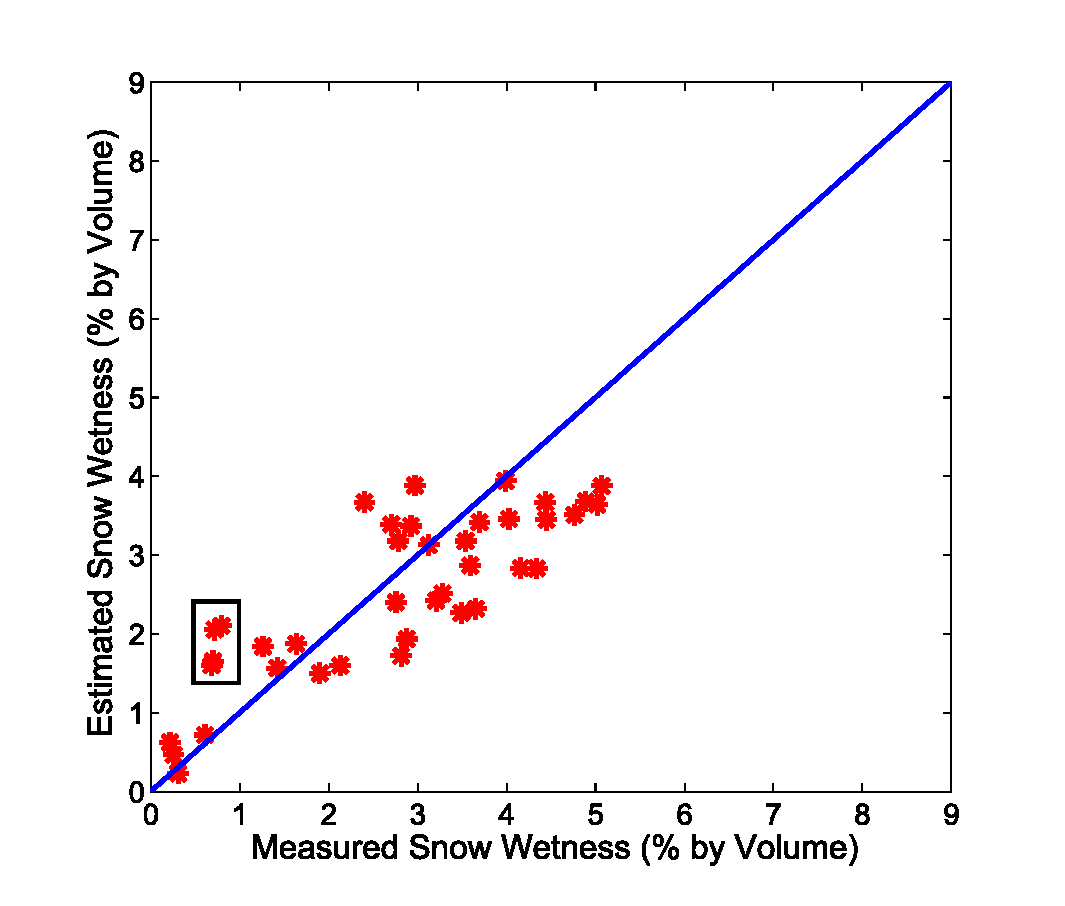
\includegraphics[width=0.45\textwidth]{Figures/validation_plot_proposed}}
	\subfloat[]{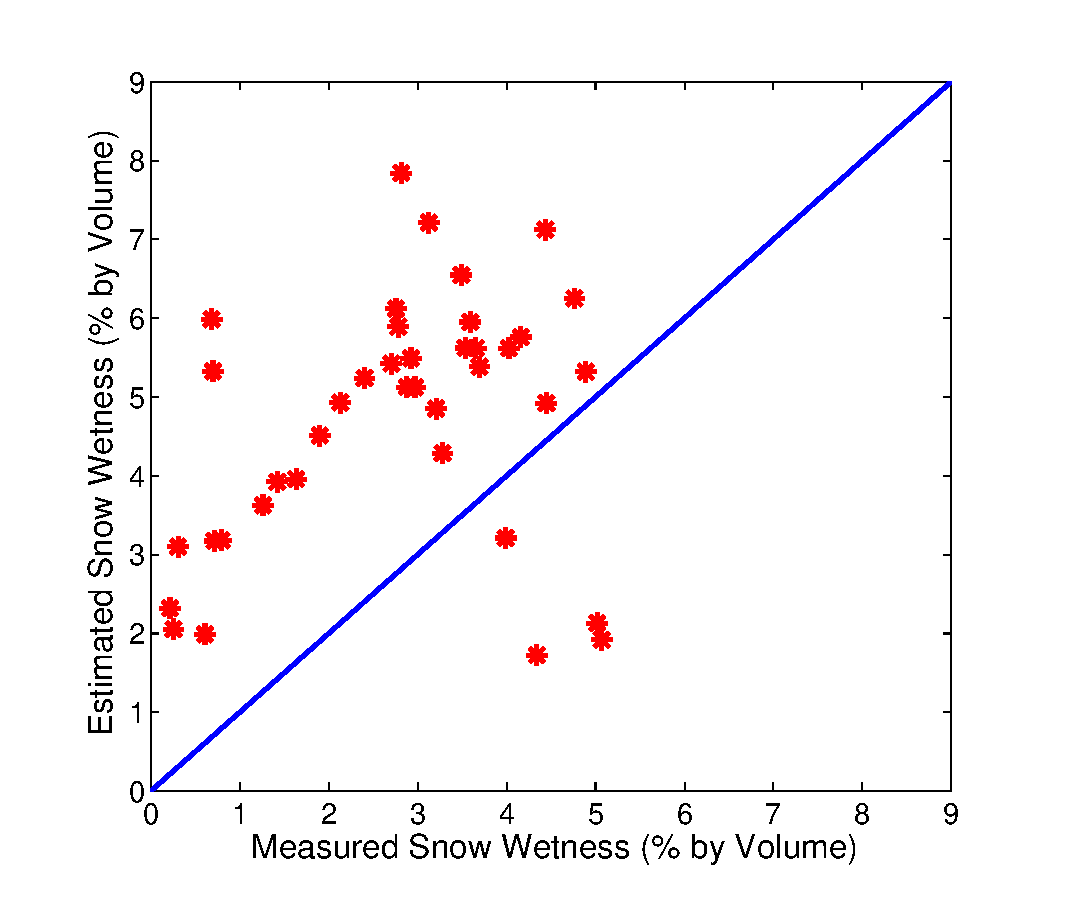
\includegraphics[width=0.45\textwidth]{Figures/validation_plot_shi}}
	\caption [Validation of the snow wetness estimation methods from full polarimetry SAR data]{Comparison of the estimated snow wetness by (a) the newly proposed and (b) the existing Shi~-Dozier methods along with in-situ measurements.} 
	\label{fig:validation_plot_fullpol_SW}
\end{figure}
\FloatBarrier
\section{Snow surface dielectric constant}
\FloatBarrier
\begin{figure*}[!htbp]
	\centering
	\subfloat[]{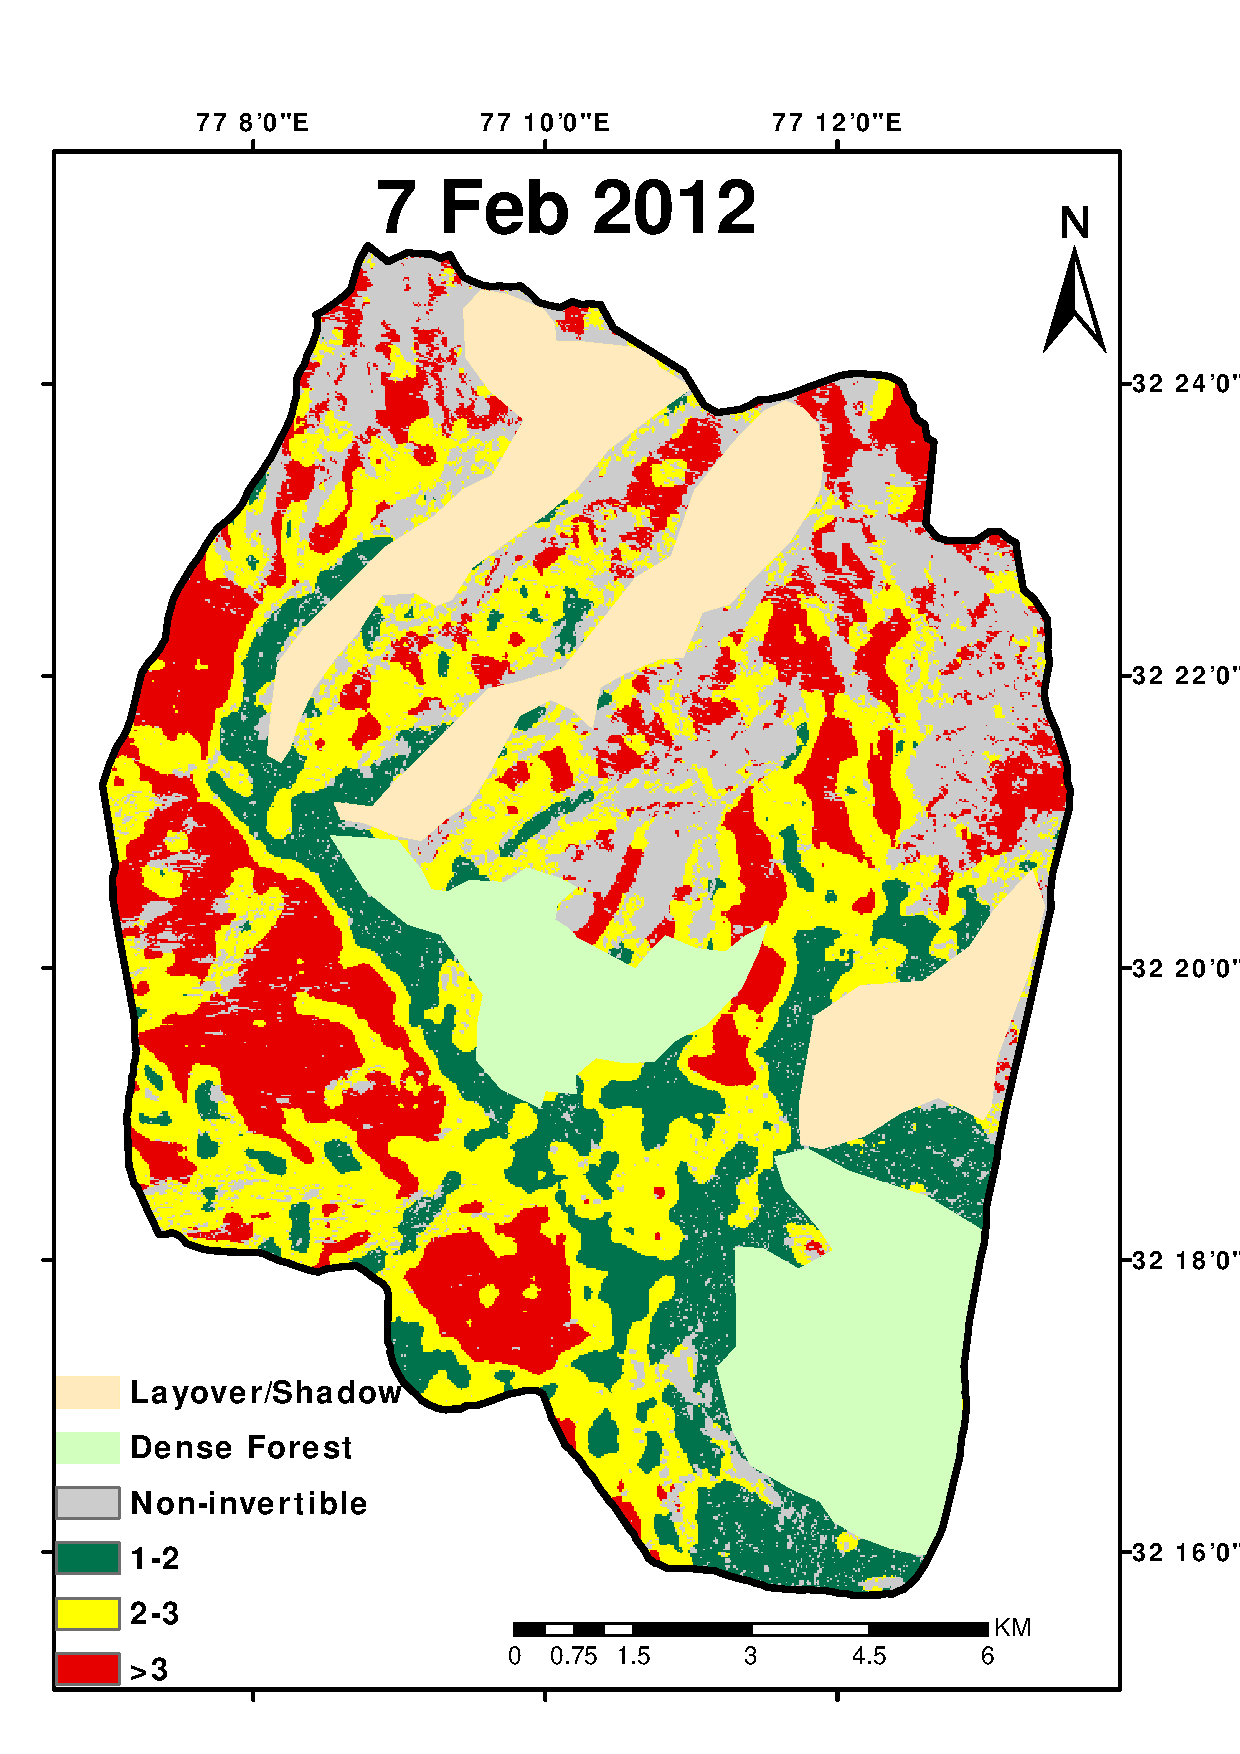
\includegraphics[width=0.45\textwidth]{Figures_SSD/7Feb2012}}
	\subfloat[]{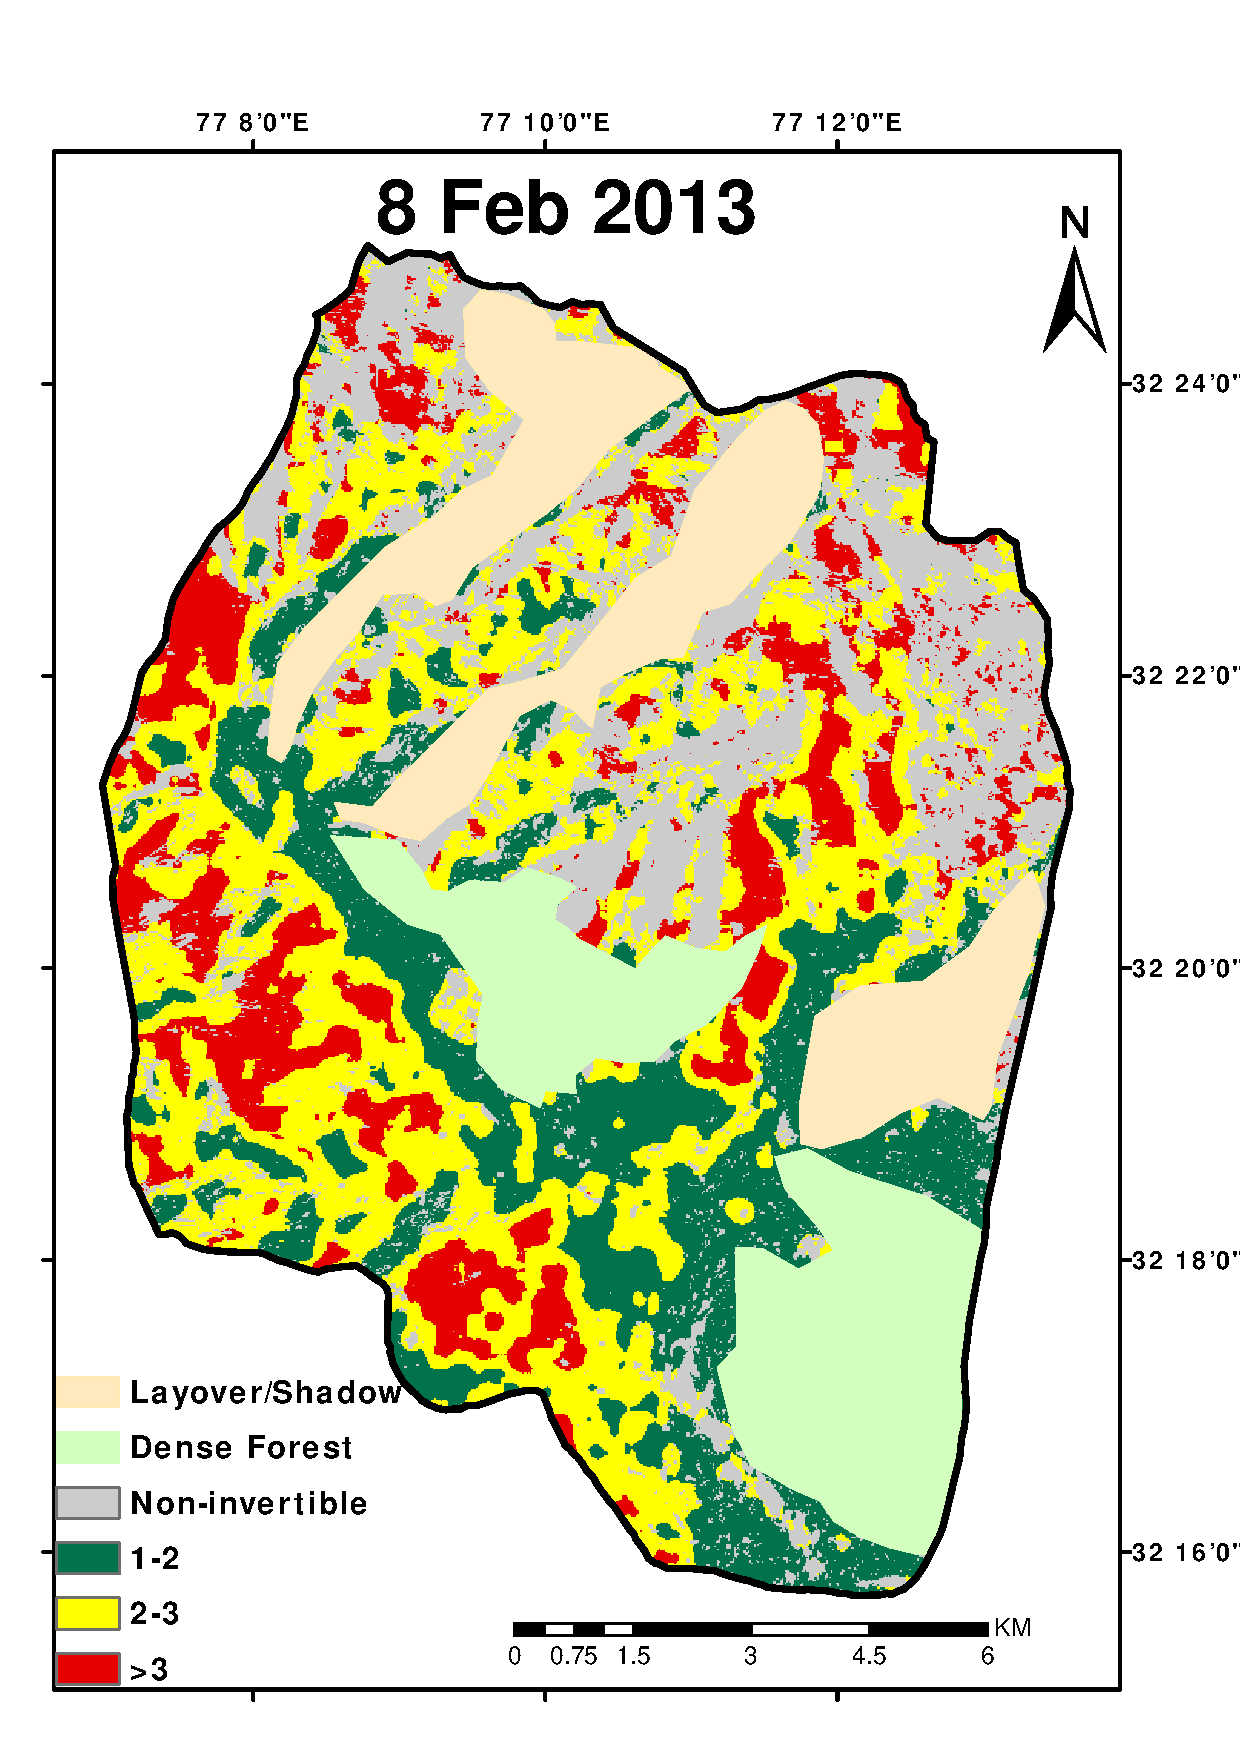
\includegraphics[width=0.45\textwidth]{Figures_SSD/8feb2013}}\\
	\subfloat[]{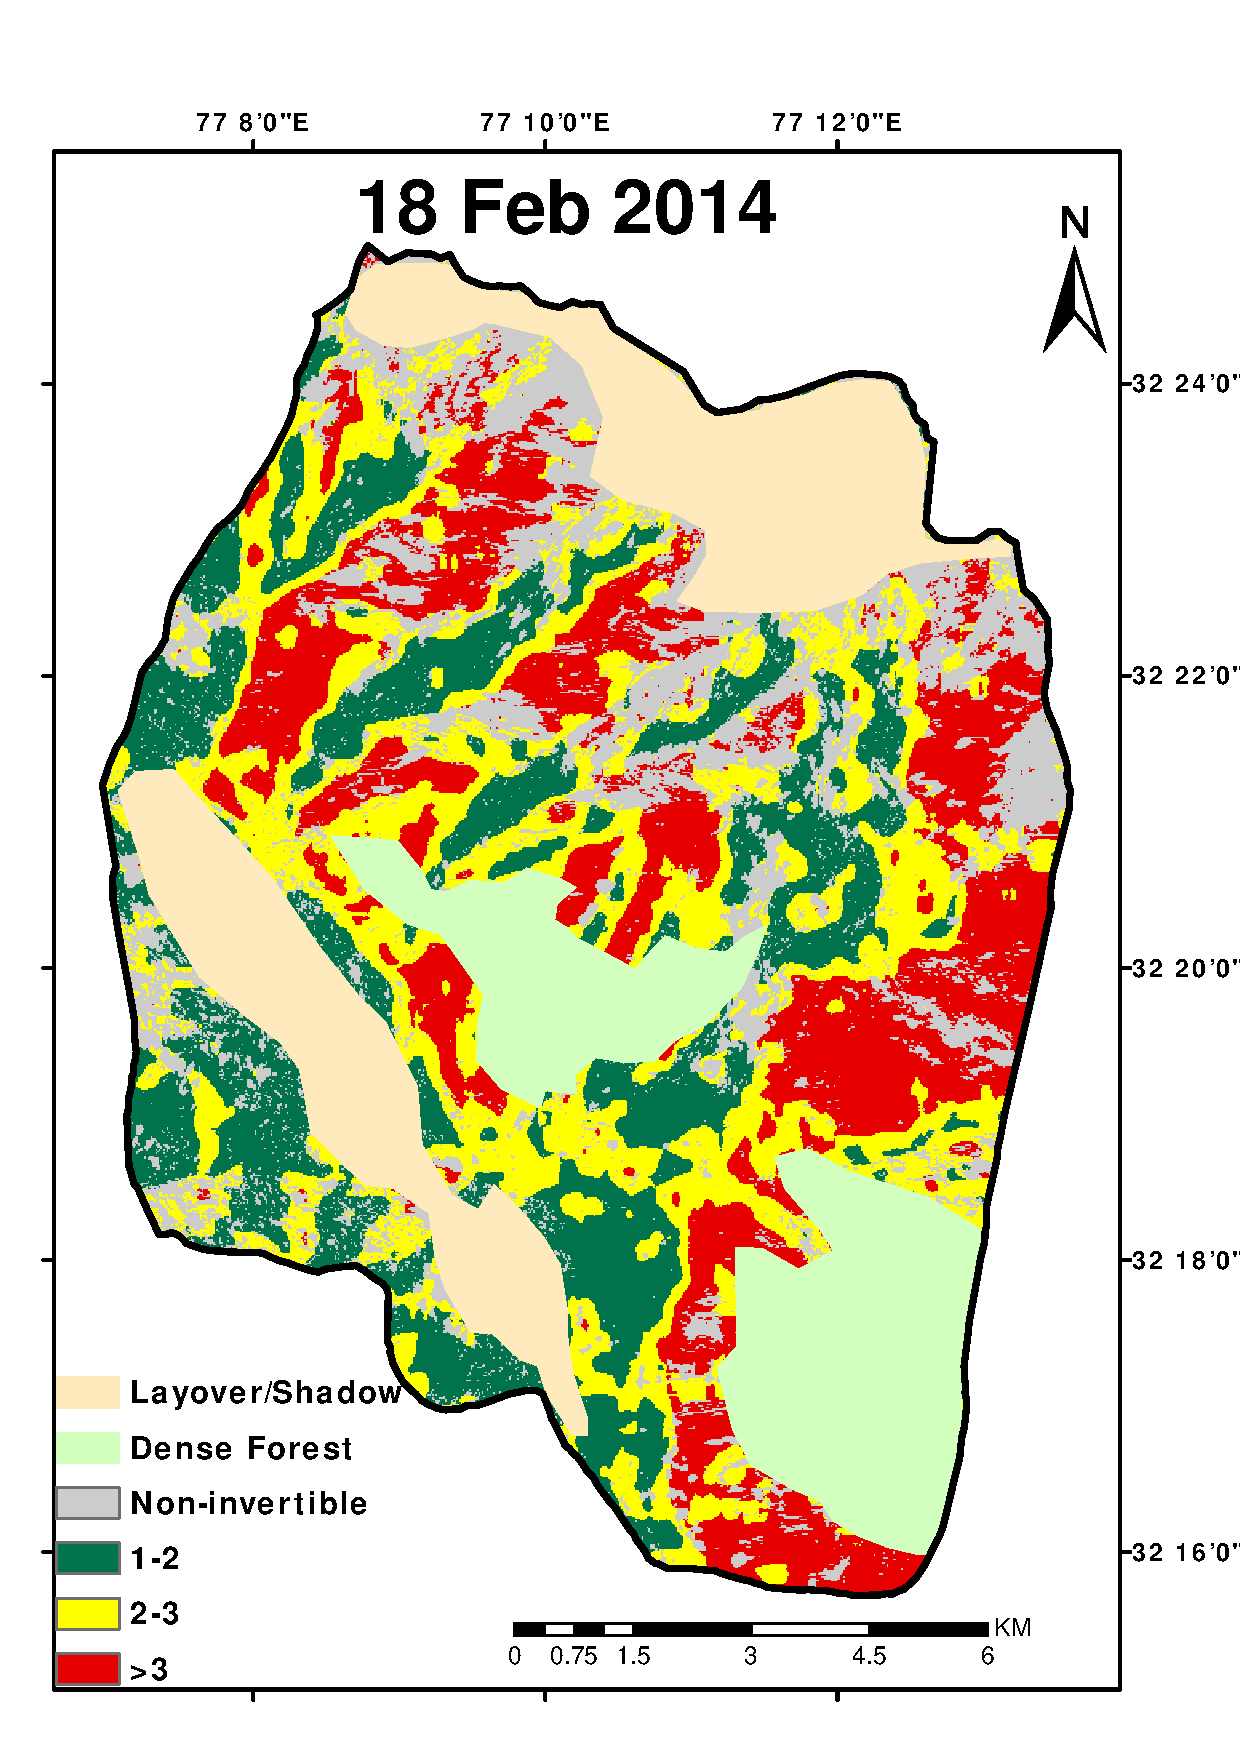
\includegraphics[width=0.45\textwidth]{Figures_SSD/18feb2014}}
	\caption[Snow surface dielectric constant maps]{Temporal snow surface dielectric constant maps estimated over the Manali-Dhundi area for three consecutive winters. (For figure (c): RADARSAT-2 Data and Products ©MacDonald, Dettwiler and Associates Ltd. (2014) $-$ All Rights Reserved. RADARSAT is an official trademark of the Canadian Space Agency)} 
	\label{fig:SSD_results}
\end{figure*}

The proposed algorithm for the estimation of snow surface dielectric constant~(\cref{sec:3.3}) is applied to the fine resolution full-polarimetric Radarsat-2 C-band SAR data acquired over the Manali-Dhundi area in Himachal Pradesh, India~(\cref{sec:4.2.1}). The 3$\times$3 coherency matrix was generated from the single-look complex data. A multi-looking factor of 3 in the range and 4 in the azimuth direction was used to make a pixel square and the Lee-Refined filter was applied to remove the speckle noise. The local incidence angle map is generated while performing the Range Doppler terrain correction using the 30~m SRTM DEM and the Layover/Shadow areas were masked. After these pre-processing, the range and azimuthal pixel spacing of the image was approximately 20~m (19.7~m$\times$20.9~m) respectively. Field campaigns were conducted to collect near-real time in-situ measurements using the snowfork instrument and a hand held GPS with all the three Radarsat-2 data acquisitions for three consecutive winter seasons from 2012 to 2014~(Table~\ref{table:data acquisition}).

%\begin{figure*}[!h]
%	\centering
%	\subfloat[\label{Fig:Snow_surf_diel_7Feb2012}]{\includegraphics[width=0.4\columnwidth]{Figures_SSD/7Feb2012}} \hspace{1mm}
%	\subfloat[\label{Fig:Snow_surf_diel_8Feb2013}]{\includegraphics[width=0.4\columnwidth]{Figures_SSD/8feb2013}} \hspace{1mm}
%	\subfloat[\label{Fig:Snow_surf_diel_18Feb2014}]{\includegraphics[width=0.4\columnwidth]{Figures_SSD/18feb2014}} 
%	\caption{Temporal snow surface dielectric constant maps estimated over the Manali-Dhundi area for three consecutive winters (\protect\subref{Fig:Snow_surf_diel_7Feb2012}, \protect\subref{Fig:Snow_surf_diel_8Feb2013}, \protect\subref{Fig:Snow_surf_diel_18Feb2014}).}
%	\label{fig:results_2}
%\end{figure*}	


%\begin{figure*}[!h]
%	\centering
%	\subfloat[\label{Fig:29Jan2015}]{\includegraphics[width=0.49\columnwidth]{Figures_SSD/SSD_29Jan15}} \hspace{1mm}
%	\subfloat[\label{Fig:22Feb2015}]{\includegraphics[width=0.49\columnwidth]{Figures_SSD/SSD_22Feb15}} 
%	\hspace{1mm}
%	\subfloat[\label{Fig:18Mar2015}]{\includegraphics[width=0.49\columnwidth]{Figures_SSD/SSD_18Mar15}} 
%	\caption{Multi-temporal snow surface dielectric constant maps in a season over the study area}
%	\label{fig:Multi_temporal_SSD}
%\end{figure*}
Using the criteria of $m_{E}^{\mbox{\scriptsize opt}} > 0.5$, it is observed that there is approximately $9-10\%$ increase in the number of invertible pixels compared to the original data $(\langle[{\mathbf{T}}]\rangle)$ for all the data sets used in this study. However, it can be observed that in most areas including higher altitude, $p_{max} > 0.5$ as shown in Figure~\ref{fig:results_1}(b), whereas it is observed that $m_{E}^{\mbox{\scriptsize opt}} < 0.5$ over high altitude regions as shown for 8 Feb. 2013 data in Figure~\ref{fig:results_1}(a). This can be attributed to the fact that: (1). $m_{E}^{\mbox{\scriptsize opt}}$ is obtained in HV basis by minimizing the $T_{33}$ component of the $\langle[\mathbf{T}]\rangle$ matrix unlike $p_{max}$ which is computed over all possible basis $(\chi_{t},\psi_{t})$. (2). Specifically over high altitude regions, $\chi_{t}^{\mbox{\scriptsize opt}} \approx \pm 45^\circ$ (circular polarization) for the corresponding high values of $p_{max}$. This suggests that over these regions $p_{max}$ is obtained for a circular basis (right or left) whereas $m_{E}^{\mbox{\scriptsize opt}}$ is always obtained in the linear HV basis.

Moreover, it can also be observed that even though $p_{max} > 0.5$ over high altitude regions, the basis invariant, $\alpha_{s1}^{B} > 20^\circ$ over those high altitude regions because of the dominant volume scattering mechanisms from the snowpack. Generally in winter the presence of dry and fresh snow cover over high altitude regions ($> 4000$~m) produces snowpack volume scattering. Because of this phenomenon the observed increase in the number of invertible pixels for snow surface dielectric constant using $p_{max} > 0.5$ is just $2\%$ compared to the use of $m_{E}^{\mbox{\scriptsize opt}}$ as shown in Table~\ref{table:SSD_range}. It can also be observed in the scattered plot shown in Figure~\ref{fig:results_1}(d) between the two Dop's ($m_{E}^{\mbox{\scriptsize opt}}$, $p_{max}$) and the dominant scattering type magnitude $\alpha_{s1}$, that the $p_{max}$ values are higher than $m_{E}^{\mbox{\scriptsize opt}}$ in certain ranges. The histogram of the Dop difference $(p_{max} - m_{E}^{\mbox{\scriptsize opt}})$ estimated over the entire study area for the 8 Feb. 2013 data is shown in Figure~\ref{fig:dop_diff}. It can be seen that $p_{max}$ is higher than $m_{E}^{\mbox{\scriptsize opt}}$ by a mean value of just 0.096 with a standard deviation of $\pm 0.1$. Hence, the newly developed AGU optimum Dop ($m_{E}^{\mbox{\scriptsize opt}}$) is used for further analysis in this work.
\begin{figure*}[!htbp]
	\centering
	\includegraphics[width=0.6\columnwidth]{Figures_SSD/dop_diff} 
	\caption [Histogram of the Dop differences]{The histogram of $\Delta\mbox{Dop}=p_{max}-m_{E}^{\mbox{\scriptsize opt}}$ estimated over the study area.}
	\label{fig:dop_diff}
\end{figure*}

\begin{figure*}[!htbp]
	\centering
	\subfloat[]{\includegraphics[width=0.45\columnwidth]{Figures_SSD/DEM_subset}} \hspace{1mm}
	\subfloat[]{\includegraphics[width=0.45\columnwidth]{Figures_SSD/Slop}} \hspace{1mm}
	\subfloat[]{\includegraphics[width=0.65\columnwidth]{Figures_SSD/validation_plot.png}}
	\caption [SRTM 30~m DEM, Slope over the study area and validation plot]{(a). 30 m SRTM DEM and (b). slope map over the study area. (c). Validation Plot }
	\label{fig:DEM,Slope and Validation plot}
\end{figure*}

\begin{figure*}[!htbp]
	\centering
	\subfloat[]{\includegraphics[width=0.45\columnwidth]{Figures_SSD/SSD_29Jan15}} \hspace{1mm}
	\subfloat[]{\includegraphics[width=0.45\columnwidth]{Figures_SSD/SSD_22Feb15}} 
	\hspace{1mm}
	\subfloat[]{\includegraphics[width=0.45\columnwidth]{Figures_SSD/SSD_18Mar15}} 
	\caption[Multi-temporal snow surface dielectric constant maps]{Multi-temporal snow surface dielectric constant maps in a season over the study area. (RADARSAT-2 Data and Products ©MacDonald, Dettwiler and Associates Ltd. (2014) $--$ All Rights Reserved. RADARSAT is an official trademark of the Canadian Space Agency) }
	\label{fig:Multi_temporal_SSD}
\end{figure*}

The estimated snow surface dielectric constant maps for 7 Feb. 2012, 8 Feb. 2013 and 18 Feb. 2014 using the proposed algorithm are shown in Figure~\ref{fig:SSD_results}(a), ~\ref{fig:SSD_results}(b) and ~\ref{fig:SSD_results}(c) respectively. The points A, B and C on the maps indicate the observatory locations at Bahang, Solang and Dhundi which are at an altitude of 2006~m, 2446~m and 2896~m respectively. The percentage of areas covered with different snow surface dielectric constant ranges, for all the three data sets are presented in Table~\ref{table:SSD_range}. It is observed that in all the maps, the snow cover with the surface dielectric constant falling within the range of 2--3 are in most of the areas. Generally in the month of February, the snowfall with considerable temperature variation is observed over the Indian Himalayan region. This condition will initiate the melt-freeze process in the snowpack. 

On 7 Feb. 2012 the descending pass data was acquired around 6.18 AM IST (Indian Standard Time) along with the in-situ measurements collected around the Bahang observatory. The estimated surface dielectric constant values over the Bahang observatory are in the range of 1.5--2 which are closer to the measured values. It can be observed that around 18$\%$ of the area shows the surface dielectric constant values of $>$3. These are mostly over high altitudes along with high slopes (Figure~\ref{fig:DEM,Slope and Validation plot}(a) and Figure~\ref{fig:DEM,Slope and Validation plot}(b)). The Dhundi observatory shows more than 20~cm melting on 6 Feb. 2012. This melting rate might be higher over the slopes than the flat observatory areas. However, during the descending pass acquisition, the observed low temperature ($<-2^\circ$C) might have frozen the melted water over the snow surface within few centimeters. This frozen depth should be lower over the slopes compared to the flat areas. The observed high dielectric constant over the slopes is due to the presence of wet snow layers on the top of the snowpack. These conditions clearly distinguish the low surface dielectric constant over the flat areas and high over the slopes. High wetness and density values over the same slopes have been reported in~\cite{surendar2015snowwetness,surendar2015snowdensity} for the same dataset.

The dielectric constant map for 8 Feb. 2013 (Figure~\ref{fig:SSD_results}(b)) almost follows the same trend as compared to the previous year (7 Feb. 2012). The observed maximum temperature on 7 Feb. 2013 at Bahang, Solang and Dhundi were 11$^\circ$C, 7$^\circ$C and 6$^\circ$C with a melting of around 11~cm, 23~cm and 9~cm, respectively. However, the observed low temperature during the descending pass acquisition at Bahang ($-3^\circ$C), Solang ($-7.5^\circ$C) and Dhundi ($-7^\circ$C) have frozen the snowpack surface similar to the previous year. The snow surface dielectric constant map for the ascending pass data acquired on 18 Feb. 2014 at 6.30 PM IST is shown in Figure~\ref{fig:SSD_results}(c). The different range of values of dielectric constant with snow covered areas for 18 Feb 2014 is shown in Table~\ref{table:SSD_range}. It can be seen from the map (Figure~\ref{fig:SSD_results}(c)) that mostly the areas with high slopes on the eastern side show high dielectric constant range ($>$3). This is because of the direct sun's illumination on the eastern slopes during sunset just before the acquisition. 

Temporal variation of the snow surface dielectric constant map for a 2015 winter season is shown in Figure~\ref{fig:Multi_temporal_SSD}(a)--(c). The snow surface dielectric constant map for 29 Jan. 2015 data is shown in Figure~\ref{fig:Multi_temporal_SSD}(a). It can be observed that over the observatory locations the snow surface dielectric constant values are in the range of 1--2 and which are increasing over the low altitude slopes. This may be because of no fresh snowfall on 28 Jan. 2015 and the maximum temperature observed was 3$^\circ$C, 9.5$^\circ$C and 11$^\circ$C at Dhundhi, Solang and Bahang stations, which melts the snow surface considerably. But during the acquisition observed minimum temperature (-7$^\circ$C, -3.5$^\circ$C and -1.5$^\circ$C at Dhundhi Solang and Bahang observatories respectively) might have frozen the snow surface in few cm over flat observatory locations and which are low over the slope areas. But over high altitude regions the pixels are mostly non-invertible. This may be because of the fresh snowfall which produces dominant volume scattering mechanism.The total percentage of the invertible pixels for snow surface dielectric constant was around 30$\%$ for this data.  
%In the high altitude  over the observatory locations. The minimum temperature on that day were . Fresh snow fall was observed on Solang and Dhundhi observatories but no fresh snow fall on 28 Jan 2015. The maximum temperature observed was 3$^\circ$C, 9.5$^\circ$C and 11$^\circ$C at Dhundhi, Solang and Bahang stations, which melts the snow surface (the standing snow at all the three observatories were 158~cm, 90~cm and 12~cm respectively) But the minimum temperature frozen the melting water in few cm in flat observatory locations and which are low over the slop areas. 
\begin{table}[!htbp]
	\caption[Comparison of invertible pixels by both the optimization techniques]{Comparison of the percentage of area utilized for the snow surface dielectric constant inversion using the criteria for $(m_{E}^{\mbox{\scriptsize opt}})$ and $(p_{max})$. }
	\begin{center}
		\begin{tabular}{|c|c|c||c|c||c|c|} \hline
			Dielectric Range & \multicolumn{6}{c|}{Area ($\%$)} \\
			\cline{2-7}
			& \multicolumn{2}{c||}{7 Feb. 2012} & \multicolumn{2}{c||}{8 Feb. 2013} & \multicolumn{2}{c|}{18 Feb. 2014}\\
			\cline{2-7}
			& $m_{E}^{\mbox{\scriptsize opt}}$ & $ p_{max}$ & $m_{E}^{\mbox{\scriptsize opt}}$ & $p_{max}$ & $m_{E}^{\mbox{\scriptsize opt}}$ & $p_{max}$ \\ \hline
			1-2 &	13.77 & 13.91 & 17.03 & 17.61 & 17.54 & 18.21 \\ \hline
			2-3 &	24.44 & 25.30 & 25.26 & 26.37 & 19.93 & 21.04 \\ \hline
			$>$3&   18.31 & 18.90 & 11.91 & 12.64 & 17.53 & 17.86 \\ \hline
			\bf Total&  \bf 56.52 & \bf 58.11 & \bf 54.2 & \bf 56.52 & \bf 55.00 & \bf 57.11 \\ \hline \hline
			Dense forest cover & 12.59 &	12.59 &	12.59 & 12.59 & 12.59 & 12.59 \\ \hline
			Layover/Shadow & 12.67 & 12.67 & 12.67 & 12.67 & 15.42 & 15.42 \\ \hline
		\end{tabular}
	\end{center}
	\label{table:SSD_range}
\end{table}

The snow surface dielectric constant map for 22 Feb. 2015 is shown in Figure~\ref{fig:Multi_temporal_SSD}(b). There was no snowfall observed on 21 $\&$ 22 Feb. 2015 over the study area. As per the temperature fluctuation within a day snow started to melt and freeze. During the acquisition snow surface got frozen because of the low temperature. Since, there was no recent snowfall the top snow surface layers are wet which produces dominant surface scattering. So that, the total percentage of the invertible pixels for snow surface dielectric constant was around 40$\%$ for this data. For the data of 18 Mar. 2015, the snow surface dielectric constant (Figure~\ref{fig:Multi_temporal_SSD}(c)) was inverted for around 35 $\%$ of pixels which was lower than the 22 Feb 2015 data. This may be because of the observed fresh snowfall of 5~cm and 25~cm over Solang and Dhundhi regions on 17 March 2015.  Most of the higher altitude pixels are not invertible because of this fresh snowfall.

A total of 20 in-situ measurements were collected in near real time with the satellite data for the three consecutive years to validate the proposed snow surface dielectric constant estimation algorithm. The snow surface dielectric constant estimated by the proposed algorithm along with in situ measurements is plotted in Figure~\ref{fig:DEM,Slope and Validation plot}(c). The dielectric constant of top 5~cm of the snowpack is considered as the snow surface dielectric constant for validation of the proposed method. The correlation coefficient between the measured and the estimated snow surface dielectric constant is 0.95 at 95$\%$ confidence interval with a root mean square error (RMSE) of 0.20. The snow surface dielectric constant estimated from G4U based generalized surface parameter (~\cref{sec:3.2}) is compared with this proposed new method and validated using the in-situ measurements~(\ref{fig:comparision_of_SSD}). The correlation coefficient between the measured and the G4U based snow surface dielectric constant is 0.92 at 95$\%$ confidence interval with a root mean square error (RMSE) of 0.22.

\begin{figure*}[!htbp]
	\centering
	\includegraphics[width=0.6\columnwidth]{Figures_SSD/Comparision_plot} 
	\caption [Comparision of SSD]{Comparision of SSD estimated from $\alpha_{s1}$ and the G4U based method with the in-situ measurements }
	\label{fig:comparision_of_SSD}
\end{figure*}



%\begin{figure*}[!h]
%	\centering
%	\subfloat[\label{Fig:DEM}]{\includegraphics[width=0.4\columnwidth]{Figures_SSD/DEM_subset}} \hspace{1mm}
%	\subfloat[\label{Fig:Slop}]{\includegraphics[width=0.4\columnwidth]{Figures_SSD/Slop}} \hspace{1mm}
%	\subfloat[\label{Fig:Validation_plot}]{\includegraphics[width=0.65\columnwidth]{Figures_SSD/validation_plot.png}}
%	\caption{\protect\subref{Fig:DEM}. 30 m SRTM DEM and \protect\subref{Fig:Slop} slope map over the study area. \protect\subref{Fig:Validation_plot} Validation Plot }
%	\label{fig:results_3}
%\end{figure*}
\FloatBarrier
\section{Snow density}
\label{S:4}

In this section, the algorithm proposed in~\cref{sec:3.4} for the estimation of snow density from full polarimetric SAR data is analyzed using Radarsat-2 C-band SAR data. The results are analyzed over the study area explained in~\cref{sec:4.2.1}. The snow density estimated by the proposed method for 7 Feb. 2012 data is given in Figure~\ref{fig:proposed_results}(a). The range of 0.2--0.35~gcm$^{-3}$ density value occupies a maximum extent of about 46$\%$ of total study area (Table.~\ref{table:snow_density_range}). The observed density range in the map is possibly due to the increased grain size by the snowpack compaction. This is understood by studying the meteorological record at Dhundhi observatory (Figure~\ref{fig:multi_temp_plots}(a),(b)). From 6 to 7 Feb. 2012, the recorded temperature increased from 2$^\circ$C to 5$^\circ$C and wind speed of 2--4 km/hr, causing snow metamorphism. Also during this period the snowpack depth reduced by 33~cm as per the observatory data. Both the temperature and the wind speed together might have caused the reduction of snow depth and the compaction of the snowpack (~\citep{MET40}). In the map Figure~\ref{fig:proposed_results}(a), around 25$\%$ of the study area shows dense forest and geometric distortions (Table.~\ref{table:snow_density_range}). All the Radarast-2 descending pass data over this region possibly shows this distortions.

\begin{figure*}[!htbp]
	\centering
	\subfloat[]{\includegraphics[width=0.45\textwidth]{Figures_sd/7Feb2012}}
	\subfloat[]{\includegraphics[width=0.45\textwidth]{Figures_sd/8Feb2013}} \\
	\subfloat[]{\includegraphics[width=0.45\textwidth]{Figures_sd/18Feb2014}}
	\caption [Snow density mps from Radarsat-2 data]{Snow density maps derived from the proposed methodology. (For figure (c): RADARSAT-2 Data and Products ©MacDonald, Dettwiler and Associates Ltd. (2014) $-$ All Rights Reserved. RADARSAT is an official trademark of the Canadian Space Agency)}
	\label{fig:proposed_results}
\end{figure*}

\begin{table}[!htbp]
	\caption{Percentage of area with snow density range}
	\begin{center}
		\begin{tabular}{|c|c|c|c|} \hline
			Snow Density Range (gcm$^{-3}$) & \multicolumn{3}{c|}{Area $\%$} \\
			\cline{2-4}
			& 7 Feb. 2012 & 8 Feb. 2013 & 18 Feb. 2014 \\ \hline
			0.0--0.05 &	1.38 &	2.86 &	1.84 \\ \hline
			0.05--0.1 &	0.73 &	4.15 &	0.98 \\ \hline
			0.1--0.15 &	3.10 &	4.75 &	3.65 \\ \hline
			0.15--0.2 &	5.79 &	5.70 &	5.07  \\ \hline
			0.2--0.25 &	14.00 &	7.17 &	9.03 \\ \hline
			0.25--0.3 &	20.28 &	7.20 &	14.24 \\ \hline
			0.3--0.35 &	11.80 &	3.78 &	11.01 \\ \hline
			0.35--0.4 &	4.02 &	0.92 &	5.10 \\ \hline
			0.4--0.45 &	1.82 &	0.15 &	2.87 \\ \hline
			0.45--0.5 &	0.37 &	0.01 &	1.13 \\ \hline
			\hline		
			Dense forest cover &	12.59 &	12.59 &	12.59 \\ \hline
			Layover/Shadow &	12.67 &	12.67 &	15.42 \\ \hline
			Snow free/Wet snow &	11.42 &	38.06 &	17.06 \\ \hline
		\end{tabular}
	\end{center}
	\label{table:snow_density_range}
\end{table}


During the same period in the following year (8 Feb. 2013), the density was estimated in the range of 0.2--0.3~gcm$^{-3}$ as shown in Figure~\ref{fig:proposed_results}(b). This range of density values covers around 15$\%$ of the entire study area as shown in Table.~\ref{table:snow_density_range}. However, snow free/wet snow regions in the snow density map were around 38$\%$ as seen in Table.~\ref{table:snow_density_range}. This might be because of the maximum temperature recorded on 7 Feb. 2013. The observed temperatures at the Bahang, Solang and Dhundhi observatories on 7 Feb. 2013 were 11$^\circ$C, 7$^\circ$C and 6$^\circ$C (Figure~\ref{fig:multi_temp_plots}(c)), respectively which were higher than 2012. However, it can be observed that the snow density values are lower than the previous year (7 Feb. 2012). This may be because of the fresh snowfall on 6 Feb. 2013. Even though high temperature was observed on 7 Feb. 2013, the snowpack might not have compacted firmly during the acquisition on 8 Feb. 2013 as compared to the multiple melt-freeze condition in 2012. 

The estimated snow density map and the observatory measurements for the 18 Feb. 2014 data (Figure~\ref{fig:proposed_results}(c)), shows a similar trend as that of 7 Feb. 2012. Unlike the 7 and 8 Feb, the 18 Feb. 2014 data was acquired in an ascending pass. It can be seen in Table.~\ref{table:snow_density_range} that 34$\%$ of the area was covered with the snow density values in the range of 0.2--0.35~gcm$^{-3}$. There was no fresh snowfall recorded for a week prior to the acquisition on 18 Feb. 2014. Moreover, a large variation can also be observed between the maximum and the minimum temperatures on 18 Feb. 2014 (Figure~\ref{fig:multi_temp_plots}(d)). So the old snowpack has undergone multiple melt-refreeze process, which has increased the snowpack grain size and consequently, the snow density. 

\begin{figure*}[!htbp]
	\centering
	\subfloat[]{\includegraphics[width=0.49\textwidth]{Figures_sd/Temp_variability_jan_2015}}
	\subfloat[]{\includegraphics[width=0.49\textwidth]{Figures_sd/Temp_variability_feb_2015}} \\
	\subfloat[]{\includegraphics[width=0.49\textwidth]{Figures_sd/Temp_variability_mar_20151}} 
	\caption [Temperature variation plots]{Temporal variation of average local temperature over the study area in (a) Jan 2015; (b) Feb 2015; (c) March 2015 (the data were taken from the site:http://www.accuweather.com as on 17 April 2015)}
	\label{fig:temp_plots_2015}
\end{figure*}

\begin{figure*}[!htbp]
	\centering
	\subfloat[]{\includegraphics[width=0.49\textwidth]{Figures_sd/Temp_variability_2012}} \hspace{0.1cm}
	\subfloat[]{\includegraphics[width=0.49\textwidth]{Figures_sd/windspeed_variability_2012}} \\
	\subfloat[]{\includegraphics[width=0.49\textwidth]{Figures_sd/Temp_variability_observatories_2013}}\hspace{0.1cm} 
	\subfloat[]{\includegraphics[width=0.49\textwidth]{Figures_sd/Temp_variability_observatories_2014}} 	
	\caption[Temperature and windspeed variation over Dhundhi observatory]{(a) Temporal variation of temperatures over Dhundhi in Feb. 2012; (b) Temporal variation of wind speed over Dhundhi in Feb. 2012; (c)-(d) Temporal variation of minimum and maximum temperatures over all the three observatories in Feb 2013 and 2014 respectively}
	\label{fig:multi_temp_plots}
\end{figure*}

The Radarsat-2 data acquired with the same geometry on 29 Jan, 22 Feb and 18 Mar. 2015 was used to analyze the snow density changes within a season. The snow density map of 29 Jan 2015 (Figure~\ref{fig:multi_temp_density}(a)) indicates that the study area was completely covered with fresh snow. The estimated snow density values are less than 0.1 gcm$^{-3}$ in most of the areas as shown in Figure~\ref{fig:multi_temp_density}(a). Generally, by the end of January, high amount of snow precipitation occurs in the Indian Himalaya. This is reflected in the map with low snow density values. The local averaged temperature plot (Figure~\ref{fig:temp_plots_2015}(a)), shows that the temperature drops to 4$^\circ$C during the acquisition day. This is the lowest temperature recorded during that particular week which may be because of fresh snowfall on that day. 

\begin{figure*}[!htbp]
	\centering
	\includegraphics[width=0.9\textwidth]{Figures_sd/temporal_variability_SD}
	\caption[Multi temporal snow density maps] {Temporal variation of snow density in a season. (RADARSAT-2 Data and Products ©MacDonald, Dettwiler and Associates Ltd. (2014) $--$ All Rights Reserved. RADARSAT is an official trademark of the Canadian Space Agency)}
	\label{fig:multi_temp_density}
\end{figure*}

The estimated snow density values were more than 0.2 gcm$^{-3}$ for most of the study area on 22 Feb. 2015, as shown in Figure~\ref{fig:multi_temp_density}(b). Normally in February, snowfall occurs and large variations between the minimum and the maximum temperatures were observed within a day. Hence, considerable melting and refreezing occurs in the snowpack which increases the snow density. As observed in Figure~\ref{fig:temp_plots_2015}(b), the averaged local temperature before the acquisition day was recorded at 12$^\circ$C. So, the snow surface melt might have refrozen during the descending pass acquisition (6.14 AM local IST). 

Snow density map of 18 Mar. 2015 shows that $>$ 0.3 gcm$^{-3}$ of snow density values are observed in most of the study area which is high as compared to the snow density map of February. Normally in March, the snowfall stops and the snowpack starts to melt. The white areas in this map (non-invertible pixels) possibly represents wet snow. This can be attributed to high temperature (Figure~\ref{fig:temp_plots_2015}(c)) which may have melted the snow surface so it causes the absence of snowpack volume scattering.

\begin{figure*}[!htbp]
	\centering
	\includegraphics[width=0.5\textwidth]{Figures_sd/snow_density_validation}
	\caption [validation plot of snow density algorithm]{Comparison of the snow densities estimated by the proposed methodology and in-situ measurements.}
	\label{fig:validation_plot}
\end{figure*} 

A total of 23 near-real time in-situ measurements were collected with the satellite data for three consecutive years to validate the proposed snow density estimation algorithm. The snow densities estimated by the proposed methodology and measured in the field are plotted in Figure~\ref{fig:validation_plot}. The mean absolute error (MAE) of  the proposed method is 0.027~gcm$^{-3}$ and the root mean square error (RMSE) is 0.032~gcm$^{-3}$. 




\chapter{Summary and Conclusions}

In this thesis, the utilization of complete polarimetric SAR information for the estimation of snowpack parameters is described. Snow parameters in mountain areas are particularly sensitive to changes in environmental conditions. Timely gathering information about snow parameters and their temporal and spatial variability represents a significant contribution in climatology, local weather, avalanche forecasting and for the hydropower production in high mountainous areas. Conventional and ground-based methods represent only exact location measurements of field observations which may or may not be representative of a large area or basin. Due to the strong spatial and time-dependent dynamics of snow cover, frequent observation cycles are necessary. The sensitivity of microwave scattering to the characteristics of snowpack makes RADAR remote sensing a boon to understand a wide range of environmental issues related to the physical condition in high mountainous areas. Especially, the potential for retrieving snow parameters with a high spatial and/or temporal resolution corresponds to become an important input to snow avalanche forecasting, hydrological and meteorological modeling. 

Synthetic aperture radar (SAR) imaging technology is one of the most important advances in space-borne radar remote sensing during recent decades. In the present investigation, dual-~polarimetric (HH/VV) coherent TerraSAR-X (X-band) and full polarimetric Radarsat-2 (C-band) datasets have been used. Manali- Dhundhi region of Indian Himalaya is considered as a study area for this research work. Field data was collected synchronous with the satellite passes (Appendix-II). Snow parameters such as wetness, density, depth and snow permittivity have been measured using the snow fork instrument over the study area. Detailed analyses of  Microwave interaction with snow covered terrain and different scattering mechanisms are described in ~\cref{sec:2.3}, in order to understand the physical characteristics of snowpack parameters.

In this thesis, four major contributions were presented for the estimation of snow wetness, snow surface dielectric constant and snow density. The algorithms have been proposed and validated using polarimetric SAR data and near real time in-situ measurements. The methodologies have been clearly explained in ~\cref{sec:3} comprising of four separate sections. The results obtained from these approaches have been meticulously presented with detailed discussions in ~\cref{sec:4} pertaining to the corresponding sections.

\begin{itemize}
	\item As a first contribution, a new methodology for the snow wetness estimation from dual-~polarimetric (HH/VV) coherent high frequency (9.6 GHz) SAR data have been proposed. In this high frequency limit, the snow surface and the volume scattering components are considered to estimate the snow wetness. The surface wetness is derived from the simplified IEM model whereas the volume wetness is derived using the Rayleigh scattering assumption. The proposed methodology is applied to four TerraSAR-X datasets over the Indian Himalayan region. However, the validation has been carried out only for 23 Jan 2009 dataset, as the synchronous ground measurements were available only for this day. The overall mean absolute error for the proposed method is 1.65$\%$ by volume. It can also be seen that for 12, 18 and 24 January 2009 datasets the proposed method is able to correctly estimate the snow wetness for varying weather conditions. 
	
	\item A new model has been proposed to estimate snow wetness from full polarimetric SAR data as a second contribution. The proposed model was applied to Radarsat-2 fine resolution full-polarimetric data sets acquired over the Indian Himalayan region for three consecutive years. The results were comparable to the near real time in-situ measurements. The high accuracy of the proposed model is due to the utilization of the complete information from full polarimetric SAR data. The double unitary rotation of the full-polarimetric data has compensated the azimuth and the range slope effects which are predominant in mountainous regions. The effective wetness of the snowpack is estimated by using the normalized surface and the volume scattering powers derived from the G4U model based decomposition technique. This effective averaging of the surface and volume snow wetness using scattering powers is essential to account for different snow conditions. The comparison of the snow wetness derived from the proposed and the Shi-Dozier methods with the ground measurements indicated that the absolute error at 95$\%$ confidence interval were 1.3$\%$ and 2.6$\%$ by volume, respectively. The proposed method shows a better estimation of the snow wetness compared to the Shi-Dozier method.  
	
	\item A new methodology for snow surface dielectric constant estimation from  full-polarimetric C-band SAR data is proposed as a third contribution in this thesis. The dominant scattering type amplitude ($\alpha_{s1}$) is used to characterize dominant snow scattering mechanism along with the optimum degree of polarization ($m_{E}^{\mbox{\scriptsize opt}}$ and $p_{max}$) as a criteria for the selection of maximum surface scattering pixels which were used for the inversion of the snow surface dielectric constant. The AGU-Dop $m_{E}^{\mbox{\scriptsize opt}}$ have increased the number of pixels for inversion by approximately 9--10$\%$ compared to the original data while just $2\%$ more number of pixels were accounted for inversion using the Touzi optimum dop $p_{max}$. Moreover, these two Dop's can be suitably used hand-in-hand for advanced snowpack characterization analysis. The proposed algorithm was applied to three consecutive winter acquisitions of full-polarimetric fine resolution Radarsat-2 data over the Indian Himalayan region. The correlation coefficient between the measured and the estimated snow surface dielectric constant was found to be 0.95 at $95\%$ confidence interval with a root mean square error (RMSE) of 0.20.
	
	\item As a final contribution, a new methodology for snow density estimation from full-- polarimetric SAR data is proposed. The generalized volume parameter is derived from the double unitary transformation of the coherency matrix. This parameter was directly used to estimate the snowpack density. The proposed methodology is applied to three Radarsat-2 fine resolution full-polarimetric datasets acquired over the Indian Himalayan region for three consecutive years. Extensive field campaigns were conducted to collect near-real time snow density measurements along with the satellite data which have been used for validation of the proposed methodology. The mean absolute error (MAE) and the root mean square error (RMSE) are 0.027~gcm$^{-3}$ and 0.032~gcm$^{-3}$ respectively. The temporal snow density variation analysis, in the same season have been done  using the proposed method. 
	
	\item These research works have been assimilated in the HimSAR software toolbox which is under development and expansion for the cryospheric applications using polarimetric SAR data. This toolbox will be helpful for the cryospheric scientific community to utilize, explore and contribute to the further development of this open source toolbox.
	   
\end{itemize}
\section{Scope for future research}
\begin{itemize}
	\item The proposed snowpack parameters estimation algorithm can be extended for multi frequency SAR data by considering all possible scattering mechanisms.
	\item Particularly for the estimation of snow density where the snowpack volume scattering has only been considered for the Radarsat-2 C-band data. Furthermore, the algorithms should be modified for lower frequency data (S and L band) while considering the snow ground scattering component.
	\item In the proposed models vegetation impacts are not considered. these models will be further improved to consider snow pack under vegetation cover. 
	\item Other important snowpack parameters like snow depth and snow water equivalent can be estimated by utilizing the advanced polarimetric decomposition techniques. The available Bi-static TerraSAR-X/TanDEM-X full polarimetric SAR data also will be used for the snow depth estimation. 
	\item Furthermore, The generalized parameters derived from G4U decomposition can be used for other applications like Paleo channel mapping, soil moisture estimation, planetary surface exploration etc. This parameters can also be used for other cryospheric component studies. 
\end{itemize}
  




 




%\chapter*{List of Publications}
%\section*{Book Chapter}
%\begin{enumerate}
% \item \textbf{S. K. Panda}, S. S. Gedam, and S. jin, 2015, \textquotedblleft Ionospheric TEC variations at low latitude Indian region\textquotedblright, \textit{In Book Satellite Positioning: Methods, Models and Applications}, InTech-Publisher, Rijeka, Croatia. (Accepted, In Press).
%\end{enumerate}
   
\section*{Journals}
\begin{enumerate}
	
\item \textbf{Surendar. M}, Bhattacharya. A, Singh. G,  Yamaguchi. Y, Venkataraman. G, 2015,	\textquotedblleft Development of a snow wetness inversion algorithm using polarimetric scattering power decomposition model\textquotedblright, \textit{International Journal of Applied Earth Observation and Geoinformation}, Volume 42, October 2015, Pages 65-75, ISSN 0303-2434.

\item \textbf{Surendar. M}, Bhattacharya. A, Singh. G, Venkataraman. G, 2015,	\textquotedblleft Estimation of Snow Density Using Full-Polarimetric Synthetic Aperture Radar(SAR) Data\textquotedblright, \textit{Physics and Chemistry of the Earth, Parts A/B/C}, Volumes 83--84, 2015, Pages 156-165, ISSN 1474-7065.
	
\item \textbf{Surendar. M}, Bhattacharya. A, Singh. G,  Yamaguchi. Y, 2016,\textquotedblleft Estimation of snow surface dielectric constant from polarimetric SAR data \textquotedblright, \textit{Journal of Selected Topics in Applied Earth Observations and Remote Sensing, IEEE}, (Under revision)
	
\item Bhattacharya. A, Muhuri. A, De. S, \textbf{Surendar. M}, Frery, A. C, 2015,	\textquotedblleft Modifying the Yamaguchi Four-Component Decomposition Scattering Powers Using a Stochastic Distance\textquotedblright, \textit{Journal of Selected Topics in Applied Earth Observations and Remote Sensing, IEEE}, vol.8, no.7, pp.3497-3506, July 2015.
	
\item Bhattacharya. A, Singh. G, \textbf{Surendar. M}, Yamaguchi. Y, 2015,\textquotedblleft An Adaptive General Four-Component Scattering Power Decomposition with Unitary Transformation of Coherency Matrix (AG4U)\textquotedblright, \textit{Geoscience and Remote Sensing Letters, IEEE}, vol.12, no.10, pp.2110-2114, Oct. 2015.

\item Bhattacharya. A, De. S, Muhuri. A, \textbf{Surendar. M}, Venkataraman. G, Das. A. K, 2015,\textquotedblleft A New Compact Polarimetric SAR Decomposition Technique\textquotedblright, \textit{Remote Sensing Letters}, Vol. 6, Iss. 12, 2015, pages 914-923.

\item Pandey. P, \textbf{Surendar. M}, Bhattacharya. A, Ramanathan. A.L, Singh. G, Venkataraman. G, 2015,\textquotedblleft Qualitative and Quantitative Assessment of TanDEM-X DEM over Western Himalayan Glaciated Terrain \textquotedblright, \textit{Geocarto International}, (In Press)

\end{enumerate}
\section*{International Conferences}
  \begin{enumerate}
  \item Bhattacharya. A, Singh. G, \textbf{Surendar. M}, Yamaguchi. Y, 2015 \textquotedblleft An Adaptive General Four-Component Scattering Power DecompositionWith Unitary Transformation of Coherency Matrix\textquotedblright, \textit{Synthetic Aperture Radar (APSAR), Asia-Pacific Conference},September 1-4, Marina Bay Sands, Singapore.
 
 \item Muhuri. A, \textbf{Surendar. M}, Bhattacharya, A, Singh. G, 2015 \textquotedblleft Scattering helicity for snow cover mapping\textquotedblright, \textit{Geoscience and Remote Sensing Symposium (IGARSS), 2015 IEEE International}, July 26-31, Milan, Italy.
  
 \item Bhattacharya, A, Muhuri. A, \textbf{Surendar. M}, Venkataraman. G, 2015 \textquotedblleft A New Target Decomposition Technique For Compact Polarimetric SAR Data\textquotedblright, \textit{46th Lunar and Planetary Science Conference}, http://www.hou.usra.edu/meetings/lpsc2015/pdf/1065.pdf.

\item Bhattacharya, A, \textbf{Surendar. M}, De. S, Venkataraman. G, Singh. G, 2014 \textquotedblleft Snow wetness estimation from dual polarimetric coherent TerraSAR-X data\textquotedblright, \textit{Geoscience and Remote Sensing Symposium (IGARSS), IEEE International}, pp.2766-2769, 13-18 July 2014 doi: 10.1109/IGARSS.2014.6947049.
 
\item \textbf{Surendar. M}, Bhattacharya. A, Singh. G, Venkataraman. G, Bharathi, P.A, 2013 \textquotedblleft Snow wetness estimation based on Pol-SAR decomposition technique\textquotedblright, \textit{Geoscience and Remote Sensing Symposium (IGARSS), IEEE International}, pp.2766-2769, 13-18 July 2014 doi: 10.1109/IGARSS.2014.6947049.

\item Deo. R, \textbf{Surendar. M}, Rao. Y.S, Gedam. S.S, 2013 \textquotedblleft Evaluation of interferometric SAR DEMs generated using TanDEM-X data\textquotedblright, \textit{Geoscience and Remote Sensing Symposium (IGARSS), IEEE International}, pp.2079-2082, 21-26 July 2013 \break doi:10.1109/IGARSS.2013.6723221.

\item \textbf{Surendar. M}, Bhattacharya. A, Singh. G, Venkataraman. G, Bharathi, P.A, 2013 \textquotedblleft Snow wetness estimation from polarimetric SAR image\textquotedblright, \textit{Progress In Electromagnetics Research Symposium (PIERS)}, Stockholm, Sweden, Aug. 12-15, 2013, pp.678-682.

\item \textbf{Surendar. M}, Bhattacharya. A, Venkataraman. G, 2013 \textquotedblleft Glacier Velocity Estimation Using Offset Tracking Method\textquotedblright, \textit{TerraSAR-X/TanDEM-X Science Team Meeting}, DLR, 2013, Oberpfaffenhofen, Germany, https://tandemx-science.dlr.de/pdfs.

\item \textbf{Surendar. M}, Bhattacharya. A, Singh. G, Venkataraman. G, Bharathi, P.A, 2013 \textquotedblleft Improved snow wetness estimation from fully polarimetric SAR image\textquotedblright, \textit{Synthetic Aperture Radar (APSAR), 2013 Asia-Pacific Conference}, p.31-34, 23-27 Sept. 2013.

\end{enumerate}
%\section*{National Conferences}
%  \begin{enumerate}
%  \item \textbf{S. K. Panda}, S. S. Gedam, and G. Rajaram, 2014, \textquotedblleft Investigations of Geomagnetic storm effect on the equatorial ionospheric anomaly over Indian region with GPS, Radio occultation and magnetometer observations\textquotedblright, \textit{Proc. of  National Conference on Application of  Geoinformatics in Rural, Urban \& Climatic Studies (Geomatrix’14)}, Indian Institute of Technology Bombay, CD proceedings.
%  \item \textbf{S. K. Panda} and S. S. Gedam, 2012, \textquotedblleft Investigating ionospheric total electron content over low latitude Indian region by analysis of GPS signals during ascending part of 24th Solar cycle\textquotedblright, \textit{National Symposium on ‘Space Technology for Food \& Environmental Security’ \& Annual Convention of Indian Society of Remote Sensing \& Indian Society of Geomatics}, Delhi, India, Abstract proceedings.
%\end{enumerate}       % Finally the summary & conclusions

%=====================================================================
% APPENDIX
%  Appendices, if any, must precede the cited literatures.
%  Appendices shall be numbered in Roman Capitals (e.g. Appendix IV)

\appendix
\chapter{HimSAR: A Snowpack Parameters Estimation Toolbox}

\section{Introduction}
HimSAR (the word \textit{hima} means snow in Sanskrit) is an endogenous snowpack parameters estimation and standalone toolbox containing the novel methodologies developed during this doctoral study. Apart from this it also contains the conventional SAR data processing algorithms and the widely used decomposition methodologies available in the literature. Moreover, it also contains algorithms for snowpack parameters estimation from single, dual and full- polarimetric SAR data. 

\section{Functionalities}
Many pre and post-processing steps are included along with the snowpack parameter estimation algorithms in this HimSAR toolbox.

\begin{itemize}
	\item Single look complex PolSAR data can be directly imported to this tool. Presently ALOS PALSAR-1, ALOS PALSAR-2, Radarsat-2 and TerraSAR-X data (dual/full polarimetry)  can be used in this toolbox. 
	\item It has a functionality to suggest a multi-looking factor based on the range and azimuth pixel spacing and incidence angle. It directly generates a ${[\mbox{T}_3]}$ or ${[\mbox{C}_3]}$ for full polarimetric data and ${[\mbox{C}_2]}$ for dual polarimetric data. This tool box also contains a speckle filters for preprocessing of the SAR data.
	\item The standard model based polarimetric decomposition techniques ~\citep{freeman98,Yamaguchi2005,singh13,bhattacharya2015adaptive} are also included in this tool box. 
	\item Most importantly the snowpack parameter estimation algorithms: snow wetness ~\citep{Shi95wetness,surendar2015snowwetness,bhattacharya2014snow}, snow density ~\citep{Shi2000,surendar2015snowdensity} and snow surface dielectric constant estimation algorithms described in this thesis~\cref{sec:3.1} are also included in this toolbox. Screen shots for these options are shown in Figure~\ref{fig:HimSAR1},~\ref{fig:HimSAR2} and ~\ref{fig:HimSAR3}.
	\item Snow cover estimation algorithm developed in~\cite{singh2012a} is also included as a sub-feature.  
\end{itemize}

\begin{figure}[!htbp]
	\centering
	\includegraphics[width=\columnwidth]{Figure_General/HimSAR1.png}
	\caption{HimSAR tool box for snow wetness} 
	\label{fig:HimSAR1}
\end{figure}
\begin{figure}[!htbp]
	\centering
	\includegraphics[width=\columnwidth]{Figure_General/HimSAR2.png}
	\caption{HimSAR tool box for snow density} 
	\label{fig:HimSAR2}
\end{figure}
\begin{figure}[!htbp]
	\centering
	\includegraphics[width=\columnwidth]{Figure_General/HimSAR3.png}
	\caption{HimSAR tool box for snow surface dielectric} 
	\label{fig:HimSAR3}
\end{figure}

\section{Technical Description}

This software is controlled through a graphical user interface (GUI) written in Microsoft Visual C++.Net (MSVC or VC++). MSVC is a programming environment used to create graphical user interface (GUI) applications for the Microsoft Windows family of operating systems. HimSAR software is basically an MFC (Microsoft Foundation Classes) Application developed under Visual Studio 2010.  The MFC is used for creating Windows Applications.  The MFC provides a common application programming interface (API) for Windows programs.  It provides all of the features we expect from a Windows program: menus, minimize and maximize buttons, text boxes, checkboxes, list boxes, combo boxes, radio buttons, graphics and multimedia.  The MFC Library saves a programmer time by providing code that has already been written. It also provides an overall framework for developing the application program.

HimSAR software contains one common single document interface (SDI) mainframe window. This window incorporates title bar, menu bar, status bar and dialogs. The dialog will be displayed when the end user triggered the menu in menu bar. In the dialog box, multithreading technology is implemented in order to speed up the execution of the process while handling large images. Multithreading is an ability of a platform (Operating System, Virtual Machine  etc.) or application to create a process that consists of multiple threads of execution (threads). A thread of execution is the smallest sequence of programming instructions that can be managed independently by a scheduler. These threads can run in parallel which can increase the efficiency of programs. Multithreading is used when the parallel execution of some tasks leads to a more efficient use of resources of the system. This software has many user defined functions which can be re-used. Also pointers and array in C++ have been implemented for the dynamic memory allocation and deallocation for huge images. It will reduce the processing time and handle the system resources efficiently. For executing the HimSAR software in end user system, the components like .Net Framework 4.0 should be installed.
\chapter{Snow Fork Measurements}
Field campaigns were conducted to collect near-real time in-situ snowpack parameter measurements with the Radarsat-2 fine resolution quad polarimetric (FQ) data acquisitions using snow fork instrument. These measurements are listed with the corresponding GPS locations for consecutive three winter seasons from 2012 to 2014 in the month of February over the study area. 

	\begin{longtable}{cccccc}
		\caption{Snow fork data measurements}
		\\
		\toprule
		\textbf{DEPTH} & \multicolumn{2}{c}{\textbf{PERMITTIVITY}} & \textbf{WETNESS} & \textbf{DENSITY} & \textbf{WETNESS} \\
		
		\textbf{cm} & \textbf{e'} & \textbf{e''} & \textbf{\% VOL} & \textbf{g/ccm} & \textbf{\% WGT} \\
		\midrule 
		\endfirsthead
		
		\multicolumn{6}{c}%
		{{\bfseries \tablename\ \thetable{} -- continued from previous page}}\\
		
		\toprule
		\textbf{DEPTH} & \multicolumn{2}{c}{\textbf{PERMITTIVITY}} & \textbf{WETNESS} & \textbf{DENSITY} & \textbf{WETNESS} \\
		
		\textbf{cm} & \textbf{e'} & \textbf{e''} & \textbf{\% VOL} & \textbf{g/ccm} & \textbf{\% WGT} 
		\\ \hline 
		\endhead
		
		\hline \multicolumn{6}{r}{{Continued on next page}} \\ 
		\endfoot
		
		\hline \hline
		\endlastfoot
		
		\multicolumn{6}{l}{Measurement: 1; Date: 07/02/2012;
			Lat/Long: 32.354938°/77.126371°} \\		
		\midrule
		0 & 1.32  & 0.016 & 1.83  & 0.09  & 20.3 \\
		
		& 1.31  & 0.008 & 0.91  & 0.131 & 6.9 \\
		
		& 1.28  & 0.005 & 0.55  & 0.127 & 4.2 \\
		
		& 1.24  & 0.004 & 0.43  & 0.113 & 3.7 \\
		
		& 1.2   & 0.001 & 0.1   & 0.099 & 0.9 \\
		
		& 1.24  & 0.003 & 0.32  & 0.113 & 2.7 \\
		
		& 1.26  & 0.004 & 0.44  & 0.121 & 3.6 \\
		
		& 1.25  & 0.005 & 0.55  & 0.114 & 4.7 \\
		
		& 1.27  & 0.001 & 0.11  & 0.144 & 0.7 \\
		
		& 1.32  & 0.005 & 0.57  & 0.152 & 3.7 \\
		
		& 1.31  & 0.005 & 0.56  & 0.147 & 3.7 \\
		
		100   & 0.99  & 0     & 0     & 0     & 0 \\		
		\midrule
		
		\multicolumn{6}{l}{Measurement: 2; Date: 07/02/2012; 
			Lat/Long: 32.354594°/77.126783°} \\		
		\midrule 	
		0     & 1.01  & 0.008 & 0.72  & 0     & 0 \\
		
		& 1.29  & 0.002 & 0.22  & 0.148 & 1.4 \\
		
		& 1.75  & 0.026 & 3.26  & 0.24  & 13.5 \\
		
		& 1.42  & 0.016 & 1.92  & 0.139 & 13.7 \\
		
		& 1.28  & 0.002 & 0.22  & 0.141 & 1.4 \\
		
		& 1.36  & 0.002 & 0.23  & 0.187 & 1.2 \\
		
		& 1.32  & 0.005 & 0.57  & 0.148 & 3.7 \\
		
		& 1.31  & 0.004 & 0.45  & 0.152 & 2.9 \\
		
		& 1.3   & 0.003 & 0.33  & 0.148 & 2.1 \\
		
		& 1.37  & 0.002 & 0.23  & 0.193 & 1.1 \\
		
		& 1.52  & 0.005 & 0.62  & 0.25  & 2.4 \\
		
		& 1.46  & 0.007 & 0.85  & 0.214 & 3.9 \\
		
		& 1.56  & 0.004 & 0.5   & 0.273 & 1.7 \\
		
		& 1.61  & 0.001 & 0.12  & 0.309 & 0.3 \\
		
		& 1.63  & 0.003 & 0.39  & 0.311 & 1.2 \\
		
		& 1.6   & 0.002 & 0.25  & 0.3   & 0.8 \\
		
		& 1.65  & 0.005 & 0.65  & 0.31  & 2 \\
		
		& 1.65  & 0.006 & 0.79  & 0.307 & 2.5 \\
		
		210   & 1.79  & 0.009 & 1.23  & 0.356 & 3.4 \\
		\midrule
		\multicolumn{6}{l}{Measurement: 3; Date: 07/02/2012;
			Lat/Long: 32.271711°/77.182189°} \\	
		\midrule 		
		0     & 1.8   & 0.027 & 3.39  & 0.257 & 13.1 \\
		
		& 1.67  & 0.012 & 1.58  & 0.282 & 5.5 \\
		
		& 1.76  & 0.014 & 1.9   & 0.311 & 6 \\
		
		& 1.85  & 0.03  & 3.72  & 0.265 & 13.9 \\
		
		& 1.89  & 0.02  & 2.82  & 0.332 & 8.4 \\
		
		& 1.71  & 0.029 & 3.49  & 0.207 & 16.7 \\
		
		& 1.49  & 0.002 & 0.24  & 0.249 & 0.9 \\
		
		& 1.42  & 0.004 & 0.48  & 0.21  & 2.2 \\
		
		35    & 1     & 0     & 0     & 0     & 0 \\
		\midrule
		\multicolumn{6}{l}{Measurement: 4; Date: 07/02/2012;
			Lat/Long: 32.271354°/77.182350°} \\		
		\midrule
		0     & 2.25  & 0.257 & 21.44 & 0     & 0 \\
		
		& 1.89  & 0.016 & 2.25  & 0.357 & 6.2 \\
		
		& 2.06  & 0.02  & 2.94  & 0.404 & 7.2 \\
		
		& 1.78  & 0.007 & 0.96  & 0.361 & 2.6 \\
		
		& 1.59  & 0.009 & 1.16  & 0.264 & 4.3 \\
		
		& 1.47  & 0.002 & 0.24  & 0.241 & 0.9 \\
		
		& 1.48  & 0.007 & 0.86  & 0.222 & 3.8 \\
		
		20    & 1     & 0     & 0     & 0     & 0 \\ 
		\midrule
		\multicolumn{6}{l}{Measurement: 5; Date: 07/02/2012;
			Lat/Long: 32.270987°/77.182749°} \\		
		\midrule
		0     & 4.82  & 0.519 & 46.83 & 0.122 & 0/+..+ \\
		
		& 2.32  & 0.079 & 9.27  & 0     & 0 \\
		
		& 2.29  & 0.079 & 9.23  & 0     & 0 \\
		
		& 1.75  & 0.012 & 1.63  & 0.318 & 5 \\
		
		& 2.03  & 0.028 & 3.69  & 0.351 & 10.4 \\
		
		& 1.69  & 0.008 & 1.06  & 0.315 & 3.3 \\
		
		& 1.56  & 0.05  & 5.13  & 0     & 0 \\
		
		& 1.59  & 0.005 & 0.64  & 0.282 & 2.2 \\
		
		& 1.52  & 0.001 & 0.12  & 0.265 & 0.4 \\
		
		& 1.53  & 0.001 & 0.12  & 0.27  & 0.4 \\
		
		30    & 0.99  & 0     & 0     & 0     & 0 \\ \\ 
		\multicolumn{6}{l}{Measurement: 6; Date: 07/02/2012;
			Lat/Long: 32.269946°/77.183116°} \\		
		\midrule
		0 & 4.96  & 0.484 & 44.16 & 0     & 0 \\
		
		& 1.62  & 0.004 & 0.52  & 0.302 & 1.6 \\
		
		& 1.55  & 0.037 & 4.01  & 0.079 & 50.2 \\
		
		& 1.46  & 0.024 & 2.93  & 0.101 & 28.9 \\
		
		15    & 1     & 0     & 0     & 0     & 0 \\
		\midrule
		\multicolumn{6}{l}{Measurement: 7; Date: 07/02/2012;
			Lat/Long: 32.269624°/77.182894°} \\		
		\midrule
		0  & 1.76  & 0.033 & 3.9   & 0.207 & 18.7 \\
		
		& 1.68  & 0.008 & 1.06  & 0.311 & 3.3 \\
		
		& 1.53  & 0.006 & 0.75  & 0.249 & 2.9 \\
		
		& 1.53  & 0.003 & 0.37  & 0.266 & 1.3 \\
		
		& 1.39  & 0     & 0     & 0.212 & 0 \\
		
		& 1.4   & 0     & 0     & 0.214 & 0 \\
		
		& 1.51  & 0     & 0     & 0.266 & 0 \\
		
		20    & 0.99  & 0     & 0     & 0     & 0 \\
		\midrule
		\multicolumn{6}{l}{Measurement: 8; Date: 07/02/2012;
			Lat/Long: 32.269267°/77.183125°} \\		
		\midrule
		0     & 1.68  & 0.022 & 2.92  & 0.228 & 12.7 \\
		
		& 1.62  & 0     & 0     & 0.32  & 0 \\
		
		& 1.75  & 0.004 & 0.54  & 0.362 & 1.4 \\
		
		& 1.71  & 0.011 & 1.47  & 0.31  & 4.7 \\
		
		& 1.55  & 0.006 & 0.76  & 0.259 & 2.9 \\
		
		& 1.52  & 0.002 & 0.25  & 0.262 & 0.9 \\
		
		20    & 0.99  & 0     & 0     & 0     & 0 \\
		\midrule
		\multicolumn{6}{l}{Measurement: 32; Date: 14/02/2012;
			Lat/Long: 32.355170°/77.126318°} \\		
		\midrule		
		0     & 1     & 0.001 & 0.09  & 0     & 0 \\
		
		& 1.1   & 0     & 0     & 0.05  & 0 \\
		
		& 1.1   & 0     & 0     & 0.051 & 0 \\
		
		& 1.1   & 0     & 0     & 0.047 & 0 \\
		
		& 1.1   & 0     & 0     & 0.049 & 0 \\
		
		& 1.1   & 0     & 0     & 0.049 & 0 \\
		
		& 1.11  & 0     & 0     & 0.053 & 0 \\
		
		& 1.11  & 0     & 0     & 0.053 & 0 \\
		
		& 1.11  & 0     & 0     & 0.053 & 0 \\
		
		0     & 1     & 0     & 0     & 0     & 0 \\
		\midrule
		\multicolumn{6}{l}{Measurement: 33; Date: 14/02/2012;
			Lat/Long: 32.355170°/77.126318°} \\		
		\midrule
		0     & 1.1   & 0     & 0     & 0.051 & 0 \\
		
		& 1.09  & 0.001 & 0.09  & 0.037 & 2.3 \\
		
		& 1.13  & 0.002 & 0.2   & 0.059 & 3.3 \\
		
		& 1.18  & 0.001 & 0.1   & 0.09  & 1 \\
		
		& 1.21  & 0.003 & 0.32  & 0.096 & 3.2 \\
		
		& 1.17  & 0.004 & 0.41  & 0.071 & 5.6 \\
		
		& 1.2   & 0.005 & 0.53  & 0.083 & 6.2 \\
		
		& 1.15  & 0.006 & 0.61  & 0.052 & 11.7 \\
		
		& 1.17  & 0.01  & 1.03  & 0.04  & 25.2 \\
		
		& 1.18  & 0.014 & 1.46  & 0     & 0 \\
		
		& 1.17  & 0.008 & 0.83  & 0.054 & 15.2 \\
		
		100   & 1     & 0     & 0     & 0     & 0 \\
		\midrule
		\multicolumn{6}{l}{Measurement: 34; Date: 14/02/2012;
			Lat/Long: 32.354843°/77.126293°} \\		
		\midrule
		0     & 1.1   & 0     & 0     & 0.048 & 0 \\
		
		& 1.1   & 0     & 0     & 0.048 & 0 \\
		
		& 1.1   & 0     & 0     & 0.05  & 0 \\
		
		& 1.1   & 0     & 0     & 0.051 & 0 \\
		
		& 1.1   & 0     & 0     & 0.049 & 0 \\
		
		& 1.1   & 0     & 0     & 0.049 & 0 \\
		
		& 1.1   & 0.001 & 0.09  & 0.043 & 2 \\
		
		& 1.1   & 0     & 0     & 0.048 & 0 \\
		
		0     & 1     & 0     & 0     & 0     & 0 \\ \\
		\multicolumn{6}{l}{Measurement: 35; Date: 14/02/2012;
			Lat/Long: 32.354843°/77.126293°} \\		
		\midrule
		0     & 1.11  & 0     & 0     & 0.052 & 0 \\
		
		& 1.11  & 0     & 0     & 0.057 & 0 \\
		
		& 1.18  & 0.001 & 0.1   & 0.092 & 1 \\
		
		& 1.24  & 0.004 & 0.43  & 0.109 & 3.9 \\
		
		& 1.21  & 0.002 & 0.21  & 0.102 & 2 \\
		
		& 1.19  & 0.001 & 0.1   & 0.098 & 0.9 \\
		
		& 1.17  & 0.003 & 0.31  & 0.076 & 3.9 \\
		
		& 1.16  & 0.002 & 0.2   & 0.075 & 2.5 \\
		
		& 1.18  & 0     & 0     & 0.097 & 0 \\
		
		& 1.19  & 0     & 0     & 0.102 & 0 \\
		
		& 1.23  & 0.004 & 0.43  & 0.105 & 4 \\
		
		100   & 1     & 0     & 0     & 0     & 0 \\
		\midrule
		\multicolumn{6}{l}{Measurement: 36; Date: 14/02/2012;
			Lat/Long: 32.354876°/77.126033°} \\		
		\midrule
		0     & 1.1   & 0     & 0     & 0.05  & 0 \\
		
		& 1.1   & 0     & 0     & 0.048 & 0 \\
		
		& 1.1   & 0     & 0     & 0.051 & 0 \\
		
		& 1.11  & 0     & 0     & 0.052 & 0 \\
		
		& 1.11  & 0     & 0     & 0.052 & 0 \\
		
		& 1.1   & 0.004 & 0.39  & 0.034 & 11.3 \\
		
		& 1.1   & 0     & 0     & 0.049 & 0 \\
		
		& 1.1   & 0     & 0     & 0.051 & 0 \\
		
		0     & 1.08  & 0.005 & 0.48  & 0     & 0 \\
		\midrule
		\multicolumn{6}{l}{Measurement: 37; Date: 14/02/2012;
			Lat/Long: 32.354876°/77.126033°} \\		
		\midrule
		0     & 1.11  & 0.001 & 0.09  & 0.05  & 1.7 \\
		
		& 1.12  & 0.001 & 0.1   & 0.057 & 1.6 \\
		
		& 1.13  & 0.001 & 0.1   & 0.061 & 1.6 \\
		
		& 1.2   & 0.002 & 0.21  & 0.099 & 2 \\
		
		& 1.18  & 0.003 & 0.31  & 0.082 & 3.7 \\
		
		& 1.2   & 0.001 & 0.1   & 0.104 & 0.9 \\
		
		& 1.19  & 0     & 0     & 0.1   & 0 \\
		
		& 1.17  & 0.004 & 0.41  & 0.07  & 5.7 \\
		
		& 1.17  & 0.004 & 0.41  & 0.071 & 5.6 \\
		
		& 1.19  & 0     & 0     & 0.101 & 0 \\
		
		& 1.22  & 0.002 & 0.21  & 0.106 & 1.9 \\
		
		100   & 1     & 0     & 0     & 0     & 0 \\
		\midrule
		\multicolumn{6}{l}{Measurement: 38; Date: 14/02/2012;
			Lat/Long: 32.355213°/77.126042°} \\		
		\midrule
		0     & 1.1   & 0.001 & 0.09  & 0.044 & 1.9 \\
		
		& 1.1   & 0.001 & 0.09  & 0.044 & 1.9 \\
		
		& 1.1   & 0     & 0     & 0.051 & 0 \\
		
		& 1.1   & 0     & 0     & 0.05  & 0 \\
		
		& 1.1   & 0     & 0     & 0.049 & 0 \\
		
		& 1.1   & 0     & 0     & 0.05  & 0 \\
		
		& 1.1   & 0.001 & 0.09  & 0.044 & 1.9 \\
		
		& 1.1   & 0     & 0     & 0.047 & 0 \\
		
		0     & 1     & 0     & 0     & 0     & 0 \\
		\midrule
		\multicolumn{6}{l}{Measurement: 39; Date: 14/02/2012;
			Lat/Long: 32.355213°/77.126042°} \\		
		\midrule
		0     & 1.1   & 0     & 0     & 0.049 & 0 \\
		
		& 1.11  & 0     & 0     & 0.054 & 0 \\
		
		& 1.11  & 0     & 0     & 0.057 & 0 \\
		
		& 1.16  & 0.004 & 0.41  & 0.066 & 6.1 \\
		
		& 1.19  & 0     & 0     & 0.103 & 0 \\
		
		& 1.19  & 0     & 0     & 0.102 & 0 \\
		
		& 1.22  & 0.002 & 0.21  & 0.106 & 1.9 \\
		
		& 1.15  & 0.003 & 0.3   & 0.065 & 4.5 \\
		
		& 1.18  & 0.002 & 0.2   & 0.086 & 2.2 \\
		
		& 1.17  & 0.004 & 0.41  & 0.071 & 5.6 \\
		
		& 1.24  & 0.003 & 0.32  & 0.114 & 2.7 \\
		
		100   & 1     & 0     & 0     & 0     & 0  \\
		\midrule
		
		%2013 measurements
		\multicolumn{6}{l}{Measurement: 40; Date: 06/02/2013;
			Lat/Long: 32.272739677°/77.182100664°} \\		
		\midrule
		0     & 2.49  & 0.093 & 10.4  & 0     & 0 \\
		
		& 1.95  & 0.032 & 4     & 0.294 & 13.5 \\
		
		& 1.59  & 0.029 & 3.36  & 0.145 & 23 \\
		
		& 2.36  & 0.046 & 5.7   & 0.379 & 14.9 \\
		
		& 2.32  & 0.043 & 5.37  & 0.384 & 13.9 \\
		
		& 2.59  & 0.048 & 6.1   & 0.458 & 13.2 \\
		
		& 2.67  & 0.049 & 6.26  & 0.483 & 12.9 \\
		
		& 2.72  & 0.048 & 6.19  & 0.507 & 12.1 \\
		
		& 2.65  & 0.049 & 6.24  & 0.476 & 13 \\
		
		& 1.55  & 0.015 & 1.9   & 0.214 & 8.8 \\
		
		& 1.56  & 0.012 & 1.52  & 0.234 & 6.4 \\
		
		& 1.44  & 0.009 & 1.09  & 0.193 & 5.5 \\
		
		& 1.21  & 0.002 & 0.21  & 0.102 & 1.9 \\
		
		& 1.17  & 0.004 & 0.41  & 0.071 & 5.6 \\
		
		& 1.14  & 0.002 & 0.2   & 0.065 & 3 \\
		
		& 1.12  & 0     & 0     & 0.062 & 0 \\
		
		& 1.06  & 0     & 0     & 0     & 0 \\
		
		& 1.06  & 0     & 0     & 0     & 0 \\
		
		& 1.11  & 0     & 0     & 0.056 & 0 \\
		
		& 1.1   & 0     & 0     & 0.05  & 0 \\
		
		70    & 1.02  & 0.003 & 0.27  & 0     & 0 \\		
		
		\multicolumn{6}{l}{Measurement: 41; Date: 06/02/2013; 
			Lat/Long: 32.280435443°/77.181319219°} \\		
		\midrule 	
		0     & 1.12  & 0     & 0     & 0.061 & 0 \\
		
		& 1.07  & 0.001 & 0.09  & 0     & 0 \\
		
		& 1.11  & 0     & 0     & 0.055 & 0 \\
		
		& 1.15  & 0.003 & 0.3   & 0.063 & 4.7 \\
		
		& 1.16  & 0.003 & 0.31  & 0.072 & 4.2 \\
		
		& 1.38  & 0.006 & 0.7   & 0.18  & 3.8 \\
		
		& 1.41  & 0.006 & 0.71  & 0.193 & 3.6 \\
		
		& 1.53  & 0.012 & 1.51  & 0.221 & 6.7 \\
		
		& 2.42  & 0.032 & 4.35  & 0.488 & 8.8 \\
		
		& 2.43  & 0.037 & 4.86  & 0.466 & 10.3 \\
		
		& 2.24  & 0.036 & 4.62  & 0.393 & 11.7 \\
		
		& 1.76  & 0.014 & 1.9   & 0.312 & 6 \\
		
		& 1.58  & 0.016 & 2.05  & 0.221 & 9.2 \\
		
		& 1.48  & 0.004 & 0.49  & 0.235 & 2 \\
		
		& 1.33  & 0.012 & 1.37  & 0.115 & 11.8 \\
		
		& 1.52  & 0.015 & 1.88  & 0.201 & 9.2 \\
		
		& 2.12  & 0.024 & 3.57  & 0.401 & 8.8 \\
		
		& 2.53  & 0.045 & 5.74  & 0.455 & 12.5 \\
		
		& 2.56  & 0.058 & 7.09  & 0.373 & 18.9 \\
		
		80    & 1.01  & 0.002 & 0.18  & 0     & 0 \\
		\midrule
		\multicolumn{6}{l}{Measurement: 42; Date: 06/02/2013;
			Lat/Long: 32.280402269°/77.180955238°} \\	
		\midrule 		
		0     & 1.14  & 0.003 & 0.3   & 0.057 & 5.1 \\
		
		& 1.12  & 0     & 0     & 0.062 & 0 \\
		
		& 1.07  & 0.002 & 0.19  & 0     & 0 \\
		
		& 1.14  & 0.002 & 0.2   & 0.064 & 3 \\
		
		& 1.22  & 0.003 & 0.32  & 0.102 & 3 \\
		
		& 1.19  & 0.001 & 0.1   & 0.096 & 1 \\
		
		& 1.5   & 0.008 & 0.99  & 0.227 & 4.3 \\
		
		& 1.57  & 0.017 & 2.17  & 0.21  & 10.2 \\
		
		& 1.71  & 0.026 & 3.23  & 0.227 & 14.1 \\
		
		& 2.49  & 0.047 & 5.91  & 0.424 & 13.9 \\
		
		& 2.54  & 0.055 & 6.78  & 0.388 & 17.4 \\
		
		& 2.73  & 0.058 & 7.24  & 0.439 & 16.4 \\
		
		& 2.32  & 0.046 & 5.67  & 0.363 & 15.5 \\
		
		& 1.72  & 0.029 & 3.5   & 0.214 & 16.2 \\
		
		& 4.21  & 0.234 & 22.82 & 0     & 0 \\
		
		63    & 1.01  & 0.001 & 0.09  & 0     & 0 \\
		\midrule
		\multicolumn{6}{l}{Measurement: 43; Date: 06/02/2013;
			Lat/Long: 32.280408714°/77.18086404°} \\		
		\midrule
		0     & 1.14  & 0.001 & 0.1   & 0.068 & 1.4 \\
		
		& 1.1   & 0.001 & 0.09  & 0.044 & 1.9 \\
		
		& 1.08  & 0.003 & 0.29  & 0     & 0 \\
		
		& 1.11  & 0     & 0     & 0.055 & 0 \\
		
		& 1.14  & 0.001 & 0.1   & 0.066 & 1.4 \\
		
		& 1.23  & 0.005 & 0.54  & 0.103 & 5.2 \\
		
		& 1.17  & 0.006 & 0.62  & 0.06  & 10.2 \\
		
		& 1.19  & 0.002 & 0.21  & 0.091 & 2.2 \\
		
		& 1.61  & 0.006 & 0.77  & 0.287 & 2.6 \\
		
		& 1.52  & 0.01  & 1.25  & 0.226 & 5.5 \\
		
		& 1.45  & 0.024 & 2.92  & 0.098 & 29.7 \\
		
		& 2.39  & 0.04  & 5.13  & 0.434 & 11.7 \\
		
		& 2.57  & 0.051 & 6.38  & 0.431 & 14.7 \\
		
		& 2.21  & 0.042 & 5.18  & 0.344 & 14.9 \\
		
		& 2.58  & 0.051 & 6.4   & 0.432 & 14.7 \\
		
		& 2.35  & 0.043 & 5.4   & 0.396 & 13.5 \\
		
		& 2.32  & 0.05  & 6.07  & 0.333 & 18.1 \\
		65    & 1     & 0     & 0     & 0     & 0 \\ 	
		\midrule
		\multicolumn{6}{l}{Measurement: 44; Date: 06/02/2013;
			Lat/Long: 32.280406882°/77.180935408°} \\		
		\midrule
		0     & 1.23  & 0.008 & 0.86  & 0.086 & 9.9 \\
		
		& 1.14  & 0     & 0     & 0.071 & 0 \\
		
		& 1.13  & 0.003 & 0.3   & 0.056 & 5.2 \\
		
		& 1.17  & 0.004 & 0.41  & 0.071 & 5.6 \\
		
		& 1.25  & 0.006 & 0.65  & 0.105 & 6.1 \\
		
		& 1.19  & 0.002 & 0.21  & 0.089 & 2.2 \\
		
		& 1.22  & 0.005 & 0.53  & 0.095 & 5.5 \\
		
		& 1.3   & 0.006 & 0.67  & 0.136 & 4.8 \\
		
		& 1.4   & 0.006 & 0.71  & 0.187 & 3.7 \\
		
		& 1.31  & 0.007 & 0.79  & 0.133 & 5.8 \\
		
		& 2.32  & 0.01  & 1.54  & 0.57  & 2.6 \\
		
		& 2.25  & 0.043 & 5.31  & 0.353 & 14.9 \\
		
		& 2.48  & 0.045 & 5.7   & 0.434 & 13 \\
		
		& 2.46  & 0.044 & 5.59  & 0.435 & 12.7 \\
		
		& 2.1   & 0.028 & 3.74  & 0.382 & 9.7 \\
		
		& 2.08  & 0.026 & 3.53  & 0.384 & 9.1 \\
		
		& 2.14  & 0.033 & 4.25  & 0.368 & 11.5 \\
		
		& 1.66  & 0.024 & 3.17  & 0.202 & 15.6 \\
		
		& 1.79  & 0.024 & 3.3   & 0.258 & 12.7 \\
		
		& 2.28  & 0.051 & 6.13  & 0.314 & 19.4 \\
		
		& 2.09  & 0.031 & 4.02  & 0.36  & 11.1 \\
		
		75    & 1     & 0.001 & 0.09  & 0     & 0 \\ \\

		\multicolumn{6}{l}{Measurement: 45; Date: 06/02/2013;
			Lat/Long: 32.278093536°/77.180494701°} \\		
		\midrule
		0     & 1.36  & 0.009 & 1.04  & 0.149 & 6.9 \\
		
		& 1.15  & 0.005 & 0.51  & 0.056 & 8.9 \\
		
		& 1.22  & 0.003 & 0.32  & 0.101 & 3.1 \\
		
		& 1.27  & 0.005 & 0.55  & 0.12  & 4.5 \\
		
		& 1.36  & 0.007 & 0.81  & 0.16  & 5 \\
		
		& 2.2   & 0.037 & 4.69  & 0.373 & 12.5 \\
		
		& 2.47  & 0.041 & 5.29  & 0.461 & 11.4 \\
		
		& 2.17  & 0.028 & 3.79  & 0.409 & 9.2 \\
		
		& 1.77  & 0.026 & 3.28  & 0.251 & 13 \\
		
		& 1.71  & 0.032 & 3.76  & 0.187 & 20 \\
		
		70    & 1     & 0     & 0     & 0     & 0 \\
		\midrule
		\multicolumn{6}{l}{Measurement: 46; Date: 06/02/2013;
			Lat/Long: 32.278186456°/77.180553487°} \\		
		\midrule
		0     & 1.44  & 0.012 & 1.45  & 0.178 & 8 \\
		
		& 1.17  & 0.006 & 0.62  & 0.06  & 10.1 \\
		
		& 1.18  & 0.001 & 0.1   & 0.093 & 1 \\
		
		& 1.22  & 0.003 & 0.32  & 0.101 & 3.1 \\
		
		& 1.21  & 0.003 & 0.32  & 0.097 & 3.2 \\
		
		& 1.26  & 0.003 & 0.33  & 0.129 & 2.5 \\
		
		& 1.29  & 0.005 & 0.56  & 0.134 & 4.1 \\
		
		& 2.35  & 0.035 & 4.6   & 0.448 & 10.2 \\
		
		& 2.45  & 0.051 & 6.29  & 0.381 & 16.4 \\
		
		& 2.39  & 0.045 & 5.63  & 0.398 & 14.1 \\
		
		& 2.18  & 0.041 & 5.05  & 0.337 & 14.9 \\
		
		& 2.85  & 0.076 & 9.22  & 0.325 & 28.3 \\
		
		65    & 1.01  & 0.001 & 0.09  & 0     & 0 \\ \\

		\multicolumn{6}{l}{Measurement: 47; Date: 06/02/2013;
			Lat/Long: 32.272914279°/77.182376063°} \\		
		\midrule
		0     & 1.29  & 0.006 & 0.67  & 0.131 & 5 \\
		
		& 1.19  & 0.002 & 0.21  & 0.093 & 2.1 \\
		
		& 1.1   & 0     & 0     & 0.052 & 0 \\
		
		& 1.23  & 0.004 & 0.43  & 0.102 & 4.1 \\
		
		& 1.18  & 0.003 & 0.31  & 0.079 & 3.8 \\
		
		& 1.18  & 0.004 & 0.41  & 0.075 & 5.3 \\
		
		& 1.49  & 0.003 & 0.37  & 0.248 & 1.4 \\
		
		& 1.25  & 0.006 & 0.65  & 0.107 & 5.9 \\
		
		& 1.47  & 0.005 & 0.61  & 0.226 & 2.6 \\
		
		& 2.17  & 0.031 & 4.08  & 0.393 & 10.3 \\
		
		& 2.66  & 0.056 & 6.97  & 0.428 & 16.2 \\
		
		& 2.61  & 0.052 & 6.52  & 0.437 & 14.8 \\
		
		& 2.47  & 0.036 & 4.79  & 0.488 & 9.7 \\
		
		& 2.26  & 0.063 & 7.28  & 0.203 & 35.7 \\
		
		& 3.78  & 0.133 & 14.42 & 0.162 & 88.9 \\
		
		65    & 1     & 0.001 & 0.08  & 0     & 0 \\
		\midrule
		\multicolumn{6}{l}{Measurement: 48; Date: 06/02/2013;
			Lat/Long: 32.272739677°/77.182100664°} \\		
		\midrule
		0     & 1.38  & 0.007 & 0.82  & 0.174 & 4.6 \\
		
		& 1.14  & 0.005 & 0.5   & 0.05  & 9.8 \\
		
		& 1.63  & 0.012 & 1.56  & 0.266 & 5.8 \\
		
		& 2.59  & 0.081 & 9.64  & 0.14  & 68.7 \\
		
		& 1.6   & 0.013 & 1.68  & 0.248 & 6.7 \\
		
		& 2.19  & 0.035 & 4.49  & 0.38  & 11.7 \\
		
		& 2.42  & 0.046 & 5.76  & 0.403 & 14.2 \\
		
		& 2.26  & 0.042 & 5.22  & 0.364 & 14.2 \\
		
		& 2.49  & 0.049 & 6.11  & 0.409 & 14.8 \\
		
		& 2.81  & 0.067 & 8.25  & 0.393 & 20.9 \\
		
		& 3.01  & 0.094 & 10.9  & 0.221 & 49.2 \\
		
		70    & 1.01  & 0.002 & 0.18  & 0     & 0 \\
		
		\multicolumn{6}{l}{Measurement: 49; Date: 06/02/2013;
			Lat/Long: 32.272445164°/77.182543382°} \\		
		\midrule
		0     & 1.03  & 0     & 0     & 0     & 0 \\
		
		& 1.08  & 0.003 & 0.29  & 0     & 0 \\
		
		& 1.16  & 0.003 & 0.31  & 0.07  & 4.3 \\
		
		& 1.19  & 0.002 & 0.21  & 0.089 & 2.2 \\
		
		& 1.29  & 0.004 & 0.44  & 0.137 & 3.1 \\
		
		& 1.14  & 0.004 & 0.4   & 0.054 & 7.3 \\
		
		& 1.21  & 0.002 & 0.21  & 0.105 & 1.9 \\
		
		& 1.25  & 0.005 & 0.54  & 0.11  & 4.8 \\
		
		& 1.19  & 0.001 & 0.1   & 0.096 & 1 \\
		
		& 1.32  & 0.005 & 0.57  & 0.153 & 3.7 \\
		
		& 1.32  & 0.008 & 0.91  & 0.136 & 6.6 \\
		
		& 1.38  & 0.005 & 0.58  & 0.183 & 3.1 \\
		
		& 2.48  & 0.045 & 5.7   & 0.434 & 13 \\
		
		& 2.43  & 0.044 & 5.56  & 0.422 & 13.1 \\
		
		& 2.32  & 0.04  & 5.08  & 0.403 & 12.5 \\
		
		& 2.33  & 0.043 & 5.39  & 0.39  & 13.7 \\
		
		& 2.4   & 0.043 & 5.44  & 0.418 & 12.9 \\
		
		& 3.51  & 0.101 & 11.76 & 0.379 & 30.9 \\
		
		65    & 1     & 0     & 0     & 0     & 0 \\
		\midrule
		\multicolumn{6}{l}{Measurement: 50; Date: 06/02/2013;
			Lat/Long: 32.269584933°/77.183375038°} \\		
		\midrule
		0     & 1.12  & 0     & 0     & 0.059 & 0 \\
		
		& 1.17  & 0.006 & 0.62  & 0.064 & 9.6 \\
		
		& 1.17  & 0.006 & 0.62  & 0.064 & 9.6 \\
		
		& 1.15  & 0.005 & 0.51  & 0.058 & 8.6 \\
		
		& 1.2   & 0     & 0     & 0.106 & 0 \\
		
		& 1.36  & 0.003 & 0.35  & 0.184 & 1.8 \\
		
		& 1.43  & 0.01  & 1.2   & 0.182 & 6.5 \\
		
		& 2.15  & 0.031 & 4.06  & 0.387 & 10.4 \\
		
		& 2.23  & 0.037 & 4.71  & 0.386 & 12.1 \\
		
		& 2.52  & 0.053 & 6.55  & 0.395 & 16.5 \\
		
		& 2.14  & 0.034 & 4.35  & 0.365 & 11.9 \\
		
		& 1.62  & 0.013 & 1.69  & 0.255 & 6.5 \\
		
		& 1.48  & 0.003 & 0.37  & 0.243 & 1.4 \\
		
		& 1.89  & 0.02  & 2.82  & 0.329 & 8.5 \\
		
		& 1.96  & 0.027 & 3.53  & 0.324 & 10.8 \\
		
		& 1.29  & 0.016 & 1.79  & 0.072 & 24.6 \\
		
		90    & 1.01  & 0.001 & 0.09  & 0     & 0 \\ 
		\midrule
		\multicolumn{6}{l}{Measurement: 51; Date: 06/02/2013;
			Lat/Long: 32.272914279°/77.182376063°} \\		
		\midrule
		0     & 1.13  & 0.001 & 0.1   & 0.061 & 1.6 \\
		
		& 1.61  & 0.012 & 1.56  & 0.259 & 5.9 \\
		
		& 1.15  & 0.005 & 0.51  & 0.057 & 8.8 \\
		
		& 1.23  & 0.006 & 0.65  & 0.095 & 6.7 \\
		
		& 1.21  & 0.004 & 0.42  & 0.096 & 4.3 \\
		
		& 1.44  & 0.008 & 0.96  & 0.199 & 4.7 \\
		
		& 1.3   & 0.005 & 0.56  & 0.14  & 3.9 \\
		
		& 1.47  & 0.006 & 0.73  & 0.224 & 3.2 \\
		
		& 2.35  & 0.04  & 5.1   & 0.413 & 12.2 \\
		
		& 2.68  & 0.059 & 7.3   & 0.41  & 17.7 \\
		
		& 2.65  & 0.056 & 6.96  & 0.425 & 16.3 \\
		
		& 2.31  & 0.041 & 5.17  & 0.391 & 13.1 \\
		
		& 2.31  & 0.041 & 5.17  & 0.391 & 13.1 \\
		
		70    & 1     & 0.001 & 0.09  & 0     & 0 \\
		\midrule
		\multicolumn{6}{l}{Measurement: 52; Date: 07/02/2013;
			Lat/Long: 32.269552607°/77.183268288°} \\		
		\midrule
		0     & 1.77  & 0.021 & 2.87  & 0.272 & 10.4 \\
		
		& 1.37  & 0.011 & 1.29  & 0.145 & 8.8 \\
		
		& 1.3   & 0.005 & 0.56  & 0.141 & 3.9 \\
		
		& 1.3   & 0.003 & 0.33  & 0.147 & 2.1 \\
		
		& 1.19  & 0.001 & 0.1   & 0.093 & 1 \\
		
		& 1.18  & 0.01  & 1.04  & 0.046 & 22.5 \\
		
		& 1.25  & 0.005 & 0.55  & 0.113 & 4.8 \\
		
		& 1.28  & 0.003 & 0.33  & 0.14  & 2.3 \\
		
		& 1.34  & 0.006 & 0.69  & 0.158 & 4.3 \\
		
		& 1.36  & 0.003 & 0.35  & 0.186 & 1.8 \\
		
		& 1.59  & 0.022 & 2.83  & 0.182 & 15.5 \\
		
		& 2.23  & 0.035 & 4.52  & 0.396 & 11.3 \\
		
		& 2.55  & 0.047 & 5.96  & 0.45  & 13.1 \\
		
		& 2.68  & 0.05  & 6.37  & 0.481 & 13.1 \\
		
		& 2.25  & 0.035 & 4.53  & 0.405 & 11.1 \\
		
		& 1.49  & 0.01  & 1.24  & 0.214 & 5.7 \\
		
		& 2.56  & 0.083 & 9.75  & 0.108 & 89.7 \\
		
		67    & 1     & 0     & 0     & 0     & 0 \\
		\midrule
		\multicolumn{6}{l}{Measurement: 53; Date: 07/02/2013;
			Lat/Long: 32.269958784°/77.18315531°} \\		
		\midrule
		0     & 1.46  & 0.017 & 2.08  & 0.154 & 13.4 \\
		
		& 1.35  & 0.006 & 0.69  & 0.163 & 4.1 \\
		
		& 1.24  & 0.006 & 0.65  & 0.099 & 6.4 \\
		
		& 1.21  & 0.004 & 0.42  & 0.094 & 4.3 \\
		
		& 1.27  & 0.002 & 0.22  & 0.137 & 1.5 \\
		
		& 1.47  & 0.004 & 0.49  & 0.233 & 2 \\
		
		& 1.51  & 0.008 & 1     & 0.234 & 4.2 \\
		
		& 2.2   & 0.035 & 4.49  & 0.383 & 11.6 \\
		
		& 2.55  & 0.045 & 5.76  & 0.464 & 12.3 \\
		
		& 2.55  & 0.047 & 5.96  & 0.453 & 13.1 \\
		
		& 2.44  & 0.059 & 7.08  & 0.314 & 22.4 \\
		
		& 2.26  & 0.048 & 5.82  & 0.325 & 17.8 \\
		
		& 3.14  & 0.088 & 10.53 & 0.334 & 31.4 \\
		
		65    & 1.02  & 0     & 0     & 0     & 0 \\
		\midrule
		\multicolumn{6}{l}{Measurement: 54; Date: 08/02/2013;
			Lat/Long: 32.269958784°/77.18315531°} \\		
		\midrule
		0     & 1.55  & 0.001 & 0.12  & 0.282 & 0.3 \\
		
		& 1.32  & 0.004 & 0.45  & 0.155 & 2.8 \\
		
		& 1.28  & 0.002 & 0.22  & 0.142 & 1.4 \\
		
		& 1.29  & 0.003 & 0.33  & 0.142 & 2.2 \\
		
		& 1.46  & 0.006 & 0.73  & 0.221 & 3.2 \\
		
		& 1.55  & 0.013 & 1.64  & 0.224 & 7.2 \\
		
		& 2.26  & 0.034 & 4.43  & 0.414 & 10.6 \\
		
		& 2.33  & 0.05  & 6.09  & 0.34  & 17.8 \\
		
		& 2.26  & 0.039 & 4.94  & 0.385 & 12.7 \\
		
		& 1.23  & 0.072 & 6.17  & 0     & 0 \\
		
		47    & 1     & 0.001 & 0.09  & 0     & 0 \\
		\midrule
		\multicolumn{6}{l}{Measurement: 55; Date: 08/02/2013;
			Lat/Long: 32.269529409°/77.183058516°} \\		
		\midrule
		0     & 1.5   & 0.001 & 0.12  & 0.257 & 0.4 \\
		
		& 1.31  & 0.004 & 0.45  & 0.148 & 2.9 \\
		
		& 1.22  & 0.007 & 0.75  & 0.086 & 8.6 \\
		
		& 1.36  & 0.005 & 0.58  & 0.174 & 3.3 \\
		
		& 1.36  & 0.005 & 0.58  & 0.174 & 3.3 \\
		
		& 2.2   & 0.037 & 4.69  & 0.372 & 12.5 \\
		
		& 3.36  & 0.106 & 12.04 & 0.27  & 44.4 \\
		
		& 3.31  & 0.09  & 10.78 & 0.388 & 27.7 \\
		
		& 2.81  & 0.074 & 8.98  & 0.331 & 27 \\
		
		& 2.88  & 0.083 & 9.98  & 0.26  & 38.2 \\
		
		47    & 1     & 0     & 0     & 0     & 0 \\
		\midrule
		\multicolumn{6}{l}{Measurement: 56; Date: 08/02/2013;
			Lat/Long: 32.269369253°/77.183273919°} \\		
		\midrule
		0     & 1.64  & 0.002 & 0.26  & 0.321 & 0.7 \\
		
		& 1.31  & 0.005 & 0.57  & 0.147 & 3.8 \\
		
		& 1.28  & 0.002 & 0.22  & 0.141 & 1.4 \\
		
		& 1.29  & 0.004 & 0.45  & 0.141 & 3.1 \\
		
		& 1.66  & 0.011 & 1.45  & 0.283 & 5 \\
		
		& 1.61  & 0.008 & 1.04  & 0.279 & 3.7 \\
		
		& 2.59  & 0.05  & 6.3   & 0.447 & 14 \\
		
		& 2.54  & 0.048 & 6.06  & 0.44  & 13.7 \\
		
		& 2.69  & 0.052 & 6.58  & 0.471 & 13.9 \\
		
		& 3.45  & 0.114 & 12.73 & 0.227 & 55.8 \\
		
		45    & 1     & 0     & 0     & 0     & 0 \\
		\midrule
		\multicolumn{6}{l}{Measurement: 57; Date: 08/02/2013;
			Lat/Long: 32.269552607°/77.183268288°} \\		
		\midrule
		0     & 1.6   & 0.001 & 0.12  & 0.305 & 0.3 \\e
		
		& 1.29  & 0.001 & 0.11  & 0.153 & 0.6 \\
		
		& 1.26  & 0.003 & 0.33  & 0.128 & 2.5 \\
		
		& 1.28  & 0.003 & 0.33  & 0.139 & 2.3 \\
		
		& 1.48  & 0.002 & 0.24  & 0.247 & 0.9 \\
		
		& 1.67  & 0.018 & 2.38  & 0.247 & 9.5 \\
		
		& 2.55  & 0.044 & 5.66  & 0.471 & 11.9 \\
		
		& 3.04  & 0.068 & 8.54  & 0.478 & 17.8 \\
		
		& 2.97  & 0.072 & 8.91  & 0.413 & 21.5 \\
		
		& 3.11  & 0.085 & 10.29 & 0.344 & 29.8 \\
		
		& 1.41  & 0.066 & 6.19  & 0     & 0 \\
		
		43    & 1.02  & 0     & 0     & 0     & 0 \\
		\midrule
		\multicolumn{6}{l}{Measurement: 58; Date: 08/02/2013;
			Lat/Long: 32.27170986°/77.182783359°} \\		
		\midrule
		0     & 1.42  & 0.003 & 0.36  & 0.211 & 1.6 \\
		
		& 1.27  & 0.002 & 0.22  & 0.139 & 1.5 \\
		
		& 1.33  & 0.008 & 0.92  & 0.141 & 6.4 \\
		
		& 1.41  & 0.003 & 0.35  & 0.209 & 1.6 \\
		
		& 1.44  & 0.012 & 1.45  & 0.175 & 8.2 \\
		
		& 2.32  & 0.037 & 4.78  & 0.423 & 11.2 \\
		
		& 2.67  & 0.047 & 6.05  & 0.497 & 12.1 \\
		
		& 2.71  & 0.049 & 6.29  & 0.5   & 12.5 \\
		
		& 1.96  & 0.028 & 3.63  & 0.322 & 11.2 \\
		
		& 1.5   & 0.011 & 1.37  & 0.214 & 6.3 \\
		
		& 1.81  & 0.02  & 2.76  & 0.296 & 9.2 \\
		
		& 2.2   & 0.041 & 5.08  & 0.346 & 14.6 \\
		
		65    & 1     & 0     & 0     & 0     & 0 \\
		\midrule
		\multicolumn{6}{l}{Measurement: 59; Date: 08/02/2013;
			Lat/Long: 32.271816079°/77.182872888°} \\		
		\midrule
		0     & 1.61  & 0     & 0     & 0.314 & 0 \\
		
		& 1.25  & 0.004 & 0.43  & 0.117 & 3.6 \\
		
		& 1.39  & 0.002 & 0.23  & 0.205 & 1 \\
		
		& 1.36  & 0.005 & 0.58  & 0.174 & 3.3 \\
		
		& 1.41  & 0.005 & 0.59  & 0.2   & 2.9 \\
		
		& 1.37  & 0.003 & 0.35  & 0.189 & 1.7 \\
		
		& 1.75  & 0.013 & 1.76  & 0.316 & 5.5 \\
		
		& 2.33  & 0.038 & 4.88  & 0.419 & 11.6 \\
		
		& 2.65  & 0.032 & 4.49  & 0.577 & 7.7 \\
		
		& 2.49  & 0.049 & 6.12  & 0.411 & 14.8 \\
		
		& 2.42  & 0.041 & 5.26  & 0.438 & 11.9 \\
		
		& 2.96  & 0.065 & 8.15  & 0.474 & 17.1 \\
		
		& 2.46  & 0.061 & 7.31  & 0.306 & 23.7 \\
		
		55    & 1.01  & 0.001 & 0.09  & 0     & 0 \\
		\midrule
		\multicolumn{6}{l}{Measurement: 60; Date: 08/02/2013;
			Lat/Long: 32.269791185°/77.183270482°} \\		
		\midrule
		0     & 1.58  & 0.005 & 0.64  & 0.278 & 2.2 \\
		
		& 1.34  & 0.005 & 0.57  & 0.16  & 3.5 \\
		
		& 1.22  & 0.003 & 0.32  & 0.105 & 3 \\
		
		& 1.38  & 0     & 0     & 0.208 & 0 \\
		
		& 1.28  & 0.002 & 0.22  & 0.145 & 1.4 \\
		
		& 1.34  & 0.006 & 0.69  & 0.156 & 4.3 \\
		
		& 1.39  & 0.002 & 0.23  & 0.205 & 1 \\
		
		& 1.55  & 0.011 & 1.39  & 0.235 & 5.8 \\
		
		& 2.19  & 0.031 & 4.1   & 0.403 & 10 \\
		
		& 2.54  & 0.053 & 6.57  & 0.4   & 16.3 \\
		
		& 2.61  & 0.051 & 6.41  & 0.447 & 14.2 \\
		
		& 3.25  & 0.078 & 9.84  & 0.454 & 21.6 \\
		
		& 4.05  & 0.167 & 17.31 & 0     & 0 \\
		
		47    & 2.09  & 0.159 & 14.4  & 0     & 0 \\
		\midrule
		
		%2014 measurements
		\multicolumn{6}{l}{Measurement: 61; Date: 18/02/2014;
			Lat/Long: 32.27330101°/77.181652096°} \\		
		\midrule
		0     & 2.21  & 0.047 & 5.67  & 0.31  & 18.2 \\
		
		& 1.94  & 0.026 & 3.43  & 0.325 & 10.4 \\
		
		& 1.59  & 0.014 & 1.8   & 0.238 & 7.5 \\
		
		& 2.41  & 0.043 & 5.45  & 0.421 & 12.8 \\
		
		& 2.41  & 0.046 & 5.74  & 0.399 & 14.3 \\
		
		& 1.44  & 0.032 & 3.43  & 0.059 & 57.4 \\
		
		& 1.61  & 0.145 & 12.44 & 0     & 0 \\
		
		& 2.11  & 0.04  & 4.9   & 0.317 & 15.3 \\
		
		& 2.16  & 0.026 & 3.59  & 0.415 & 8.5 \\
		
		& 1.94  & 0.015 & 2.14  & 0.388 & 5.4 \\
		
		& 2.3   & 0.073 & 8.33  & 0.122 & 68 \\
		
		40    & 1.05  & 0     & 0     & 0     & 0 \\		
		\midrule
		
		\multicolumn{6}{l}{Measurement: 62; Date: 18/02/2014; 
			Lat/Long: 32.27344663°/77.181505981°} \\		
		\midrule 	
		0     & 3.62  & 0.151 & 15.72 & 0     & 0 \\
		
		& 3.97  & 0.197 & 19.63 & 0     & 0 \\
		
		& 3.44  & 0.095 & 11.25 & 0.403 & 27.8 \\
		
		& 1.31  & 0.01  & 1.13  & 0.117 & 9.5 \\
		
		& 1.29  & 0.002 & 0.22  & 0.145 & 1.4 \\
		
		& 1.3   & 0.004 & 0.45  & 0.146 & 3 \\
		
		& 1.41  & 0.016 & 1.91  & 0.133 & 14.3 \\
		
		& 1.45  & 0.007 & 0.85  & 0.208 & 4 \\
		
		& 1.39  & 0.007 & 0.82  & 0.178 & 4.5 \\
		
		& 1.41  & 0.008 & 0.95  & 0.185 & 5 \\
		
		& 1.77  & 0.018 & 2.46  & 0.292 & 8.3 \\
		
		& 1.92  & 0.018 & 2.56  & 0.356 & 7.1 \\
		
		& 2.19  & 0.052 & 6.15  & 0.267 & 22.9 \\
		
		54    & 1.01  & 0.001 & 0.09  & 0     & 0 \\
		\midrule
		\multicolumn{6}{l}{Measurement: 63; Date: 18/02/2014;
			Lat/Long: 32.272488004°/77.182522592°} \\	
		\midrule 		
		0     & 2.55  & 0.046 & 5.86  & 0.458 & 12.7 \\
		
		& 1.75  & 0.018 & 2.44  & 0.283 & 8.5 \\
		
		& 2.11  & 0.032 & 4.13  & 0.364 & 11.3 \\
		
		& 2.52  & 0.086 & 9.93  & 0.064 & 154.6 \\
		
		& 2.49  & 0.068 & 8.05  & 0.259 & 30.9 \\
		
		& 1.32  & 0.008 & 0.91  & 0.136 & 6.6 \\
		
		& 1.85  & 0.028 & 3.53  & 0.276 & 12.7 \\
		
		& 2.05  & 0.031 & 3.99  & 0.344 & 11.5 \\
		
		& 1.99  & 0.031 & 3.93  & 0.316 & 12.3 \\
		
		& 1.99  & 0.03  & 3.84  & 0.324 & 11.8 \\
		
		45    & 1.04  & 0     & 0     & 0     & 0 \\
		\midrule
		\multicolumn{6}{l}{Measurement: 64; Date: 18/02/2014;
			Lat/Long: 32.271787297°/77.182755938°} \\		
		\midrule
		0     & 2.26  & 0.053 & 6.32  & 0.291 & 21.6 \\
		
		& 1.91  & 0.02  & 2.83  & 0.338 & 8.3 \\
		
		& 1.92  & 0.032 & 3.97  & 0.283 & 13.9 \\
		
		& 2.59  & 0.071 & 8.45  & 0.273 & 30.8 \\
		
		& 1.56  & 0.057 & 5.74  & 0     & 0 \\
		
		& 2.11  & 0.04  & 4.9   & 0.317 & 15.4 \\
		
		& 4.27  & 0.383 & 34.89 & 0     & 0 \\
		
		& 3.63  & 0.384 & 33.89 & 0     & 0 \\
		
		& 2.31  & 0.096 & 10.44 & 0     & 0 \\
		
		30    & 1     & 0.001 & 0.09  & 0     & 0 \\
		\midrule
		\multicolumn{6}{l}{Measurement: 65; Date: 18/02/2014;
			Lat/Long: 32.270035417°/77.183110103°} \\		
		\midrule
		0     & 2.53  & 0.05  & 6.25  & 0.421 & 14.7 \\
		
		& 1.8   & 0.024 & 3.3   & 0.262 & 12.5 \\
		
		& 1.8   & 0.02  & 2.75  & 0.292 & 9.3 \\
		
		& 1.7   & 0.024 & 3.21  & 0.22  & 14.4 \\
		
		& 2.59  & 0.05  & 6.3   & 0.444 & 14.1 \\
		
		& 1.81  & 0.048 & 5.33  & 0.128 & 41.4 \\
		
		& 2.09  & 0.046 & 5.45  & 0.268 & 20.2 \\
		
		& 2.19  & 0.041 & 5.07  & 0.341 & 14.7 \\
		
		& 2.24  & 0.027 & 3.74  & 0.446 & 8.3 \\
		
		& 2.28  & 0.048 & 5.83  & 0.331 & 17.5 \\
		
		& 2.24  & 0.056 & 6.58  & 0.26  & 25.2 \\
		
		38    & 1     & 0     & 0     & 0     & 0 \\
		\midrule
		\multicolumn{6}{l}{Measurement: 66; Date: 18/02/2014;
			Lat/Long: 32.268573847°/77.183108245°} \\		
		\midrule
		0     & 2.52  & 0.042 & 5.43  & 0.471 & 11.5 \\
		
		& 1.8   & 0.023 & 3.17  & 0.272 & 11.6 \\
		
		& 1.75  & 0.015 & 2.03  & 0.302 & 6.6 \\
		
		& 3.1   & 0.072 & 9.02  & 0.464 & 19.4 \\
		
		& 2.75  & 0.064 & 7.87  & 0.397 & 19.7 \\
		
		& 4.78  & 0.175 & 18.45 & 0.037 & 0/*..0 \\
		
		& 2.15  & 0.036 & 4.54  & 0.355 & 12.7 \\
		
		& 2.19  & 0.022 & 3.32  & 0.444 & 7.4 \\
		
		& 2.41  & 0.044 & 5.54  & 0.412 & 13.3 \\
		
		32    & 1     & 0     & 0     & 0     & 0  \\ 
		\midrule
		\multicolumn{6}{l}{Measurement: 67; Date: 18/02/2014;
			Lat/Long: 32.268167358°/77.18352185°} \\		
		\midrule
		0     & 1.89  & 0.025 & 3.3   & 0.307 & 10.7 \\
		
		& 1.56  & 0.029 & 3.33  & 0.132 & 25.1 \\
		
		& 2.35  & 0.041 & 5.2   & 0.41  & 12.6 \\
		
		& 1.41  & 0.009 & 1.07  & 0.18  & 5.8 \\
		
		& 1.42  & 0.012 & 1.44  & 0.163 & 8.7 \\
		
		& 1.5   & 0.018 & 2.24  & 0.169 & 13.1 \\
		
		& 2.09  & 0.03  & 3.93  & 0.366 & 10.6 \\
		
		& 2.37  & 0.041 & 5.21  & 0.416 & 12.5 \\
		
		& 2.39  & 0.041 & 5.23  & 0.425 & 12.2 \\
		
		& 2.07  & 0.078 & 8.95  & 0     & 0 \\
		
		35    & 1     & 0     & 0     & 0     & 0 \\

		\multicolumn{6}{l}{Measurement: 68; Date: 18/02/2014;
			Lat/Long: 32.268167358°/77.18352185°} \\		
		\midrule
		0     & 2.42  & 0.039 & 5.05  & 0.451 & 11.1 \\
		
		& 1.82  & 0.028 & 3.5   & 0.261 & 13.3 \\
		
		& 1.76  & 0.014 & 1.9   & 0.312 & 6 \\
		
		& 2.88  & 0.059 & 7.45  & 0.49  & 15.1 \\
		
		& 1.7   & 0.028 & 3.39  & 0.209 & 16.1 \\
		
		& 1.48  & 0.009 & 1.1   & 0.212 & 5.1 \\
		
		& 3.06  & 0.138 & 14.23 & 0     & 0 \\
		
		& 2.36  & 0.043 & 5.41  & 0.4   & 13.4 \\
		
		& 2.1   & 0.02  & 2.96  & 0.421 & 6.9 \\
		
		& 2.46  & 0.043 & 5.49  & 0.441 & 12.3 \\
		
		35    & 1.02  & 0     & 0     & 0     & 0 \\
		\midrule
		\multicolumn{6}{l}{Measurement: 69; Date: 18/02/2014;
			Lat/Long: 32.355191°/77.126329°} \\		
		\midrule
		0     & 3.65  & 0.106 & 12.22 & 0.394 & 30.9 \\
		
		& 3.62  & 0.118 & 13.14 & 0.263 & 49.8 \\
		
		& 3.47  & 0.108 & 12.27 & 0.301 & 40.6 \\
		
		& 1.23  & 0.004 & 0.43  & 0.105 & 4 \\
		
		& 1.23  & 0.005 & 0.54  & 0.103 & 5.2 \\
		
		& 1.32  & 0.006 & 0.68  & 0.148 & 4.5 \\
		
		& 1.3   & 0.002 & 0.22  & 0.151 & 1.4 \\
		
		& 1.62  & 0.016 & 2.08  & 0.238 & 8.6 \\
		
		& 1.47  & 0     & 0     & 0.247 & 0 \\
		
		& 1.46  & 0.003 & 0.36  & 0.234 & 1.4 \\
		
		& 1.45  & 0.004 & 0.48  & 0.222 & 2.1 \\
		
		& 1.48  & 0.003 & 0.37  & 0.242 & 1.4 \\
		
		& 1.55  & 0.008 & 1.01  & 0.251 & 3.9 \\
		
		100 & 1.54  & 0.008 & 1.01  & 0.247 & 4 \\
		
		\multicolumn{6}{l}{Measurement: 70; Date: 18/02/2014;
			Lat/Long: 32.354968°/77.126285°} \\		
		\midrule
		0 & 5.12  & 0.194 & 20.23 & 0     & 0 \\
		
		& 1.24  & 0.003 & 0.32  & 0.114 & 2.7 \\
		
		& 1.23  & 0     & 0     & 0.126 & 0 \\
		
		& 1.25  & 0.003 & 0.32  & 0.122 & 2.5 \\
		
		& 1.33  & 0.006 & 0.68  & 0.15  & 4.4 \\
		
		& 1.32  & 0.004 & 0.45  & 0.156 & 2.8 \\
		
		& 1.75  & 0.022 & 2.98  & 0.255 & 11.6 \\
		
		& 1.47  & 0     & 0     & 0.249 & 0 \\
		
		& 1.45  & 0.002 & 0.24  & 0.233 & 1 \\
		
		& 1.5   & 0.005 & 0.62  & 0.239 & 2.5 \\
		
		& 1.56  & 0.009 & 1.14  & 0.249 & 4.5 \\
		
		& 1.53  & 0.004 & 0.5   & 0.259 & 1.8 \\
		
		100   & 1.55  & 0.008 & 1.01  & 0.25  & 3.9 \\
		\midrule
		\multicolumn{6}{l}{Measurement: 71; Date: 20/02/2014;
			Lat/Long: 32.273288506°/77.181634822°} \\		
		\midrule
		0     & 1.5   & 0.003 & 0.37  & 0.249 & 1.4 \\
		
		& 1.55  & 0.008 & 1.01  & 0.253 & 3.9 \\
		
		& 1.9   & 0.021 & 2.97  & 0.327 & 9 \\
		
		& 2.58  & 0.078 & 9.4   & 0.157 & 59.5 \\
		
		& 1.66  & 0.024 & 3.16  & 0.2   & 15.7 \\
		
		& 2.31  & 0.041 & 5.17  & 0.391 & 13.1 \\
		
		& 2.1   & 0.037 & 4.6   & 0.331 & 13.8 \\
		
		& 2.02  & 0.029 & 3.77  & 0.341 & 11 \\
		
		& 2.54  & 0.056 & 6.88  & 0.379 & 18 \\
		
		34    & 1     & 0.003 & 0.26  & 0     & 0 \\
		\midrule
		\multicolumn{6}{l}{Measurement: 72; Date: 20/02/2014;
			Lat/Long: 32.273241928°/77.181386213°} \\		
		\midrule
		0     & 1.49  & 0.001 & 0.12  & 0.254 & 0.4 \\
		
		& 1.32  & 0.005 & 0.57  & 0.153 & 3.7 \\
		
		& 1.35  & 0.002 & 0.23  & 0.181 & 1.2 \\
		
		& 1.45  & 0.002 & 0.24  & 0.232 & 1 \\
		
		& 1.46  & 0.002 & 0.24  & 0.238 & 0.9 \\
		
		& 1.39  & 0.007 & 0.82  & 0.177 & 4.5 \\
		
		& 1.46  & 0.008 & 0.97  & 0.209 & 4.5 \\
		
		& 1.39  & 0.004 & 0.47  & 0.193 & 2.3 \\
		
		& 1.96  & 0.039 & 4.66  & 0.262 & 17.7 \\
		
		& 2     & 0.029 & 3.76  & 0.332 & 11.2 \\
		
		& 1.93  & 0.022 & 3.14  & 0.333 & 9.3 \\
		
		& 2.03  & 0.029 & 3.78  & 0.347 & 10.8 \\
		
		& 4.82  & 0.192 & 19.87 & 0     & 0 \\
		
		45    & 1     & 0.004 & 0.35  & 0     & 0 \\
		\midrule
		\multicolumn{6}{l}{Measurement: 73; Date: 20/02/2014;
			Lat/Long: 32.272447588°/77.18255555°} \\		
		\midrule
		0     & 1.46  & 0     & 0     & 0.243 & 0 \\
		
		& 1.43  & 0.005 & 0.6   & 0.211 & 2.8 \\
		
		& 1.78  & 0.021 & 2.88  & 0.277 & 10.3 \\
		
		& 1.56  & 0.013 & 1.65  & 0.23  & 7.1 \\
		
		& 1.91  & 0.023 & 3.26  & 0.315 & 10.2 \\
		
		& 1.6   & 0.015 & 1.94  & 0.236 & 8.1 \\
		
		& 1.87  & 0.022 & 3.08  & 0.306 & 9.9 \\
		
		& 2.14  & 0.033 & 4.25  & 0.371 & 11.4 \\
		
		& 2.26  & 0.031 & 4.15  & 0.434 & 9.5 \\
		
		& 2.31  & 0.016 & 2.46  & 0.529 & 4.6 \\
		
		& 2.21  & 0.047 & 5.67  & 0.313 & 18 \\
		
		& 2.21  & 0.052 & 6.16  & 0.277 & 22.1 \\
		
		35    & 1.02  & 0     & 0     & 0     & 0 \\
%		\midrule
		\multicolumn{6}{l}{Measurement: 74; Date: 20/02/2014;
			Lat/Long: 32.271760312°/77.182790301°} \\		
		\midrule
		0     & 1.51  & 0.002 & 0.24  & 0.257 & 0.9 \\
		
		& 1.54  & 0.007 & 0.88  & 0.252 & 3.4 \\
		
		& 2.06  & 0.028 & 3.71  & 0.365 & 10 \\
		
		& 1.79  & 0.027 & 3.39  & 0.255 & 13.2 \\
		
		& 1.53  & 0.021 & 2.64  & 0.159 & 16.4 \\
		
		& 2.04  & 0.024 & 3.51  & 0.364 & 9.6 \\
		
		& 2.22  & 0.034 & 4.41  & 0.4   & 10.9 \\
		
		& 2.13  & 0.062 & 7.04  & 0.153 & 45.8 \\
		
		25    & 1     & 0.004 & 0.35  & 0     & 0 \\
		\midrule
		\multicolumn{6}{l}{Measurement: 75; Date: 20/02/2014;
			Lat/Long: 32.270035417°/77.183110103°} \\		
		\midrule
		0     & 1.5   & 0.002 & 0.24  & 0.254 & 0.9 \\
		
		& 1.44  & 0.006 & 0.72  & 0.209 & 3.4 \\
		
		& 2.34  & 0.043 & 5.4   & 0.393 & 13.7 \\
		
		& 2.51  & 0.055 & 6.74  & 0.373 & 18 \\
		
		& 2.18  & 0.037 & 4.67  & 0.363 & 12.8 \\
		
		& 2.08  & 0.048 & 5.64  & 0.253 & 22.2 \\
		
		& 2.15  & 0.048 & 5.71  & 0.28  & 20.3 \\
		
		& 1.98  & 0.024 & 3.46  & 0.34  & 10 \\
		
		& 2.33  & 0.04  & 5.08  & 0.407 & 12.4 \\
		
		32    & 1     & 0.003 & 0.26  & 0     & 0 \\
		\midrule
		\multicolumn{6}{l}{Measurement: 76; Date: 20/02/2014;
			Lat/Long: 32.268573847°/77.183108245°} \\		
		\midrule
		0     & 1.54  & 0.005 & 0.63  & 0.261 & 2.3 \\
		
		& 1.5   & 0.004 & 0.49  & 0.247 & 1.9 \\
		
		& 1.97  & 0.024 & 3.45  & 0.335 & 10.2 \\
		
		& 2.13  & 0.039 & 4.82  & 0.329 & 14.5 \\
		
		& 2.02  & 0.037 & 4.53  & 0.298 & 15.1 \\
		
		& 2     & 0.032 & 4.05  & 0.317 & 12.6 \\
		
		& 2.18  & 0.031 & 4.08  & 0.399 & 10.1 \\
		
		& 2.1   & 0.031 & 4.03  & 0.364 & 11 \\
		
		29    & 1     & 0     & 0     & 0     & 0 \\
		\midrule
		\multicolumn{6}{l}{Measurement: 77; Date: 20/02/2014;
			Lat/Long: 32.268167358°/77.18352185°} \\		
		\midrule
		0     & 1.54  & 0.005 & 0.63  & 0.261 & 2.3 \\
		
		& 1.5   & 0.004 & 0.49  & 0.247 & 1.9 \\
		
		& 1.97  & 0.024 & 3.45  & 0.335 & 10.2 \\
		
		& 2.13  & 0.039 & 4.82  & 0.329 & 14.5 \\
		
		& 2.02  & 0.037 & 4.53  & 0.298 & 15.1 \\
		
		& 2     & 0.032 & 4.05  & 0.317 & 12.6 \\
		
		& 2.18  & 0.031 & 4.08  & 0.399 & 10.1 \\
		
		& 2.1   & 0.031 & 4.03  & 0.364 & 11 \\
		
		29    & 1     & 0     & 0     & 0     & 0 \\
		\midrule
		\multicolumn{6}{l}{Measurement: 78; Date: 20/02/2014;
			Lat/Long: 32.269500368°/77.182787185°} \\		
		\midrule
		0     & 1.48  & 0.002 & 0.24  & 0.244 & 0.9 \\
		
		& 1.42  & 0.005 & 0.6   & 0.204 & 2.9 \\
		
		& 1.93  & 0.027 & 3.51  & 0.311 & 11.2 \\
		
		& 2.5   & 0.056 & 6.84  & 0.363 & 18.7 \\
		
		& 2.36  & 0.052 & 6.3   & 0.336 & 18.6 \\
		
		& 2.56  & 0.07  & 8.31  & 0.268 & 30.8 \\
		
		& 2.31  & 0.045 & 5.56  & 0.366 & 15.1 \\
		
		& 2.19  & 0.033 & 4.28  & 0.39  & 10.9 \\
		
		& 1.99  & 0.037 & 4.5   & 0.282 & 15.9 \\
		
		28    & 1     & 0.003 & 0.26  & 0     & 0 \\ \\ \\
%		\midrule
		\multicolumn{6}{l}{Measurement: 79; Date: 20/02/2014;
			Lat/Long: 32.269802°/77.183152°} \\		
		\midrule
		0     & 1.52  & 0.003 & 0.37  & 0.26  & 1.4 \\
		
		& 1.5   & 0.005 & 0.62  & 0.244 & 2.5 \\
		
		& 2.14  & 0.033 & 4.25  & 0.371 & 11.4 \\
		
		& 2.31  & 0.044 & 5.47  & 0.372 & 14.6 \\
		
		& 2.65  & 0.056 & 6.96  & 0.425 & 16.3 \\
		
		& 2.08  & 0.038 & 4.68  & 0.313 & 14.8 \\
		
		& 2.28  & 0.033 & 4.35  & 0.43  & 10 \\
		
		& 1.98  & 0.02  & 2.88  & 0.368 & 7.7 \\
		
		& 2.2   & 0.056 & 6.55  & 0.242 & 26.9 \\
		
		28    & 1.01  & 0.001 & 0.09  & 0     & 0 
		\label{Measurement of  snow density from full polarimetric data}%
	\end{longtable}
%\end{document}



  
        

%=====================================================================
% BIBLIOGRAPHY
%   This should follow the appendices, if any, otherwise summary and
%   conclusions chapter.
% Choose your bibliography style
% plain is the basic style, others include ieeetr, siam, asm, etc
\addcontentsline{toc}{chapter}{References}
%\bibliographystyle{ametsoc}

\newpage
\setlength{\parskip}{5mm}
\titlespacing{\chapter}{0cm}{0mm}{0mm}
\titleformat{\chapter}[display]
  {\normalfont\huge\bfseries}
  {\chaptertitlename\ \thechapter}{20pt}{\Huge}

%\bibliographystyle{pjgsm}
\bibliographystyle{elsarticle-harv}
% Add the bib file
\bibliography{mybibfile}

%=====================================================================
% PUBLICATIONS
%  publications if any may be listed after the literature cited.
\addcontentsline{toc}{chapter}{List of Publications}
\chapter*{List of Publications}
%\section*{Book Chapter}
%\begin{enumerate}
% \item \textbf{S. K. Panda}, S. S. Gedam, and S. jin, 2015, \textquotedblleft Ionospheric TEC variations at low latitude Indian region\textquotedblright, \textit{In Book Satellite Positioning: Methods, Models and Applications}, InTech-Publisher, Rijeka, Croatia. (Accepted, In Press).
%\end{enumerate}
   
\section*{Journals}
\begin{enumerate}
	
\item \textbf{Surendar. M}, Bhattacharya. A, Singh. G,  Yamaguchi. Y, Venkataraman. G, 2015,	\textquotedblleft Development of a snow wetness inversion algorithm using polarimetric scattering power decomposition model\textquotedblright, \textit{International Journal of Applied Earth Observation and Geoinformation}, Volume 42, October 2015, Pages 65-75, ISSN 0303-2434.

\item \textbf{Surendar. M}, Bhattacharya. A, Singh. G, Venkataraman. G, 2015,	\textquotedblleft Estimation of Snow Density Using Full-Polarimetric Synthetic Aperture Radar(SAR) Data\textquotedblright, \textit{Physics and Chemistry of the Earth, Parts A/B/C}, Volumes 83--84, 2015, Pages 156-165, ISSN 1474-7065.
	
\item \textbf{Surendar. M}, Bhattacharya. A, Singh. G,  Yamaguchi. Y, 2016,\textquotedblleft Estimation of snow surface dielectric constant from polarimetric SAR data \textquotedblright, \textit{Journal of Selected Topics in Applied Earth Observations and Remote Sensing, IEEE}, (Under revision)
	
\item Bhattacharya. A, Muhuri. A, De. S, \textbf{Surendar. M}, Frery, A. C, 2015,	\textquotedblleft Modifying the Yamaguchi Four-Component Decomposition Scattering Powers Using a Stochastic Distance\textquotedblright, \textit{Journal of Selected Topics in Applied Earth Observations and Remote Sensing, IEEE}, vol.8, no.7, pp.3497-3506, July 2015.
	
\item Bhattacharya. A, Singh. G, \textbf{Surendar. M}, Yamaguchi. Y, 2015,\textquotedblleft An Adaptive General Four-Component Scattering Power Decomposition with Unitary Transformation of Coherency Matrix (AG4U)\textquotedblright, \textit{Geoscience and Remote Sensing Letters, IEEE}, vol.12, no.10, pp.2110-2114, Oct. 2015.

\item Bhattacharya. A, De. S, Muhuri. A, \textbf{Surendar. M}, Venkataraman. G, Das. A. K, 2015,\textquotedblleft A New Compact Polarimetric SAR Decomposition Technique\textquotedblright, \textit{Remote Sensing Letters}, Vol. 6, Iss. 12, 2015, pages 914-923.

\item Pandey. P, \textbf{Surendar. M}, Bhattacharya. A, Ramanathan. A.L, Singh. G, Venkataraman. G, 2015,\textquotedblleft Qualitative and Quantitative Assessment of TanDEM-X DEM over Western Himalayan Glaciated Terrain \textquotedblright, \textit{Geocarto International}, (In Press)

\end{enumerate}
\section*{International Conferences}
  \begin{enumerate}
  \item Bhattacharya. A, Singh. G, \textbf{Surendar. M}, Yamaguchi. Y, 2015 \textquotedblleft An Adaptive General Four-Component Scattering Power DecompositionWith Unitary Transformation of Coherency Matrix\textquotedblright, \textit{Synthetic Aperture Radar (APSAR), Asia-Pacific Conference},September 1-4, Marina Bay Sands, Singapore.
 
 \item Muhuri. A, \textbf{Surendar. M}, Bhattacharya, A, Singh. G, 2015 \textquotedblleft Scattering helicity for snow cover mapping\textquotedblright, \textit{Geoscience and Remote Sensing Symposium (IGARSS), 2015 IEEE International}, July 26-31, Milan, Italy.
  
 \item Bhattacharya, A, Muhuri. A, \textbf{Surendar. M}, Venkataraman. G, 2015 \textquotedblleft A New Target Decomposition Technique For Compact Polarimetric SAR Data\textquotedblright, \textit{46th Lunar and Planetary Science Conference}, http://www.hou.usra.edu/meetings/lpsc2015/pdf/1065.pdf.

\item Bhattacharya, A, \textbf{Surendar. M}, De. S, Venkataraman. G, Singh. G, 2014 \textquotedblleft Snow wetness estimation from dual polarimetric coherent TerraSAR-X data\textquotedblright, \textit{Geoscience and Remote Sensing Symposium (IGARSS), IEEE International}, pp.2766-2769, 13-18 July 2014 doi: 10.1109/IGARSS.2014.6947049.
 
\item \textbf{Surendar. M}, Bhattacharya. A, Singh. G, Venkataraman. G, Bharathi, P.A, 2013 \textquotedblleft Snow wetness estimation based on Pol-SAR decomposition technique\textquotedblright, \textit{Geoscience and Remote Sensing Symposium (IGARSS), IEEE International}, pp.2766-2769, 13-18 July 2014 doi: 10.1109/IGARSS.2014.6947049.

\item Deo. R, \textbf{Surendar. M}, Rao. Y.S, Gedam. S.S, 2013 \textquotedblleft Evaluation of interferometric SAR DEMs generated using TanDEM-X data\textquotedblright, \textit{Geoscience and Remote Sensing Symposium (IGARSS), IEEE International}, pp.2079-2082, 21-26 July 2013 \break doi:10.1109/IGARSS.2013.6723221.

\item \textbf{Surendar. M}, Bhattacharya. A, Singh. G, Venkataraman. G, Bharathi, P.A, 2013 \textquotedblleft Snow wetness estimation from polarimetric SAR image\textquotedblright, \textit{Progress In Electromagnetics Research Symposium (PIERS)}, Stockholm, Sweden, Aug. 12-15, 2013, pp.678-682.

\item \textbf{Surendar. M}, Bhattacharya. A, Venkataraman. G, 2013 \textquotedblleft Glacier Velocity Estimation Using Offset Tracking Method\textquotedblright, \textit{TerraSAR-X/TanDEM-X Science Team Meeting}, DLR, 2013, Oberpfaffenhofen, Germany, https://tandemx-science.dlr.de/pdfs.

\item \textbf{Surendar. M}, Bhattacharya. A, Singh. G, Venkataraman. G, Bharathi, P.A, 2013 \textquotedblleft Improved snow wetness estimation from fully polarimetric SAR image\textquotedblright, \textit{Synthetic Aperture Radar (APSAR), 2013 Asia-Pacific Conference}, p.31-34, 23-27 Sept. 2013.

\end{enumerate}
%\section*{National Conferences}
%  \begin{enumerate}
%  \item \textbf{S. K. Panda}, S. S. Gedam, and G. Rajaram, 2014, \textquotedblleft Investigations of Geomagnetic storm effect on the equatorial ionospheric anomaly over Indian region with GPS, Radio occultation and magnetometer observations\textquotedblright, \textit{Proc. of  National Conference on Application of  Geoinformatics in Rural, Urban \& Climatic Studies (Geomatrix’14)}, Indian Institute of Technology Bombay, CD proceedings.
%  \item \textbf{S. K. Panda} and S. S. Gedam, 2012, \textquotedblleft Investigating ionospheric total electron content over low latitude Indian region by analysis of GPS signals during ascending part of 24th Solar cycle\textquotedblright, \textit{National Symposium on ‘Space Technology for Food \& Environmental Security’ \& Annual Convention of Indian Society of Remote Sensing \& Indian Society of Geomatics}, Delhi, India, Abstract proceedings.
%\end{enumerate}

%=====================================================================
% ACKNOWLEDGMENTS
%   This is the last item in the thesis. It should be signed by
%   author, with date.
\addcontentsline{toc}{chapter}{Acknowledgments}

\newpage
\setlength{\parskip}{5mm}
\titlespacing{\chapter}{0cm}{0mm}{0mm}
\titleformat{\chapter}[display]
  {\normalfont\huge\bfseries \centering}
  {\chaptertitlename\ \thechapter}{20pt}{\Huge}

\begin{acknowledgments}
\vspace{10mm}
I wish to record a deep sense of gratitude to Prof. Avik Bhattacharya, my supervisor, for his valuable guidance and constant support at all stages of my Ph.D study and related research. I have been amazingly fortunate to have an advisor who gave me the freedom to explore on my own. His guidance helped me in all the time of research and writing of this thesis. I could not have imagined having a better advisor and mentor for my Ph.D study. His patience and support helped me overcome many crisis situations and finish this dissertation. I hope that one day I would become as good an advisor to my students as Prof. Avik Bhattacharya has been to me.

My special thankfulness goes to Prof. G. venkataraman, my former co-supervisor, for his encouragement to proceed to the research work, without his support and motivation I would not have started my research career in the field of SAR polarimetry. I am also thankful to him for encouraging the use of correct grammar and consistent notation in my writings.

I would like to thank Prof. Gulab Singh, my co-supervisor, for his keen interest in the research work with continued encouragement, guidance, advice and supports at all stages of the work. I am deeply grateful to him for the long discussions that helped me sort out the technical details of my work. His immense knowledge in the field of snowpack parameter studies using SAR polarimetry helped me to choose the right path to achieve the goals. 

I would like to thank the other members of my research progress committee, Prof. Y. S. Rao, and Prof. Alok Porwal for their insightful comments, encouragement and the suggestion they provided at all levels of the research work. I am grateful to Prof. Yoshio Yamaguchi, Niigata University, Japan for his ideas, suggestions, helping me to understand the subject matter and enrich my ideas during this course of time.

My sincere thanks also go to Dr. Snehamani, Deputy Director, Snow and Avalanche Study Establishment (SASE) under the Ministry of Defense, Government of India who provided me an opportunity to conduct the extensive field campaigns for in-situ measurements and the observatory data. Without his precious support it would not be possible to conduct this research.

I thank my fellow lab mate Mr. Arun Bharathi for his complete support in-terms of coding the algorithms and development of HimSAR toolbox during this course of time. I would also like to thank Mr. Hari Ram, Mr. Gopinadh Rongali, Ms. Farjana Birajdar and Mr. Arnab Muhuri for their support to conduct the extensive field campaigns. I would like to give special thanks to Ms. Asmeet Ahluwalia, Ms. Swinky Dhingra, Mr. Shaunak De and  Mr. Siddharth Hariharan for their support to proofread my thesis. 

I also would like to thank Prof. P. Venkatachalam, Former head, CSRE and Prof. B. Krishna Mohan, Head, CSRE for giving the facilities in CSRE for carried out my research work during this course of time.

Most importantly, I would like to give my special thanks to my family to whom this dissertation is dedicated to. Words cannot express how grateful I am to my father, mother, sister and brother for all of the sacrifices that you’ve made on my behalf. Your prayer for me was what sustained me thus far. 

Finally, I would like to thank Ministry of Human Resource Development, Government of India for provided me a fellowship to carry out my research work in IIT Bombay. I would also thank to Department of Science and Technology, Government of India for their sponsored project which supported me to procured satellite data and conduct field measurements. At finally, I should thank to the Canadian Space Agency (CSA) and MacDonald, Dettwiler and Associates Ltd (MDA) to provide us the Radarsat-2 data from 2014 under the SOAR Education International Proposal, SOAR-EI 5176.

%\centering{Above all, thanks the Almighty for his blessings.}

\end{acknowledgments}


\end{document}
